%% For normal draft builds (figs undisplayed hence fast compile)
%\documentclass[hyperpdf,nobind,draft,oneside]{hepthesis}
%\documentclass[hyperpdf,nobind,draft,twoside]{hepthesis}

%% For short draft builds (breaks citations by necessity)
%\documentclass[hyperpdf,nobind,draft,hidefrontback]{hepthesis}

%% For Cambridge soft-bound version
\documentclass[hyperpdf,bindnopdf]{hepthesis}
%% For Cambridge hard-bound version (must be one-sided)
%\documentclass[hyperpdf,oneside]{hepthesis}

%% Load special font packages here if you wish
%\usepackage{lmodern}
\usepackage{mathpazo}
%\usepackage{euler}

%% Put package includes etc. into preamble.tex for convenience
\usepackage{graphicx}
\usepackage{xspace}
\usepackage{morefloats,subfig,afterpage}
\usepackage{mathrsfs} % script font
\usepackage{verbatim}
\usepackage{luatex85}
\usepackage[english]{babel}
\selectlanguage{english}
\usepackage[compat=1.1.0]{tikz-feynman}
\usepackage{multirow}
\usepackage{dingbat}
\usepackage{rotating}
%% Using Babel allows other languages to be used and mixed-in easily
%\usepackage[ngerman,english]{babel}

%% Citation system tweaks
\usepackage{cite}
% \let\@OldCite\cite
% \renewcommand{\cite}[1]{\mbox{\!\!\!\@OldCite{#1}}}

%% Maths
% TODO: rework or eliminate maybemath
\usepackage{abmath}
\DeclareRobustCommand{\mymath}[1]{\ensuremath{\maybebmsf{#1}}}
% \DeclareRobustCommand{\parenths}[1]{\mymath{\left({#1}\right)}\xspace}
% \DeclareRobustCommand{\braces}[1]{\mymath{\left\{{#1}\right\}}\xspace}
% \DeclareRobustCommand{\angles}[1]{\mymath{\left\langle{#1}\right\rangle}\xspace}
% \DeclareRobustCommand{\sqbracs}[1]{\mymath{\left[{#1}\right]}\xspace}
% \DeclareRobustCommand{\mods}[1]{\mymath{\left\lvert{#1}\right\rvert}\xspace}
% \DeclareRobustCommand{\modsq}[1]{\mymath{\mods{#1}^2}\xspace}
% \DeclareRobustCommand{\dblmods}[1]{\mymath{\left\lVert{#1}\right\rVert}\xspace}
% \DeclareRobustCommand{\expOf}[1]{\mymath{\exp{\!\parenths{#1}}}\xspace}
% \DeclareRobustCommand{\eexp}[1]{\mymath{e^{#1}}\xspace}
% \DeclareRobustCommand{\plusquad}{\mymath{\oplus}\xspace}
% \DeclareRobustCommand{\logOf}[1]{\mymath{\log\!\parenths{#1}}\xspace}
% \DeclareRobustCommand{\lnOf}[1]{\mymath{\ln\!\parenths{#1}}\xspace}
% \DeclareRobustCommand{\ofOrder}[1]{\mymath{\mathcal{O}\parenths{#1}}\xspace}
% \DeclareRobustCommand{\SOgroup}[1]{\mymath{\mathup{SO}\parenths{#1}}\xspace}
% \DeclareRobustCommand{\SUgroup}[1]{\mymath{\mathup{SU}\parenths{#1}}\xspace}
% \DeclareRobustCommand{\Ugroup}[1]{\mymath{\mathup{U}\parenths{#1}}\xspace}
% \DeclareRobustCommand{\I}[1]{\mymath{\mathrm{i}}\xspace}
% \DeclareRobustCommand{\colvector}[1]{\mymath{\begin{pmatrix}#1\end{pmatrix}}\xspace}
\DeclareRobustCommand{\Rate}{\mymath{\Gamma}\xspace}
\DeclareRobustCommand{\RateOf}[1]{\mymath{\Gamma}\parenths{#1}\xspace}

%% High-energy physics stuff
\usepackage{abhep}
\usepackage{hepnames}
\usepackage{hepunits}
\DeclareRobustCommand{\arXivCode}[1]{arXiv:#1}
\DeclareRobustCommand{\CP}{\ensuremath{\mathcal{CP}}\xspace}
\DeclareRobustCommand{\CPviolation}{\CP-violation\xspace}
\DeclareRobustCommand{\CPv}{\CPviolation}
\DeclareRobustCommand{\LHCb}{LHCb\xspace}
\DeclareRobustCommand{\LHC}{LHC\xspace}
\DeclareRobustCommand{\LEP}{LEP\xspace}
\DeclareRobustCommand{\CERN}{CERN\xspace}
\DeclareRobustCommand{\bphysics}{\Pbottom-physics\xspace}
\DeclareRobustCommand{\bhadron}{\Pbottom-hadron\xspace}
\DeclareRobustCommand{\Bmeson}{\PB-meson\xspace}
\DeclareRobustCommand{\bbaryon}{\Pbottom-baryon\xspace}
\DeclareRobustCommand{\Bdecay}{\PB-decay\xspace}
\DeclareRobustCommand{\bdecay}{\Pbottom-decay\xspace}
\DeclareRobustCommand{\BToKPi}{\HepProcess{ \PB \to \PK \Ppi }\xspace}
\DeclareRobustCommand{\BToPiPi}{\HepProcess{ \PB \to \Ppi \Ppi }\xspace}
\DeclareRobustCommand{\BToKK}{\HepProcess{ \PB \to \PK \PK }\xspace}
\DeclareRobustCommand{\BToRhoPi}{\HepProcess{ \PB \to \Prho \Ppi }\xspace}
\DeclareRobustCommand{\BToRhoRho}{\HepProcess{ \PB \to \Prho \Prho }\xspace}
\DeclareRobustCommand{\X}{\thesismath{X}\xspace}
\DeclareRobustCommand{\Xbar}{\thesismath{\overline{X}}\xspace}
\DeclareRobustCommand{\Xzero}{\HepGenParticle{X}{}{0}\xspace}
\DeclareRobustCommand{\Xzerobar}{\HepGenAntiParticle{X}{}{0}\xspace}
\DeclareRobustCommand{\epluseminus}{\Ppositron\!\Pelectron\xspace}
\DeclareRobustCommand{\protonproton}{\Pproton\APantiproton\xspace}
\DeclareRobustCommand{\ttbar}{\HepProcess{\Pqt \Paqt}\xspace}


%% You can set the line spacing this way
\setspacing{double}
%% or a section at a time like this
%\setfrontmatterspacing{double}


%% Define the thesis title and author
\title{
  \normalsize
  \uppercase{Northwestern University} 
  \\
  \vspace{0.7 cm} 
  A Search for Dark Matter Produced in Association with \ttbar at \sqrtS=\unit{13}{\TeV} in the Dilepton Final State with the \CMS Experiment
  \\ 
  \vspace{0.7 cm}
  \uppercase{A Dissertation} \\
  \vspace{0.7 cm}
  \uppercase{Submitted to the graduate school \\ in partial fulfillment of the requirements} \\
  \vspace{0.7 cm}
  \small{for the degree} \\
  \vspace{0.7 cm}
  \uppercase{Doctor of Philosophy} \\
  \vspace{0.7 cm}
  Field of Physics and Astronomy \\
  \vspace{1.0 cm}
  By\\
  \vspace{0.3cm}
  Stanislava Lubomirova Sevova
}
\author{\normalsize \uppercase{Evanston, Illinois}}%\normalsize Stanislava Lubomirova Sevova}

%% Doc-specific PDF metadata
\makeatletter
\@ifpackageloaded{hyperref}{%
\hypersetup{%
  pdftitle = {Search for tt+DM with the CMS detector},
  pdfsubject = {Stanislava Sevova's PhD thesis},
  pdfkeywords = {CMS, Exotics, physics, LHC, heavy flavour},
  pdfauthor = {\textcopyright\ Stanislava Sevova}
}}{}
\makeatother


%% Start the document
\begin{document}

%% Define the un-numbered front matter (cover pages, rubrik and table of contents)
\begin{frontmatter}
  %% Title

\titlepage[\small June 2018]{}%  A dissertation submitted to Northwestern University\\ for the degree of Doctor of Philosophy}

%% Abstract
\begin{abstract}%[\smaller \thetitle\\ \vspace*{1cm} \smaller {\theauthor}]
  %\thispagestyle{empty}
  A vast portion of the Universe is predicted to consist of an as-of-yet undetected, non-luminous form of matter, known as dark matter. Evidence of its existence has been corroborated by various astrophysical observations at many cosmological scales, and its relative abundance has been determined. However, knowledge of its nature and non-gravitational interactions is entireley lacking. Nonetheless, the predicted particle nature of dark matter allows for multiple complementary methods of its detection.

This work presents a search for dark matter produced in association with a top quark pair performed using the data recorded by the CMS detector at the LHC in Geneva, Switzerland during 2016. The collision center-of-mass energy of the dataset in question is 13\:\TeV, and the integrated luminosity of the dataset corresponds to $35.9\:\textrm{fb}^{-1}$. The analysis performed considers only the dilepton decay of top quark pairs. The results are interpreted using simplified models of dark matter and are compared to corresponding results from direct detection experiments. While the work does not provide evidence of the production of dark matter in association with a top quark pair in the dilepton final state from proton-proton collisions, it sets important constraints on the properties of dark matter. 
\end{abstract}


%% Declaration
\begin{declaration}
        The following dissertation is the result of my own work conducted while based at Northwestern University and CERN. Explicit references are made to acknowledge the work of others. This dissertation has not been submitted for another qualification to Northwestern University or any other university.
  \vspace*{1cm}
  \begin{flushright}
    Stanislava Sevova
  \end{flushright}
\vspace*{\fill}
\begin{center}
\copyright\:Copyright by Stanislava Sevova 2018 \\
All Rights Reserved
\end{center}

\end{declaration}


%% Acknowledgements
\begin{acknowledgements}

A great number of people deserve recognition for directly or indirectly providing me with the support required to complete this work. Of particular prominence are my advisor at Northwestern, Kristian Hahn, and the post-doctoral researcher who has provided invaluable mentorship since day one, Kevin Sung. I would like to thank Kristian for his strong leadership and constant support of my research as a graduate student. His guidance and creativity have only amplified my own passion for particle physics throughout the years, and it has truly been a rewarding experience to work with him. To Kevin, I owe an immense amount of gratitude for his patience, understanding, and attention to detail. I have been extremely fortunate to learn from someone as knowledgeable and precise as Kevin, and I am beyond grateful for all the help he has provided over the years! I will especially and genuinely miss the office camaraderie. In addition, I would like to thank other excellent CMS colleagues, Phil Harris, Nhan Tran, and Marco Trovato who provided additional support and interesting research opportunities for me to pursue.

Throughout my graduate career, I was lucky to be surrounded by a wonderful group of friends both in Chicago and Geneva, a few of whom I feel should be mentioned by name. I would like to thank my dear friend Mary Crofton for her constant ability to take my mind off research with fun activities, and also for giving me a place to stay and feeding me while in Chicago! I would like to thank my friends Rickard Strom, Sophie Baker, and Andrew Carnes for imparting a bit of their undying sense of adventure onto me, and for the laughs they always provide. Finally, I would like to thank Leonora Vesterbacka for always being there, always knowing what to say, and always having my back! I will cherish our friendship for life. 

I would be remiss if I did not acknowledge how much Doug Schaefer has rejuvenated my quality of life in recent months, and would like to thank him not only for his immense support in recent weeks, but also for the joy he has provided me in all of our adventures together, big or small. 

To conclude, above all I am deeply thankful to my family. To my younger sister, Ralitza, I am thankful for all the ways you are able to make me smile, and I truly cherish your youthful wisdom! I look forward to giving you the same love and support you've provided me with, as you reach new heights. I dedicate this work to my parents, Penka and Lubomir, to whom I cannot express in enough words how grateful I am. You have taught me to follow my passions, persevere through the obstacles, and never be afraid of the unknown. Your support is eternal, as is my love for you. Thank you.
                        
        
%  Of the many people who deserve thanks, some are particularly prominent,
%  such as my supervisor\dots
\end{acknowledgements}


%% Preface
%\begin{preface}
%        This thesis describes my research on various aspects of the \CMS particle physics program, centred around the \CMS detector and \LHC accelerator at \CERN in Geneva.
%
%  \noindent
%  For this example, I'll just mention \ChapterRef{chap:SomeStuff}
%  and \ChapterRef{chap:MoreStuff}.
%\end{preface}

%% ToC
\tableofcontents


%% Strictly optional!
%\frontquote{%
%  Writing in English is the most ingenious torture\\
%  ever devised for sins committed in previous lives.}%
%  {James Joyce}
%% I don't want a page number on the following blank page either.
\thispagestyle{empty}

\end{frontmatter}

%% Start the content body of the thesis
\begin{mainmatter}
  %% Actually, more semantic chapter filenames are better, like "chap-bgtheory.tex"
  \chapter{Dark matter: beyond the Standard Model}
\label{chap:DM}
%% Restart the numbering to make sure that this is definitely page #1!
\pagenumbering{arabic}

The Standard Model (SM) of particle physics, albeit a successful theory encoding the properties of elementary particles and their interactions, nonetheless has some shortcomings. For one, cosmological and astrophysical observations supply compelling evidence~\cite{Bertone:2004pz, Feng:2010gw, Porter:2011nv} for the existence of dark matter (DM), a piece of the astro-particle physics puzzle that is not covered by the SM. In \SectionRef{sec:DMintro}, evidence of the existence of DM and motivations for its search are briefly detailed. Subsequently, an outline of the SM is presented in \SectionRef{sec:SM}, in order to provide context for the prevalent DM candidates described in \SectionRef{sec:DMcandidates}, while in \SectionRef{sec:DMsearches} the three main modes of DM detection are outlined, with a particular emphasis on particle colliders. The chapter concludes with a focus on beyond the Standard Model (BSM) simplified models of DM currently being probed at general-purpose detectors at the Large Hadron Collider (LHC) in Geneva, Switzerland.

\section{Introduction to dark matter}
\label{sec:DMintro}

Observations at all scales, from smaller dwarf galaxies to large galactic superclusters point to the existence of more matter than can be reconciled with the amount of visible matter in our universe. The existence of additional non-luminous matter and its dominance in amount compared to luminous matter, was first postulated by Swiss physicist Fritz Zwicky in 1933 during his studies of the Coma cluster. Zwicky's observations pointed to the necessity for approximately 400 times~\cite{2009GReGr} the mass density as observed from the luminous matter from the cluster to ensure the gravitational bounding of nebulae within Coma. It is worth noting that Zwicky's calculations made extensive use of Hubble's constant at the time, H$_0$ = 558 km/s/Mpc, and if rescaled by the modern value of H$_0 = 67.27 \pm 0.66$ km/s/Mpc~\cite{Ade:2015xua} Zwicky's results point to approximately a mass density 10 times larger than observed~\cite{Bertone:2016nfn}. The period around the 1950's and 1960's marks a time when various astronomical explanations for the missing mass in galaxy clusters began to be ruled out, such as the hypothesis that dark matter consists of hot intracluster gas. \cite{MEEKINS1971} presents evidence that the amount of gas required for gravitational binding is $98\%$ larger than that observed from X-ray emission spectra. During the 1970's the first explicit statements began to emerge regarding the need for the missing mass to be concentrated in the outer parts of galaxies based on spectroscopic and radio astronomy observations of the galactic rotation velocity curves. Namely, Kent Ford and Vera Rubin published results from observations of the Andromeda galaxy which extended the observational reach out to 110 minutes of arc away from the center of M31, revealing a flat dependence of $v$, the galactic rotation velocity, as a function of the radius $r$ beyond the visible galactic disk as shown in~\FigureRef{fig:rubin}. The visible matter in M31 would suggest a steady decrease in $v$ as a function of $r$, but the findings reported by Rubin and Kent point to a flat linear dependence, meaning there is a non-luminous contribution of matter accounting for the additional $v$ beyond the visible disk. By the onset of the 1980's the majority of the astrophysical community was convinced that a substantial amount of DM exists in the universe based on the observational evidence of mass-to-light ratios of galaxies and galactic rotation curves.

\begin{figure}
  \centering
  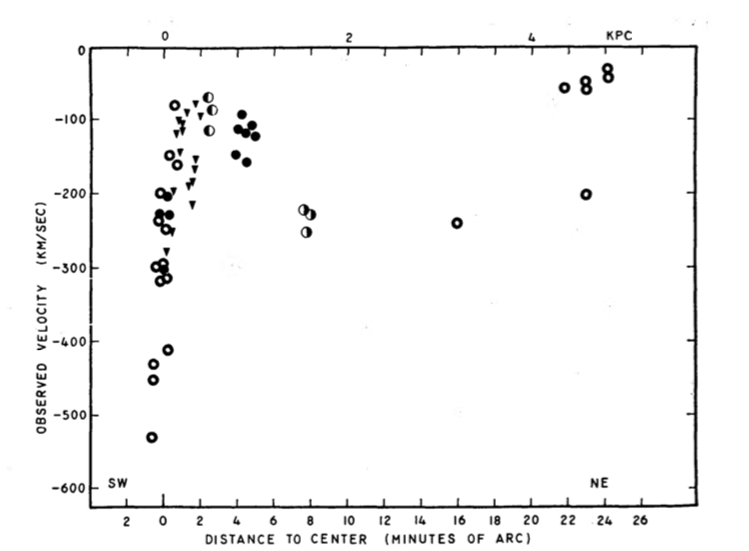
\includegraphics[width=\textwidth]{figs/RubinFordVel}
  \caption{The velocities of emission regions from M31 as a function of distance to the center of the galaxy measured in minutes of arc along the NE major axis as reported by Rubin and Ford in \cite{Rubin:1970zza}.}
\label{fig:rubin}
\end{figure}

Studies of the large scale structure of the universe have provided clues on the nature of dark matter. Just as on the small scale, ordinary visible matter consists of protons, electrons, neutrons, or groups of atoms held together by the electromagnetic force, analogously groups of massive stars and planets were bound together by the gravitational force in order to form stellar clusters. These groups were in turn merged with gas and the postulated DM to form galaxies, and the galaxies were bound together to form clusters, and subsequently superclusters. This standard theory of cosmic structure formation is often referred to as the ``bottom-up'' approach, and essentially posits that the current structure of the Universe is a result of the gravitational amplification of tiny matter fluctuations that were generated during the very early epochs of the Universe~\cite{Allen:2002eu}. The evidence from the 20th century for the existence of non-luminous matter has been further supplemented with data from weak~\cite{Refregier:2003ct} and strong~\cite{Tyson:1998vp} gravitational lensing by large scale structures. The distortion of the appearances of distant objects or the duplication of the apparent image is caused by the bending of the light these objects emit by the gravitational force of the large scale structures in between the observer and the object. The data from a survey of the Bullet cluster as observed by the Chandra~\cite{Markevitch:2005vi} experiment best illustrates how the distribution of the hot gas and stars originating from the collision of two galaxies and comprising the baryonic matter are bound together by a much greater contribution of non-luminous matter as seen in~\FigureRef{fig:bulletcluster}. The calculation of the approximate contribution of visible matter was performed using data from gravitational lensing.

\begin{figure}
  \centering
  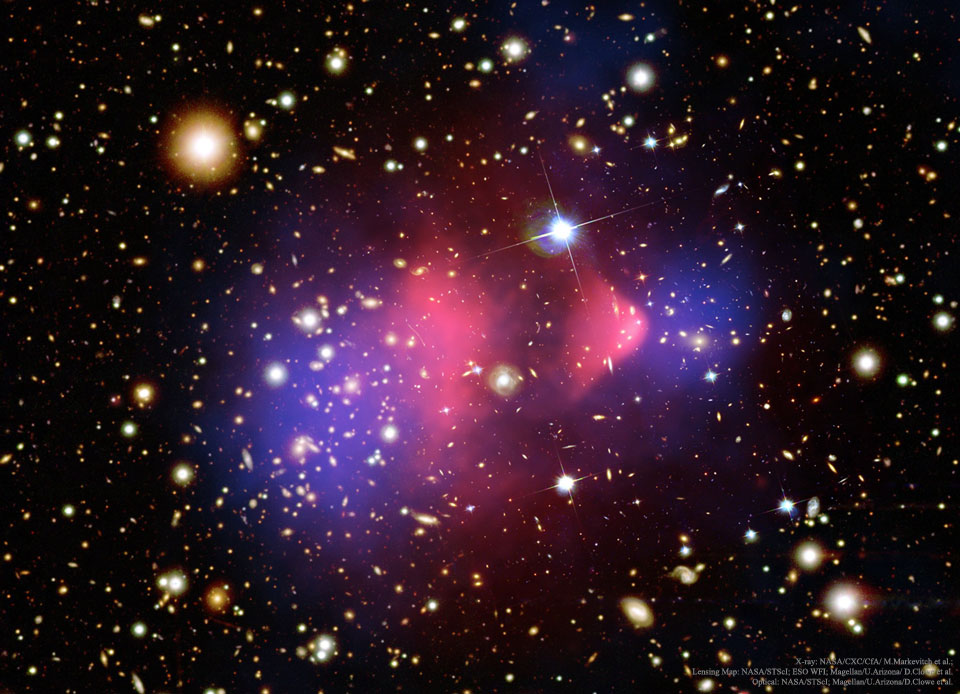
\includegraphics[width=0.8\textwidth]{figs/bulletcluster_comp_960.jpg}
  \caption{A composite image from the Hubble, Chandra, and Magellan telesopes of the 1E 0657-558 cluster of galaxies (Bullet cluster) depicting the X-rays emitted by the baryonic matter as a diffuse red gas, while the approximate location of the DM surrounding the visible matter is represented in a blue hue.}
\label{fig:bulletcluster}
\end{figure}

The aforementioned experiments and measurements buttress the necessity for the existence of DM, however the first attempts to precisely quantify the amount of DM in the Universe began with the discovery and subsequent analyses of the cosmic microwave background (CMB) by Peebles, Wilkinson, Dicke, and Roll~\cite{Dicke1965}. In brief, the CMB is the relic radiation energy content from beyond our galaxy, emitted shortly before the period of recombination~\cite{Seager:1999km} which occured approximately 380 000 years after the Big Bang. At this stage, photons began to decouple from the baryonic matter and over time have been redshifted to the microwave frequency range as a result of the expansion of the Universe over the past 13.81 billion years. Although the dominant contributions of the CMB are homogeneous and isotropic wherein the CMB temperature is almost uniformly $T\simeq2.72\:\mathrm{K}$, slight temperature fluctuations of $\mathcal{O}(10^{-5})$ have been observed which are indicative of the state of the early Universe and the relative abundance of visible and dark matter during this period. As gravity acted on the photon-baryon plasma, the fluid pressure increased giving way to its expansion. This cycle was repeated once the pressure decreased as a result of the expansion, and gravity once more won over causing a fluid compression, hence the photons emitted during different compression stages were of varying energies. More specifically, the period of photon decoupling leading to these relic temperature variations, known as the CMB anisotropy, can be interpreted as a power spectrum in terms of multipole orders, $\ell$. The effects produced by the acoustic oscillations of the photon-baryon plasma just prior to the emission of the CMB are captured in this spectrum. Since both types of matter contribute to the temperature oscillations via gravitational effects, the power spectrum shown in~\FigureRef{fig:CMB} contains information about the relative content of both visible and dark matter. The parametrization of the temperature anisotropies is in terms of spherical harmonics ($Y_{\ell m}$) contained in the two-dimensional function, $T(\theta,\phi)$ projected over the entire visible sky defined as,

\begin{equation}
  T(\theta,\phi) = \sum^{\infty}_{\ell=0}\sum^{\ell}_{m=-\ell}a_{\ell m}Y_{\ell m}(\theta,\phi),
\end{equation}

where $\theta$ and $\phi$ are angular coordinates, $\ell$ is the multipole order, and $a_{\ell m}$ are the multipole moments. Following the theory of temperature fluctuations, the distributions of the coefficients $a_{\ell m}$ are approximately Gaussian centered about zero with a variance defined as $C_{\ell} \equiv <|a_{\ell m}|^{2}>$, where there are only $2\ell+1$ values of $m$ for each $\ell$, hence

\begin{equation}
  C_{\ell} \equiv <|a_{\ell m}|^{2}> \equiv \frac{1}{2\ell+1}\sum^{+\ell}_{m=-\ell}|a_{\ell m}|^2.
\end{equation}

The power spectrum, $C_{\ell}$ is expressed as $\ell(\ell+1)C_{\ell}/2\pi$ in~\FigureRef{fig:CMB}, and the fit to the Planck data provides the abundances of baryonic and dark matter. The location of the first peak is related to the flat geometry of the Universe and requires that the total energy-matter density ratio, $\Omega_\mathrm{total}=1$. The resolution of this peak is connected to the expansion of the Universe which is driven by the repulsive force of dark energy~\cite{Spergel:2006hy}. The angular resolution of the second peak, at $\ell_{2}\simeq500$, provides the amount of ordinary matter that exists in the Universe, and correspondingly, the difference between the third peak, at $\ell_{3}\simeq700$, and the second peak provides the density of the dark matter in the early Universe. The extracted total densities of baryonic and dark matter are respectively,

\begin{equation}
  \Omega_{\mathrm{b}}h^2 = 0.02222 \pm 0.00023,\:\:\Omega_{\chi}h^2 = 0.1186 \pm 0.0020,
\end{equation}

where $h = H_{0}/100$ is the reduced Hubble's constant. The relic abundances tranlsate to $24\%$ and $4.8\%$ of the total matter in the Universe as being dark and baryonic, respectively, while the rest consists of dark energy~\cite{Agashe:2014kda}.

\begin{figure}
  \centering
  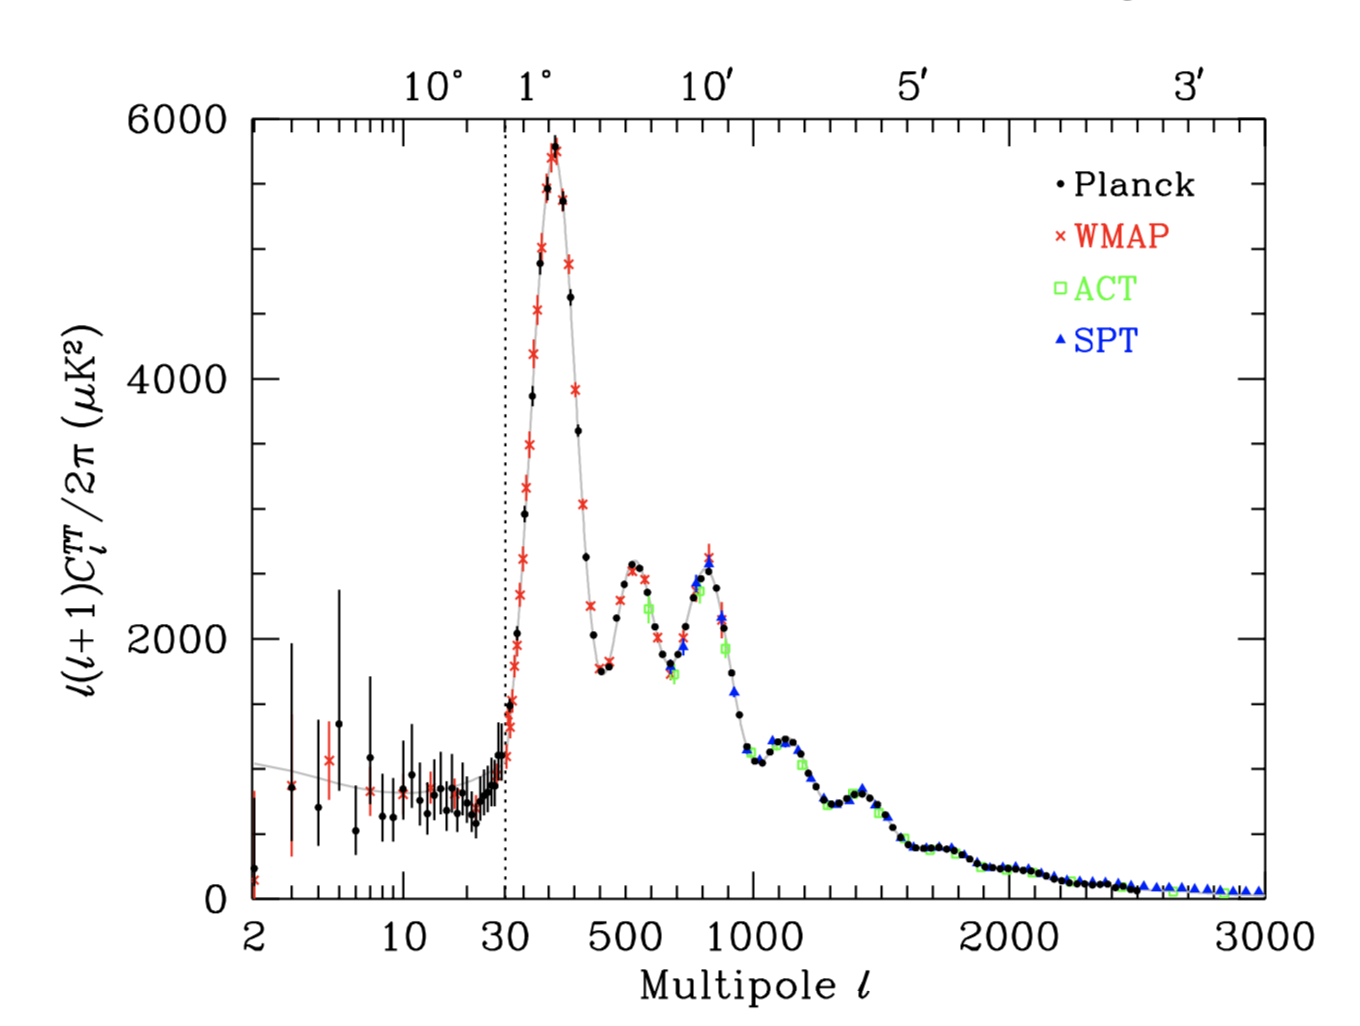
\includegraphics[width=0.8\textwidth]{figs/CMB_multipole}
  \caption{The CMB radiation temperature anisotropy power spectrum as a function of the multipole order,$\ell$, as measured by various experiments~\cite{Agashe:2014kda}. The angular scales that correspond to the multipole orders are listed across the top of the graph. The data points correspond to the experimental measurements and the error bars account for measurement uncertainties. The black curve represents the best global fit of the standard model of cosmology to the Planck data.}
  \label{fig:CMB}
\end{figure}

%In addtion, the numerical simulations  The observation that star ages within galaxies are on the order of 10 to 14 billion years old, and cluster formation is still under way serves to support the cold dark matter (CDM) hypothesis. In this case, DM comprises of rather massive, slow moving, and non-relativistic particles, which would stimulate the clumping of matter into small regions initially, eventually giving rise to larger scale structures. This bottom-up theory of structure formation is further supported by myriad computer simulations consisting of billions of dark matter particles confirming the CDM model yields large structures such as those observed by the Sloan Digital Sky Survey. 

\section{The Standard Model}
\label{sec:SM}

In the pursuit of a suitable candidate for what comprises close to $24\%$ of the total matter in the Universe, a segue to the fundamental underpinnings of the SM of particle physics is required. In this section, an overview of the SM is presented along with its most successful predictions of experimentally observed particle physics phenomena and its greatest deficiencies in the quest to explain the nature of DM. 

As a framework that describes the fundamental constituents of observed matter and their corresponding interactions, in this respect the SM is deemed exceedingly successful. Not only are such observations predicted accurately by the SM, but its organization of the fundamental building blocks of our Universe within a framework can be thought of as analagous to the organization of elements within Mendeleev's periodic table~\cite{PhysRevD.86.010001}. In the theory of the SM, three of the four fundamental forces are responsible for particle matter interactions: the electromagnetic, weak, and strong forces. A few of the matter particles which these forces act upon include protons, neutrons, electrons, and quarks, whose properties are described in detail later in this section. An example of particle interactions described by the SM is the binding of neutrons and protons via the strong force in the atomic nucleus. By contrast, the weak force is responsible for the process of a neutron decaying to a proton, during which one type of quark is transmuted to another (nuclear $\beta$ decay). The electromagnetic (EM) force is responsible for such phenomena as Bremsstrahlung, the process of EM radiation as a result of the deceleration of a charged particle deflected off another charged particle. 

The foundations of the SM began with the unification of the weak and electromagentic forces in the Glashow-Weinberg-Salam (GWS) theory of electroweak (EW) interactions~\cite{Glashow:1959wxa, Salam:1968rm, PhysRevLett.19.1264} leading to the theory of quantum electrodynamics (QED), and making the first firm prediction of mass possible~\cite{Griffiths:111880}. The strong force is described by what constitutes as the remainder of the SM, the theory of quantum chromodynamics (QCD)~\cite{PhysRevLett.30.1346,PhysRevLett.30.1343}. The remaining of the four fundamental forces, gravity, does not have a place within the SM as of yet, as it is a quantum theory used to describe the ``micro'' world and is difficult to fit into the same framework as Einstein's general theory of relativity describing the ``macro'' world, where gravity plays a significant role. Acting with vastly larger strengths over significantly shorter ranges, the EW and strong forces render the effects of gravity negligible in the context of particle physics phenomena. 

The elementary matter components of the SM are particles obeying Fermi-Dirac statistics called \textit{fermions} and have half-integer spins, while the force carriers or so-called ``messenger'' particles obey Bose-Einstein statistics, known as \textit{bosons} have integer spin. Individual fermion particle states can interact via the strong force to form \textit{baryons} such as the proton and the neutron, which consist of three \textit{quarks} (the elementary fermion particles comprising the substructure of the nucleon). Similarly, a \textit{meson} is a bosonic two-fermion bound state consisting of a quark and anti-quark pair. Any particles, whether composite like baryons or mesons, or elementary like the quark, which interact via the strong force are classed as \textit{hadrons}. Of course, there are also fermions like the electron and the neutrino which do not interact via the strong force, but rather via the electromagentic (EM), which are called \textit{leptons}. The elementary quarks, leptons, and bosons carry quantum numbers that dictate their interactions such as charge (Q), lepton number (L), baryon number (B), and spin. It should be noted that color charge (C), weak isospin (T$_{3}$), and hypercharge (Y) are also additional elementary particle quantum numbers that characterize the symmetry groups comprising the SM to be introduced later. The leptons and quarks listed in the first six rows of Table~\ref{tab:SM} are divided into three generations where a mass hierarchy is established with increase in generation. Despite the increase in mass with generation, the lifetime in general decreases, although $c$ and $b$ quarks are an exception to this trend, providing an experimental handle for their discrimination in high energy experiments. In addition, quarks and leptons of higher generations can decay to quarks and leptons of the corresponding first generation. The bottom five rows in Table~\ref{tab:SM} list the weak force carrying bosons, W and Z, the strong force carrying boson, g, the EM force carrying boson, $\gamma$, and the Higgs boson, H, which gives the other particles mass.  

\begin{table}[!htbp]
  \scalebox{0.85}{
    \begin{tabular}{l l l c c c l}
      \hline
      & Particle & Particle &      & Electric    & Mass  & Force\\
      Generation & Symbol   & Name     & Spin & Charge      & [GeV] & Interaction/Carrier \\
      \hline
      1st        & $e^-$    & Electron          & 1/2  & -1  & $5.11\times10^{-4}$ & EM, Weak \\
      & $\nu_{e}$& Electron Neutrino & 1/2  & 0   &  -                  & Weak \\
      \hline   
      2nd        & $\mu^-$     & Muon          & 1/2  & -1 & 0.106        & EM, Weak \\
      & $\nu_{\mu}$ & Muon Neutrino & 1/2  & 0  &  -           & Weak \\
      \hline
      3rd        & $\tau^-$     & Tau          & 1/2  & -1 & 1.78        & EM, Weak \\
               & $\nu_{\mu}$  & Tau Neutrino & 1/2  & 0  &  -           & Weak \\
      \hline \hline
      1st        & $u$          & Up Quark   & 1/2 & 2/3      & $\approx2.3\times10^{-3}$ & EM, Weak, Strong \\
      & $d$          & Down Quark & 1/2 & -1/3     & $\approx4.8\times10^{-3}$ & EM, Weak, Strong \\
      \hline
      2nd        & $s$          & Strange Quark & 1/2 & -1/3  & $\approx9.5\times10^{-2}$ & EM, Weak, Strong \\
      & $c$          & Charm Quark   & 1/2 & 2/3 & 1.28                      & EM, Weak, Strong \\
      \hline
      3rd        & $b$          & Bottom Quark  & 1/2 & -1/3 & 4.2                      & EM, Weak, Strong \\
               & $t$          & Top Quark     & 1/2 & 2/3  & 172.5                    & EM, Weak, Strong \\
      \hline \hline
      -          & W$^\pm$      & W Boson       & 1   & $\pm1$ & 80.4                   & Weak \\ 
      -          & Z            & Z Boson       & 1   &    0   & 91.2                   & Weak \\
      -          & $\gamma$     & Photon        & 1   &    0   & 0                      & EM   \\
      -          & g            & Gluon         & 1   &    0   & 0                      & Strong \\
      \hline\hline
      -          & H            & Higgs Boson   & 0   &    0   & 125                    & - \\
      \hline
    \end{tabular}
  }
  \caption{The particles of the SM including the leptons ($e^-$, $\mu^-$, $\tau^-$, $\nu_{e}$, $\nu_{\mu}$, $\nu_{\tau}$), the quarks ($u$, $d$, $c$, $s$, $t$, $b$), the gauge bosons (W$^\pm$, Z, g, $\gamma$), and the scalar Higgs boson (H). The spin, charge, and mass are specified where the neutrinos are taken to be massless, and indirect measurements posit the mass eigenstates are less than 0.23 eV~\cite{PhysRevD.86.010001}. The forces via which the particles interact are listed for each lepton and quark and the force mediated is listed for the gauge bosons.}
  \label{tab:SM}
\end{table}

The SM is defined in terms of a quantum field theory (QFT) Lagrangian density that adheres to certain symmetries. Just as the classical field theory of electricity and magnetism, as fully described by Maxwell's equations, remains unchanged under position, rotation, reflection, and Lorentz transformations, so the SM remains invariant under certain transformations, better known as symmetries. In the case of Maxwell's equations, when invariance under the standard translational, rotational, and reflectional symmetries are combined with invariance under Lorentz symmetry, the combined group of symmetries is termed the Poincar$\acute{\mathrm{e}}$ Lie group. The Poincar$\acute{\mathrm{e}}$ symmetry is a global (spacetime) symmetry, whereas the Lie groups of the symmetries associated with the SM are local transformations associated with fields rather than particles defined by space and time coordinates. The local or internal symmetries which are the starting point for the various parts of the SM Lagrangian, are also known as gauge symmetries. The interactions within the SM are described by specific interaction terms which modify the Lagrangian leaving it invariant under the gauge transformations. Hence, the SM is defined as a gauge QFT based on the $SU(3)_{C}\otimes SU(2)_{L}\otimes U(1)_{Y}$ symmetry groups, where the elementary particle interactions dictated by the strong force are described by the $SU(3)_{C}$ Lie group, and interactions dictated by the electroweak forces are described by $SU(2)_{L}\otimes U(1)_{Y}$.

\subsection{Electroweak theory and the Higgs mechanism}
\label{subsec:EWKHiggs}

The point of departure for the description of interactions in the SM is the Dirac Lagrangian density,

\begin{equation}
  \mathcal{L}_{D} = \bar{\psi}(i\gamma^\mu\partial_\mu - m)\psi,
  \label{eq:dirac}
\end{equation}

where $\gamma^\mu$ are the Dirac $\gamma$-matrices, $\bar{\psi} = \gamma^{0}\psi$ is the conjugate fermion field, and $m$ is the fermion mass. Defining the interactions between a two spin-$\frac{1}{2}$ fields, which can be re-written as the doublet, 

\begin{equation}
  \Psi := 
  \begin{pmatrix}
    \psi_{1} \\
    \psi_{2}
    \end{pmatrix},
  \label{eq:doublet}
\end{equation}

requires a locally $SU(2)$ invariant Lagrangian achieved through the addition of the extra term $i\bar{\Psi}\gamma_\mu \frac{\sigma_i}{2} W^\mu_i \Psi$ which describes the interactions between two spin-$\frac{1}{2}$ and three massive spin-1 fields $W^\mu_i$. This process exploits a local internal symmetry of $W^\mu_i$ where $W^\mu_i \rightarrow W^{'\mu}_i = W^\mu_i + \partial^\mu a_i(x)$. Neglecting the mass terms, the Lagrangian then reads,

\begin{equation}
  \mathcal{L}_{D1+D2+int} = i\bar{\Psi}\gamma_\mu\partial^\mu\Psi + \bar{\Psi}\gamma_\mu \frac{\sigma_i}{2} W^\mu_i \Psi,
  \label{eq:partialQED}
\end{equation}

but \EquationRef{eq:partialQED} is missing the term for the three free spin-1 fields which includes the internal symmetry as described above. When this term is added, \EquationRef{eq:partialQED} turns into,

\begin{equation}
  \mathcal{L}_{SU(2)} = i\bar{\Psi}\gamma_\mu\partial^\mu\Psi + \bar{\Psi}\gamma_\mu \frac{\sigma_i}{2} W^\mu_i \Psi - \frac{1}{4}(W_{\mu\nu})_{j}(W^{\mu\nu})_{j},
  \label{eq:SU2}
\end{equation}

with $(W_{\mu\nu})_i = \partial_\mu(W_\nu)_i  - \partial_\nu(W_\mu)_i$, and leading to an $SU(2)$ invariant Lagrangian. \EquationRef{eq:SU2} is nonetheless lacking mass terms because the introduction of terms such as $m_{1}\bar{\Psi}{\Psi}$ or $m_{2}(W^\mu)_i(W_\mu)_i$ would destroy the $SU(2)$ symmetry. Acquiring the mass terms will be done through the breaking of this symmetry by the addition of a spin-0 field. Before this however, it is possible to unify the locally $SU(2)$ invariant Lagrangian in \EquationRef{eq:SU2} with a locally $U(1)$ invariant Lagrangian in order to additionally describe fermion EM interactions. Hence, the spin-1 field $B^\mu$, also known as the $U(1)$ gauge field, is introduced where its locally $U(1)$ invariant Lagrangian goes as,

\begin{equation}
  \mathcal{L}_{U(1)} = -m\bar{\psi}\psi + \bar{\psi}\gamma_\mu(i\partial^\mu + gB^\mu)\psi - \frac{1}{4}B_{\mu\nu}B^{\mu\nu}
  \label{eq:U1}
\end{equation} 

where $B^{\mu\nu} := \partial^\mu B^\nu - \partial^\nu B^\mu$. Combining \EquationRef{eq:SU2} and \EquationRef{eq:U1} then yields the $SU(2)$ and $U(1)$ locally invariant Lagrangian,

\begin{equation}
  \mathcal{L}_{SU(2)\otimes U(1)} = \bar{\Psi}\gamma_\mu(i\partial^\mu + gB^\mu + g'\sigma_i W^\mu_i)\Psi - \frac{1}{4}(W_{\mu\nu})_{j}(W^{\mu\nu})_{j}-\frac{1}{4}B_{\mu\nu}B^{\mu\nu},
  \label{eq:SU2cU1}
\end{equation}

where the coupling constant for the three $W^\mu_i$ fields is ignored and simply denoted by $g'$. As mentioned earlier, the mass terms cannot be added ``by hand'' to the Lagrangian since they effectively spoil the symmetry, but by writing a locally $SU(2)$ invariant Lagrangian for doublets of spin-0 fields, just as done in \EquationRef{eq:partialQED} earlier for spin-$\frac{1}{2}$ fields, it will be shown how the mass terms for the $W^\mu_i$ and $B^\mu_i$ fields are attained. Thus for the spin-0 doublet $\Phi := \begin{pmatrix} \phi_1 \\ \phi_2 \end{pmatrix}$, \EquationRef{eq:SU2cU1} turns into,

\begin{equation}
  \begin{aligned}
  \mathcal{L}_{SU(2)\otimes U(1)} = ((\partial_\mu - ig'\sigma_i(W_\mu)_i - i\frac{1}{2}gB_\mu)\Phi^{\dagger})((\partial^\mu - ig'\sigma_i(W^\mu)_i + i\frac{1}{2}gB^\mu)\Phi) \\
  + \rho^2\Phi^\dagger\Phi - \lambda(\Phi^\dagger\Phi)^2,
  \end{aligned}
\label{eq:b4symbreak}
\end{equation}

where the last two terms on the right-hand side are defined collectively as $-V(\Phi)$, or are better known as the Higgs potential. $V(\Phi)$ can in fact be written as a function of one of the spin-0 doublet fields, $V(\phi)$, so that the minimum of $V(\phi) = -\rho^2|\phi|^2 + \lambda|\phi|^4$ can be computed in the traditional way by $\frac{\partial V(\phi)}{\partial\phi} = 0$. This leads to a minimum $\phi_{\mathrm{min}} = \sqrt{\frac{\rho^2}{2\lambda}}e^{i\phi}$ meaning that for every $\phi$ value there exists a minimum and thus there are an infinite number of minima, all of which lie on a circle with radius $\sqrt{\frac{\rho^2}{2\lambda}}$. Best visualized by the 3-dimensional $V(\phi)$ function in the complex plane in ~\FigureRef{fig:mexhat}, a minimum is chosen out of the infinite possibilities (i.e. symmetry breaking), in the same sense that a marble would roll down from the top of the ``sombrero'' potential and spontaneously or randomly choose a vacuum value to settle in, out of infinite possibilities. 

\begin{figure}
  \centering
  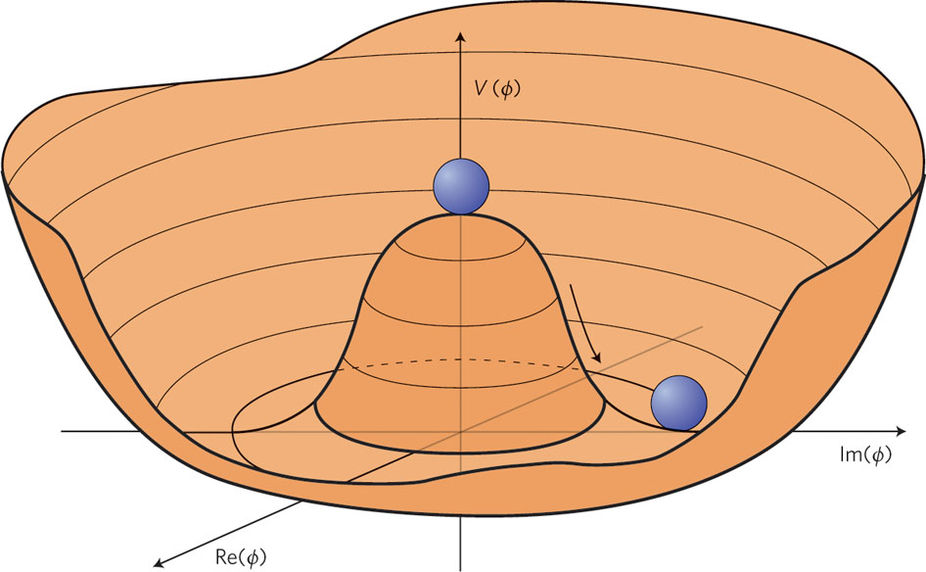
\includegraphics[width=0.7\textwidth]{figs/mexhat}
  \caption{The vacuum value, or the lowest-energy state, of the Higgs potential as shown in the 3-dimensional plot is described by a randomly chosen point at the bottom of the ``sombrero''~\cite{Alvarez-Gaume:2010aa}.}
  \label{fig:mexhat}
\end{figure}

The spin-0 doublet can then be re-written as,

\begin{equation}
  \Phi_{\mathrm{min}} = \begin{pmatrix} 0 \\ \sqrt{\frac{\rho^2}{2\lambda}} \end{pmatrix} \equiv \begin{pmatrix} 0 \\ \frac{v}{\sqrt{2}} \end{pmatrix},
  \label{eq:higgsdoublet}
\end{equation}

where the redefinition of the minimum in terms of $v$ is chosen for brevity. Substituting the field $\Phi$ with the minimum shifted field in what is known as the unitary gauge, $\Phi_{\mathrm{min}}$, and subsequently performing the matrix algebra of the first term in \EquationRef{eq:b4symbreak}, the following expression is attained,

\begin{equation}
  \frac{v^2}{8}(g')^2((W^\mu_1)^2 + (W^\mu_2)^2) + (g'W^\mu_3 - gB^\mu)^2),
  \label{eq:massbreak}
\end{equation} 

where two new spin-1 fields can be defined from the old ones,

\begin{equation}
  W^\mu_{+} \equiv \frac{1}{\sqrt{2}}(W^\mu_1 -iW^\mu_2) \\
  W^\mu_{-} \equiv \frac{1}{\sqrt{2}}(W^\mu_1 +iW^\mu_2),
\end{equation}

where $W^\mu_{+}$ and $W^\mu_{-}$ are complex conjugates of one another, and the first term in \EquationRef{eq:massbreak} becomes $\frac{1}{8}v^2g'^{2}(W^+)_\mu(W^-)^\mu$. At last, the W boson mass term ($\frac{1}{2}M_{W}^2 = \frac{1}{8}v^2g'^{2}$) is given! Similarly, the second term in \EquationRef{eq:massbreak} can be expanded with matrix diagonalization, and the remaining spin-1 fields, $W^\mu_3$ and $B^\mu$, can be interpreted in terms of the new spin-1 fields, 

\begin{equation}
  Z_\mu = W^\mu_3\cos{\theta_W} - B^\mu\sin{\theta_W}, \\
  A^\mu = W^\mu_3\sin{\theta_W} + B^\mu\cos{\theta_W},
\end{equation} 

where $\theta_W$ is the weak mixing angle (or Weinberg angle), and is given by $\tan^{-1}(\frac{g'}{g})$ and the terms in \EquationRef{eq:massbreak} become,

\begin{equation}
  \frac{1}{8}v^2g'^{2}(W^+)_\mu(W^-)^\mu + \frac{1}{8}v^2\frac{g'^{2}}{\cos{\theta_W}^2}Z_\mu^2 + \frac{1}{8}v^2\cdot0\cdot A_\mu^2.
  \label{eq:EWmass}
\end{equation}

The fields can then be identified with the bosons in Table~\ref{tab:SM} where $A_\mu$ is the photon. The masses of the fields can be read off as,

\begin{equation}
  \begin{split}
    & M_W = \frac{g'v}{2} \\ 
    & M_Z = \frac{g'v}{2\cos{\theta_W}} = \frac{M_W}{\cos{\theta_W}} \\ 
    & M_A = 0 
  \end{split}
\end{equation}

Hence, the Higgs mechanism is the means by which the gauge theory of massless bosons, after symmetry breaking, becomes a theory of masssive bosons. In addition, the Higgs field vacuum expectation value, $v$ is 246 GeV. From the steps above which lead to the field responsible for the Z boson $Z_\mu$ and the field responsible for the photon $A_\mu$, it can be seen that both have a common point of departure, since they are orthogonal linear combinations of the fields $B_\mu$ and $W_\mu^3$. 

\subsection{Yukawa interactions}
\label{subsec:yukawa}

In addition to allowing bosons to have mass, the Higgs mechanism gives fermions their masses without destroying gauge invariance after symmetry breaking. This is a particularly attractive feature of the SM, since the same Higgs doublet that generates the $W^\pm$ and Z masses suffices to allow for lepton and quark masses. In order to ensure that gauge invariance is retained, the new interaction terms in the Lagrangian between the spin-$\frac{1}{2}$ fields and the spin-0 Higgs field with the doublet as $\Phi := \frac{1}{\sqrt{2}}\begin{pmatrix} 0 \\ v + h \end{pmatrix}$, where h describes a physical Higgs boson, is

\begin{equation}
  \mathcal{L}_{Hf\bar{f}} = -(h_d)_{ij}\bar{q}_{L_i}\Phi d_{R_j} - (h_u)_{ij}\bar{q}_{L_i}(-i\sigma_2\Phi^*)u_{R_j} - (h_\ell)_{ij}\bar{\ell}_{L_i}\Phi \ell_{R_j}.
  \label{eq:fermioncoupling}
\end{equation}

From this, it can be seen that the Higgs couples to quark doublets, which are left chiral states (L) under $SU(2)$ transformations, and to either up or down-type right chiral (R) quark singlets (i.e. $u_{R}$ and $d_{R}$). The Higgs doublet also has couplings to left-handed lepton doublets and charged right-handed lepton singlets. Once the $SU(2)\otimes U(1)$ symmetry is spontaneously broken then \EquationRef{eq:fermioncoupling} becomes,

\begin{equation}
  \mathcal{L}_{m_f} = (m_d)_{ij}\bar{d}_{L_i}d_{R_j} + (m_u)_{ij}\bar{u}_{L_i}u_{R_j} + (m_e)_{ij}\bar{e}_{L_i}e_{R_j},
  \label{eq:fermionmass}
\end{equation}

where $m_{f} = \frac{y_{f}v}{\sqrt{2}}$, with $y_f$ being the Yukawa coupling for a fermion $f$. $u_L$, $d_L$, and $e_L$ are the up-type quark, down-type quark and lepton doublet components defined as,

\begin{equation}
\begin{split}
&  \begin{pmatrix} 
    u \\
    d'
  \end{pmatrix}_L
  \begin{pmatrix} 
    c \\
    s'
  \end{pmatrix}_L
  \begin{pmatrix} 
    t \\
    b'
  \end{pmatrix}_L
  \\
&  \begin{pmatrix} 
    \nu_e \\
    e
  \end{pmatrix}_L
  \begin{pmatrix} 
    \nu_\mu \\
    \mu
  \end{pmatrix}_L
  \begin{pmatrix} 
    \nu_\tau \\
    \tau
  \end{pmatrix}_L
\end{split}
\end{equation}

Thus, the relation between the fermion mass and the Yukawa coupling demonstrates that heavier fermions correspond to fields that are more strongly coupled to the Higgs boson. In order to go from the quark weak eigenstates ($d'$, $s'$, $b'$) to the corresponding mass eigenstates, the Cabbibo-Kobayashi-Maskawa (CKM) matrix below is used,

\begin{equation}
  \begin{pmatrix}
    d' \\
    s' \\
    b'
  \end{pmatrix} 
  =
  \begin{pmatrix}
    V_{ud} & V_{us} & V_{ub} \\
    V_{cd} & V_{cs} & V_{cb} \\
    V_{td} & V_{ts} & V_{tb}
  \end{pmatrix}
  \begin{pmatrix}
    d \\
    s \\
    b
  \end{pmatrix}
  \label{eq:CKM}
\end{equation} 

where the CKM matrix values are, 

\begin{equation}
  \begin{pmatrix}
    V_{ud} & V_{us} & V_{ub} \\
    V_{cd} & V_{cs} & V_{cb} \\
    V_{td} & V_{ts} & V_{tb}
  \end{pmatrix}
 = 
\begin{pmatrix}
  0.974 & 0.225 & 0.004 \\
  0.225 & 0.973 & 0.041 \\ 
  0.009 & 0.040 & 0.999
\end{pmatrix}
\end{equation}

It can be noted that the CKM matrix is nearly the identity, thus transitions between fermion generations are heavily suppressed, but by contrast a top quark decays to a W boson and b quark at a rate of $99.9\%$. Quark couplings to the W boson are in part characterized by the CKM matrix in what follows as the Lagrangian for charged currents,

\begin{equation}
  \mathcal{L}_{\mathrm{CC}} = \frac{g}{\sqrt{2}}W_\mu^+(\nu_L \gamma^\mu e_L + V_{\mathrm{CKM}}\bar{u}_L\gamma^\mu d_L) + \frac{g}{\sqrt{2}}W_\mu^-(\bar{e}_L\gamma^\mu\nu_L + V_{\mathrm{CKM}}\bar{d}_L\gamma^\mu u_L),
\end{equation}

where $u$ denotes up-type quarks, $d$ denotes down-type quarks, $\nu$ denotes neutrinos, and $e$ denotes charged leptons. From the subscript, it can be noted that only left-handed fermions (and right-handed antifermions) couple to the W$^\pm$, hence there is a 100$\%$ breaking of parity ($\mathcal{P}$) and charge conjugation ($\mathcal{C}$), however gauge invariance is still preserved under the combined $\mathcal{CP}$ symmetry. Similarly, quarks and leptons couple to the neutral carriers of electroweak interactions, the Z boson and the photon, via the neutral current Lagrangian given by,

\begin{equation}
  \mathcal{L}_{\mathrm{NC}} = \sum_{j}\bar{\psi}_j \gamma^\mu\ \Big\{ A_\mu [g \frac{\sigma_3}{2}\sin\theta_W + g'y_j \cos\theta_W] + Z_\mu[g\frac{\sigma_3}{2}\cos\theta_W - g'y_j\sin\theta_W] \Big\}\psi_j,
\end{equation}

where for simplicity we take,

\begin{equation} 
  \psi_1 = \begin{pmatrix} u \\ d \end{pmatrix}_L, \:\:\: \psi_2 = u_R, \:\:\: \psi_3 = d_R,\:\mathrm{or} \\
  \psi_1 = \begin{pmatrix} \nu_e \\ e^- \end{pmatrix}_L, \:\:\: \psi_2 = {\nu_e}_R, \:\:\: \psi_3 = {e^-}_R.
\end{equation}

The EM coupling is defined as $e = g\sin\theta_W = g'\cos\theta_W$ and a relation between the fermion hypercharge ($Y$), electric charge ($Q$) and weak isospin ($T_3$) quantum numbers can be established with $T_3 \equiv \sigma_3/2$ and $Y = Q - T_3$. Hence, for quarks and leptons,

\begin{equation}
  \mathrm{Quarks:}\: y_1 = Q_u - \frac{1}{2} = Q_d + \frac{1}{2} = \frac{1}{6},\:\:\:\:\: y_2 = Q_u = \frac{2}{3}, \:\:\:\:\: y_3 = Q_d = -\frac{1}{3}, \\
  \mathrm{Leptons:}\: y_1 = Q_\nu - \frac{1}{2} = Q_e + \frac{1}{2} = -\frac{1}{2},\:\:\:\:\: y_2 = Q_\nu = 0, \:\:\:\:\: y_3 = Q_e = -1.
\end{equation}

Thus, it is shown that fermions with the same electric charge have the same universal couplings, and neutrinos do not have EM interactions ($Q_\nu=0$) although their coupling to the W and Z boson is non-zero. Examining the properties of the neutrino more closely, one might be tempted to propose it as a viable DM particle candidate since it satisfies \textit{some} of the key requirements for a suitable candidate, those being:

\begin{itemize}
  \item Stability on the order of the cosmic timescale, as required to remain in existence currently
  \item No strong or EM interactions
  \item Non-baryonic, since the potential baryon fraction of DM is known to be small
  \item Combined with any other DM particles/constituents, the total DM must have the correct relic density
\end{itemize}

It will however, become clear in the following section, why the neutrino, as predicted by the SM, is an insufficient contender for $24\%$ of the matter fraction in the Universe. Analogously, the SM, as briefly described in this section, successfully predicts observed particle physics phenomena to a high degree of accuracy, with the most recent experimental confirmation being the discovery of a $125\:\GeV$ particle compatible with the predicted Higgs boson, by the ATLAS and CMS experiments at the LHC in 2012~\cite{Aad:2012tfa,Chatrchyan:2012xdj}. Nonetheless, there exist a number of theoretical and phenomenological problems, which cannot be accommodated by the SM. Among those are the hierarchy problem, wherein the Planck scale ($M_{Pl} \sim 10^{18}\:\GeV$), the point at which gravity is as strong as the gauge interactions, is nearly $\mathcal{O}(10^{15})$ larger than the electroweak scale, both of which are widely considered fundamental energy scales in nature. In addition, the matter-antimatter asymmetry that exists in the Universe today does not jive with the SM prediction that approximately equal amounts of matter and antimatter should have been created during the earliest phases of the Universe, had a proportionate amount of matter compared to antimatter existed during the initial conditions. Other open issues such as the addition of small, but nonetheless experimentally observed neutrino mass~\cite{Feldman:2013vca} to the SM is not possible unless other key free parameters are modified which leads to further theoretical complications of the SM framework. Alongside these open questions is the lack of a fundamental particle candidate supplied by the SM to explain the vast amount of DM in as observed in the Universe. Possible extensions to the SM can help to alleviate the tension presented between the above physical phenomena and the to-date widely accepted model, where the hints of BSM physics would manifest as experimental observations of deviations from SM processes.

\section{Dark matter candidates}
\label{sec:DMcandidates}

Returning to the example of a neutrino as a possible particle DM candidate can help to elucidate the properties which have lead to the most dominant model, currently. During the early stages of the Universe, when the rate of cosmic expansion overtook the rate at which weak interactions in equilibrium proceeded, such as neutron-proton conversion given by $n \leftrightarrow p + e^- + \bar{\nu}_e$, the process of SM neutrino decoupling from the background radiation occured. At this so-called ``freeze out'' stage, the neutrino is relativistic and remains as such during the later stages of galaxy and larger structure formation, owing also to its near massless nature. Relativistic particles moving throughout the Universe, however, are generators of high pressure, which cause a smoothening and subsequent destruction of any small matter density fluctuations and would ultimately not lead to the large scale structure formation as observed today. Evidence from N-body simulations made as early as 1983 by White, Frenk, and Davis~\cite{White:1984yj} present a vastly inconsistent picture of galaxy clustering than what is observed, and consequently definitively rule out a neutrino-dominated Universe.

The SM neutrino is part of a larger classification of particle DM, known as hot dark matter (HDM). HDM candidates are very light particles with $m_{\mathrm{HDM}} < 1\:\mathrm{eV}$, and are typically disfavored as leading candidates since they hinder large scale structure formation as a result of their relativistic energies. Although HDM certainly exists in our Universe today, such as SM neutrinos, current observational data place an upper limit of $0.25\%$ of the fraction of mass in the Universe as contributed by HDM. On the other hand, at the other end of the energy spectrum are DM candidates which are non-relativistic at the time of decoupling from the thermal bath, and are classed as cold dark matter (CDM). With a mass ranging between $\mathcal{O}(\GeV) < m_\mathrm{CDM} < \mathcal{O}(\TeV)$, the lower velocities of CDM in contrast to those of HDM would result in a short range dispersion with respect to the size of the Universe, and generate very little pressure, allowing for the clustering of stars and galaxies to form the filaments and structures observed today. Numerous N-body simulations commencing from random density fields of non-interacting CDM demonstrate these observations~\cite{10.1093}. Situated between HDM and CDM, warm dark matter (WDM), is postulated to have $m_{\mathrm{WDM}} \simeq \mathcal{O}(\mathrm{keV})$. Although relativistic at the time of decoupling, WDM then cools during the radiation-to-matter transition phase and becomes non-relativistic causing some smoothening of dense knots of matter, but still allowing for structure formation. Sterile neutrinos, gravitinos, and photinos fall under this category, but WDM is disfavored in large part because N-body simulations are less consistent with observations than those for CDM candidates.

The leading DM candidate, which is classified as a type of CDM, is the weakly interacting massive particle (WIMP) and to-date it is the most theoretically desirable candidate for a number of reasons. One of the strongest arguments for a WIMP as a DM candidate, should it exist and be stable, is that the relic density it would produce is consistent with that required by DM. The mechanism via which this occurs is referred to as the ``WIMP miracle'', alluding to the notion that WIMPs, although originally proposed as a solution to the gauge hierarchy problem, are extremely suitable DM candidates as well. As mentioned earlier, the thermal freeze-out period of the Universe occured when interactions with the thermal bath which reach an equilibrium can no longer keep up with the rate of expansion of the Universe, hence after freeze-out, interactions which affect the total number of WIMPs are negligible. The exchange of energy between SM particles and WIMPs may still proceed efficiently, however. Quantitatively, the number density of the DM particle, $n$, can be described by the Boltzmann equation,

\begin{equation}
  \frac{dn}{dt} = -3Hn - \langle\sigma_A v \rangle(n^2 - n_{\mathrm{eq}}^2),
  \label{eq:boltz}
\end{equation}

where H is the Hubble constant, $\langle\sigma_A v\rangle$ is the thermally averaged annihilation cross section and $n_{\mathrm{eq}}$ is the DM number density in thermal equilibrium. In order to obtain the thermal relic density, \EquationRef{eq:boltz} is solved numerically, where the freeze-out time is defined as $n\langle\sigma_{A} v\rangle = H$ and leads to~\cite{PhysRevD.33.1585},
\begin{equation}
  \Omega_{\chi} \simeq \frac{\mDM T_0^3}{\rho_c M_{Pl} T_f} (\langle \sigma_A v \rangle)^{-1},
\label{eq:Omega}
\end{equation}
where $\rho_c$ denotes the critical density, $\mDM$ denotes the DM mass, and $T_0$ and $T_f$ denote the present and freeze-out time temperatures. It can be noted that $\Omega_{\chi}$ has an inversely proportional relationship to the velocity-averaged annihilation cross section and does not strongly depend on the mass of the DM. Thus, for WIMPs postulated to be in the $\mathcal{O}(\GeV) < \mDM < \mathcal{O}(\TeV)$ mass range, assuming that the annihilation cross section into SM particles is on the order of the electroweak scale, the observed $\Omega_{\chi}$ is correctly predicted by the WIMP miracle, as visualized in~\FigureRef{fig:WIMPrelic}.

\begin{figure}
  \centering
  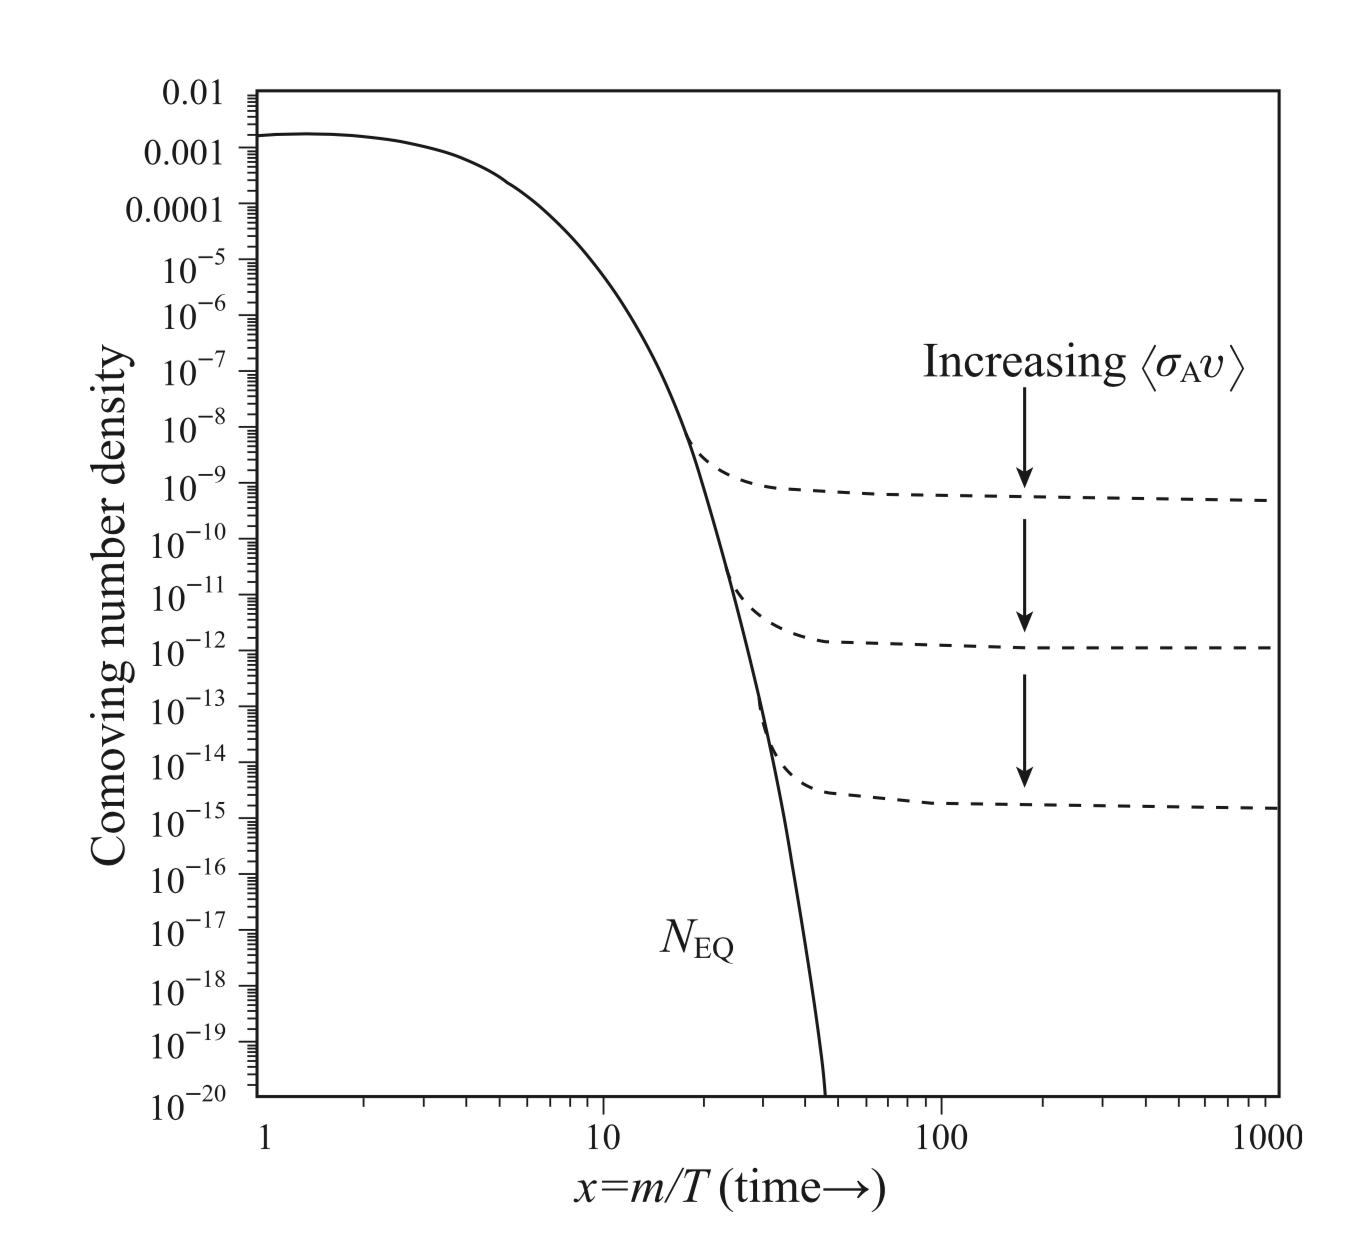
\includegraphics[width=0.6\textwidth]{figs/WIMP_thermal_relic}
  \caption{The WIMP comoving number density as a function of time, also parametrized as $x_f = \frac{\mDM}{T_f}$, where an increase in the annihilation cross section ultimately results in a later freeze-out time, and a correspondingly lower thermal relic density~\cite{Kolb:1990vq}.}
  \label{fig:WIMPrelic}
\end{figure}

Thus, yielding a naturally correct $\Omega_\chi$ via the freeze-out production mechanism, and characterized by the kinematic qualities of CDM which predict the structure formation observed in the Universe today, the WIMP is the most theoretically preferred DM candidate. WIMPs are predicted by many BSM theories, whether as neutralinos in supersymmetric (SUSY) theories, super-heavy and super-weakly-interacting particles coupling to SM fields via the Higgs portal called WIMPzillas, or through effective field theory operators (EFT) which describe the weak contact interaction between SM particles and DM. In short, the WIMP provides model-independent grounds for weak scale DM production, which furthermore allows the experimental community to search for its existence via multiple independent and complementary methods.

\section{Dark matter detection}
\label{sec:DMsearches}

Favorable implications for DM detection arise as a result of the WIMP miracle. In order to reach the correct relic density, the WIMP DM particles must also annhilate to other particles, which are assumed to be SM particles. The process of $\chi \bar{\chi} \rightarrow \mathrm{SM}\:\mathrm{SM}$ means it is possible to write down the elastic scattering and annihilation cross sections of DM and ordinary particles within a framework of a particle physics theory. It has been established that DM is responsible in part for the dynamics of galaxies and clusters, which in turn lead to the large scale structures observed today. The galactic halo of our own Milky Way galaxy is predicted to be abundantly filled with DM particles, and the WIMP model would allow for the detection of signals emitted by DM annihilation to SM particles. Conversely, the stability and proliferation of WIMPs would allow DM particles to reach terrestrial laboratories, where a potential DM signal would reveal itself as elastic scattering of DM off ordinary particles depositing energy in sensitive detectors. By construction, the WIMP paradigm would also allow for the reversal of the annihiliation process, such that the production of pairs of DM particles from extremely highly energetic SM particles is possible. The annihilation, elastic scattering, and production of DM are the underlying strategies respectively used by indirect, direct, and collider methods of DM detection detailed in this section.

\subsection{Indirect detection}
\label{subsec:ID}

Although DM makes up a substantial part of the Universe, it nonetheless, does not constitute the entirety of the energy-mass density ratio, thus the observed $\Omega_\chi$ was reached through its annihilation. The WIMP miracle implies that DM-SM interactions must be efficient, thus if DM annihilation occured during the early Universe, it must also proceed in the same way today albeit at a lower frequency, making it possible to detect the SM products from the reaction. Indirect searches for DM target a large region of the cosmos, such as the sun, the galactic halo of the Milky Way and that of other galaxies. An indirect detection (ID) signal would typically manifest itself as an anomalous event of cosmic rays, where DM annihilation results in an abnormally high rate of SM particle-anti-particle pair production. Fluxes of cosmic rays can encompass a large number of particles though most ID experiments focus on signatures of charged particles ($e^- e^+$, $p \bar{p}$, deuterium and antideuterium), photons (in the form of gamma rays, X-rays, or synchrotron radiation), and lastly, neutrinos. Experiments dedicated to searches of charged anti-particle fluxes make good use of the under-abundance of anti-particles with respect to their corresponding particles in the Universe, whereas dedicated photon and neutrino flux experiments target areas of the cosmos that can maximize the potential DM signal to noise from astrophysical sources. The cosmic fluxes of the aforementioned elementary particles are a result of the showering and hadronization of the pair-produced primary particles from the DM annihilation, such as $b\bar{b}$, $\mu^+\mu^-$, $\tau^+\tau^-$, and $W^+W^-$. The spectra of the cosmic rays depends in large part on the mass of the primary particles that emmitted the flux, but in general the distribution features a 'bump'-like structure which is characterized by a high-energy cutoff at the \mDM. 

\begin{figure}
  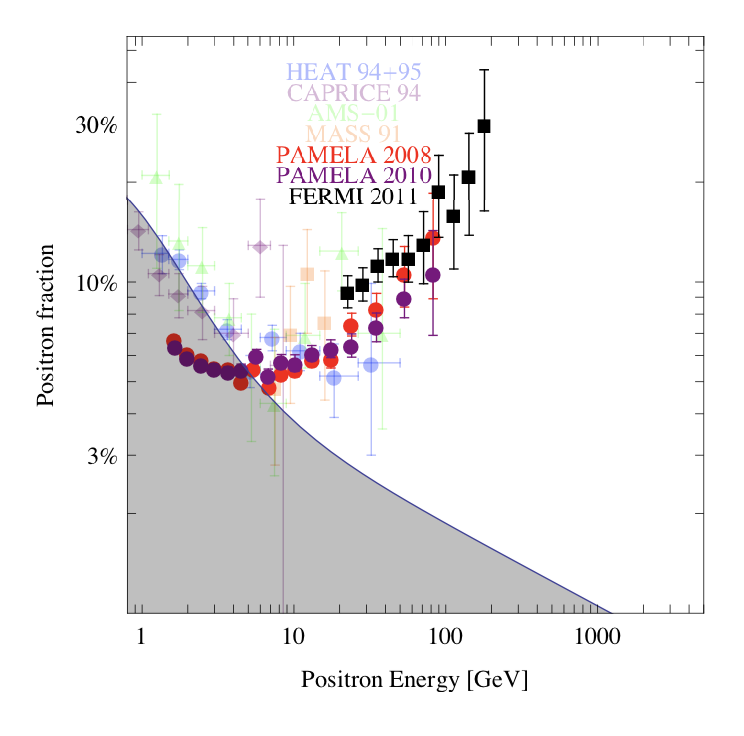
\includegraphics[width=0.7\textwidth]{figs/pamela.png}
  \caption{The positron energy spectra measured by a compilation of recent (PAMELA and FERMI) and less recent ID experiments dedicated to measurements of secondary charged particles emmitted in cosmic ray fluxes. The data is superimposed on a compilation of uncertain astrophysical backgrounds from secondary production.~\cite{Cirelli:2012tf}}
  \label{fig:positronflux}
\end{figure}

Myriad ID experiments are currently under operation or are projected for future searches. An example of one such experiment is the PAMELA satellite~\cite{Adriani:2008zr} which presented an excess over a potential but uncertain background from secondary astrophysical sources in the positron energy spectra for $10\:\GeV < E_{e^+} < 100\:\GeV$, as seen in~\FigureRef{fig:positronflux}. The excess was also extended to $200\:\GeV$ and confirmed independently by measurements from the FERMI satellite~\cite{PhysRevLett.108.011103}, and the prototype Alpha Magnetic Spectromenter (AMS-01) experiment~\cite{Aguilar:2007yf}. Although the signals seem quite striking since it implies a source of $e^+$ exists other than ordinary astrophysical ones, it is precisely the uncertainties in these backgrounds and their potentially exotic contributions to the spectra that limit the interpretation of ID signals as DM. In this respect, not only are other ID experiments necessary to confirm a signal as a potential DM discovery, but another means of detection altogether is required to corroborate a signal from indirect detection methods, since improving the simulation and understanding of astrophysical backgrounds is non-trivial.

\subsection{Direct detection}
\label{subsec:DD}

The non-relativistic nature of the WIMP would allow for its detection via elastic scattering off a SM particle, which imparts a transfer of momentum to the nucleus, known as the nuclear recoil. Direct detection (DD) experiments are sensitive to the secondary effect of the nuclear recoil and thus detect a potential WIMP signature through the light, heat, or ionization of the SM material with which it interacted. DD experiments are typically conducted in deep, underground terrestrial laboratories in order to suppress the highly energized neutron fluxes produced from cosmic rays that penetrate the atmosphere, since such backgrounds are the most serious and challenging to disentangle from a potential signal. A sufficient amount of Earth material or water/ice is necessary to shield the highly sensitive detectors and reduce the high cosmic muon intensity fluxes. Furthermore, as a result of the small interaction rate of DM-SM particles, DD experiments observe single interactions as opposed to multiple interactions, and it thus follows that any interactions would be uniformly distributed within the detector volume, contrasting the background from radioactivity expected at the detector surface.

The formalism of WIMP DD is summarized in the following steps, where more details are given in \cite{Jungman:1995df}:

\begin{itemize}
\item The kinetic energy of a recoiled nucleus, after elastic scattering is approximately,

\begin{equation}
  E_{r} \approx (\frac{1}{2}\mDM v^2)\Big(\frac{4\mDM m_N}{(\mDM + m_N)^2}\Big)\cos^2{\theta_R},
  \label{eq:kinE}
\end{equation}

where $\theta_R$ is the angle of nuclear recoil, $m_N$ is the mass of the nucleus, and $v$ is the velocity of $\chi$ relative to the detector in question. With an expected WIMP local density in the Milky Way galactic halo of $\rho_{\chi 0}=0.4\:\GeV/c^2/cm^3$, $v^2$ is approximately $\mathcal{O}(10^{-6})$ at the average detector depth, and \EquationRef{eq:kinE} is maximized to a value of $10^{-6}\mDM$ when the DM and nucleus mass are equal. Thus a WIMP mass on the order of $100\:\GeV$ would lead to $E_r \approx 0-100\:\mathrm{keV}$.

\item The detection rate depends on the reaction cross section of the DM and the SM nucleus collision, which can be parametrized as a function of the nuclear momentum transfer $q_r = 2m_rv\cos\theta_r$, where $m_r$ is the reduced mass of the $\chi-N$ system. The parametrization leads to a differential cross section of a recoiled nucleus,

\begin{equation}
  \frac{\mathrm{d}\sigma(q_r)}{\mathrm{d} q_r^2} = \frac{\sigma_0}{(2m_r v)^2}F^2(q_r),
\label{eq:diffxsec}
\end{equation}

where the denominator on the right-hand side of \EquationRef{eq:diffxsec} is the square of the maximal momentum transfer that occurs for forward scattering. The form factor, $F(q_r)$, accounts for the finite size of the nucleus and can depend on whether the DM-SM interaction is spin-independent (SI) or spin-dependent (SD). In addition, the total recoil cross section, $\sigma_0$, has SI and SD contributions, where the $\sigma_{SI}$ depends on the couplings of the WIMP to protons and neutrons in the given model, though generically they are expected to be equal.

\item The interaction rate per unit detector mass in a given velocity range $[v,v+dv]$ goes as,

\begin{equation}
  dR = \Big(\frac{\rho_{\chi 0}}{m_\chi m_N}\Big) v \frac{\mathrm{d}\sigma(q_r)}{\mathrm{d} q_r^2} f_1(v)\mathrm{d}v\mathrm{d}q_r^2
\label{eq:DDrate}
\end{equation}

where the $f_1(v)$ is a Maxwellian distribution that models the galactic WIMP velocity. 

\item The velocity integration in \EquationRef{eq:DDrate} gives the rate as a function of the recoil energy from \EquationRef{eq:kinE} and yields,

\begin{equation}
  \frac{dR}{dE_r} \propto \exp{\Big(\frac{-m_N E_r}{2m_r^2v_0^2}\Big)}.
\end{equation}

Thus, in contrast to the expected peak structure that would be observed by ID experiments, the recoil spectrum that DD experiments look for is approximately described by an exponential. For this reason, there is no precise spectral signature, and most of the signal is expected to lie at the low recoil energy range requiring a firm understanding of the experimental energy thresholds of dedicated WIMP direct detectors.
\end{itemize}

Unlike ID experiments, DD experiments may make some assumption on the particle physics model which dictates the values of $\sigma_0$ and $F(q_r)$ ultimately changing the interaction rate expected in a given type of detector material. Taking the example of a neutralino ($\tilde{\chi}^0$) from SUSY models as the WIMP candidate, the $\tilde{\chi}^0$-nucleon cross section depends on the coupling between the $\tilde{\chi}^0$ and quarks in the low-energy regime. These interactions are mediated through scalar, pseudoscalar, axial, and axial-vector currents, in the same manner that electroweak interactions are mediated via gauge $vector$ bosons. In particular, the $\tilde{\chi}^0$ is a Majorana fermion~\cite{Majorana2006}, and thus can only couple to the particles in the SM sector via scalar or axial-vector currents. Axial-vector and pseudoscalar couplings give rise to SD WIMP-nucleon cross sections, while vector and scalar couplings generate SI cross sections.

The most sensitive SI DD searches make use of low-temperature heat and ionization detectors, or consist of dual-phase noble liquids. Since the SI cross section is directly proportional to the target nucleus mass, such detectors employ heavy nuclei such as xenon (Xe) and germanium (Ge). An example of one such experiment is the XENON1T experiment~\cite{refId0}, which makes use of liquid Xe (LXe) time projection chambers (TPCs). Located at a depth of 3600 m at the INFN Laboratori Nazionali del Gran Sasso (LNGS), 2 t of ultra-pure LXe serves as the active target material in the detector which produces prompt scintillation (S1) once a particle is incident upon the target LXe nucleus. Secondary electron ionization is also produced from the energy deposit and once the electrons pass through the drift field, they are extracted into gaseous Xe (GXe) where they produce proportional scintillation light (S2). The XENON1T experiment utilizes the ratio S2/S1 to discriminate between nuclear recoils produced by WIMP or neutron interactions and electronic recoil from $\beta$ or $\gamma$ interactions. The results from the XENON1T experiment improve upon the those from PandaX-II~\cite{PhysRevLett.119.181302} and LUX~\cite{PhysRevLett.118.021303}, both technologically similar experiments. As shown in~\FigureRef{fig:xenon1t}, the recent XENON1T results exclude WIMP-nucleon $\sigma_{SI}$ of $\mathcal{O}(10^{-46})\:\mathrm{cm}^2$ for $\mDM \approx 20-30\:\GeV$, and demonstrate a seven-fold improvement in sensitivity over PandaX-II and LUX for $\mDM > 50\:\GeV$ as seen in the inset by the limits normalized to the median of the XENON1T sensitivity. Over the past several decades, the detector volume of DD experiments has expanded with the aim of increasing the sensitivity by maximal exposure. The XENON1T experiment is projected to be superceded by XENONnT, an 8 t detector predicted to reach a $\sigma_{SI}$ limit of $1.6\times10^{-48}\:\mathrm{cm}^2$ for $\mDM\approx 50\:\GeV$~\cite{2017APS..APR.J9003A}.

\begin{figure}
  \centering
  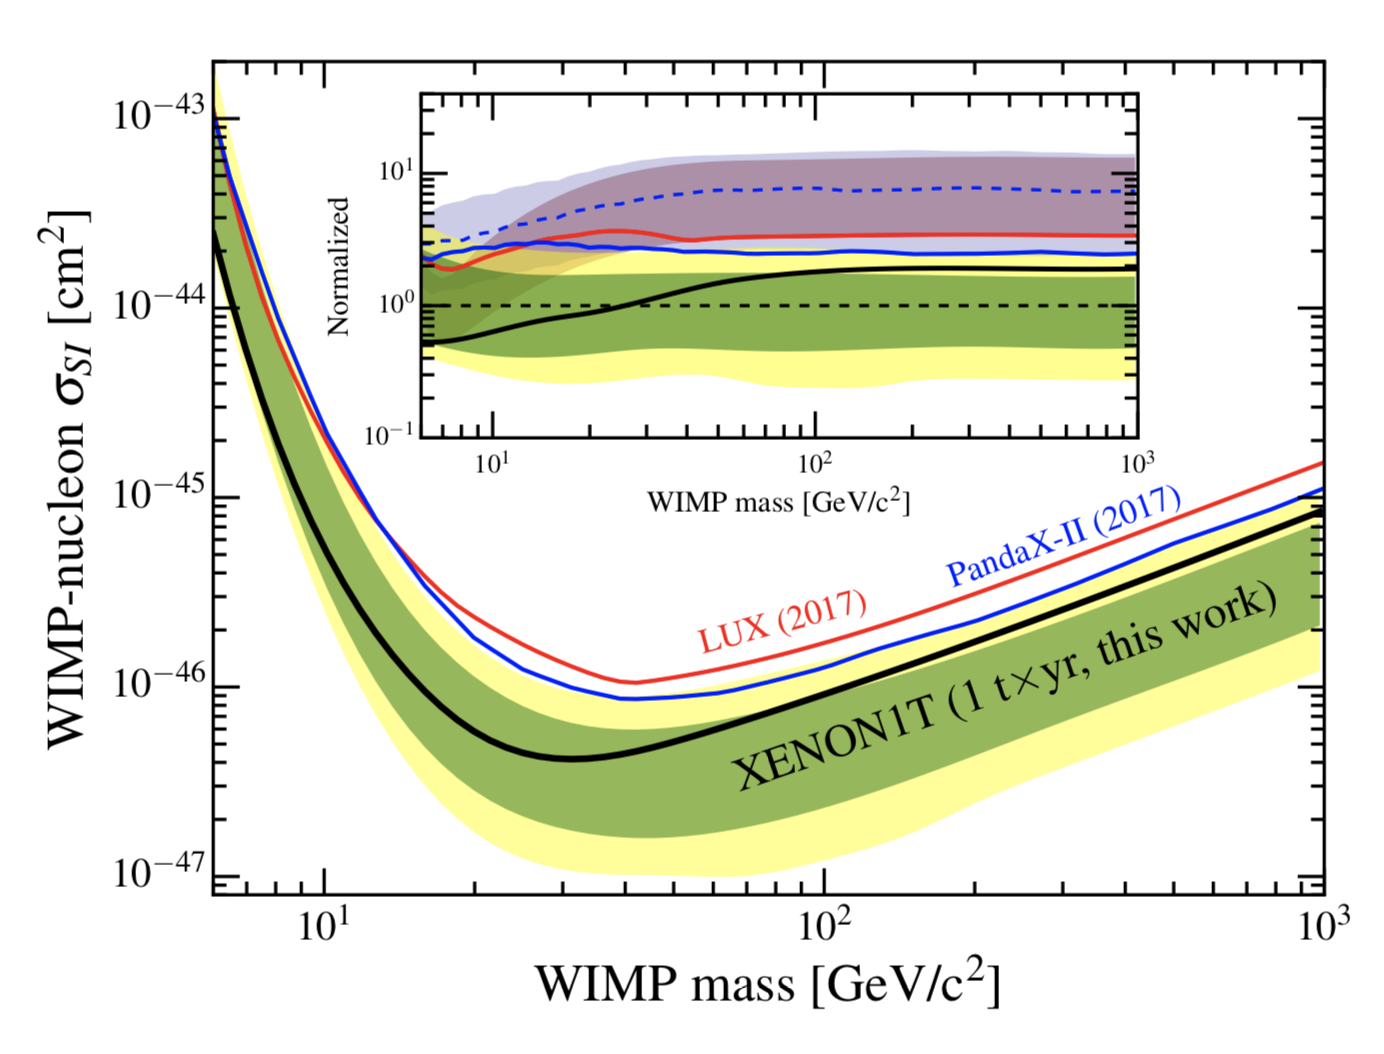
\includegraphics[width=0.7\textwidth]{figs/Xenon1T}
  \caption{Cross section limits as a function of the DM mass for spin-independent interactions for PandaX-II, LUX, and XENON1T.}
  \label{fig:xenon1t}
\end{figure}

The SD DD experiments are instead strongly reliant on the spin content of the target nucleus, and essentially translate to a constraint on the WIMP coupling coefficients to protons, $a_p$, or neutrons, $a_n$ which affect the form factor in \EquationRef{eq:diffxsec}. These experiments can also employ dual-phase noble gas TPCs, or solid scintillators and superheated bubble chambers to achieve high sensitivities at high and low \mDM, respectively. At present, the strongest constraints to SD WIMP-proton interactions are given by thermodynamically operated superheated detectors containing fluorine-rich liquids. Filled with approximately 52 kg of $\mathrm{C}_3\mathrm{F}_8$ target and operated at SNOLAB in Sudbury, Canada, the PICO-60 bubble chamber sets the most stringent constraints on the WIMP-proton $\sigma_{SD}$ at $3.4\times 10^{-41} \mathrm{cm}^2$ for $\mDM=30\:\GeV$~\cite{Amole:2017dex}.
 
\subsection{Collider searches}
\label{subsec:Collider}

As is the case with direct DM detection, searches for DM production at colliders also take into account the possible particle nature of DM, allowing in many cases for a comparison between these two vastly differing search strategies. In order to emulate the high temperature environment of the early Universe during which WIMPs are postulated to have been produced, the energy of the colliding SM particles at accelerators is necessarily very high. The accelerated particles are typically extremely light, such as protons, anti-protons, electrons or positrons, allowing for their collision energy to be maximized. As a result, collider searches are particularly sensitive to very low WIMP masses on $\mathcal{O}(\GeV)$. However, if DM is much heavier than the $\mathcal{O}(\TeV)$ scale, it may be the case that the center-of-mass energy available at present collider experiments is insufficient to kinematically allow for the production of DM. Even if DM is produced promptly within the detecting volume at a collider, the further complication for these searches is the lack of experimental signature. DM particles would not interact with the detector material and only reveal their presence through an imbalance of total transverse momentum, also known as missing transverse energy (\MET). This quantity, described in detail in \SectionRef{sec:MET}, can be understood as the application of the laws of conservation of energy and conservation of momentum to a collision to infer the presence of a weakly interacting particles. SM neutrinos manifest as \MET in a detector because of their extremely weak interactions with the material. The saving grace of collider searches is that SM particles are predicted to be produced in conjunction with the DM particles by a plethora of relevant particle physics models. The experimental feasibilty is therefore increased for such searches, since the differential distributions of SM background processes are sufficiently well-understood, that even minute deviations from the expected \MET spectrum would allow for the constraint of DM models predicting such signals. The following section will explore the physics model context in which WIMPs are produced and collider searches are interpreted by this work.

\section{Simplified models of DM: beyond the Standard Model}
\label{sec:BSM}

As mentioned earlier, the production of DM within different types of BSM particle physics models probed by collider searches allows for the detection of a potential signal indirectly via the SM particles that are expected to be produced in association with the WIMPs. Such searches performed by the ATLAS and CMS collaborations are termed $\text{Mono}$-$X$ searches, where the $X$ is the SM particle(s) produced together with the DM particles. The models which the searches in question target, are numerous and span a range of completeness. Supersymmetric (SUSY) extensions to the SM are amongst the most complete BSM theories, and correspondingly incur the largest number of model parameters. SUSY models also do not necessarily directly tie together the annhilation of SM particles to the production of DM particles, since the DM particles are often secondarily produced together with a significant number of SM particles. The constraints that exist for SUSY models are also, in large part, not related to the DM particle itself, but apply to a greater degree to the other parameters. In favor of a simpler description of the DM-SM interactions, a class of models characterized by fewer tuneable parameters, albeit less theoretically complete, are investigated in this work. 

DM production at colliders can be described, in large part, by the interaction between the SM and DM particles. Prior to Run II of the LHC, DM searches such as the one detailed in~\cite{Khachatryan:2016reg}, had been traditionally interpreted using Effective Field Theory (EFT) models~\cite{Goodman:2010ku}, wherein the interaction between the SM particles and the Dirac fermion WIMPs is mediated through higher dimensional operators. The models are solely characterized by \mDM, and $M_{*}$ which represents the strength of the interaction and is a function of the masses and coupling strengths of the mediating particles between the DM and SM fields. The benefit of the EFT formulation is the lesser degree of model dependence, and the relative ease encountered in translating experimental collider constraints to the direct detection DM-nucleon cross section-\mDM plane. The shortcoming of such field theories, however, are that they are non-renormalizable, thus they become invalid at arbitrarily high energy scales. This is represented by the masses of the mediating particles that have been integrated out. In general, for an EFT to make sense, it is required that $M_{*}$ be much larger than the energy transfer through quarks at the LHC, $M_{*}^{2} \gg Q_{\textrm{tr}}^{2}$. Put another way, the EFT formalism is valid only if the energy scale of the interaction involving the DM and the SM particles is small with respect to the energy scale associated to the heavy mediator, $M_{*}$. In general, ID and DD experiments adhere to this requirement since the expected energy transfers are of the order of \mDM or $\mathcal{O}(\mathrm{keV})$, respectively. In the high energy environment of collider searches, however, the processes that might be described by the EFT operators would occur in a region beyond the validity of the theory~\cite{BUSONI2014412}. Thus, since this class of models does not truly account for the mediator, effects from resonant enhancement are not included and EFTs have no description of off-shell mediator production.

In order to circumvent the deficiencies of the EFT formalism, a class of \textit{simplified models} have been employed for the interpretation of DM searches during Run II of the LHC. In part, the increase in the center-of-mass collision energy from $\sqrt{s}=8\:\TeV$ to $\sqrt{s}=13\:\TeV$ further limits the region of validity for the EFT models. Hence, the contact interaction of the EFT models, as depicted in~\FigureRef{subfig:EFT}, is subsequently resolved into a mediator interaction which couples to the SM and DM particles, as shown in~\FigureRef{subfig:DMsimp}, thus increasing the free parameters to include the coupling of the mediator to the SM sector, \gq, the coupling of the mediator to the DM sector, \gDM, the mass of the mediator, \mMed, and \mDM. For comparison,~\FigureRef{subfig:SUSY} shows a SUSY model of sgluon-mediated ($\tilde{g}$), di-squark ($\tilde{q}$) decay to SM particles and $\tilde{\chi}^0$s.\FigureRef{subfig:DMsimp} is called a simplified model of DM and in particular, the Feynman diagram represents a spin-1 s-channel mediated process where at least one SM particle from initial state radiation and a $\chi\bar{\chi}$ pair is expected.

\begin{figure}
  \subfloat[][EFT model]{\label{subfig:EFT} 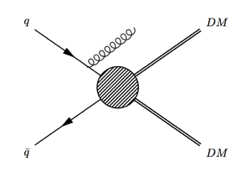
\includegraphics[width=0.3\textwidth]{figs/MJ_EFT}}
  \subfloat[][Simplified model of DM]{\label{subfig:DMsimp} 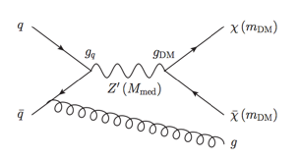
\includegraphics[width=0.3\textwidth]{figs/MJ_DMSimp}}
  \subfloat[][SUSY model]{\label{subfig:SUSY} 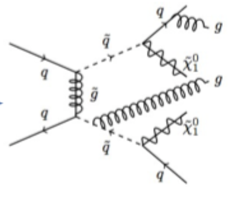
\includegraphics[width=0.3\textwidth]{figs/SUSY}}
\caption{}
\label{fig:models}
\end{figure}

Simplified DM models are built upon three major criteria:

\begin{itemize}
  \item The DM particle must be absolutely stable or else have a lifetime long enough to escape the LHC detectors
  \item The Lagrangian should contain renormalizable terms which are also Lorentz invariant, obey the SM gauge symmetries and give stable DM
  \item Additional interactions between the DM and SM sector must conserve baryon and lepton number and only break custodial and flavor symmetries softly~\cite{Abdallah:2015ter}
\end{itemize}

The third criterion is met by the assumption of Minimal Flavor Violation (MFV)~\cite{PhysRevLett.65.2939} which curbs flavor and $\mathcal{CP}$-violation in models of new physics. The essential idea behind MFV is that new physics must preserve the general structure of flavor-changing neutral current (FCNC) processes present in the SM. Thus, any flavor and $\mathcal{CP}$-violating transitions are entirely dictated by the CKM matrix. In particular, this work is focused on the minimally flavor violating spin-0 models, where it is shown in \cite{Abdallah:2015ter} that through MFV the $s$-channel couplings of the SM fermions to the DM sector are required to be of Yukawa type. The interaction Lagrangians of the spin-0 scalar ($\phi$) and pseudoscalar ($a$) mediators are as follows~\cite{Abercrombie:2015wmb},

\begin{equation}
  \mathcal{L}_{\phi} = g_{\chi}\phi\chi\bar{\chi} + \frac{\phi}{\sqrt{2}}\sum_{i}{(g_{u}y_{i}^{u}\bar{u}_{i}u_{i} + g_{d}y_{i}^{d}\bar{d}_{i}d_{i} + g_{\ell}y_{i}^{\ell}\bar{\ell}_{i}\ell_{i})},\\
  \mathcal{L}_{a} = ig_{\chi}a\chi\gamma_{5}\bar{\chi} + \frac{ia}{\sqrt{2}}\sum_{i}{(g_{u}y_{i}^{u}\bar{u}_{i}\gamma_{5}u_{i} + g_{d}y_{i}^{d}\bar{d}_{i}\gamma_{5}d_{i} + g_{\ell}y_{i}^{\ell}\bar{\ell}_{i}\gamma_{5}\ell_{i})}
\end{equation}

where the Yukawa couplings are $y_{i}^{f} = \sqrt{2}m_{i}^{f}/v$, where $m^{f}_{i}$ is the fermion mass, and $v=246\:\GeV$ is the Higgs boson field vacuum expectation value. $g_{u}, g_{d}$ and $g_{\ell}$ represent the coupling strength between the mediator and up-type quarks, down-type quarks, and leptons respectively. In the report issued by the Dark Matter Forum (DMF)~\cite{Abercrombie:2015wmb}, a collaboration between members of CMS, ATLAS and the theory community, a benchmark set of parameters for the relevant simplified models of DM were chosen after scans of the parameter space were performed. In the following work, the DMF recommendation of $\gDM = g_{u} = g_{d} = g_{\ell} = 1$ has been adopted. This reduces the free parameters to \{\mDM, \mMed\} which contribute to the minimal mediator width at leading order (LO) via, 

\begin{equation}
  \Gamma_{\phi} = \frac{\mDM}{8\pi}\Big(1-\frac{4\mDM^{2}}{m_{\phi}^2}\Big)^{x/2} + \sum_{f=fermions}\frac{y_{f}^{2}m_\phi}{16\pi}\Big(1 - \frac{4m_{f}^2}{m_{\phi}^2}\Big)^{x/2},
  \label{eq:width}
\end{equation}

with $x=3$ for scalar mediators, and $x=1$ for pseudoscalar mediators. Owing to the choice of SM Higgs-like Yukawa couplings for the SM fermions, the top quark contribution to the mediator width is enhanced at mediator masses above twice the top quark mass, but conversely for lighter mediator masses, the DM contribution dominates since couplings to the lighter quarks are Yukawa-suppressed. In addition, since the Yukawa-type coupling of the spin-0 mediator to the SM favors the more massive of the fermion generations, this strongly motivates searching for DM produced in association with heavy flavor quarks, such as top quarks. The standard EFT diagram characterizing \ttDM production is shown in~\FigureRef{fig:EFT}, while the simplified model investigated in this work can be seen in~\FigureRef{fig:DMF}.

\begin{figure}
  \subfloat[][]{\label{fig:EFT}
    \feynmandiagram[vertical=b to d]{
      a [particle=\(\bar{t}\)] -- [fermion] b -- [fermion] c -- [fermion] d -- [fermion] e [particle=\(t\)],
      f [particle=\(g\)] -- [gluon] b,
      g [particle=\(g\)] -- [gluon] d,
      h [particle=\(\bar{\chi}\)] -- [fermion] c -- [fermion] i [particle=\(\chi\)],
      h -- [opacity=0.001] i,
      %%f -- [opacity=0.001] g,
      a -- [opacity=0.001] h,
      e -- [opacity=0.001] i,
    };
  }
  \hspace{0.5cm}
  \subfloat[][]{\label{fig:DMF}
    \feynmandiagram[horizontal=c to h]{
      a [particle=\(\bar{t}\)] -- [fermion] b -- [fermion] c -- [fermion] d -- [fermion] e [particle=\(t\)],
      f [particle=\(g\)] -- [gluon] b,
      g [particle=\(g\)] -- [gluon] d,
      c -- [scalar, edge label=\(\phi \slash a\)] h,
      i [particle=\(\bar{\chi}\)] -- [fermion] h -- [fermion] j [particle=\(\chi\)],
      e -- [opacity=0.0001] i,
      a -- [opacity=0.0001] j,
      i -- [opacity=0.0001] j,
      %%      f -- [opacity=0.0001] g,
    };
  }
  \caption{The representative diagram of a top quark pair produced in association with a pair of DM particles ($\chi\bar{\chi}$) using~\protect\subref{fig:EFT} the EFT formalism and~\protect\subref{fig:DMF} the simplified model formalism.}
\end{figure}

  \chapter{The \CMS experiment}
\label{chap:CMS}

%\chapterquote{There, sir! that is the perfection of vessels!}
%{Jules Verne, 1828--1905}

\section{The \LHC}
The Large Hadron Collider (\LHC) at \CERN is the most powerful particle accelerator in the world, located in the same tunnel as the Large Electron-Positron collider (\LEP)~\cite{Brianti:2004qq}. The mandate of the \LHC experimental program is two-fold: to probe the electroweak symmetry breaking mechanism via which particles in the Standard Model (SM) attain mass, and to extend the exploration of the energy frontier in search for new physics beyond the SM (\BSM).

\section{The \CMS experiment}
\label{sec:CMSInDetail}

The CMS detector, described in detail in Ref.~\cite{CMS}, is a multi-purpose apparatus designed to study high-\pt physics processes in proton-proton and heavy-ion collisions. A superconducting solenoid in its central region provides a magnetic field of 3.8 T parallel to the beam direction. Charged particle trajectories are measured by silicon pixel and strip trackers, which cover a pseudorapidity region of $|\eta| < 2.5$. Surrounding the tracker volume are a lead-tungstate crystal electromagnetic calorimeter (ECAL) and a brass-and-scintillator hadron calorimeter (HCAL) surround the tracking volume, covering the region of $|\eta| < 3$. A steel and quartz-fiber Cherenkov forward hadron calorimeter extends the coverage to $|\eta| < 5$. The muon system consists of gas-ionization detectors embedded in the steel flux return yoke outside the solenoid, and covers the region with $|\eta| < 2.4$. The detector is designed to cover a 4$\pi$ solid angle. The detector is illustrated in \FigureRef{fig:CMSCrossSection}, showing the overall scale of the experiment and the surrounding cavern structure.

\vspace{1cm}

The first level of the CMS trigger system is composed of custom hardware processors and designed to select the most interesting events in less than 4 $\mu\text{s}$, using information from the calorimeters and muon detectors. This system reduces the event rate from 40 MHz to approximately 100 kHz.  The high-level trigger processor farm performs a coarse reconstruction of events selected by the first-level trigger, and applies additional selections to reduce the event rate to about 1 kHz for storage.

\vspace{1cm}

One of the main mandates of the CMS detector is to provide good resolution and reconstruction efficiency for charged particles emmitted from LHC collisions in the inner tracker. Furthermore, the precise reconstruction of secondary vertices is imperative for the efficient identification of b-jets; b-jets being the only flavor jets expected in the dilepton channel \ttDM signal final state topology. To achieve this, it is imperative for the positioning of tracker layers to be close to the interaction point of a collision, hence the first and last of the three pixel barrel layers are stationed at radii 4.4 cm to 10.4 cm. What follows these layers, are the four and six silicon strip layers comprising the Tracker Inner Barrel (TIB), and Tracker Outer Barrel (TOB), respectively. The last TOB layer reaches an outward radius of 1.1 m from the beampipe. The barrel layers of both the pixel and strip systems are complimented by disk layers on either +/-z position of the interaction point. There are two pixel disks on either side of the barrel layer, while there are three small disks and nine larger disks, known as the Tracker Inner Disks (TID) and Tracker EndCaps (TEC) respectively, which flank the strip barrel layers. A cross-sectional view of the tracker can be seen in \FigureRef{fig:trackerxsec}. 
 

\begin{sidewaysfigure}
  \begin{center}
  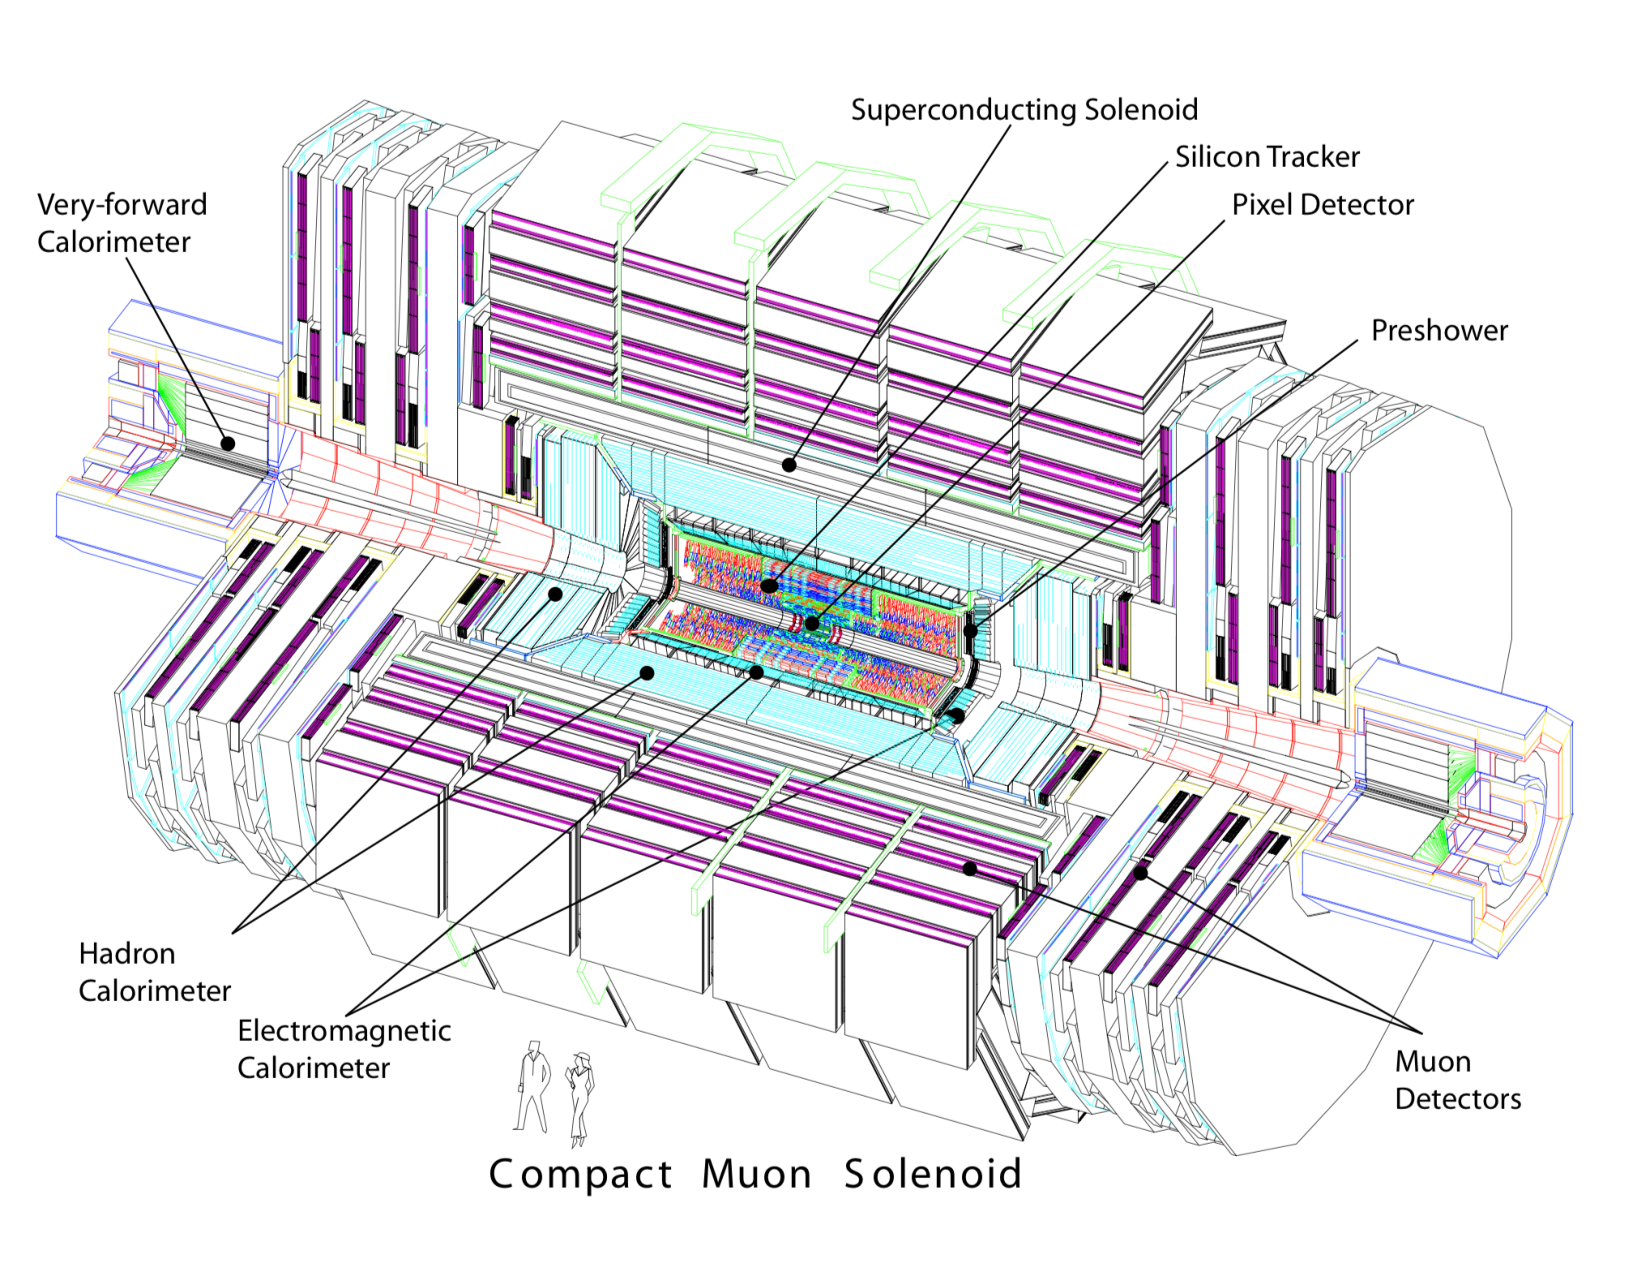
\includegraphics[width=0.8\textheight]{figs/CMScrosssection.pdf}
  \caption[Cross-section view of \CMS]%
    {Cross-section view of \CMS.}
  \label{fig:CMSCrossSection}
  \end{center}
\end{sidewaysfigure}

\begin{figure}
  \begin{center}
    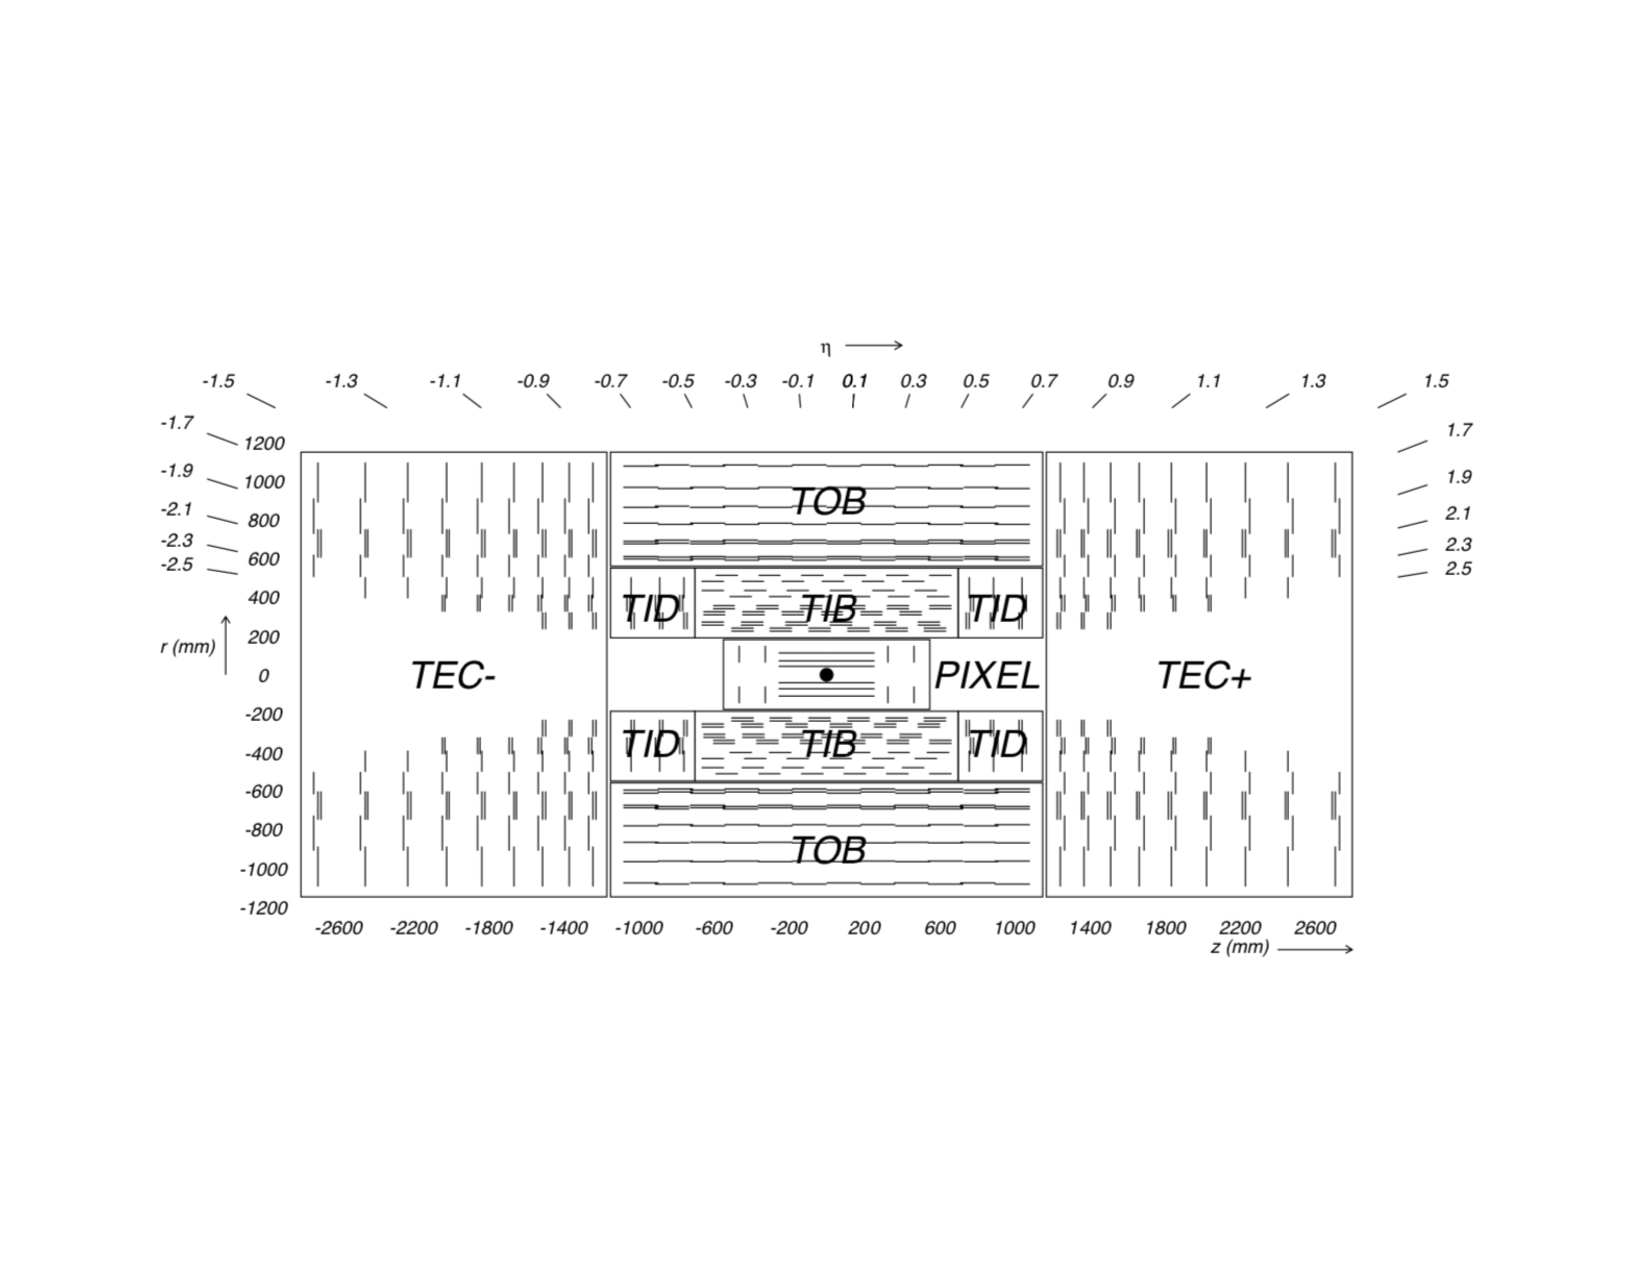
\includegraphics[width=\textwidth]{figs/tracker_schematic.pdf}
    \caption[Schematic cross-section through the \CMS tracker, where a single detector modules is represented by a line, and double lines signify back-to-back modules.]{Schematic cross-section through the \CMS tracker, where a single detector modules is represented by a line, and double lines signify back-to-back modules.}
    \label{fig:trackerxsec}
  \end{center}
\end{figure}

%The single-sided detector design was chosen in preference to a two-armed
%design since the detector dimensions are restricted by the layout of the
%IP8 (ex-Delphi) cavern in which \LHCb is located. Using all the available
%space for a single-arm spectrometer more than compensates in performance
%for the \about{50\percent} drop in luminosity.

%\section{The \Cerenkov mechanism}
%A Huygens construction in terms of spherical shells of probability for photon
%emission as the particle progresses along its track shows an effective
%``shock-front'' of \Cerenkov emission. This corresponds to an emission cone of
%opening angle \thetaCerenkov around the momentum vector for each point on the
%track,
%%
%\begin{subequations}
%  \label{eq:cosThetaCk}
%  \begin{equation}
%    \cos\,\thetaCerenkov  &= \frac{1}{n \beta} +
%                             \frac{\hbar k}{2p}%
%                             \parenths{ 1 - \frac{1}{n^2} } \\
%                          &\,\sim \frac{1}{n \beta}%
%    \label{eq:cosThetaCkApprox}
%  \end{equation}
%\end{subequations}
%
%where $\beta \equiv v/c$, the relativistic velocity fraction.

%\section{Trigger system}
%\label{sec:triggers}
%An overview of the \LHCb trigger characteristics broken down by level
%is shown in \Table~\ref{tab:TriggerDetails}.

%\begin{table}[bp]
%  \begin{tabular}{lllll}
%                & L0              & L1              & HLT             \\
%    \midrule\\
%    Input rate  & \unit{40}{\MHz} & \unit{1}{\MHz}  & \unit{40}{\kHz} \\
%    Output rate & \unit{1}{\MHz}  & \unit{40}{\kHz} & \unit{2}{\kHz}  \\
%    Location    & On detector     & Counting room   & Counting room   \\
%  \end{tabular}
%  \caption{Characteristics of the trigger levels and offline analysis.}
%  \label{tab:TriggerDetails}
%\end{table}

  \chapter{Object and event reconstruction}
\label{chap:eventreco}

In order to target \ttDM production in the dilepton final state, where both top quarks have leptonically decaying W bosons, the selection criteria is compatible with that of SM \ttll decays, but with a requirement targetting the harder \MET spectra as expected from signals compared to the SM background.

Owing to the design elements of the CMS detector as described in \ChapterRef{chap:CMS}, it has been found that it is well-suited to particle-flow (PF) reconstruction of physics objects, expanded upon in \SectionRef{sec:PF}, from the signals collected by each subdetector. \SectionRef{sec:leps}-\ref{sec:MET} detail the means by which the PF quantities are employed in the reconstruction of particular objects, and the criteria each object in an event must adhere to in order to be considered a potential signal event. \SectionRef{sec:selection} explains how the reconstructed event objects are used collectively, to target a region where a \ttllDM signal is expected.

\section{The Particle Flow algorithm}
\label{sec:PF}

A key feature of the CMS detector which allows for the correlation of signals from different sources is the fine spatial granularity and segmentation of the individual constituent subdetectors. As a result of the fine-grain tracker and strong magnetic field, very efficient charged-particle track reconstruction is possible, which accounts for $\sim 65\%$ of jet energy measurement. Additionally, the high ECAL segmentation provides the ability to separate energy deposits from particles in jets from one another, allowing for the efficient identification of photons and the measurement of $\sim 25\%$ of the jet energy. The remaining $\sim 10\%$ of the jet energy measurement comes from the HCAL, which has a sufficient segmentation to allow for the separation of charged and neutral hadron energy deposits from particles in jets. Lastly, as per its namesake, the CMS detector has an excellent muon system enabling pure and efficient muon identification regardless of the surrounding particles.

The goal of the PF algorithm is thus to optimally combine the information from the aforementioned subdetectors, which is done via the following simplified description, where more details can be found in~\cite{Sirunyan:2017ulk}:
\begin{itemize}
  \item Tracks from the pixel and strip tracker are extrapolated through the calorimeters (``inside-out'').
  \item If the tracks land within certain spatial boundary requirements of one or several clusters, they are linked to the track in question resulting in a charged hadron candidate. This PF candidate is subsequently not considered in the remainder of the algorithm.
  \item By this point, muons have been independently identified by a correlation of hits between the tracker and the muon system detectors, thus removing any potential ambiguity of track association to muons or charged hadrons.
  \item The treatment of electrons is complicated by the fact that frequent Bremsstrahlung gives rise to multiple possible energy clusters that can be associated to a track, thus dedicated track reconstruction is required to properly match ECAL clusters from the emitted photons to the electron track. 
  \item Finally, the remaining ECAL and HCAL clusters are designated as photon and neutral hadron candidates, respectively.
\end{itemize}

The preceeding steps yield a list of particles, consisting of neutral and charged hadrons, photons, electrons, and muons, all of which are then employed in the reconstruction of jets, \MET, and $\tau$ leptons from their decay products. In addition, the list of PF candidates is used to measure the isolation of the particles.

\section{Leptons}
\label{sec:leps}
A top and anti-top quark are expected in the signal event, and each decays via a $\mathrm{W^+}$ and $\mathrm{W^-}$ respectively. The $\mathrm{W^\pm}$ boson in turn decays to a lepton and its corresponding lepton neutrino, as shown in \FigureRef{fig:Wdecay}. Although the $\mathrm{W^\pm}$ boson decays democratically to each lepton generation, only the first and second generation are considered in this work. Namely, since the top and anti-top produce a positively and negatively charged W boson, the final state topology is expected to contain two oppositely charged leptons which are the same lepton flavor or different lepton flavors. In the context of this work, the term flavor is used to distinguish between the first and second lepton generations. Thus, dielectron ($ee$) and dimuon ($\mu\mu$) events are referred to as same flavor (SF) and events containing an electron and muon pair ($e\mu$) are referred to as opposite flavor (OF). The $\tau$ lepton final state is not considered in this work, as very little sensitivity is expected to be gained as a result of the challenges in detector reconstruction. The $\tau$ lepton is the only lepton that can decay into hadrons, doing so approximately $65\%$ of the time, and its remaining branching ratio consists of purely leptonic decays to the first and second generation. As such, the hadronic decay mode in this channel is overwhelmed by background from multijet QCD processes, and would also necessitate higher lepton trigger \pt thresholds along with more stringent lepton identification and isolation criteria. The higher thresholds and identification criteria would subsequently result in lower trigger and selection efficiencies, amounting to minimal gains in sensitivity from the addition of the $\tau$ lepton decay mode.

\begin{figure}
  \feynmandiagram [baseline=(d.base), horizontal=d to b] {
    a [particle={\(\overline \nu_{e}, \overline \nu_{\mu}, \overline \nu_{\tau}\)}] -- [fermion] b -- [fermion] c [particle={\(e^{-}, \mu^{-}, \tau^{-}\)}],
    b -- [boson] d [particle=\(W^{-}\)],
  };
  \feynmandiagram [baseline=(d.base), horizontal=d to b] {
    c [particle={\(e^{+}, \mu^{+}, \tau^{+}\)}] -- [fermion] b -- [fermion] a [particle={\(\nu_{e}, \nu_{\mu}, \nu_{\tau}\)}],
    b -- [boson] d [particle=\(W^{+}\)],
  };
  \caption{$\mathrm{W^+}$ and $\mathrm{W^-}$ decay to leptons and corresponding lepton neutrinos for all lepton generations.}
  \label{fig:Wdecay}
\end{figure}

%%------------------------ Muon identification and isolation definitions------------------------ %%
\subsection{Muons} 
\label{subsec:muon}
In order to be selected, muons must pass a stringent set of criteria which guarantee a high muon identification efficiency. In general, the muon object reconstruction process consists of associating independently reconstructed tracks in the muon system (i.e. standalone muon) to tracks in the inner tracker (i.e. tracker muon), where a final fit is performed over the combined set of hits. The matching procedure can be performed from an ``outside-in'' or ``inside-out'' detector approach. The quantities derived from the track fit quality and number of hits or track segments enables the selection of well-measured muons and those less likely to be fakes. The following list of criteria describe the ``Tight'' working point employed to select a well-identified muon:

\begin{itemize}
  \item \textit{Global Muon} (outside-in) reconstruction: A standalone muon constructed from track segments in the outer muon detectors is matched to a tracker track constructed from hits in the pixel and strip tracker and a \textit{global muon track} is fitted.
  \item \textit{Tracker Muon} (inside-out) reconstruction: Tracker tracks with $\pt > 0.5\:\GeV$ and $p > 2.5\:\GeV$ are taken to be muon candidates and are extrapolated to the muon system, factoring in energy loss expected and the uncertainty from multiple Coulomb scattering. An extrapolated track qualifies as a tracker-muon track if it is matched with at least one short stub from DT or CSC hits.
  \item \textit{Particle Flow Muon}: A muon is required to pass \textit{Global Muon} and \textit{Tracker Muon} criteria. In the case that a muon is not well-isolated as a result of final state radiation or Bremsstrahlung, energy deposits in the calorimeter may be used to assign the momentum of a the muon.
  \item $\chi^2$/ndof < 10 for \textit{Global Muon} track fit: This requirement is intended to suppress particles that come from hadronic punchthroughs wherein the muon originates from $\pi$ and K meson decays in a hadronic cascade. In such cases, the standalone muon will have a lower \pt as a result of the energy loss of the $\pi$ in the calorimetry, while the tracker muon will exhibit a higher \pt.
  \item At least one muon-chamber hit included in \textit{Global Muon} track fit: This requirement is intended to suppress particles originating from hadronic punchthrough and muons coming from in-flight decays of $\pi^\pm$
  \item Muon segments in at least two muon stations: A tracker track must be matched to these segments, using more than 10 inner-tracker hits, with at least 5 tracker layers containing hits, and at least one pixel hit. This suppresses the punchthrough rate, any accidental track-to-segment matching, and guarantees a good \pt measurement.
  \item $|{d_{xy}}|<2$ mm: The tracker track must have a transverse impact parameter, ${d_{xy}}$, less than 2 mm with respect to the location of the primary vertex interaction point. This requirement is intended to suppress backgrounds from cosmic muons and further suppress muons originating from in-flight decays.
  \item $|{d_{z}}|<5$ mm: The tracker track must have a longitudinal distance, ${d_{z}}$, less than 5 mm with respect to the location of the primary interaction vertex in order to further suppress cosmic muons, muons originating from in-flight decays, and tracks from pile-up. 
\end{itemize}

In addition to the aforementioned selection criteria, to further reduce contamination from jets, muon candidates are required to be isolated from all other reconstructed particles within a radius of 0.4 according to the isolation variable defined as,
\begin{equation}
I = I_{h^+} + \max\left(I_{h^0} + I_{\gamma} - 0.5\cdot I_{\mbox{\scriptsize{pu}}}, 0\right).
\label{eq:muonIso}
\end{equation}
where $h^+$,$\gamma$, and $h^0$ correspond to charged hadrons, photons, and neutral hadrons, respectively, and each $I$ quantity is the sum \pt (sum \Et for $\gamma$, and $h^0$) of these particle types in the $R=0.4$ cone. $I_{\mbox{\scriptsize{pu}}}$ is the contribution from neutral hadrons from pileup meant to account for effects of additional neutral particles not associated with the primary vertex. The value computed in \EquationRef{eq:muonIso} is divided by the muon \pt which is not included in the calculation, hence the value is turned into a relative isolation, $I_{rel}$. Muons in the event are required to have a relative isolation of less than 0.15.  

A looser set of muon identification and isolation requirements are also used in this work. In one case the ``Fake-able Object'' (FO) working point is employed in a background estimation method described in \ChapterRef{chap:backgrounds}. In addition, a ``Loose'' muon identification and isolation working point is also used to veto any additional muons in an event. The three muon working points are summarized in Tab.~\ref{tab:muon_wp}.

\begin{table}[!ht]
\centering
\begin{tabular}{|c|c|c|c|}
\hline
  Variable                                          & FO WP & Loose WP & Tight WP \\
\hline
  PF-muon                                           & true  & true     & true   \\
  global muon                                       & -     & -        & true   \\
  global OR tracker muon                            & true  & true     & -      \\
  $\chi^2/$ndof of global muon fit $<$              & -     & -        & $10$   \\
  No. of muon chamber hit in global muon fit $\geq$ & -     & -        & $1$    \\
  No. of muon stations with muon segments $\geq$    & -     & -        & $2$    \\
  $|d_{xy}|$ (cm) $<$                               & -     & -        & $0.2$  \\
  $|d_z|$ (cm) $<$                                  & -     & -        & $0.5$  \\
  No. of pixel hits $>$                             & -     & -        & $0$    \\
  No. of tracker layers with hits $>$               & -     & -        & $5$    \\
  relative isolation $<$                            & $0.4$ & $0.25$   & $0.15$ \\
  track isolation $<$                               & $0.4$ & -        & -      \\
\hline
\end{tabular}
\caption{Variables and thresholds that define ``FO'', ``Loose'', and ``Tight''. ``-'' indicates the variable is not considered for that working point.}
\label{tab:muon_wp}
\end{table}

%%---------------------- Electron identification and isolation definitions ---------------------- %%
\subsection{Electrons}
\label{subsec:electrons}
Similarly to muons, electron reconstruction involves the association of tracker tracks to superclusters (i.e. $5\times 5$ arrays of crystals in $\eta\times\phi$ surrounding a seed crystal of minimum $\Et>E^{\text{min}}_{\text{T,seed}}$) of energy in the ECAL. Electron-track building involves the Gaussian-sum filter (GSF) algorithm that accounts for the non-Gaussian distributied Bremsstrahlung electron energy loss. Electron candidates must also pass a stringent set of selection requirements in order to be considered a candidate component of the signal event. The criteria are outlined in the following list:

\begin{itemize}
\item $\sigma_{i\eta i\eta}$: This variable describes the lateral extension of the hadronic shower along the $\eta$ direction. It is defined as,
  \begin{equation}
    (\sigma_{i\eta i\eta})^2 = [\sum{(\eta_i - \bar{\eta})w_i}]/\sum{w_i}
    \label{eq:sigietaieta}
  \end{equation}
  and the sum runs over the 5x5 matrix of crystals around the highest \Et crystal of the supercluster (SC), and $w_i$ denotes a weight that is logarithmically dependent on the contained energy.
\item $|\Delta\phi_{in}| = |\phi_{SC} - \phi^{\mathrm{extrap}}_{\mathrm{in}}|$: This denotes the azimuthal separation between the SC energy-weighted $\phi$ position and the track $\phi$ extrapolated from the innermost track position and direction to the point of closest approach (PCA) to the SC.
\item $|\Delta\eta_{in}| = |\eta_{SC} - \eta^{\mathrm{extrap}}_{\mathrm{in}}|$: This denotes the lateral separation between the SC energy-weighted $\eta$ position and the track $\eta$ position extrapolated from the innermost track position and direction to the PCA to the SC.
\item $H/E$: The ratio between the energy deposits in the HCAL and ECAL supercluster. A well-identified electron would be expected to have a low $H/E$ owing to the high $X_0$ of the CMS detector, thereby containing the EM showering before it reaches the HCAL.
\item $|1/E - 1/p|$: This quantity expresses an energy-momentum matching requirement using the SC energy, $E$, and the track momentum, $p$, at the PCA to the track vertex. The requirement helps to reject backgrounds from hadronic activity where the spread of the $E$ is not localized resulting in a low $E/p$, but also backgrounds where a $\pi^0\rightarrow \gamma \gamma$ decay occurs in the close vicinity of a charged hadron, resulting in a very high $E/p$ ratio.  
\item $|{d_{xy}}|$: The transverse impact parameter of the tracker track with respect to the primary interaction vertex.
\item $|{d_{z}}|$: The longitudinal impact parameter of the tracker track with respect to the primary interaction vertex.
\item Missing hits: After track-fitting is performed to electron-tracks seeded by an ECAL crystal with maximum energy in a considered region, if several tracker hits are found to be compatible with those expected in a layer from the track trajectory, at most one missing hit is allowed for an accepted candidate. The idea is that trajectories of prompt electrons commence at the beamline, and thus they are not expected to have missing hits in the inner layers of the tracker, while photon conversions taking place within the tracker volume often do not commence at the innermost layers indicating missing hits in this area. Furthermore, in order to avoid the inclusion of hits originating from Bremsstrahlung photons converted to $e^{+}e^{-}$ pairs, in the reconstructuon of primary electron tracks, an increased $\chi^2$ penalty is applied to trajectory candidates which have one missing hit.
\item Pass conversion veto: In order to reject secondary electrons produced in the conversion of photons in the tracker material, a vertexing algorithm is used. The hits in the tracker from the converted photon are fit to a common vertex using the well-defined topological constraint that tracks from conversions have virtually the same tangent at the conversion vertex in both the ($r,\phi$) and ($r,z$) planes. The convereted photon candidates are rejected according to the $\chi^2$ probability of the fit. 
\end{itemize}

In addition to the aforementioned selection criteria, electrons are required to be isolated from nearby activity, namely significant energy flow that may be a result of misidentified jets or that may be due to genuine electrons within a jet resulting from a semileptonic b or c quark decay. Similarly to the isolation definition for muons in \EquationRef{eq:muonIso}, the electron isolation definition is a sum of PF-candidates within $R=0.3$ of the electron. Explicitly, the isolation is computed as,
\begin{equation}
  I = I_{h^+} + \max\left(I_{h^0} + I_{\gamma} - A_{eff}\cdot\rho, 0\right),
  \label{eq:eleIso}
\end{equation}
where $I_{h^+}$, $I_{h^0}$, and $I_{\gamma}$ are the contributions from charged hadrons, neutral hadrons, photons, respectively. $\rho$ denotes the event energy density. Effects due to pileup are mitigated using corrections based on the ``effective area'', denoted as $A_{eff}$ in \EquationRef{eq:eleIso}. In order to obtain the $A_{eff}$, the isolation is plotted as a function of $\rho$ in bins of $\eta$, and the value at which the isolation is $90\%$ efficient is determined in slices of $\rho$, known as the cutoff. A first order polynomial is fit to the cutoff and the slope is taken as the value of the correction, as listed in Tab.~\ref{tab:ea} for the various $|\eta|$ ranges.

\begin{table}[!ht]
\centering
\begin{tabular}{|c|c|}
\hline
$|\eta|$ range     & $A_{eff}$ \\
\hline
$ 0.0 - 1.0$       & 0.1703 \\
$ 1.0 - 1.479$     & 0.1715 \\
$1.479 - 2.0$      & 0.1213 \\
$2.0 - 2.2$        & 0.1230 \\
$2.2 - 2.3$        & 0.1635 \\
$2.3 - 2.4$        & 0.1937 \\
$2.4 - 2.5$        & 0.2393 \\
\hline
\end{tabular}
\caption{Effective areas for electron isolation PU subtraction.}
\label{tab:ea}
\end{table}

A looser set of electron identification and isolation requirements are also used in this work. In one case the ``Fake-able Object'' (FO) working point is employed in a background estimation method described later. In addition, a ``Veto'' electron identification and isolation working point is also used to veto events with any additional electrons. The three electron working points are summarized in Tab.~\ref{tab:ele_wp}, for both the barrel and endcap regions, where an electron is defined as being in the barrel if it has a supercluster $|\eta|<1.479$.

\begin{table}[!ht]
\centering
\begin{tabular}{|c|c|c|c|c|c|c|}
\hline
  & \multicolumn{2}{c|}{FO WP} & \multicolumn{2}{c|}{Veto WP} & \multicolumn{2}{c|}{Tight WP} \\
  Variable                                      & Barrel    & Endcap   & Barrel    & Endcap    & Barrel    & Endcap     \\
\hline
  $\sigma_{i\eta i\eta} <$                      & $0.011$   & $0.031$  & $0.0115$  & $0.037$   & $0.00998$ & $0.0292$ \\
  $\Delta\eta_{\mbox{\scriptsize{in}}} <$       & $0.04$    &  -       & $0.00749$ & $0.00895$ & $0.00308$ & $0.00605$\\ 
  $\Delta\phi_{\mbox{\scriptsize{in}}} <$       & $0.02$    &  -       & $0.228$   & $0.213$   & $0.0816$  & $0.0394$ \\
  $H/E$                                         & $0.06$    & $0.06$   & $0.356$   & $0.211$   & $0.0414$  & $0.0641$ \\
  $|1/E - 1/p| <$                               & $0.013$    & $0.013$   & $0.299$   & $0.15$    & $0.0129$  & $0.0129$ \\
  $|d_{xy}|$ (cm) $<$                              & $0.1$     & $0.2$    & $0.05$    & $0.10$    & $0.05$    & $0.10$   \\
  $|d_z|$ (cm) $<$                              & $0.373$   & $0.602$  & $0.10$    & $0.20$    & $0.10$    & $0.20$   \\
  No. of missing expected hits $\leq$           & $1$       & $1$      & $2$       & $3$       & $1$       & $1$      \\
  relative isolation $<$                        & -         & -        & $0.175$   & $0.159$   & $0.0588$  & $0.0571$ \\
  relative ECAL PFCluster iso $<$               & $0.16$    & $0.12$   & -         & -         & -         & - \\
  relative HCAL PFCluster iso $<$               & $0.12$    & $0.12$   & -         & -         & -         & - \\
  relative track iso $<$                        & $0.08$    & $0.08$    & -         & -         & -         & - \\
  pass conversion veto                          & true      & true     & true      & true      & true      & true     \\
\hline
\end{tabular}
\caption{Variables and thresholds that define ``FO'', ``Veto'', and ``Tight'' electrons. An electron is in the barrel if it has supercluster $|\eta|<1.479$, otherwise it is in the endcap.}
\label{tab:ele_wp}
\end{table}
%%---------------------- Jet identification and definitions ---------------------- %%
\section{Jets}
\label{sec:jets}
Jets are reconstructed from particle candidates obtained by the PF algorithm, using the anti-$k_{T}$ clustering algorithm~\cite{Cacciari:2008gp} with size parameter, $R=0.4$.

The anti-$k_{T}$ algorithm is part of a group of sequential jet clustering algorithms that make use of the distance between candidate particles and their respective energies when forming a jet. Such algorithms make the assumption that the particles contained in a jet have minimal differences in \pt, hence the grouping is performed based on momentum-space. These algorithms share a similar underlying method where a distance is computed between two candidate particles according to:
\begin{equation}
  d_{ij} = \min\bigg(p_{\text{T}i}^{a},p_{\text{T}j}^{a}\bigg)\times\frac{R_{ij}^{2}}{R}
  \label{eq:seqclus}
\end{equation}

where $R_{ij} = (\eta_{i}-\eta_{j})^{2} + (\phi_{i}-\phi_{j})^{2}$ is the $(\eta-\phi)$ distance between the two particles and $R$ is the radius parameter of the jet cone. These methods also require the computation of a second distance variable, $d_{iB}=p_{\text{T}i}^{a}$, the momentum-space distance between the beam axis and the candidate particle. Subsequently, the minimum of the entire set $\{d_{ij},d_{iB}\}$ is determined and if $d_{ij}$ is the minimum, then particles $i$ and $j$ are combined by the summation of their respective four-vectors, and removed from the list of particles. If $d_{iB}$ is determined as the minimum, the candidate $i$ is taken as the final jet and removed from the list of particles. The process is repeated until either a desired number of jets have been found (exclusive), or the separation between particles in a jet, $R_{ij}$, is greater than the jet size parameter $R$ (inclusive).

In the anti-$k_{T}$ algorithm, the value of $a$ corresponds to -2, such that \EquationRef{eq:seqclus} results in,

\begin{equation}
  d_{ij} = \min\bigg(\frac{1}{p_{\text{T}i}^{2}},\frac{1}{p_{\text{T}j}^{2}}\bigg)\times\frac{R_{ij}^{2}}{R}
  \label{eq:antikt}
\end{equation}

and $d_{iB}=\frac{1}{p_{\text{T}i}^{2}}$. The anti-$k_{T}$ algorithm is minimally affected by activity from the underlying event and pile-up, since \EquationRef{eq:antikt} is dominated by high \pt particles, so the algorithm preferentially begins clustering hard particles, causing the jet area to fluctuate a small amount.

In order to reduce the effects of ``in-time'' pile-up, that is additional pp collisions occuring in the same bunch-crossing as the collision of interests, a charge hadron subtraction (CHS) treatment is performed during the anti-$k_{T}$ clustering of PF jets. The CHS technique removes any charged hadrons well-matched to PU vertices, allowing for the clustering of remaining PF candidates to form jets. In the PF algorithm, a charged hadron is defined as a track possibly associated with hits in the ECAL and HCAL. In order to determine a primary vertex, the proto-vertex with the largest magnitude of the sum of squares of the track transverse momenta \Big($\sum{|\pt^{TRK}|^2}$\Big) is chosen. Subleading vertices are deemed as originating from PU and their minimum degrees of freedom, $N_{\mathrm{dof}}$, in the vertex fit is required to be larger than four. Based on the chi-square per degree of freedom ($\chi^2$/d.o.f), a charged hadron can be assigned to the chosen PV if this value is less than 20, otherwise it is associated to a PU vertex. The final step of the CHS procedure entails the removal of PU tracks which are determined by the association of the charged hadron track to a good PU PV. The tracks associated to the PV, and any other tracks not associated to the PU vertices, are kept. The primary effect of the application of CHS is the removal of jets from pileup, although the procedure also improves the angular and \pt resolution of jets, along with reducing the rate of low \pt jets created solely from PU in the tracker acceptance region ($|\eta|<2.5$).

Furthermore, a set of loose identification criteria on the relative fractions of reconstructed PF jet constituents are imposed in order to suppress noise contributions from the HCAL and ECAL. Requirements on the relative energy fractions carried by the various types of PF candidates with respect to the total PF jet energy are made. Tracker acceptance limits the validity region of the charged PF candidate to $|\eta|<2.4$, however the neutral PF candidates extend up to $|\eta|<5$. The ``loose'' PF jet identification working point defined in Tab.~\ref{tab:jetid} targets the removal of jets emerging from calorimetric noise.

\begin{table}[!ht]
  \centering
  \begin{tabular}{|c|c|c|c|}
    \hline
    Variable                     &  $|\eta|<2.7$ & $2.7<|\eta|<3$ & $|\eta|>3$ \\
    \hline
    Neutral Hadron Fraction      & $<0.99$       & $<0.98$        & -      \\
    Neutral EM Fraction          & $<0.99$       & $>0.01$        & $<0.9$ \\
    Number of Constituents       & $>1$          & -              & -      \\
    Number of Neutrals           & -             & $>2$           & $>10$  \\
    \hline
    \multicolumn{2}{|c|}{\emph{Additional cuts for $|\eta|<2.4$}} && \\
    \hline
    Charged Hadron Fraction      & $>0$         &&  \\
    Charged Multiplicity         & $>0$         &&  \\
    Charged EM Fraction          & $<0.99$      &&  \\
    \hline
  \end{tabular}
  \caption{Variables and thresholds that define the ``Loose'' PF jet ID.}
  \label{tab:jetid}
\end{table}

Clustering algorithms have no means by which to distinguish which PF constituents correspond to well-identified leptons, thus jets can include such leptons. In this work, the ambiguity is treated after the ``good'' leptons are selected a jet is not considered if it is within $\Delta R<0.4$ of a such an electron or muon. In this sense, the precedent is given to the well-identified muons and electrons.

All jets with $\pt > 15\:\GeV$ and less than 0.9 of their energy deposited in the ECAL are corrected. In addition, the muon four-momentum is subtracted from the jet four-momentum when the correction is performed, if a muon is found within a jet. Jet energy corrections consist of several stages and are derived and applied in a factorized manner, although the underlying procedure of scaling the jet four-momentum with a scale factor (SF) which depends on jet quantities such as \pt, \eta, and flavor is universal. The corrections are listed and described briefly below in the order they are applied.

\begin{itemize}
  \item L1 Pile up: Aimed at removing energy contributions from pile-up events, this correction is determined from a simulation sample of QCD dijet events which are processed with and without pileup overlay. The corrections are parametrized as a function of the jet area (A), jet \eta and \pt, and \rho (i.e. the same quantity used in electron isolation calculations). The correction applied to data is parametrized in \eta and determined using zero bias events.
  \item L2L3 MC-truth corrections: The reconstructed jet \pt is compared to the particle level jet \pt in order to derive jet response corrections from a QCD dijet simulation sample. The jet response is made uniform over \pt and \eta, the jet variables in which it is derived.
  \item L2L3 Residuals: These corrections are applied to jets in data only and include both an \eta and \pt component. For the \eta dependence (relative corrections), dijet events are compared to a jet of similar \pt in the barrel region ($|\eta|<1.3$). For the \pt dependence (absolute corrections), the JES relative to the reference JES of the barrel jet is taken into account. The jet absolute scale corrections are derived using Z($\mu\mu$/$ee$)+jets, photon+jet, and multijet events.
\end{itemize}

\subsection{b-jet tagging}
\label{subsec:btag}
In addition to the preceding jet requirements, an algorithm developed to distinguish jets originating from the hadronization of b quarks is employed in the analysis. This identification relies heavily on the precise reconstruction of secondary vertices associated to weakly decaying b hadrons present in jets origination from the hadronization of b quarks.

The algorithm, known as the Combined Secondary Vertex (v2) (CSV) makes use of the Inclusive Vertex Finder (IVF), which is exploited in the reconstruction of secondary vertices. The IVF is seeded by a collection of reconstructed tracks in the event which satisfy a loose set of requirements, such that tracks with at least 8 hits in the silicon pixel tracker are selected. The selected tracks must have a \pt greater than 0.8 GeV and the longitudinal impact parameter, the distance between the primary vertex and the track at their point of closest approach, should be smaller than 0.3 cm. In order to create the secondary vertices, the tracks must be displaced, having an IP no larger than $50\:\mu m$ and IP significance (IP divided by its uncertainty) of at least 1.2. Clusters are then formed from the displaced seed tracks using requirements on minimum distances and the opening angles between them. An adaptive vertex fitter is used to fit the clusters. The vertex reconstruction algorithm then proceeds with multiple iterations of track arbitration in order to appropriately associate the cluster tracks with the primary or secondary vertex. Each step makes requirements on the fraction of tracks from the secondary vertex shared with the primary and the angular distances between the two vertices. 

The CSV algorithm subsequently makes use of the tracks and vertices passing the requirements of the IVF. In the CSV algorithm, at least two displaced tracks identified with the IVF procedure are required within a jet, and furthermore must have an angular distance, $\Delta R$, less than 0.3 with respect to the jet axis. The CSV algorithm categorizes the input vertices into three independent categories. The categories are listed and briefly defined below.

\begin{itemize}
\item Jets are associated with at least one reconstructed SV: Vertices are sorted according to increasing uncertainty on the flight distance if more than one reconstructed SV is found. Most discriminating variables relying on a SV are such that the leading SV is required, such as the vertex mass or the flight distance significance. 
\item Jets are associated with a ``pseudo-vertex'': No vertex fit is applied to candidates satisfying this category since the jet contains at least two tracks incompatible with a window of 50 \MeV around the $\mathrm{K_{s}^{0}}$ meson mass and a signed IP larger than 2. Since the calculation of a flight distance is not feasible, the discriminating variables are reduced in this category as compared to the previous.
\item Jets are not associated with any reconstructed SV or ``pseudo-vertex'': This category compliments the above two, meaning only variables related to the displaced track vertex are exploited.
\end{itemize}

The variables defined in each category are combined in each respective category via a multilayer perceptron (MLP) with one hidden layer. An MLP is a type of artificial neural netrwork where the information in each layer is fed uni-directionally to the next. It has the advantage of distinguishing non-linearly separable data. A likelihood ratio taking into account the expected fraction of jet flavors in \ttbar events is combined with the information from the three categories, to yield the final CSV discriminant, as shown in~\FigureRef{fig:CSVv2_multijet}, for multi-jet events where at least one jet satisfies an online \pt requirement of greater than 40 \GeV.

\begin{figure}
\centering
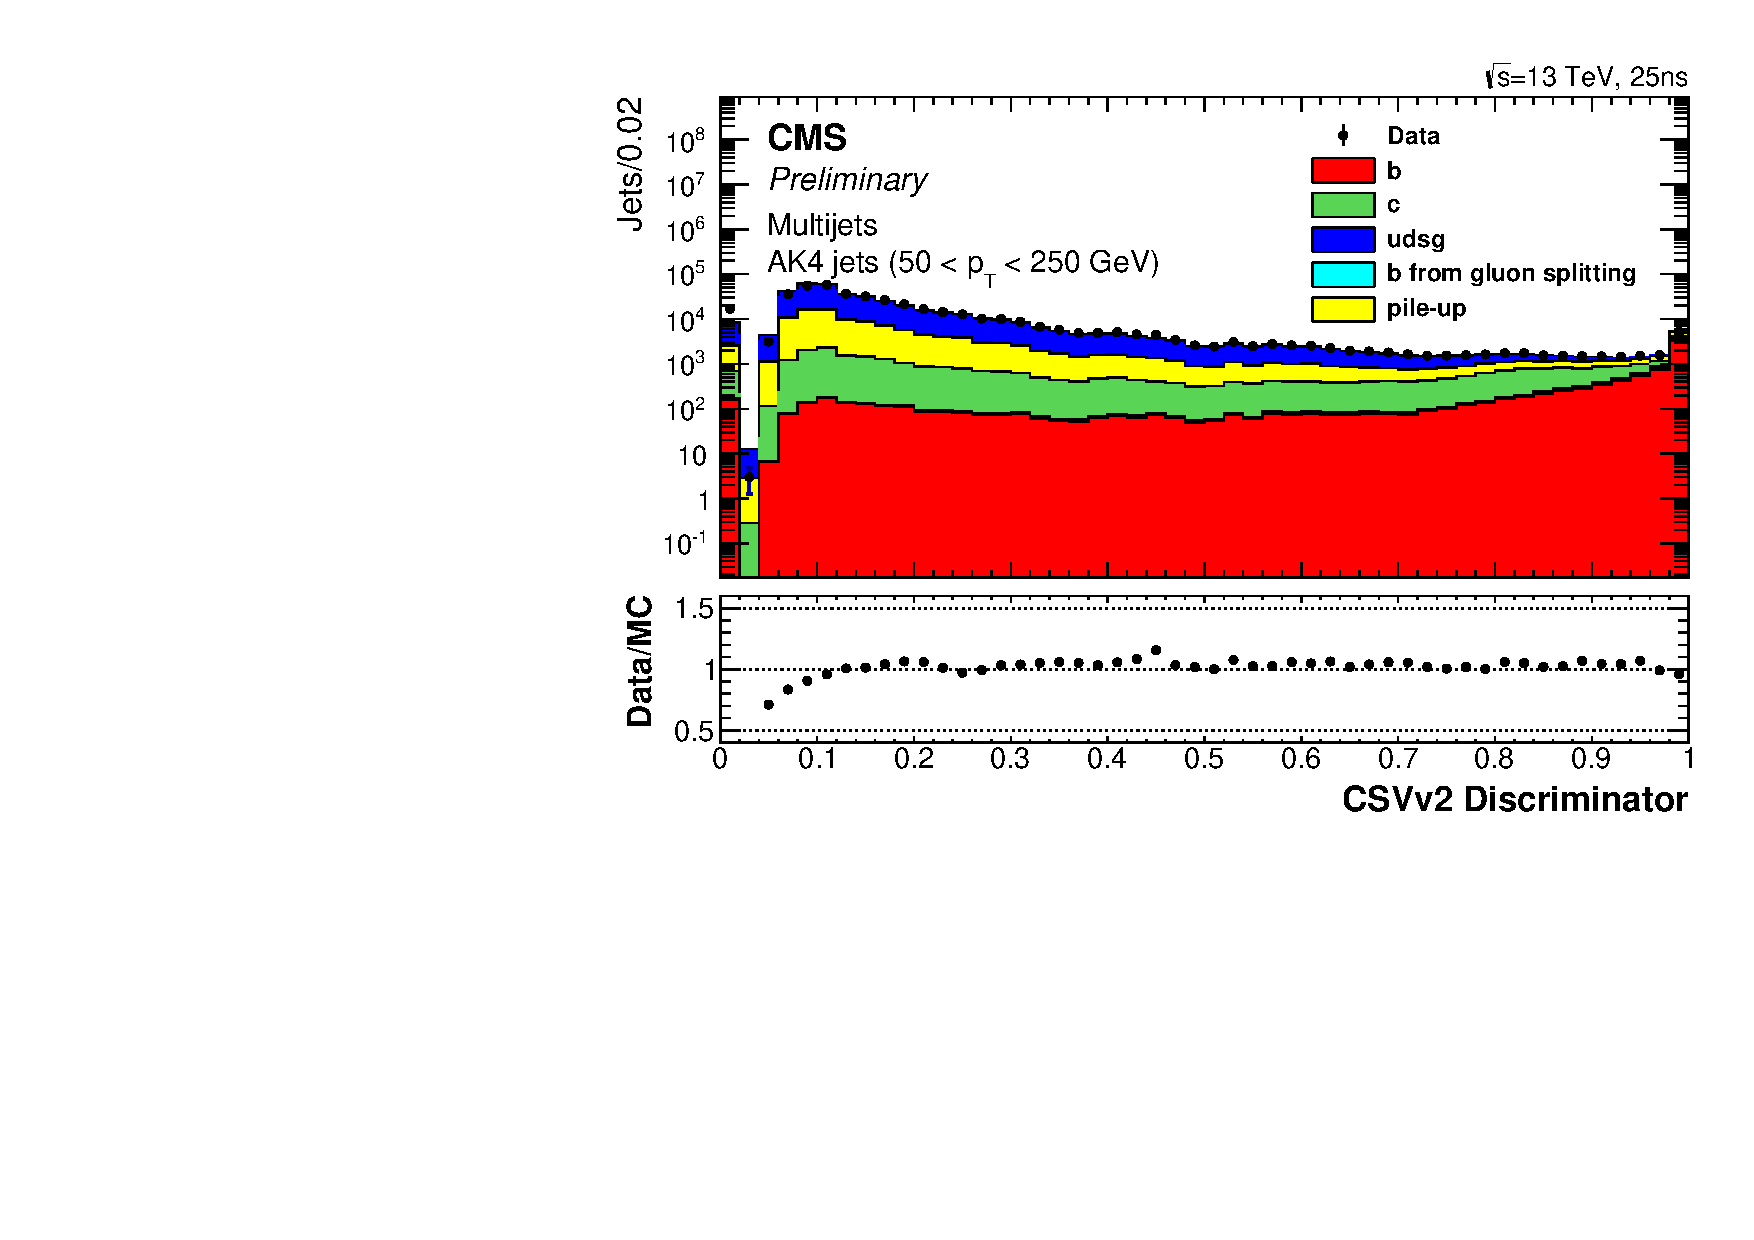
\includegraphics[width=0.5\textwidth]{figs/csvv2_multijet_13TeV.pdf}
\caption{Discriminator values for the CSVv2 algorithm for an inclusive multi-jet topology, where the total number of entries in the simulation is normalized to the observed number of entries in the data.}
\label{fig:CSVv2_multijet}
\end{figure}

%%---------------------- MET definitions ---------------------- %%
\section{Missing transverse energy}
\label{sec:MET}
A crucial aspect of this search requires the precise modeling of the missing transverse energy, and denoted by \ptmiss. Owing to momentum and energy conservation, \ptmiss corresponds to the magnitude of the transverse momentum that is carried by weakly interacting particles, such as neutrinos. This observable is of particular importance in the search for \ttDM, since the neutral DM particles are also predicted to interact weakly, hence they will escape the detector volume without being detected. The measurement of \ptmiss relies heavily on the detectable and reconstructed physics objects mentioned in the preceding sections. Thus, \ptmiss is defined as the imbalance in the transverse momentum of all particles that interact with the detectors. As described in \SectionRef{sec:PF}, the CMS PF algorithm provides a list of PF candidates reconstructed from correlation of subdetector signals. It then follows that the \ptvecmiss is defined as the negative vectorial sum of the transverse momenta of all PF candidates in the event, such that,

\begin{equation}
  \ptvecmiss = -\sum_{i=\mathrm{PF\:particles}}{\vec{p}_{\text{T},i}}
  \label{eq:met}
\end{equation}

The measurement of the \ptmiss can be mismeasured as a cause of a variety of reasons. The nonlinear response of the calorimeter for neutral and charged hadrons due to its noncompensating nature, minimum energy thresholds in the calorimeters, inefficiencies in the tracker, or neutrinos from semileptonic particle decays are a sources from which bias can be introduced in the \ptmiss measurement. In order to mitigate these biases, the \ptmiss derived is corrected for using jet energy scale corrections, so \EquationRef{eq:met} then becomes,

\begin{equation}
  \ptvecmiss = -\sum_{i=\mathrm{PF\:particles}}{\vec{p}_{\text{T},i}} - \sum_{\mathrm{jets}}{\Big(\vec{\pt}^{\mathrm{corr}}_{\mathrm{,jet}} - \vec{\pt}_{\mathrm{,jet}}\Big)}.
  \label{eq:Type1met}
\end{equation} 

The quantity in~\EquationRef{eq:Type1met} is the \MET quantity used throughtout this work and shown in all experimental plots in the following chapters.

\begin{comment}
%%---------------------- Event selection ---------------------- %%
\section{Event Selection}
\label{sec:selection}

The objects defined in \SectionRef{sec:leps}-\ref{sec:MET} are all employed to target the selection of events consistent with \ttMET where both tops have leptonically decaying W bosons. The selection for the signal region is the following,

\begin{itemize}
\item Two ``Tight'' leptons with opposite charge ($ee$ or $e\mu$ or $\mu\mu$) with $\pt>25\:\GeV$ for the leading lepton and $\pt>15\:\GeV$ for the trailing lepton,
\item No additional leptons with $\pt>10\:\GeV$ and passing ``Loose'' muon or ``Veto'' electron criteria,
\item Two or more jets where at least one jet is b-tagged,
\item $M_{\ell\ell}>20\:\GeV$,
\item $|M_{\ell\ell} - M_Z|>15\:\GeV$ for $ee$ and $\mu\mu$ events,
\item $\ptmiss>50\:\GeV$,
\end{itemize}

Dilepton candidate events with an invariant mass $M_{\ell\ell}<20\:\GeV$ are removed in order to suppress any backgrounds from low-mass Drell-Yan processes, as well as any contributions from heavy-flavor resoncances. The requirement for events in the same flavor ($ee$ and $\mu\mu$) channel to have an invariant mass $\pm15\:\GeV$ away from the Z boson pole mass is also used to reject $Z(\ell\ell)$ background events. The moderate requirement of \ptmiss$>50\:\GeV$ aims to further suppress contamination from DY events in the same flavor channel.

\subsection{The \mttll variable}
\label{subsec:mt2ll}
Along with categorization according to lepton flavor (same or opposite), events are also categorized based on the stransverse mass quantity, \mttll, defined as,

\begin{equation}
M_{\text{T2}}^{\ell\ell} = \min_{\vec{p}^{\text{miss}}_{\text{T1}}+\vec{p}^{\text{miss}}_{\text{T2}}=\vec{p}^{\text{miss}}_{\text{T}}}
\left(\max\left[M_{\text{T}}\left(\vec{p}^{\ell_1}_{\text{T}},\vec{p}^{\text{miss}}_{\text{T1}}\right),\:M_{\text{T}}\left(\vec{p}^{\ell_2}_{\text{T}},\vec{p}^{\text{miss}}_{\text{T2}}\right)\right]\right),
\label{eq:mt2ll}
\end{equation}

\mttll is partially motivated from the transverse mass, denoted $M_{\text{T}}\left(\vec{p}^{\ell}_{\text{T}},\vec{p}^{\text{miss}}_{\text{T}}\right)$ in \EquationRef{eq:mt2ll}, where the most notable use of \mt is in the measurement of the $W$ boson mass in the $W\rightarrow\ell\nu$ decay mode. The transverse mass, defined in the context of a leptonic $W$ boson decay, is as follows,

\begin{equation}
  M_{\text{T}} = \sqrt{M_{\ell}^{2} + M_{\nu}^{2} + 2(E_{\text{T}}^{\ell}E_{\text{T}}^{\nu} - \vec{p}_{\text{T}}^{\ell}\cdot\vec{p}_{\text{T}}^{\nu})}
\end{equation}

where $M_{\ell}$ and $M_{\nu}$ are the masses of the lepton and neutrino, respectively, and $\vec{p}\
_{\text{T}}^{\ell}$ and $\vec{p}_{\text{T}}^{\nu}$ are their transverse momenta. $E_{\text{T}}^{\ell}$ and $E_{\text{T}}^{\nu}$ denote their transverse energies. 

The utility of $M_{\text{T}}$ is best for cases wherein one missing particle is expected (i.e. the neutrino in the leptonic $W$ decay). However, once more than one missing particle is expected in an event, it is no longer possible to calculate the \mt since the \pt of an individual missing particle cannot be resolved. Recalling that \ttDM production and decay follows this route:

\begin{equation}
pp \rightarrow t\bar{t} + \phi \rightarrow W^{+} b + W^{-} \bar{b} + \XX \rightarrow \ell^{+} \nu b + \ell^{-} \bar{\nu} \bar{b} + \XX,
\end{equation}

a signal event is expected to contain four particles that leave their signature in the detector collectively as \ptmiss, namely the $\nu,\:\bar{\nu},\:\chi,\:\bar{\chi}$. Similarly, in the case of the SM \ttll process, the two lepton neutrinos are the sole contributors to the total \ptvecmiss, and as postulated by the authors in~\cite{Lester:1999tx}, if the $\vec{\pt}^{\nu}$ and $\vec{\pt}^{\bar{\nu}}$ were obtainable, the maximum \mt value is bounded from above by the $W$ boson mass such that,

\begin{equation}
  M_{W}^{2} \geq \max{\{M_{\text{T}}^{2}\left(\vec{p}^{\ell^{+}}_{\text{T}}, \vec{p}^{\nu}_{\text{T}}\right), M_{\text{T}}^{2}\left(\vec{p}^{\ell^{-}}_{\text{T}}, \vec{p}^{\bar{\nu}}_{\text{T}}\right)\}}.
\end{equation} 

The partitioning of the \ptvecmiss is however unknown, since neither the energy nor direction of either neutrino four-vector can be resolved, so the best that can be assumed is, 

\begin{equation}
  M_{W} \geq M_{\text{T2}}^{\ell\ell} = \min_{\vec{p}^{\text{miss}}_{\text{T1}}+\vec{p}^{\text{miss}}_{\text{T2}}=\vec{p}^{\text{miss}}_{\text{T}}}\left(\max\left\{M_{\text{T}}\left(\vec{p}^{\ell_1}_{\text{T}},\vec{p}^{\text{miss}}_{\text{T1}}\right),\:M_{\text{T}}\left(\vec{p}^{\ell_2}_{\text{T}},\vec{p}^{\text{miss}}_{\text{T2}}\right)\right\}\right).
\label{eq:mt2ll_2}
\end{equation}

The minimization in \EquationRef{eq:mt2ll_2} occurs over all the possible two-way partitions of \ptvecmiss in the event. For the case of the SM \ttll background, a kinematic endpoint in the \mttll distribution, shown in~\FigureRef{fig:mt2ll}, occurs at the $W$ boson pole mass. With this in mind, two signal regions are formed using the \mttll variable, where events with \mttll$>110\:\GeV$ comprise the high signal purity region, since the signal is not expected to be contained in the region below the $M_W$ as is the case for the SM \ttll background. The low signal purity category is formed by the remaining events, for which \mttll$<110\:\GeV$.

\begin{figure}
  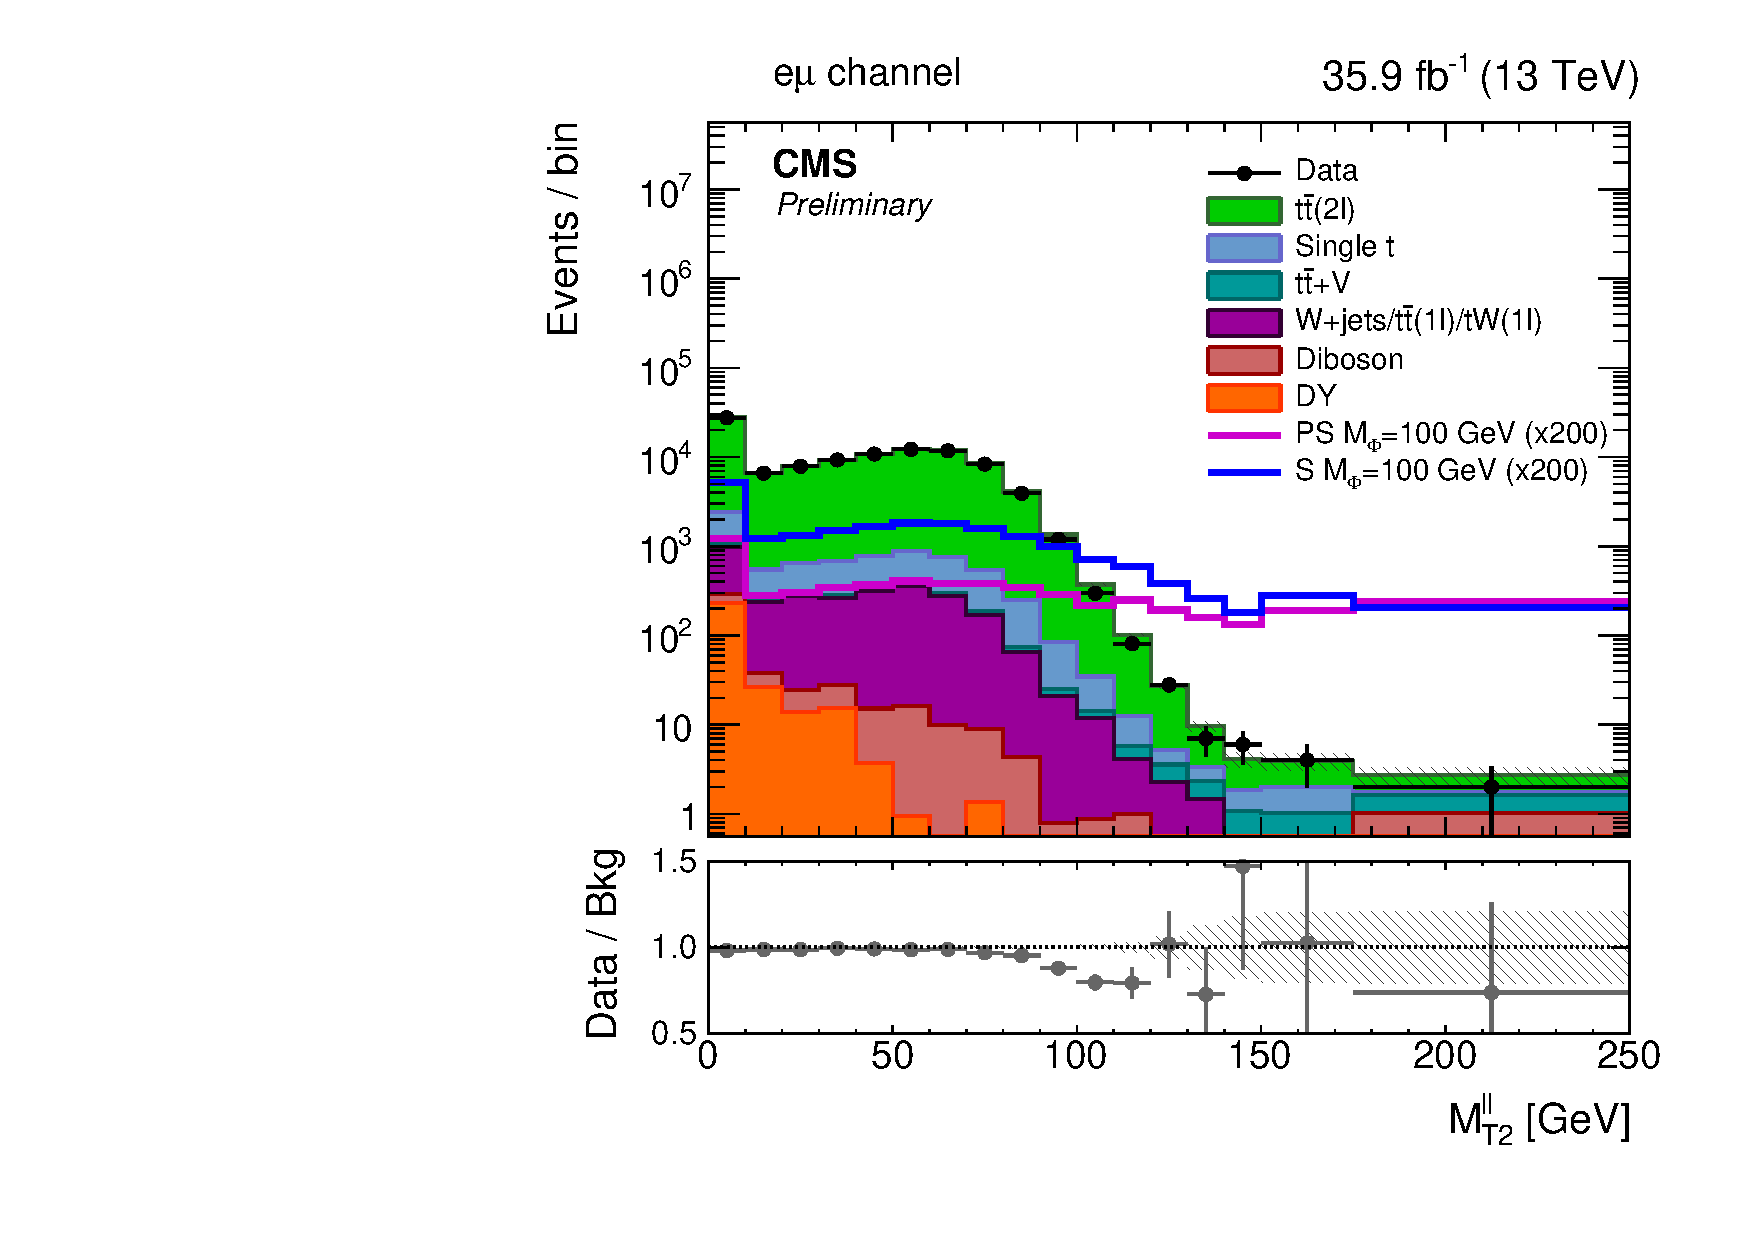
\includegraphics[width=0.6\textwidth]{figs/mt2log_em.pdf}
  \caption{The \mttll distribution in data and simulation for events passing selection requirements for the $e\mu$ channel. The distribution of two example signals (scalar and pseudoscalar mediator, $m_{\phi/a} = 100\:\GeV$) with $m_{\chi}=1\:\GeV$ is scaled up by a factor of 200. The last bin includes overflow. Uncertainties are statistical only.}
  \label{fig:mt2ll}
\end{figure}
\end{comment}


\begin{comment}
Here are some funky floats using ``continued captions'', i.e. for a semantically
collected group of float contents which are too numerous to fit into a single
float, such as the pretty circles in the following figure:

\newcommand{\circleimg}[1]{%
\begin{tikzpicture}
  \draw[color=black,fill=#1,thick] (1,0) circle (1.5cm);
\end{tikzpicture}%
}

\begin{figure}[hb]
  \subfloat[][Example 1a]{\label{fig:cc1a}\circleimg{red!80}}\quad
  \subfloat[][Example 1b]{\label{fig:cc1b}\circleimg{green!70!yellow}}\quad
  \subfloat[][Example 1c]{\label{fig:cc1c}\circleimg{blue!80}}\quad
  \subfloat[][Example 1d]{\label{fig:cc1d}\circleimg{orange!80!yellow}}
  \caption{Demonstration of \texttt{subfig} continued captions.}
  \label{fig:cc1}
\end{figure}

\begin{figure}[p]
  \ContinuedFloat
  \subfloat[][Example 1e]{\label{fig:cc1e}\circleimg{violet}}\quad
  \subfloat[][Example 1f]{\label{fig:cc1f}\circleimg{cyan}}\quad
  \subfloat[][Example 1g]{\label{fig:cc1g}\circleimg{magenta}}\quad
  \subfloat[][Example 1h]{\label{fig:cc1h}\circleimg{yellow}}
  \caption[]{Demonstration of \texttt{subfig} continued captions (continued).}
\end{figure}

\noindent
This mechanism means that the same float label is used for both pages of
floats. Note that we can refer to \FigureRef{fig:cc1} in general, or to
\FigureRef{fig:cc1g} on \PageRef{fig:cc1g} in particular!

\noindent
Just for the hell of it, let's also refer to \SectionRef{sec:neutralmixing}.
\end{comment}

  \chapter{Signal simulation and event selection} 
\label{chap:signalsel}

\section{\ttDM simplified models}
\label{sec:simpmodels}

The dark matter collider signal under investigation is characterized by the production of a top quark pair recoiling against a spin-0 mediator which decays to a pair of dark matter particles, as shown in~\FigureRef{fig:ttDM}. As described in greater detail in Sec, this model predicts the production of dark matter via a scalar (\phi) or pseudoscalar ($a$) mediator, which couples to SM fermions (in this case top quarks) and the Dirac fermion DM particles, with unitary coupling strength (\gq=\gDM=1). 

The most important characteristic of \ttDM models is the \pt of the $\chi\bar{\chi}$ system. This quantity is equivalent to the mediator \pt and is translated to the \ptmiss detector observable in an event. The \ptmiss spectra for the \ttDM models, although dependent on the mediator mass, are expected to peak at higher values than that of the SM \ttbar process, owing to the additional contribution from the $\chi\bar{\chi}$ system. In general, the mediator \pt spectrum broadens with increasing mediator mass, as demonstrated in~\FigureRef{fig:SvPSmedpt}, where the \pt is shown for various scalar and pseudoscalar mediator masses with $M_\chi=1\:\GeV$. It is also the case that at low masses, the pseudoscalar \pt is harder than the scalar \pt of equivalent mediator mass, however the distributions converge to at higher mediator mass. The trend of broadening mediator \pt spectra with increasing mediator mass does not hold in the off-shell regime where the mediator mass is less than twice the DM fermion mass ($2M_\chi > M_\phi$). In the off-shell regime, the \pt of the mediator is not dependent on the mass, and in addition, if the $M_\chi$ is varied for a fixed mediator mass, the \pt distribution is harder for the off-shell production rather than the on-shell. Due to the finite mediator width, in the area near the on/off-shell threshold, the kinematics will contain contributions from both types of production, as seen in~\FigureRef{fig:dmf_medpt2}. 

\begin{figure}
  \begin{center}
    \feynmandiagram[horizontal=c to h]{
      a [particle=\(\bar{t}\)] -- [fermion] b -- [fermion] c -- [fermion] d -- [fermion] e [particle=\(t\)],
      f [particle=\(g\)] -- [gluon] b,
      g [particle=\(g\)] -- [gluon] d,
      c -- [scalar, edge label=\(\phi \slash a\)] h,
      i [particle=\(\bar{\chi}\)] -- [fermion] h -- [fermion] j [particle=\(\chi\)],
      e -- [opacity=0.0001] i,
      a -- [opacity=0.0001] j,
      i -- [opacity=0.0001] j,
%%      f -- [opacity=0.0001] g,
    };
    \caption{The representative diagram of a top quark pair produced in association with a pair of DM particles ($\chi\bar{\chi}$) which decay via an explicit scalar or pseudoscalar mediator coupled to the tops.}
    \label{fig:ttDM}
  \end{center}
\end{figure}

\begin{figure}[htbp!]
  \begin{center}
    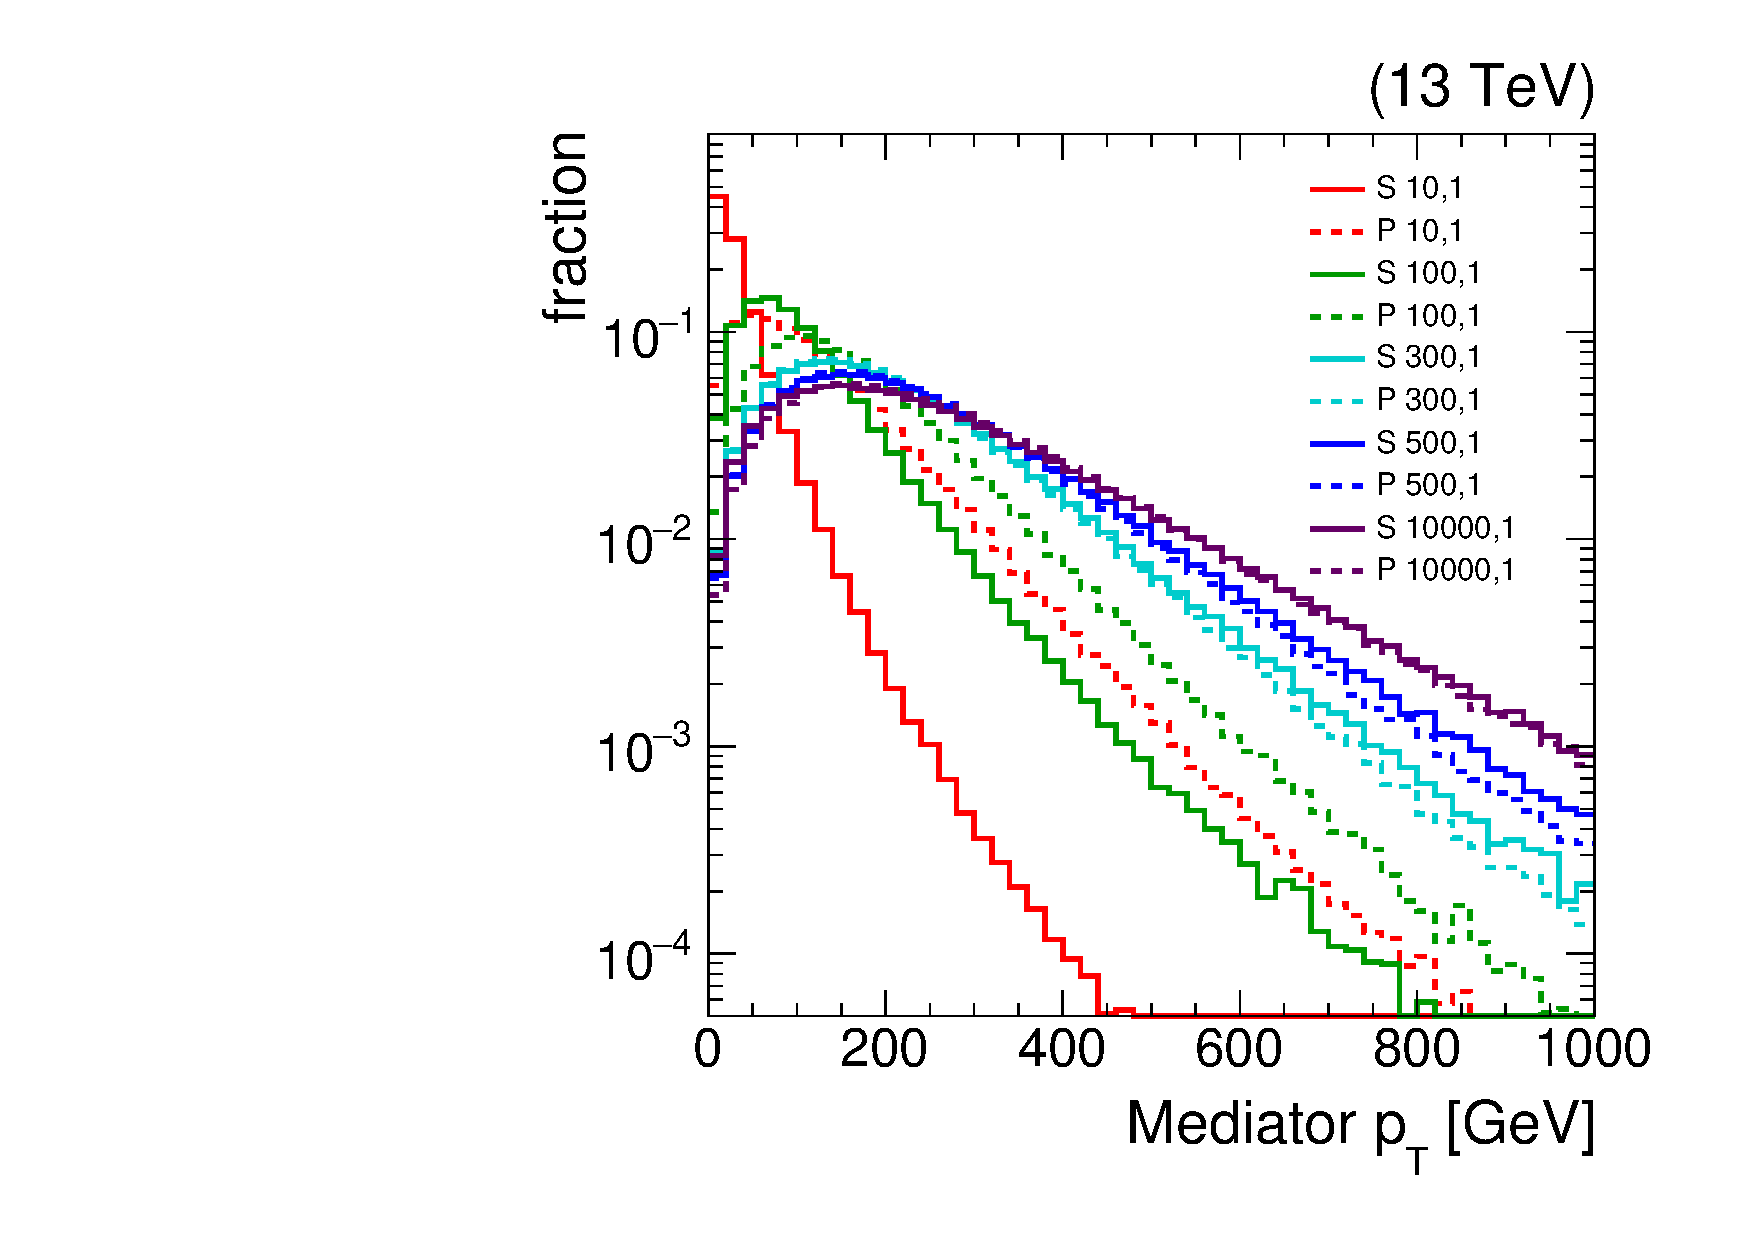
\includegraphics[width=0.48\textwidth]{figs/medptlog.pdf}
    \caption{Generator level \pt distributions for scalar (solid lines) and pseudoscalar (dashed lines) mediators, with $M_\chi=1\:\GeV$, where distributions with the same color have the same mediator mass.}
    \label{fig:SvPSmedpt}
  \end{center}
\end{figure}

\begin{figure}[htbp!]
\begin{center}
  \subfloat[][]{\label{subfig:dmf_off}   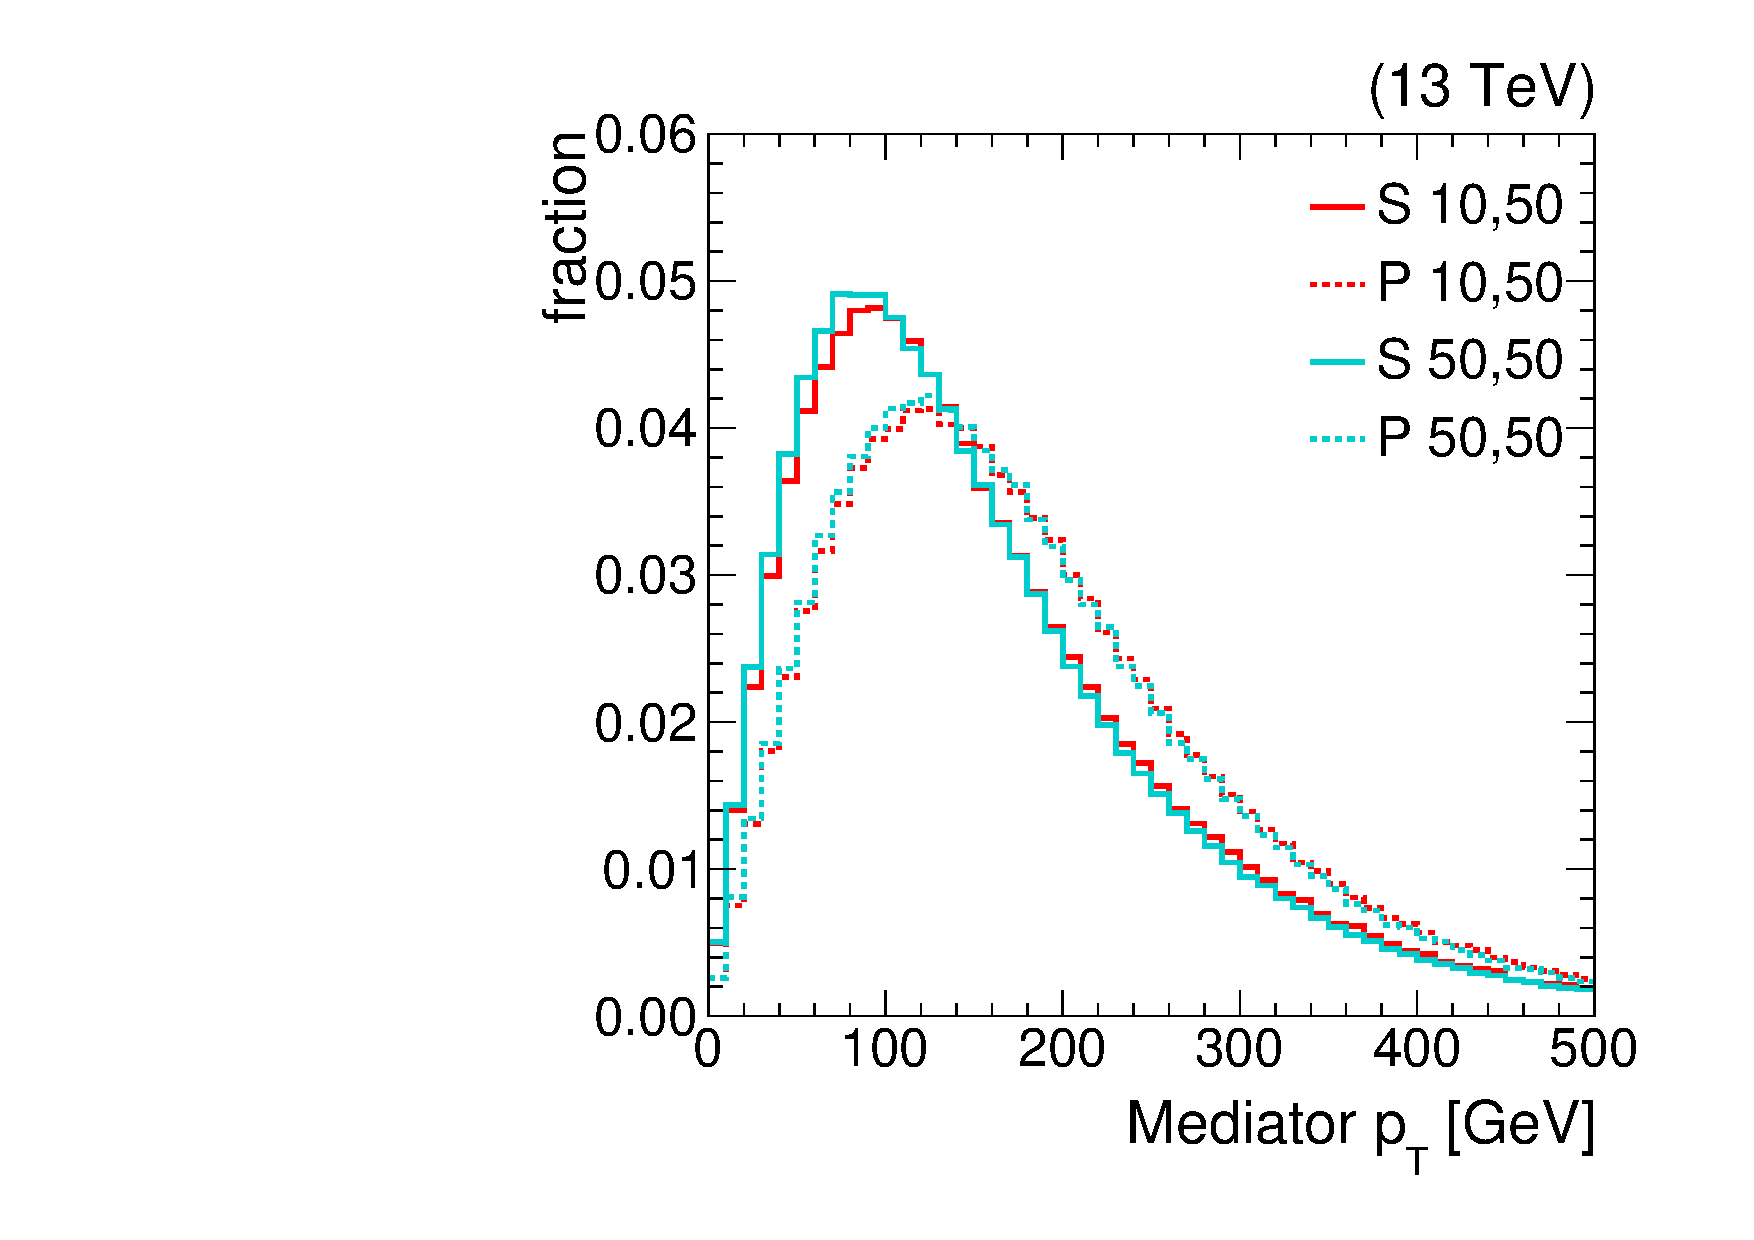
\includegraphics[width=0.48\textwidth]{figs/offshell_medpt.pdf}}
  \subfloat[][]{\label{subfig:dmf_on_off}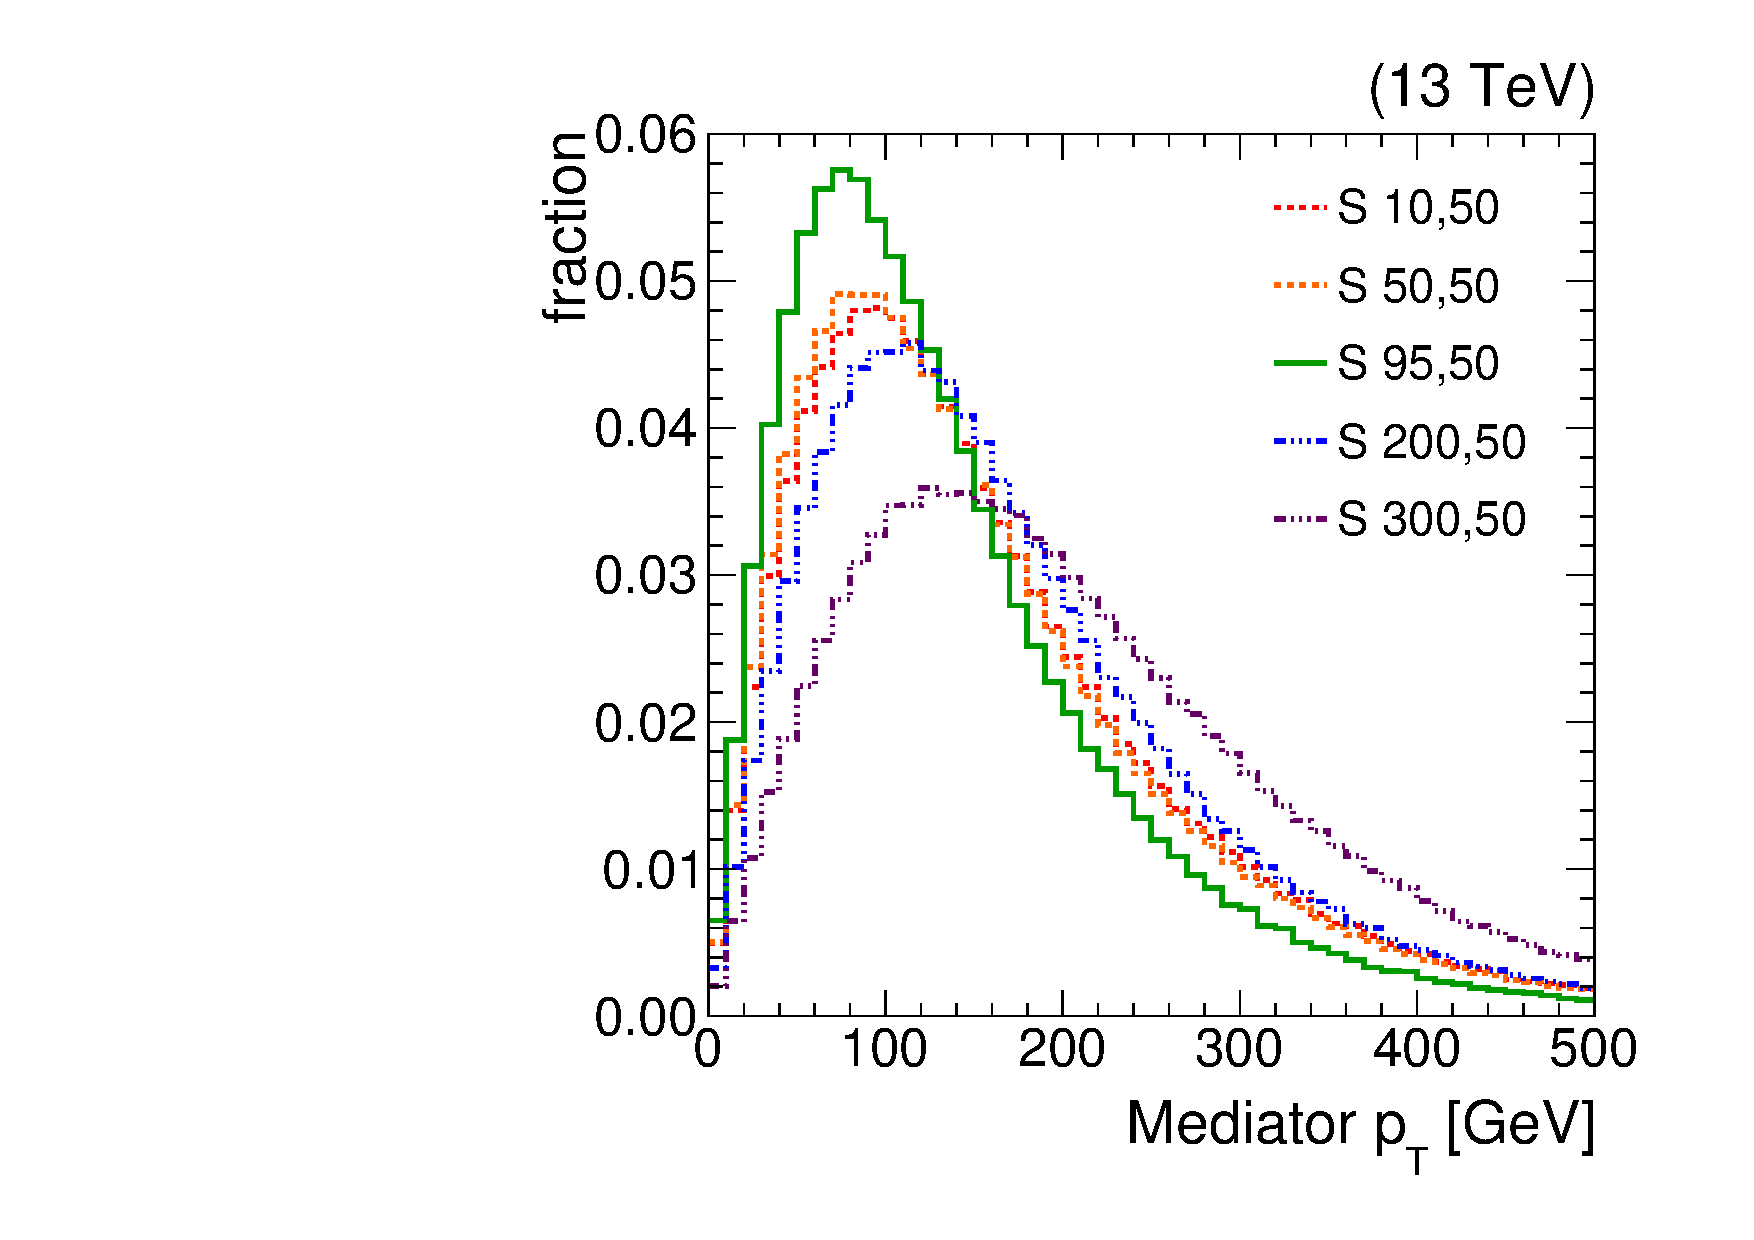
\includegraphics[width=0.48\textwidth]{figs/onshell_vs_offshell_medpt.pdf}}
  \caption{~\protect\subref{subfig:dmf_off} Generator level $\pt$ distributions for off-shell production, with solid lines for scalar and dashed lines for pseudoscalar, and $M_\chi=50\:\GeV$.\protect\subref{subfig:dmf_on_off} Near the on-shell/off-shell threshold (green solid line), the kinematics has contributions from on-shell and off-shell production.}
  \label{fig:dmf_medpt2}
\end{center}
\end{figure}

The \ttDM signals are generated in the dilepton final state at LO accuracy in perturbative QCD using \AMCATNLO \textsc{v2.2.2}~\cite{Alwall:2014hca} with up to one additional jet. The MLM parton-jet matching prescription~\cite{Mangano:2006rw} is used to match jets from the matrix element to the parton shower. The spin correlations in the decays of top quarks are preserved through the use of \MadSpin. The partial width formulae given in ~\cite{PhysRevD.91.055009} are used to calculate the minimum decay widths for the mediators. The calculation assumes that the mediator couples only to SM quarks and the fermion DM particle (\chi), and decays exclusively to a DM pair.  

%%---------------------- Event selection ---------------------- %%
\section{Signal region event selection}
\label{sec:selection}

The objects defined in Sec.~\ref{sec:leps}-\ref{sec:MET} are all employed to target the selection of events consistent with \ttMET where both tops have leptonically decaying W bosons. The selection is as follows,

\begin{itemize}
\item Two ``Tight'' leptons with opposite charge ($ee$ or $e\mu$ or $\mu\mu$) with $\pt>25\:\GeV$ for 
the leading lepton and $\pt>15\:\GeV$ for the trailing lepton,
\item No additional leptons with $\pt>10\:\GeV$ and passing ``Loose'' muon or ``Veto'' electron criter
ia,
\item Two or more jets where at least one jet is b-tagged,
\item $M_{\ell\ell}>20\:\GeV$,
\item $|M_{\ell\ell} - M_Z|>15\:\GeV$ for $ee$ and $\mu\mu$ events,
\item $\ptmiss>50\:\GeV$,
\end{itemize}

Dilepton candidate events with an invariant mass $M_{\ell\ell}<20\:\GeV$ are removed in order to suppress any backgrounds from low-mass Drell-Yan processes, as well as any contributions from heavy-flavor resonances. The requirement for events in the same flavor ($ee$ and $\mu\mu$) channel to have an invariant mass $\pm15\:\GeV$ away from the Z boson pole mass is also used to reject $Z(\ell\ell)$ background events. The moderate requirement of \ptmiss$>50\:\GeV$ aims to further suppress contamination from DY events in the same flavor channel.

\subsection{The \mttll variable}
\label{subsec:mt2ll}

Along with categorization according to lepton flavor (same or opposite), events are also categorized based on the stransverse mass quantity, \mttll, defined as,

\begin{equation}
  M_{\text{T2}}^{\ell\ell} = \min_{\vec{p}^{\text{miss}}_{\text{T1}}+\vec{p}^{\text{miss}}_{\text{T2}}=\vec{p}^{\text{miss}}_{\text{T}}}\left(\max\left[M_{\text{T}}\left(\vec{p}^{\ell_1}_{\text{T}},\vec{p}^{\text{miss}}_{\text{T1}}\right),\:M_{\text{T}}\left(\vec{p}^{\ell_2}_{\text{T}},\vec{p}^{\text{miss}}_{\text{T2}}\right)\right]\right),
  \label{eq:mt2ll}
\end{equation}

\mttll is partially motivated from the transverse mass, denoted $M_{\text{T}}\left(\vec{p}^{\ell}_{\text{T}},\vec{p}^{\text{miss}}_{\text{T}}\right)$ in Eq.~\ref{eq:mt2ll}, where the most notable use of \mt is in the measurement of the $W$ boson mass in the $W\rightarrow\ell\nu$ decay mode. The transverse mass, defined in the context of a leptonic $W$ boson decay, is as follows,

\begin{equation}
  M_{\text{T}} = \sqrt{M_{\ell}^{2} + M_{\nu}^{2} + 2(E_{\text{T}}^{\ell}E_{\text{T}}^{\nu} - \vec{p}_{\text{T}}^{\ell}\cdot\vec{p}_{\text{T}}^{\nu})}
\end{equation}

where $M_{\ell}$ and $M_{\nu}$ are the masses of the lepton and neutrino, respectively, and $\vec{p}\
_{\text{T}}^{\ell}$ and $\vec{p}_{\text{T}}^{\nu}$ are their transverse momenta. $E_{\text{T}}^{\ell}$ and $E_{\text{T}}^{\nu}$ denote their transverse energies. 

The utility of $M_{\text{T}}$ is best for cases wherein one missing particle is expected (i.e. the neutrino in the leptonic $W$ decay). However, once more than one missing particle is expected in an event, it is no longer possible to calculate the \mt since the \pt of an individual missing particle cannot be resolved. Recalling that \ttDM production and decay follows this route:

\begin{equation}
pp \rightarrow t\bar{t} + \phi \rightarrow W^{+} b + W^{-} \bar{b} + \XX \rightarrow \ell^{+} \nu b + \ell^{-} \bar{\nu} \bar{b} + \XX,
\end{equation}

a signal event is expected to contain four particles that leave their signature in the detector collectively as \ptmiss, namely the $\nu,\:\bar{\nu},\:\chi,\:\bar{\chi}$. Similarly, in the case of the SM \ttll process, the two lepton neutrinos are the sole contributors to the total \ptvecmiss, and as postulated by the authors in~\cite{Lester:1999tx}, if the $\vec{\pt}^{\nu}$ and $\vec{\pt}^{\bar{\nu}}$ were obtainable, the maximum \mt value is bounded from above by the $W$ boson mass such that,

\begin{equation}
  M_{W}^{2} \geq \max{\{M_{\text{T}}^{2}\left(\vec{p}^{\ell^{+}}_{\text{T}}, \vec{p}^{\nu}_{\text{T}}\right), M_{\text{T}}^{2}\left(\vec{p}^{\ell^{-}}_{\text{T}}, \vec{p}^{\bar{\nu}}_{\text{T}}\right)\}}.
\end{equation} 

The partitioning of the \ptvecmiss is however unknown, since neither the energy nor direction of either neutrino four-vector can be resolved, so the best that can be assumed is, 

\begin{equation}
  M_{W} \geq M_{\text{T2}}^{\ell\ell} = \min_{\vec{p}^{\text{miss}}_{\text{T1}}+\vec{p}^{\text{miss}}_{\text{T2}}=\vec{p}^{\text{miss}}_{\text{T}}}\left(\max\left\{M_{\text{T}}\left(\vec{p}^{\ell_1}_{\text{T}},\vec{p}^{\text{miss}}_{\text{T1}}\right),\:M_{\text{T}}\left(\vec{p}^{\ell_2}_{\text{T}},\vec{p}^{\text{miss}}_{\text{T2}}\right)\right\}\right).
\label{eq:mt2ll_2}
\end{equation}

The minimization in Eq.~\ref{eq:mt2ll_2} occurs over all the possible two-way partitions of \ptvecmiss in the event. For the case of the SM \ttll background, a kinematic endpoint in the \mttll distribution, shown in~\FigureRef{fig:mt2ll}, occurs at the $W$ boson pole mass. With this in mind, two signal regions are formed using the \mttll variable, where events with \mttll$>110\:\GeV$ comprise the high signal purity region, since the signal is not expected to be contained in the region below the $M_W$ as is the case for the SM \ttll background. The low signal purity category is formed by the remaining events, for which \mttll$<110\:\GeV$.

\begin{figure}
  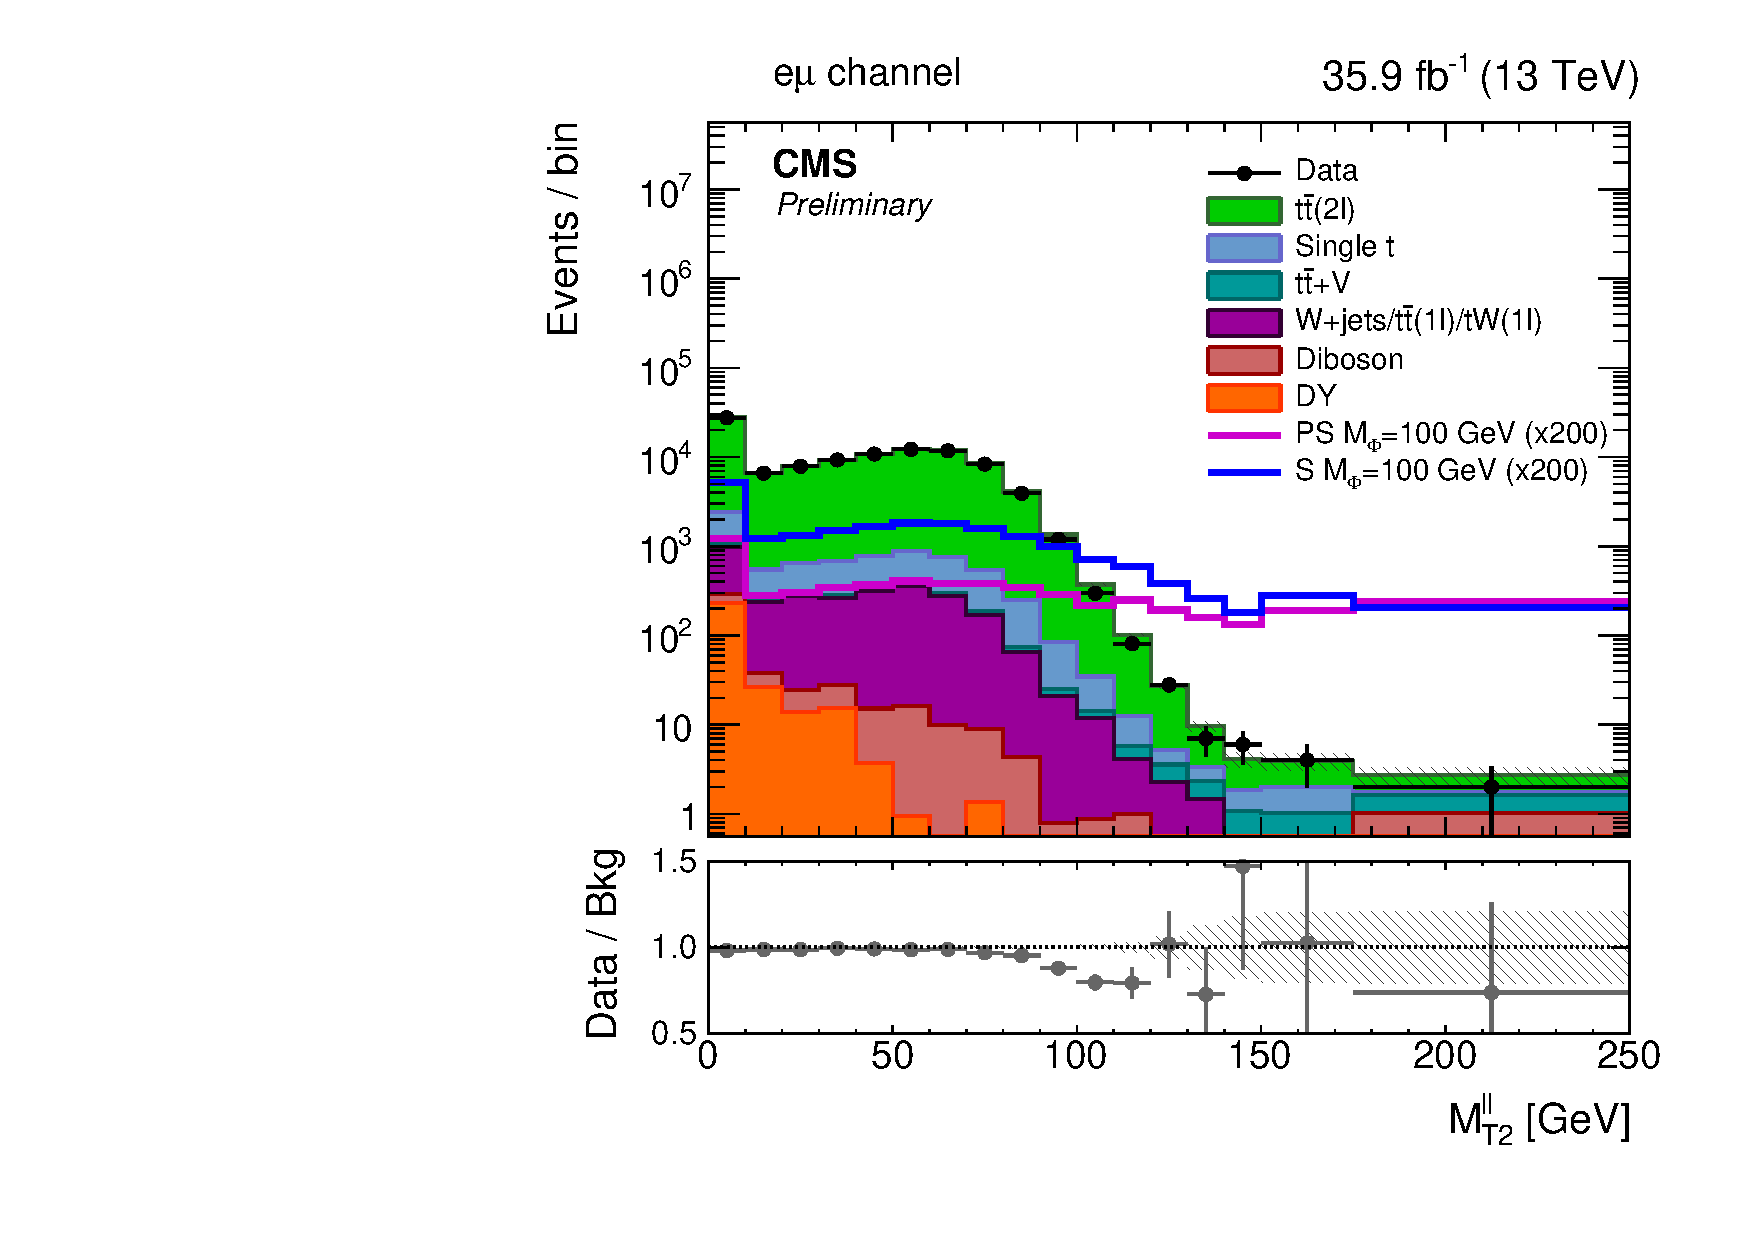
\includegraphics[width=0.6\textwidth]{figs/mt2log_em.pdf}
  \caption{The \mttll distribution in data and simulation for events passing selection requirements for the $e\mu$ channel. The distribution of two example signals (scalar and pseudoscalar mediator, $M_{\phi/a} = 100\:\GeV$) with $M_{\chi}=1\:\GeV$ is scaled up by a factor of 200. The last bin includes overflow. Uncertainties are statistical only.}
  \label{fig:mt2ll}
\end{figure}

  \chapter{Background processes}
\label{chap:backgrounds}

Two classes of background processes are present in this search: reducible and irreducible. For the former category, a particle in the background process may ``fake'' the signature of a particle that is expected in the signal process. On the contrary, in the case of the latter category, the final state topology of the background process yields the same expected particles as a potential signal process. A key feature of reducible backgrounds is the ability to suppress such processes by employing the selection cuts as described in Sec.~\ref{sec:selection}. Furthermore, some of the reducible background contributions are estimated using data-driven techniques. In large part, however, the dominant backgrounds in the search are estimated from simulations.

Sec.~\ref{sec:tt2l}-\ref{sec:fakes} describe the relevant SM backgrounds in the search for \ttllDM. The production cross sections at $\sqrt{s}=13\:\TeV$ for these backgrounds are shown in~\FigureRef{fig:SMxsec}, giving a sense of the relative importance of the processes. The phase space targeted by the selection requirements as described in Sec.~\ref{sec:selection} also affects the relative hierarchy of the backgrounds, though it remains true that processes with larger cross sections, such as \ttbar and Drell-Yan, are dominant in the regions of highest sensitivity.

\begin{figure}
  \begin{center}
    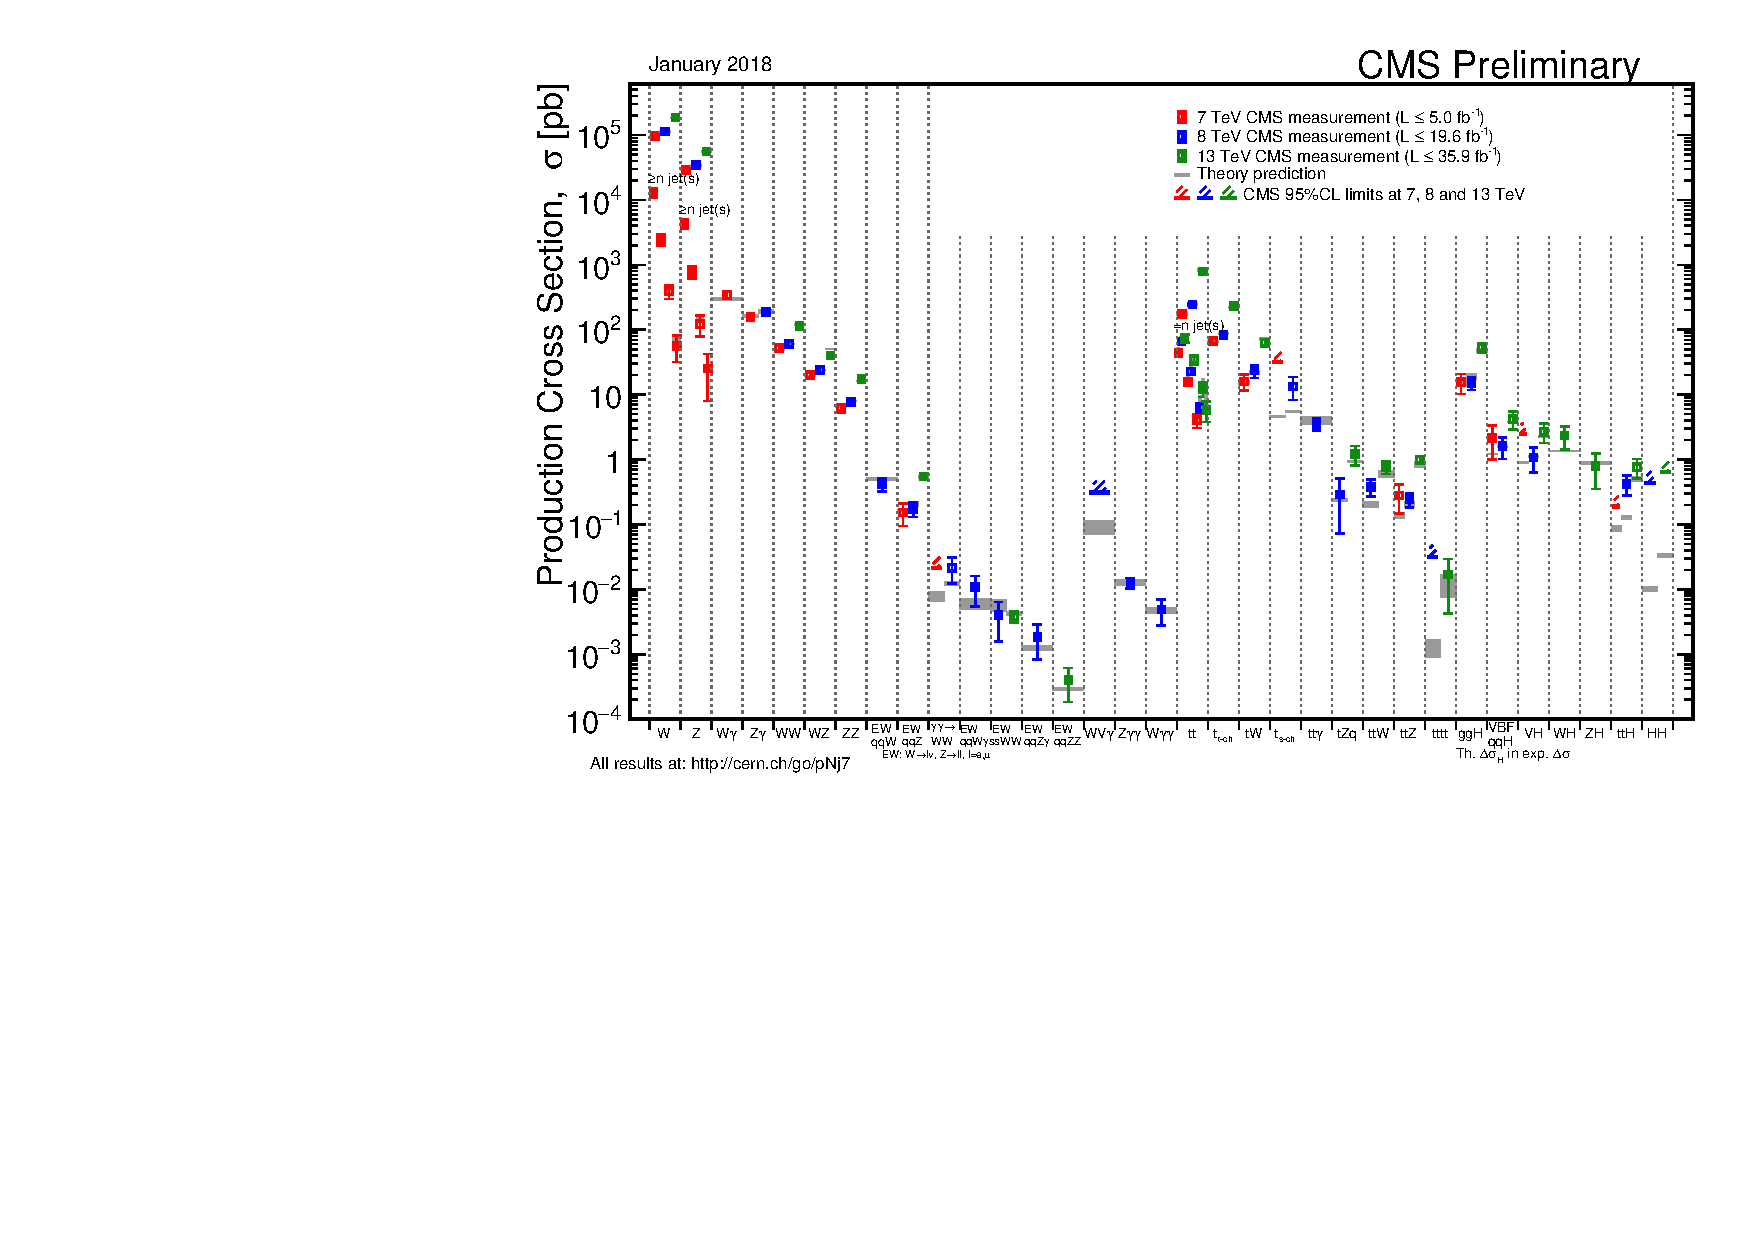
\includegraphics[width=\textwidth]{figs/SigmaNew_v0.pdf}
    \caption{Summary of the cross section measurements of SM processes as of January 2018 with data collected by the CMS experiment at $\sqrt{s}=7,\:8,\:\text{and}\: 13\:\TeV$. }
    \label{fig:SMxsec}
  \end{center}
\end{figure}

\begin{figure}
  \begin{center}
    \subfloat[][]{\label{fig:gg_tt}
      \feynmandiagram[horizontal=b to c]{
        a [particle=\(g\)] -- [gluon] b -- [gluon] c,
        d [particle=\(g\)] -- [gluon] b,
        e [particle=\(\bar{t}\)] -- [fermion] c,
        c -- [fermion] f [particle=\(t\)],
      };
    }
    \hspace{0.5cm}
    \subfloat[][]{\label{fig:gg_tt2}
      \feynmandiagram[vertical=b to d]{
        a [particle=\(g\)] -- [gluon] b,
        c [particle=\(\bar{t}\)] -- [fermion] b -- [fermion] d -- [fermion] f [particle=\(t\)], 
        e [particle=\(g\)] -- [gluon] d,
        a -- [opacity=0.0001] e,
        c -- [opacity=0.0001] f,
      };
    }
    \hspace{0.5cm}
    \subfloat[][]{\label{fig:qq_tt}
      \feynmandiagram[horizontal=b to d]{
        a [particle=\(q\)] -- [fermion] b -- [fermion] c [particle=\(\bar{q}\)],
        b -- [gluon] d,
        f [particle=\(\bar{t}\)] -- [fermion] d -- [fermion] e [particle=\(t\)],
      };
    }
  \end{center}
  \caption{Leading order \ttbar production diagrams probed at the LHC via~\protect\subref{fig:gg_tt},~\protect\subref{fig:gg_tt2} gluon fusion, and~\protect\subref{fig:qq_tt} quark-antiquark annihilation.}
\label{fig:tt2l_feyn}
\end{figure}
%%------------------------- tt2l -------------------------%%  
\section{\ttll}
\label{sec:tt2l}
SM \ttll is the dominant background contribution and is irreducible, owing to the similarity of the final state topology with the signal processes topology. At the LHC, approximately 90\% of \ttbar events are produced via gluon fusion as shown in~\FigureRef{fig:gg_tt} and ~\FigureRef{fig:gg_tt2}, in contrast to the Tevatron at Fermilab, where quark-antiquark annihilation shown in~\FigureRef{fig:qq_tt} constituted roughly 85-90\% of the relative \ttbar production. 

The theoretical uncertainties incurred at leading order (LO) in perturbative QCD are quite large for \ttbar production. In addition to the LO simulation, the \ttbar process decaying to the dilepton final state is simulated at next-to-leading order (NLO) using the \POWHEG \textsc{v2}~\cite{powheg,powheg2} generator, with the top quark mass assumed to be \mtop=172.5\:\GeV. These events are then interfaced to \Pythia \textsc{v8.2}~\cite{Sjostrand:2014zea} for parton fragmentation, hadronization, and to simulate the underlying event. As pertains to all simulated samples subsequently described, once the \ttll events are showered, the detector response is simulated using the \Geant 4 program~\cite{AGOSTINELLI2003250}. Finally, the \ttll events are normalized to the theoretical cross section calculated at next-to-next-to-leading order (NNLO) in perturbative QCD, which also includes soft-gluon resummation calculations at next-to-next-to-leading-order (NNLL)~\cite{ttxsec1,ttxsec2,ttxsec3,ttxsec4,ttxsec5}. The cross-section folds in the branching fraction of \ttbar to the dilepton final state, which is 10.5\%. The cross-section value used is $\sigma_{\ttll}=87.31\:\mathrm{pb}$.

As mentioned in Sec.~\ref{subsec:mt2ll}, the \ttll background should be suppressed below the kinematic endpoint, $M_W$, in the \mttll distribution. This would only be possible in ideal measurement conditions, however as a cause of detector and energy resolution effects, the mismeasurement of the objects in \ttll background events can contribute to values of \mttll$>\:M_W$. 

%%------------------------- ttV,VV,ST -------------------------%%  
\section{\ttV, diboson, and single top processes}
\label{sec:ttVetc}
Among the more rare processes considered as backgrounds to this search are processes wherein a top quark pair is produced in association with a boson, denoted as \ttV (where V=\gamma, Z, W). In particular for the $\mathrm{t\bar{t}}$+Z process, as shown in~\FigureRef{fig:ttV}, the same final state is expected as the signal so this process falls under the class of irreducible backgrounds. Although the production cross-sections for \ttV processes are orders of magnitude smaller than the \ttbar production cross-section, this background is significant in the high \mttll categories. The moderate \ptmiss requirement is inefficient in \ttV background reduction, since large values of \ptmiss are expected. In addition, the $\mathrm{t\bar{t}}$+Z process will leak into the high \mttll category as a cause of the additional expected \ptmiss from the neutrinos, which bias the minimization over all the two-way partitions of the \ptmiss, resulting in high values of \mttll.

The diboson background processes encompass WW, ZZ, and WZ production where all possible final states (i.e. decays to $q\bar{q}$, $\ell\nu$, $\ell\ell$, and $\nu_\ell\bar{\nu}_\ell$) are considered for the relevant boson. Owing in part to the largest relative production cross-section, the WW process is the dominant diboson process. In particular, the dilepton signal region requirement targets the final state where both W bosons decay to lepton-neutrino pairs. 
 
The single top background is also expected to contribute sub-dominantly in the signal region. The lepton multiplicity requirement serves to suppress the contributions from s- and t-channel production (i.e. processes whose amplitudes go as $\mathscr{M}\sim 1/s$ and $\mathscr{M}\sim 1/t$, where $s$ and $t$ correspond to the Mandelstam variables), as seen in~\FigureRef{fig:s-channel} and~\FigureRef{fig:t-channel}, since only one prompt lepton is expected. Thus, the dilepton final state tW associated production diagram, shown in~\FigureRef{fig:tW}, contributes the most significantly to the single top background.  

Similarly to the \ttll process, the \ttV, diboson, and single top processes are simulated at NLO. The \ttV processes are generated using \AMCATNLO \textsc{v2.2.2}. For single top, the s- and t-channel processes are simulated using \POWHEG \textsc{v2} and interfaced with \MadSpin which decays the top and preserves the spin correlation and any finite width effects in narrow resonance decays. The tW channel, on the other hand, is generated using \POWHEG \textsc{v1} at NLO accuracy and normalized to the approximate NNLO cross-section. The diboson samples are generated at NLO using either \AMCATNLO \textsc{v2.2.2} or \POWHEG \textsc{v2}.
 
\begin{figure}
  \begin{center}
    \subfloat[][\ttV]{\label{fig:ttV}
      \feynmandiagram[vertical=c to b] {
        a [particle=\(q\)] -- [fermion] b -- [fermion] c -- [fermion] d [particle=\(\bar{q}\)],
        b -- [boson, edge label=\(Z\)] e,
        i [particle=\(\bar{\nu}_\ell\)] -- [fermion] e -- [fermion] j [particle=\(\nu_\ell\)],
        c -- [gluon, edge label'=\(g\)] f,
        g [particle=\(\bar{t}\)] -- [fermion] f -- [fermion] h [particle=\(t\)],
%        f -- [opacity=0.0001] e,
%        a -- [opacity=0.0001] d,
      };
    }
    \hspace{1cm}
    \subfloat[][Diboson]{\label{fig:VV}
      \feynmandiagram[vertical=b to c] {
        a [particle=\(q\)] -- [fermion] b -- [fermion] c -- [fermion] d [particle=\(\bar{q}\)],
        b -- [boson] f [particle=\(V\)],
        c -- [boson] e [particle=\(V\)],
        a -- [opacity=0.0001] d,
%        f -- [opacity=0.0001] e,
      };
    }
    \caption{Examples of the~\protect\subref{fig:ttV} \ttV process, and ~\protect\subref{fig:VV} diboson production at LO.}
    \label{fig:diboson_feyn}
  \end{center}
\end{figure}

\begin{figure}
  \begin{center}
    \subfloat[][s-channel]{\label{fig:s-channel}
      \feynmandiagram[horizontal=b to e]{
        a [particle=\(u\)] -- [fermion] b -- [fermion] c [particle=\(d\)],
        d [particle=\(b\)] -- [fermion] e -- [fermion] f [particle=\(t\)],
        b -- [boson, edge label' = \(W^+\)] e,
      };
    }
    \hspace{0.5cm}
    \subfloat[][t-channel]{\label{fig:t-channel}
      \feynmandiagram[vertical=b to e]{
        a [particle=\(u\)] -- [fermion] b -- [fermion] c [particle=\(d\)],
        d [particle=\(b\)] -- [fermion] e -- [fermion] f [particle=\(t\)],
        b -- [boson, edge label = \(W^+\)] e,    
      };
    }
    \hspace{0.5cm}
    \subfloat[][tW-associated]{\label{fig:tW}
      \feynmandiagram[horizontal=b to c]{
        a [particle=\(b\)] -- [fermion] b -- [fermion, edge label=\(b\)] c -- [fermion] d [particle=\(t\)],
        e [particle=\(g\)] -- [gluon] b,
        c -- [boson] f [particle=\(W^-\)], 
      };
    }
    \caption{Single top quark production via~\protect\subref{fig:s-channel} s-channel,~\protect\subref{fig:t-channel} t-channel, and~\protect\subref{fig:tW} in association with a W boson.}
    \label{fig:st_feyn}
  \end{center}
\end{figure}

%%------------------------- DY -------------------------%%  
\section{Drell-Yan}
\label{sec:DY}
\begin{figure}
  \begin{center}
    \subfloat[][]{\label{fig:dy1}
      \feynmandiagram[horizontal=b to d]{
        a [particle=\(q\)] -- [fermion] b -- [fermion] c [particle=\(\bar{q}\)],
        f [particle=\(\ell^{+}\)] -- [fermion] d -- [fermion] e [particle=\(\ell^{-}\)], 
        b -- [boson, edge label=\(\gamma^{*}/Z\)] d,
      };
    } 
    \subfloat[][]{\label{fig:dy2}
      \feynmandiagram[horizontal=b to c] {
        a [particle=\(q\)] -- [fermion] b -- [fermion] c -- [fermion] d [particle=\(q\)],
        e [particle=\(g\)] -- [gluon] b,
        c -- [boson, edge label=\(\gamma^{*}/Z\)] g,
        h [particle=\(\ell^{+}\)] -- [fermion] g -- [fermion] f [particle=\(\ell^{-}\)], 
        d -- [opacity=0.0001] f,
      };
    }  
    \subfloat[][]{\label{fig:dy3}
      \feynmandiagram[vertical=b to c] {
        a [particle=\(q\)] -- [fermion] b -- [fermion] c -- [fermion] d [particle=\(q\)],
        e [particle=\(g\)] -- [gluon] c,
        b -- [boson, edge label=\(\gamma^{*}/Z\)] g,
        h [particle=\(\ell^{+}\)] -- [fermion] g -- [fermion] f [particle=\(\ell^{-}\)], 
        d -- [opacity=0.0001] h,
      }; 
    } \\
    \subfloat[][]{\label{fig:dy4}
      \feynmandiagram[horizontal=b to g] {
        a [particle=\(q\)] -- [fermion] b -- [fermion] c -- [fermion] d [particle=\(\bar{q}\)],
        e [particle=\(g\)] -- [gluon] c,
        b -- [boson, edge label=\(\gamma^{*}/Z\)] g,
        h [particle=\(\ell^{+}\)] -- [fermion] g -- [fermion] f [particle=\(\ell^{-}\)], 
        e -- [opacity=0.0001] h,
      };
    } 
    \hspace{0.7cm}
    \subfloat[][]{\label{fig:dy5}
      \feynmandiagram[vertical=b to c] {
        a [particle=\(q\)] -- [fermion] b -- [fermion] c -- [fermion] d [particle=\(\bar{q}\)],
        e [particle=\(g\)] -- [gluon] b,
        c -- [boson, edge label=\(\gamma^{*}/Z\)] g,
        h [particle=\(\ell^{+}\)] -- [fermion] g -- [fermion] f [particle=\(\ell^{-}\)], 
        e -- [opacity=0.0001] f,
      };
    }
  \end{center}
  \caption{The Drell-Yan lepton pair-production process mediated by a virtual photon ($\gamma^{*}$) or Z boson at~\protect\subref{fig:dy1} $\mathcal{O}$($\alpha$) and~\protect\subref{fig:dy2},\protect\subref{fig:dy3},\protect\subref{fig:dy4},\protect\subref{fig:dy5} $\mathcal{O}$($\alpha\alpha_{s}$).}
  \label{fig:dy_feyn}
\end{figure}

From the diagrams in~\FigureRef{fig:dy_feyn}, the Drell-Yan pair-production process falls under the class of reducible backgrounds, since many of the selection criteria act to suppress processes where the selected same flavor opposite sign (SFOS) leptons are produced at the same vertex, such as from the exchange of a real Z boson or a virtual photon ($\gamma^{*}$). Namely, the requirement for the mass of the selected SFOS lepton pair to be outside of the Z mass window, 75\:\GeV$< M_{Z} <$105\:\GeV, removes a large contribution of dilepton decays stemming from real Z bosons/off-shell virtual photons. Furthermore, the low dilepton mass requirement, $M_{\ell\ell}>20\:\GeV$ suppresses the contribution from low mass decays of $J/$\psi mesons to SFOS pairs. In addition, the requirement for the event to contain at least two jets, with at least one b-tagged jet acts to eliminate contributions from~\FigureRef{fig:dy1}, where the quark-antiquark annihilation to a SFOS pair proceeds at LO in $\alpha$. The DY process is simulated at NLO using \AMCATNLO \textsc{v2.3.3}, and thus includes contributions from higher order processes as shown in~\FigureRef{fig:dy2}-\FigureRef{fig:dy5}, where at least one jet is expected from the fragmentation and hadronization of particles emmitted in initial state radiation.

Although the relative shape of the DY contribution is taken from simulation, a data-driven process is used to estimate the normalization of this background. The signal region still contains a size-able DY contribution, meaning that exceptional DY events evading the above-mentioned Z boson mass veto tend to be accompanied by a significant amount of \ptmiss. Since the instrumental detector effects which influence this final state topology are non-trivial to simulate, it is more appropriate to use calibrated samples from data to arrive at these estimates.  

\subsection{The \Rinout method}

The method is used to predict the DY normalization, $N_{DY}$, by extrapolating from the observed DY yield inside the Z mass window (within $\pm15\:\GeV$ of $M_{Z}$), $N_{in}$, according to:

\begin{equation}
  N_{DY} = N_{in}\frac{R^{0b}_{\mathrm{MC}}}{R^{1b}_{\mathrm{MC}}\cdot R^{0b}_{\mathrm{data}}},
  \label{eq:NDY}
\end{equation}

where each quantity $R$ in Eq.~\ref{eq:NDY} is defined as the ratio of DY yields \textbf{in}side to \textbf{out}side the Z mass window, 

\begin{equation}
  \Rinout = \frac{N(|M_{\ell\ell} - M_Z|<15\:\GeV)}{N(|M_{\ell\ell} - M_Z|>15\:\GeV\mbox{ and }M_{\ell\ell}>20\:\GeV)}.
  \label{eq:Rinout}
\end{equation}

Hence, the events originally rejected by the Z veto are used to estimate the residual contributions from DY $\rightarrow e^+e^-$ and $\mu^+\mu^-$ in the remaining selected sample. The yields are computed with all other selection cuts applied. Ideally, the \Rinout in a region where the number of b-tagged jets is required to be zero would be equal to the \Rinout in a region where at least one b-tagged jet is required, such that $\Rinout^{0b} = \Rinout^{1b}$. This assumption, however, is invalid since the numerator and denominator in Eq.~\ref{eq:Rinout} differ significantly when measured in DY simulation with a looser set of selection cuts, such as the removal of the \ptmiss requirement or a looser jet multiplicity requirement. A weaker assumption is then made, which is as follows:

\begin{equation}
  \frac{\left(\Rinout^{1b}\right)_{\mbox{data}}}{\left(\Rinout^{1b}\right)_{\mbox{MC}}} = 
  \frac{\left(\Rinout^{0b}\right)_{\mbox{data}}}{\left(\Rinout^{0b}\right)_{\mbox{MC}}},
  \label{eq:Rassump}
\end{equation}

so the ratio of the measured $\Rinout^{0b}$ between data and MC should be equivalent to the ratio of the measured $\Rinout^{1b}$ between data and MC. Then the estimate for the DY normalization in the signal region as defined in Eq.~\ref{eq:NDY} is expanded into,

\begin{equation}
  \left(N^{1b}_{\mbox{out}}\right)_{\mbox{data}} =
  \frac{\left(N^{1b}_{\mbox{in}}\right)_{\mbox{data}}}{\left(\Rinout^{1b}\right)_{\mbox{data}}} = 
  \frac{\left(N^{1b}_{\mbox{in}}\right)_{\mbox{data}}}{\left(\Rinout^{1b}\right)_{\mbox{MC}}} \cdot 
  \frac{\left(\Rinout^{0b}\right)_{\mbox{MC}}}{\left(\Rinout^{0b}\right)_{\mbox{data}}}
  \label{eq:NDY_full}
\end{equation}

Thus, every quantity on the right-hand side of Eq.~\ref{eq:NDY_full} is measured. However, it should be noted that non-DY contributions are present in the measurements made in the data, and hence must be subtracted off from events that fall both inside and outside the Z mass window in the zero b-tag and the one-or-more b-tag regions (i.e. all the quantities $N^{0b}_\text{in}$, $N^{0b}_\text{out}$, $N^{1b}_\text{in}$, and $N^{1b}_\text{out}$). The non-DY contributions in the $\{0b,1b\} \otimes \{\text{in},\text{out}\}$ regions, such as \ttll, are estimated from data using opposite flavor ($e^{\pm},\mu^{\mp}$) events, that are denoted by $N^{e\mu}_\text{in}$ and $N^{e\mu}_\text{out}$. Thus, the number of events in data in each of the aforementioned regions, after the subtraction of non-DY backgrounds is,

\begin{equation}
  N = N^{\ell\ell} - 0.5\cdot k_{\ell\ell} \cdot N^{e\mu},
\end{equation}
where the 0.5 factor accounts for combinatorics, and $k_{\ell\ell}$ is a correction factor applied to account for the differences in reconstruction efficiencies between electrons and muons. The correction factor is derived from an inclusive selection targeting $Z\rightarrow\ell\ell$, and is defined as,

\begin{equation}
  k_{ee} = \sqrt{\frac{N^{ee}}{N^{\mu\mu}}}, \hspace{0.2cm} k_{\mu\mu} = \sqrt{\frac{N^{\mu\mu}}{N^{ee}}}
\end{equation}

The value for $k_{ee} (k_{\mu\mu})$ measured in data is 0.64 (1.55). 

In order to capture any \ptmiss dependence of the DY normalization, the various \Rinout quantities are computed in four bins of \ptmiss, shown in the fifth column of~\TableRef{tab:Rinout_0b_ee}-\TableRef{tab:Rinout_1b_mm}, since the relative contribution of DY is expected to drop off at higher \ptmiss values and incur larger statistical uncertainties in the simulation. The ``on'' Z peak (i.e. $|M_{\ell\ell} - M_Z| < 15\:\GeV$) yields for a 0 b-tag selection listed in the second column of~\TableRef{tab:Rinout_0b_ee} and~\TableRef{tab:Rinout_0b_mm} can be seen in~\FigureRef{fig:Zpeak_ee} and~\FigureRef{fig:Zpeak_mm} for the $ee$ and $\mu\mu$ channels, respectively. The predicted DY normalization in the signal region in each \ptmiss bin is listed in~\TableRef{tab:Rinout_SF_ee} and ~\TableRef{tab:Rinout_SF_mm} under the column heading $(N^{1b}_{\text{out}})_\text{data}$. The simulation yields, under the column heading $(N^{1b}_{\text{out}})_\text{MC}$, are scaled by the factors in the last column of ~\TableRef{tab:Rinout_SF_ee} and ~\TableRef{tab:Rinout_SF_mm}, and shown in~\FigureRef{fig:RinoutSFs} in red and blue markers, respectively for the $ee$ and $\mu\mu$ channel. The dashed line in~\FigureRef{fig:RinoutSFs} represents the inclusively calculated scale factors, which are not used in the analysis but simply as a cross-check. The larger scale factors for the $ee$ channel are attributed to a broader Drell-Yan line shape in data compared to simulation, while in the $\mu\mu$ channel the line shapes in data and simulation are more similar.

\begin{table}[!htbp]
  \caption{DY yields and \Rinout values in the $ee$ channel, for 0 b-tag selection}
  \scalebox{0.85}{
    \begin{tabular}{l|l|c|c|c}
      \hline
      \multicolumn{2}{c|}{}                & $|M_{\ell\ell} - M_Z| < 15\:\GeV$ & $|M_{\ell\ell} - M_Z| > 15\:\GeV$ & $\Rinout^{0b}$ \\ \hline
\multirow{2}{*}{$50\:\GeV<\ptmiss<75\:\GeV$} & data & 35602.72 $\pm$ 191.00  & 4912.88 $\pm$ 92.65 & 7.25 $\pm$ 0.14\\
                                             & MC   & 38417.99 $\pm$ 233.36  & 4932.28 $\pm$ 155.12& 7.79 $\pm$ 0.25 \\ \hline
\multirow{2}{*}{$75\:\GeV<\ptmiss<100\:\GeV$} & data & 4503.12 $\pm$ 72.21  & 875.04 $\pm$ 61.05 & 5.15 $\pm$ 0.37   \\
                                             & MC    & 5651.58 $\pm$ 86.47  & 865.83 $\pm$ 58.83 & 6.53 $\pm$ 0.45 \\ \hline
\multirow{2}{*}{$100\:\GeV<\ptmiss<150\:\GeV$} & data & 714.20 $\pm$ 37.79  & 415.24 $\pm$ 56.38 & 1.72 $\pm$ 0.25  \\
                                             & MC     & 746.41 $\pm$ 31.32  & 225.78 $\pm$ 21.53 & 3.31 $\pm$ 0.34 \\ \hline
\multirow{2}{*}{$150\:\GeV<\ptmiss<1000\:\GeV$} & data & 221.68 $\pm$ 22.05 & 415.24 $\pm$ 56.38 & 0.53 $\pm$ 0.090 \\
                                             & MC      & 55.27 $\pm$ 7.33  & 105.28 $\pm$ 11.92  & 0.24 $\pm$ 0.040\\ \hline
    \end{tabular}
  }
  \label{tab:Rinout_0b_ee}
\end{table}


\begin{table}[!htbp]
  \caption{DY yields and \Rinout values in the $\mu\mu$ channel, for 0 b-tag selection}
  \scalebox{0.85}{
  \begin{tabular}{l|l|c|c|c}
    \hline
        \multicolumn{2}{c|}{}                & $|M_{\ell\ell} - M_Z| < 15\:\GeV$ & $|M_{\ell\ell} - M_Z| > 15\:\GeV$ & $\Rinout^{0b}$ \\ \hline
\multirow{2}{*}{$50\:\GeV<\ptmiss<75\:\GeV$} & data    & 76878.78 $\pm$ 282.38 & 11061.48 $\pm$ 151.71 & 6.95 +/- 0.099 \\
                                             & MC      & 84516.00 $\pm$ 353.40 & 12266.77 $\pm$ 277.25 & 6.89 +/- 0.16\\ \hline
\multirow{2}{*}{$75\:\GeV<\ptmiss<100\:\GeV$} & data   & 9757.90 $\pm$ 109.88 & 1551.43 $\pm$ 104.12   & 6.29 +/- 0.43 \\ 
                                             & MC      & 11972.59 $\pm$ 130.57 & 2267.89 $\pm$ 104.23  & 5.28 +/- 0.25\\ \hline
\multirow{2}{*}{$100\:\GeV<\ptmiss<150\:\GeV$} & data  & 1468.25 $\pm$ 61.59 & 401.18 $\pm$ 96.96      & 3.66 +/- 0.90\\ 
                                             & MC      & 1639.18 $\pm$ 45.61 & 646.05 $\pm$ 43.72      & 2.54 +/- 0.19 \\ \hline
\multirow{2}{*}{$150\:\GeV<\ptmiss<1000\:\GeV$} & data & 305.85 $\pm$ 34.16 & 396.34 $\pm$ 97.66       & 0.77 +/- 0.20\\
                                             & MC      & 86.42 $\pm$ 10.45 & 290.42 $\pm$ 21.26        & 0.33 +/- 0.018\\ \hline
  \end{tabular}
}
  \label{tab:Rinout_0b_mm}
\end{table}

\begin{table}[!htbp]
  \caption{DY yields and \Rinout values in the $ee$ channel, for $\geq$1 b-tag selection}
  \scalebox{0.85}{
    \begin{tabular}{l|l|c|c|c}
      \hline
        \multicolumn{2}{c|}{}                & $|M_{\ell\ell} - M_Z| < 15\:\GeV$ & $|M_{\ell\ell} - M_Z| > 15\:\GeV$ & $\Rinout^{1b}$ \\ \hline
\multirow{2}{*}{$50\:\GeV<\ptmiss<75\:\GeV$} & data    & 5236.16 $\pm$ 90.60 & $-$ & $-$\\  
                                             & MC      & 5132.28 $\pm$ 84.32 & 623.60 $\pm$ 58.67 &  8.23 +/- 0.79  \\ \hline
\multirow{2}{*}{$75\:\GeV<\ptmiss<100\:\GeV$} & data   & 1038.20 $\pm$ 58.76 & $-$ & $-$\\
                                             & MC      & 915.35 $\pm$ 34.19 & 137.98 $\pm$ 22.97 &6.63 +/- 1.13 \\ \hline
\multirow{2}{*}{$100\:\GeV<\ptmiss<150\:\GeV$} & data  & 289.88 $\pm$ 51.08 & $-$  & $-$\\
                                             & MC      & 193.95 $\pm$ 14.94 & 27.61 $\pm$ 8.35 & 7.02 +/- 2.19 \\ \hline
\multirow{2}{*}{$150\:\GeV<\ptmiss<1000\:\GeV$} & data & 154.72 $\pm$ 29.57 & $-$  & $-$\\
                                             & MC      & 22.96 $\pm$  5.00 & 17.32 $\pm$ 4.47 & 1.33 +/- 0.45 \\ \hline
    \end{tabular}
  }
  \label{tab:Rinout_1b_ee}
\end{table}

\begin{table}[!htbp]
  \caption{DY yields and \Rinout values in the $\mu\mu$ channel, for $\geq$1 b-tag selection}
  \scalebox{0.85}{
    \begin{tabular}{l|l|c|c|c}
      \hline
      \multicolumn{2}{c|}{}                & $|M_{\ell\ell} - M_Z| < 15\:\GeV$ & $|M_{\ell\ell} - M_Z| > 15\:\GeV$ & $\Rinout^{1b}$\\ \hline
\multirow{2}{*}{$50\:\GeV<\ptmiss<75\:\GeV$} & data    & 10398.33 $\pm$ 141.70 & $-$ & $-$\\ 
                                             & MC      & 11001.22 $\pm$ 126.39 & 1444.20 $\pm$ 92.95 & 7.62 +/- 0.50 \\ \hline
\multirow{2}{*}{$75\:\GeV<\ptmiss<100\:\GeV$} & data   & 1689.88 $\pm$  97.73 & $-$ & $-$ \\
                                             & MC      & 1867.68 $\pm$  50.40 &  293.68 $\pm$ 38.12 & 6.36 +/- 0.84 \\ \hline
\multirow{2}{*}{$100\:\GeV<\ptmiss<150\:\GeV$} & data  & 372.47 $\pm$  89.03 & $-$ & $-$\\
                                             & MC      & 342.57 $\pm$  21.09 & 113.32 $\pm$ 16.96 & 3.02 +/- 0.49 \\ \hline
\multirow{2}{*}{$150\:\GeV<\ptmiss<1000\:\GeV$} & data & 100.40 $\pm$  49.44 & $-$ & $-$\\
                                             & MC      & 30.05 $\pm$   6.52 & 41.85 $\pm$ 9.82 & 0.72 +/- 0.23\\ \hline
    \end{tabular}
  }
  \label{tab:Rinout_1b_mm}
\end{table}


\begin{table}[!htbp]
  \caption{Signal region DY yields in MC and data (from \Rinout prediction) in the $ee$ channel}
  \begin{tabular}{l|c|c|c}
    \hline
                                     & $(N^{1b}_\text{out})_\text{MC}$ & $(N^{1b}_\text{out})_\text{data}$ & scale factor \\ \hline
    $50\:\GeV<\ptmiss<75\:\GeV$      & 623.60 $\pm$  58.67         & 683.83 $\pm$ 13.85         & 1.10 $\pm$ 0.11 \\ 
    $75\:\GeV<\ptmiss<100\:\GeV$     & 137.98 $\pm$  22.97         & 198.51 $\pm$ 13.65           & 1.44 $\pm$ 0.26 \\
    $100\:\GeV<\ptmiss<150\:\GeV$    & 27.61 $\pm$   8.35          & 79.32 $\pm$ 17.34          & 2.87 $\pm$ 1.07 \\
    $150\:\GeV<\ptmiss<1000\:\GeV$   & 17.32 $\pm$   4.47          & 53.58 $\pm$ 13.66         & 3.09 $\pm$ 1.12 \\\hline
  \end{tabular}
  \label{tab:Rinout_SF_ee}
\end{table}

\begin{table}[!htbp]
  \caption{Signal region DY yields in MC and data (from \Rinout prediction) in the $\mu\mu$ channel}
  \begin{tabular}{l|c|c|c}
    \hline
                                     & $(N^{1b}_\text{out})_\text{MC}$ & $(N^{1b}_\text{out})_\text{data}$ & scale factor \\ \hline
    $50\:\GeV<\ptmiss<75\:\GeV$      & 1444.20 $\pm$  92.95 & 1353.21 $\pm$ 97.49  & 0.94 $\pm$ 0.091 \\
    $75\:\GeV<\ptmiss<100\:\GeV$     & 293.68 $\pm$  38.12  & 223.03 $\pm$ 37.18 & 0.76 $\pm$ 0.16 \\
    $100\:\GeV<\ptmiss<150\:\GeV$    & 113.32 $\pm$  16.96  & 85.42 $\pm$ 32.96  & 0.75 $\pm$ 0.31 \\
    $150\:\GeV<\ptmiss<1000\:\GeV$   & 41.85 $\pm$   9.82   & 24.53 $\pm$ 16.18 & 0.59 $\pm$ 0.41 \\ \hline
  \end{tabular}
  \label{tab:Rinout_SF_mm}
\end{table}

\begin{figure}
  \begin{center}
    \subfloat[$50\:\GeV<\ptmiss<75\:\GeV$]      {\label{subfig:Zpeak_metbin1_ee}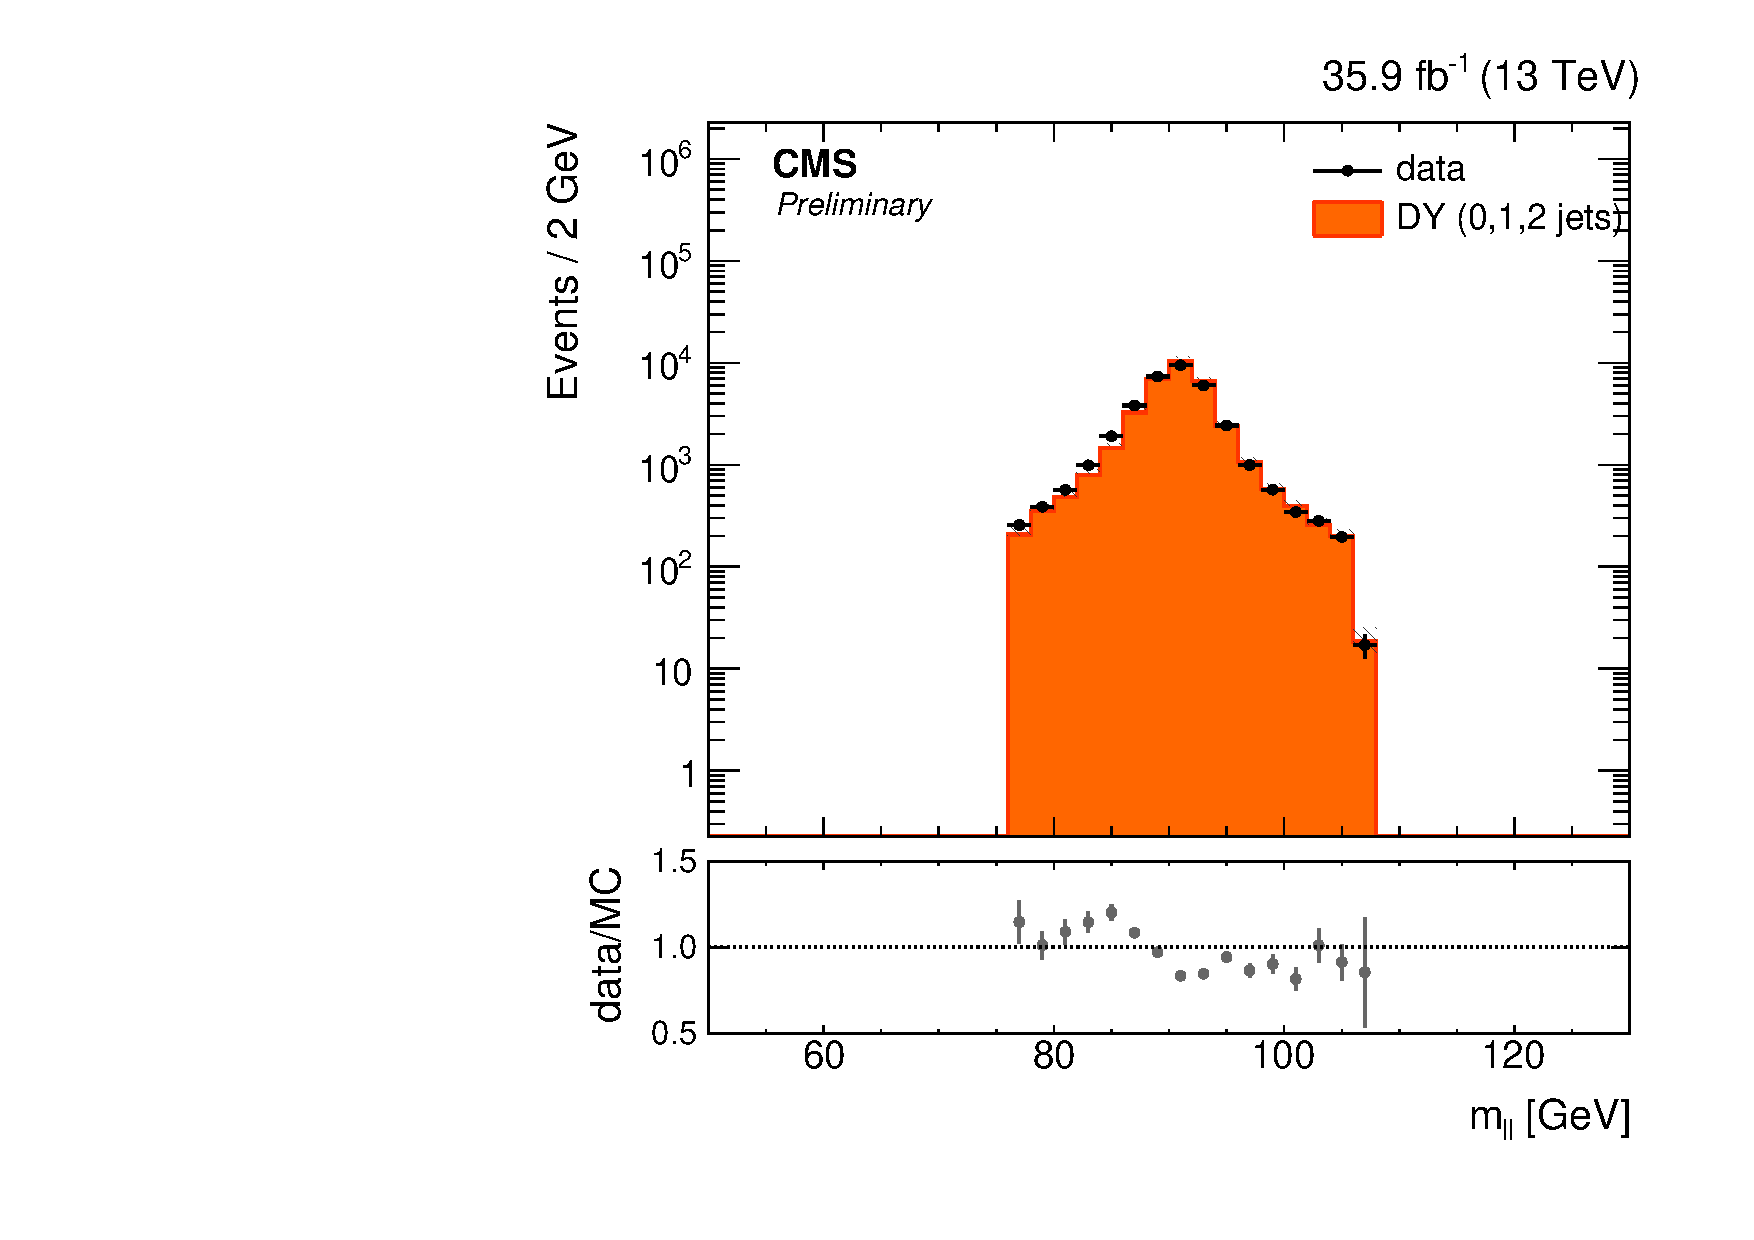
\includegraphics[width=0.4\textwidth]{figs/dilep_mass_em_bkg_sub_metbin1_ee.pdf}}
    \subfloat[$75\:\GeV<\ptmiss<100\:\GeV$]     {\label{subfig:Zpeak_metbin2_ee}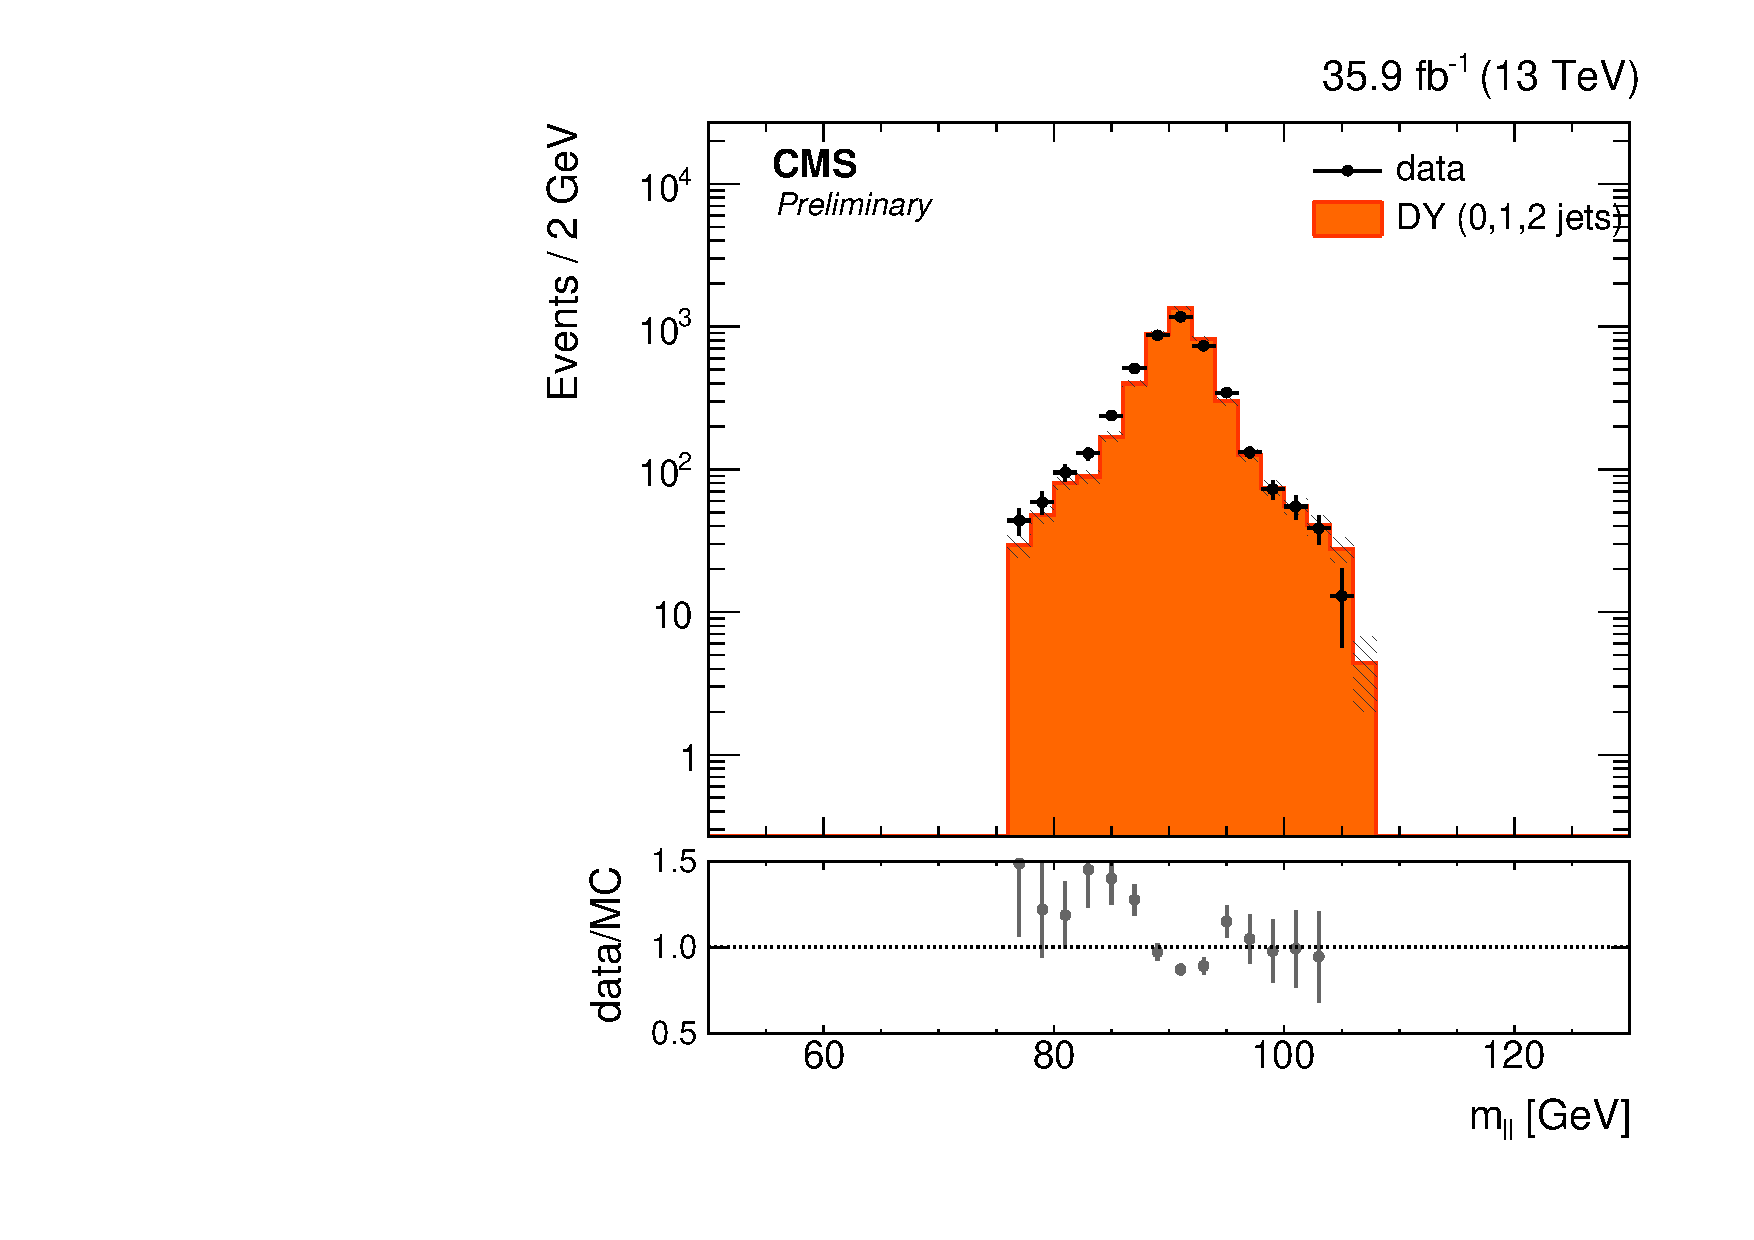
\includegraphics[width=0.4\textwidth]{figs/dilep_mass_em_bkg_sub_metbin2_ee.pdf}} \\
    \subfloat[$100\:\GeV<\ptmiss<150\:\GeV$]    {\label{subfig:Zpeak_metbin3_ee}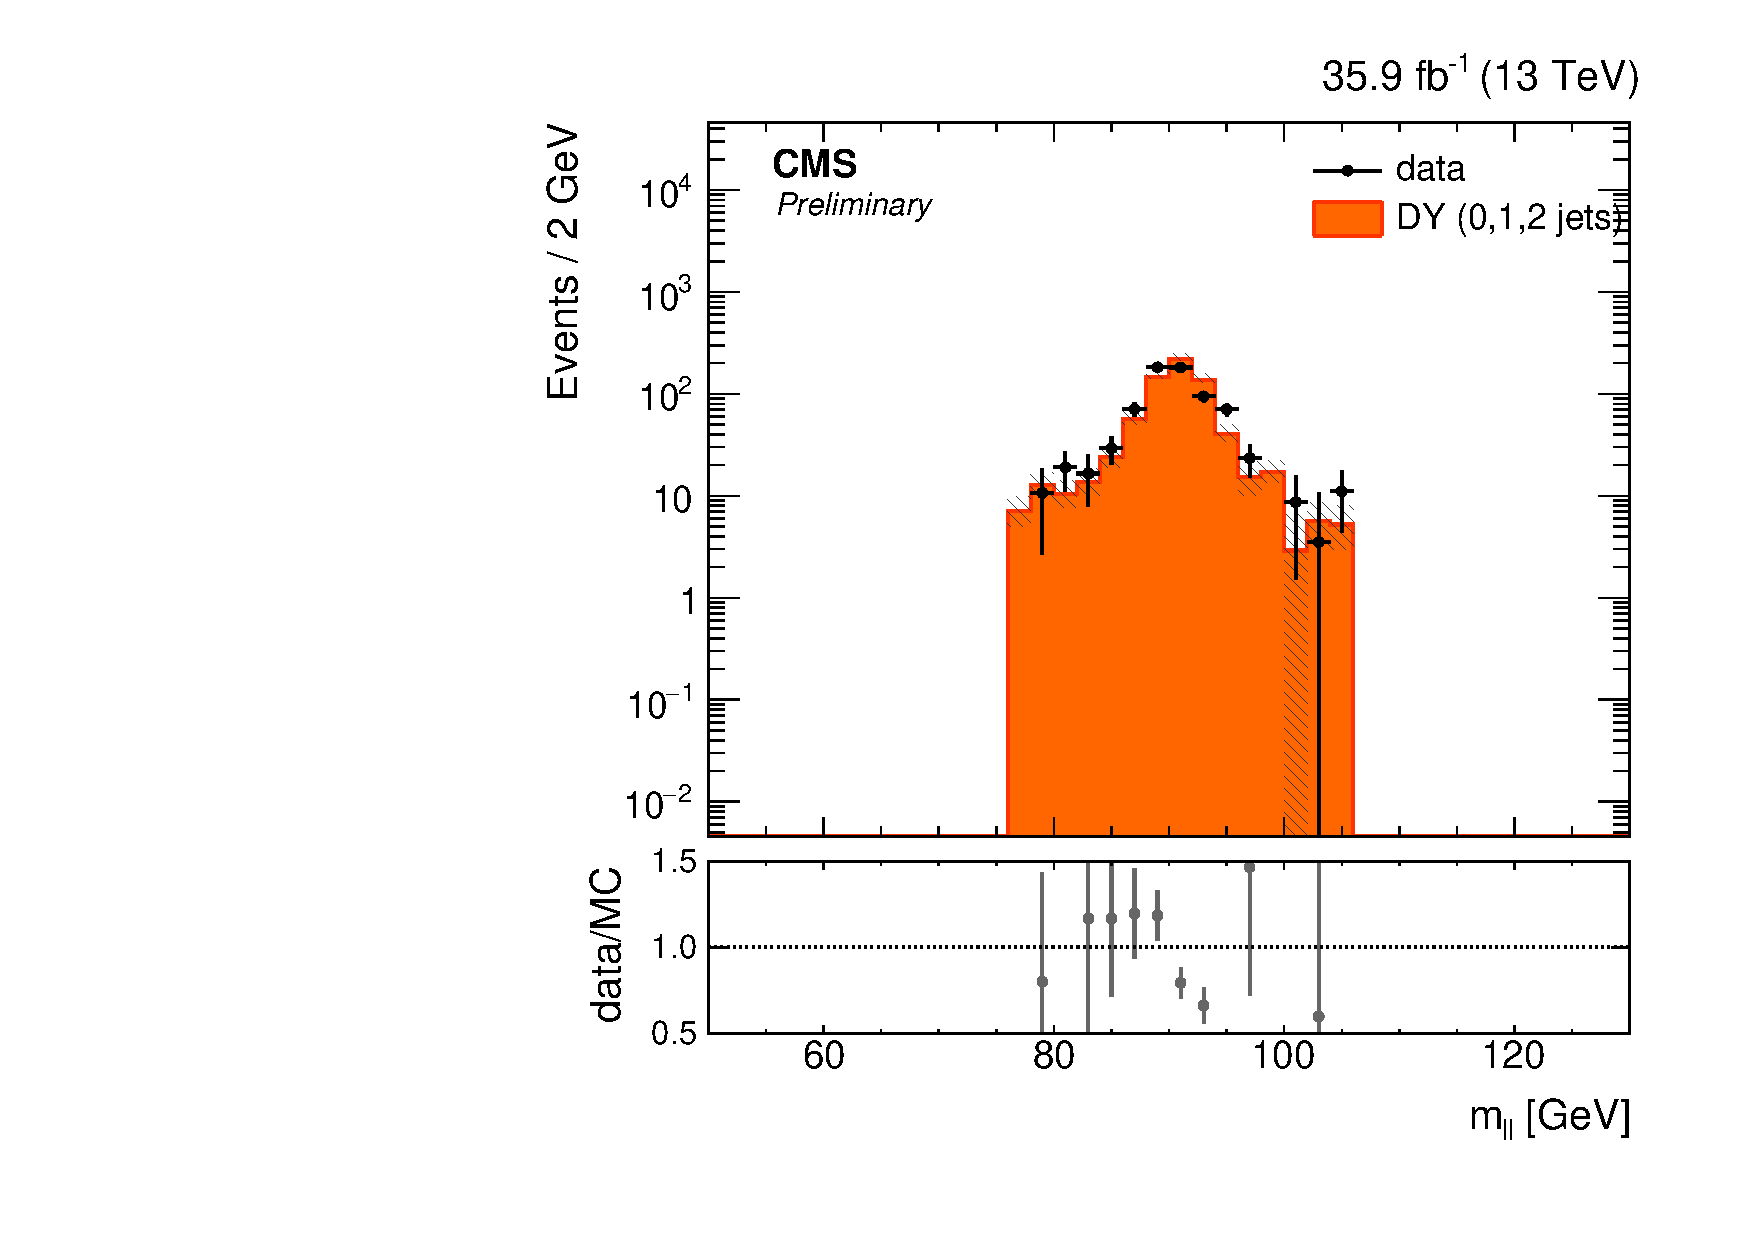
\includegraphics[width=0.4\textwidth]{figs/dilep_mass_em_bkg_sub_metbin3_ee.pdf}}
    \subfloat[$150\:\GeV<\ptmiss<1000\:\GeV$]   {\label{subfig:Zpeak_metbin4_ee}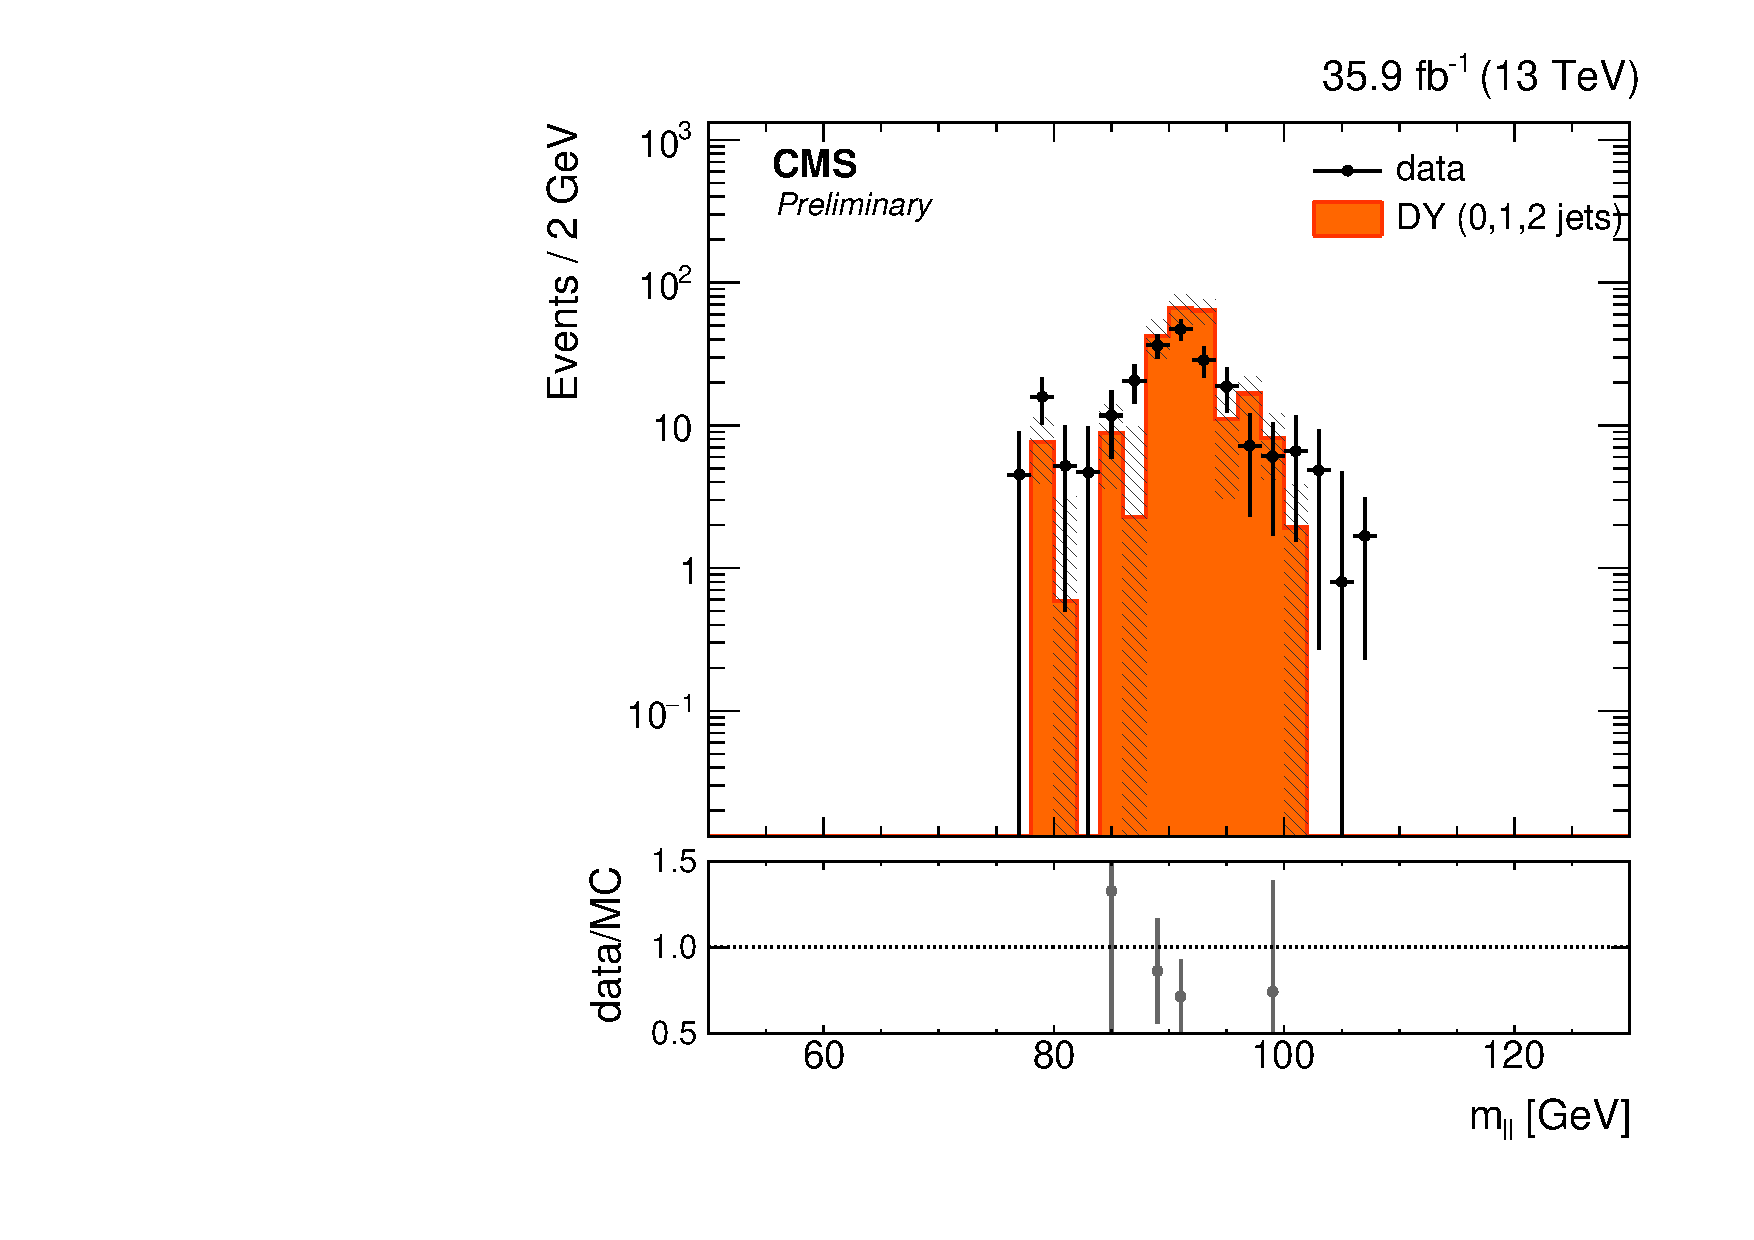
\includegraphics[width=0.4\textwidth]{figs/dilep_mass_em_bkg_sub_metbin4_ee.pdf}}
    \caption{Z peak in data and MC after subtraction of non-Drell-Yan contribution estimate from opposite-flavor data events in the $ee$ channel for various $\ptmiss$ bins.}
    \label{fig:Zpeak_ee}
  \end{center}
  \label{tab:Rinout_SF_mm}
\end{figure}

\begin{figure}
  \begin{center}
    \subfloat[$50\:\GeV<\ptmiss<75\:\GeV$]  {\label{subfig:Zpeak_metbin1_mm}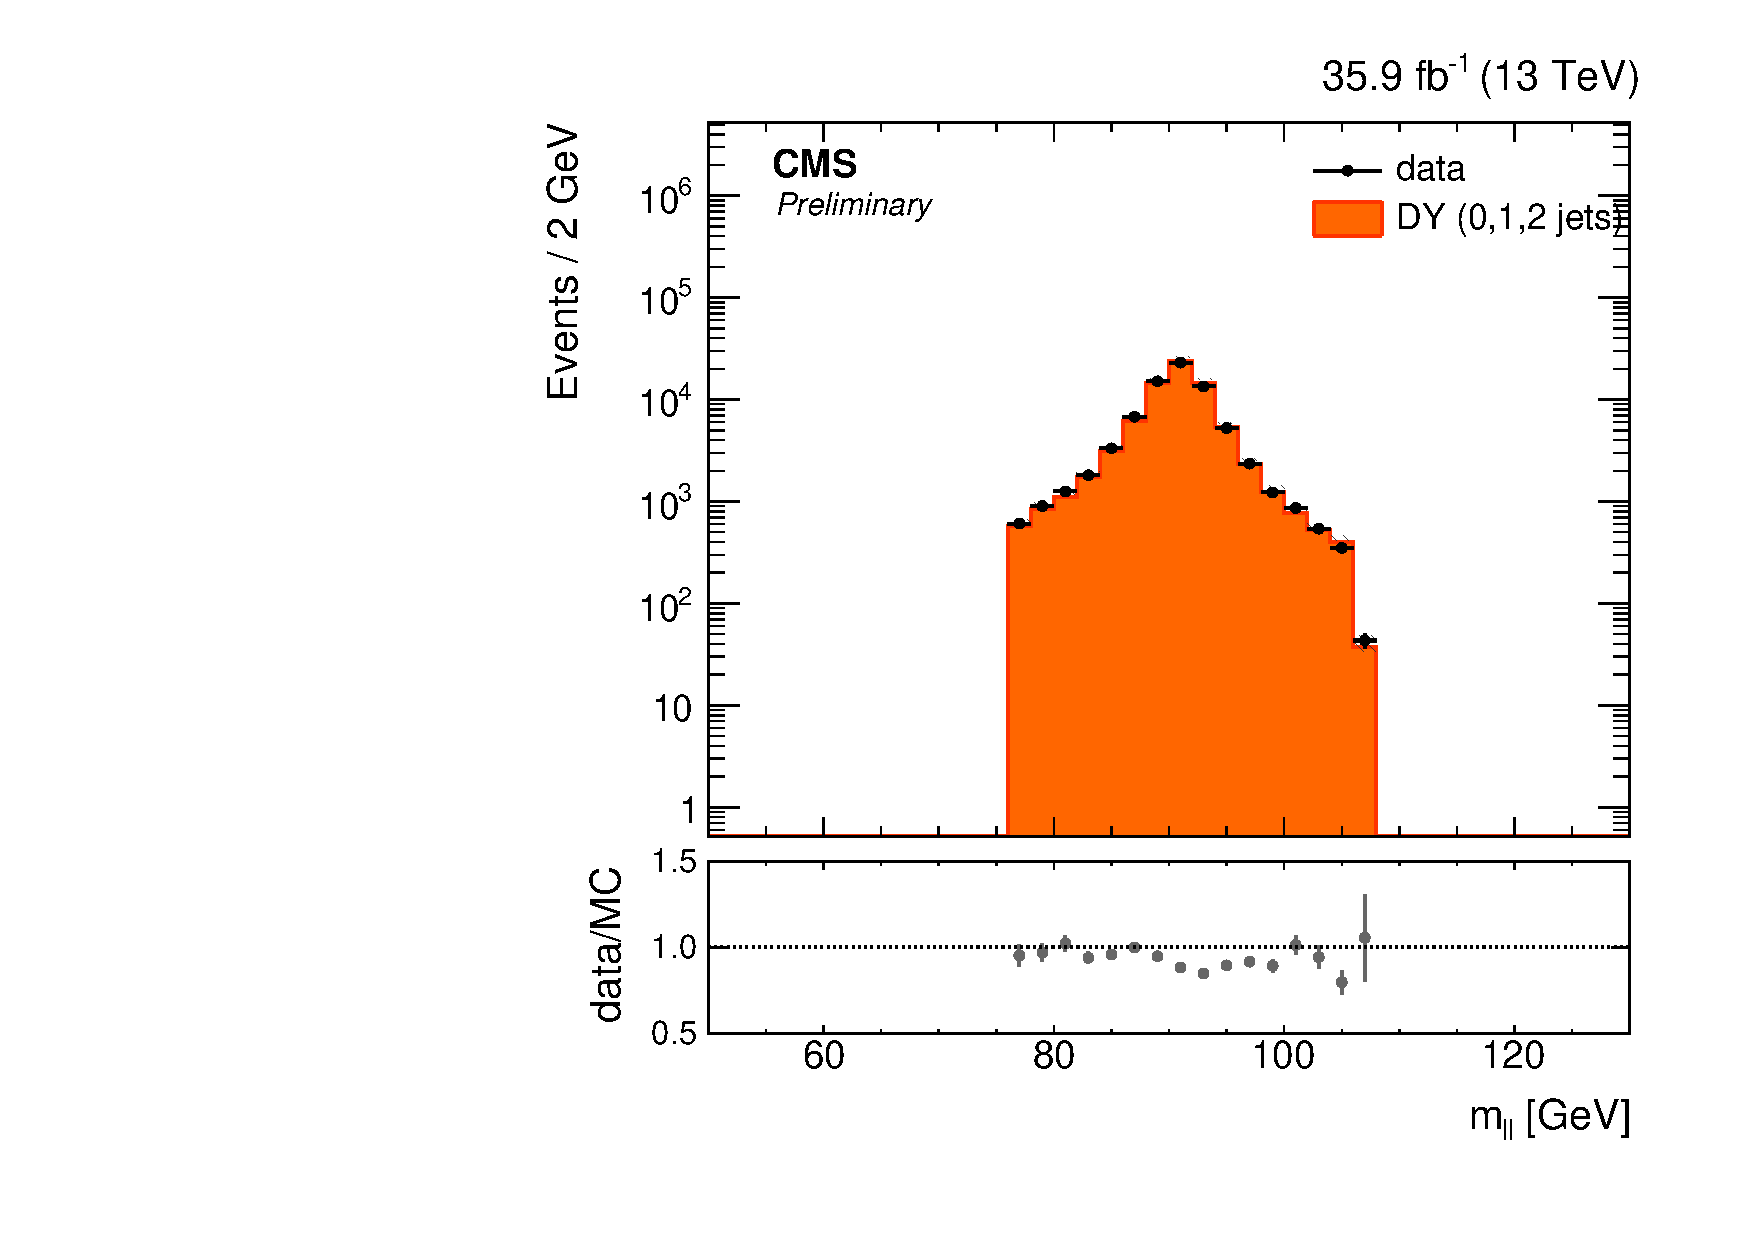
\includegraphics[width=0.4\textwidth]{figs/dilep_mass_em_bkg_sub_metbin1_mm.pdf}}
    \subfloat[$75\:\GeV<\ptmiss<100\:\GeV$] {\label{subfig:Zpeak_metbin2_mm}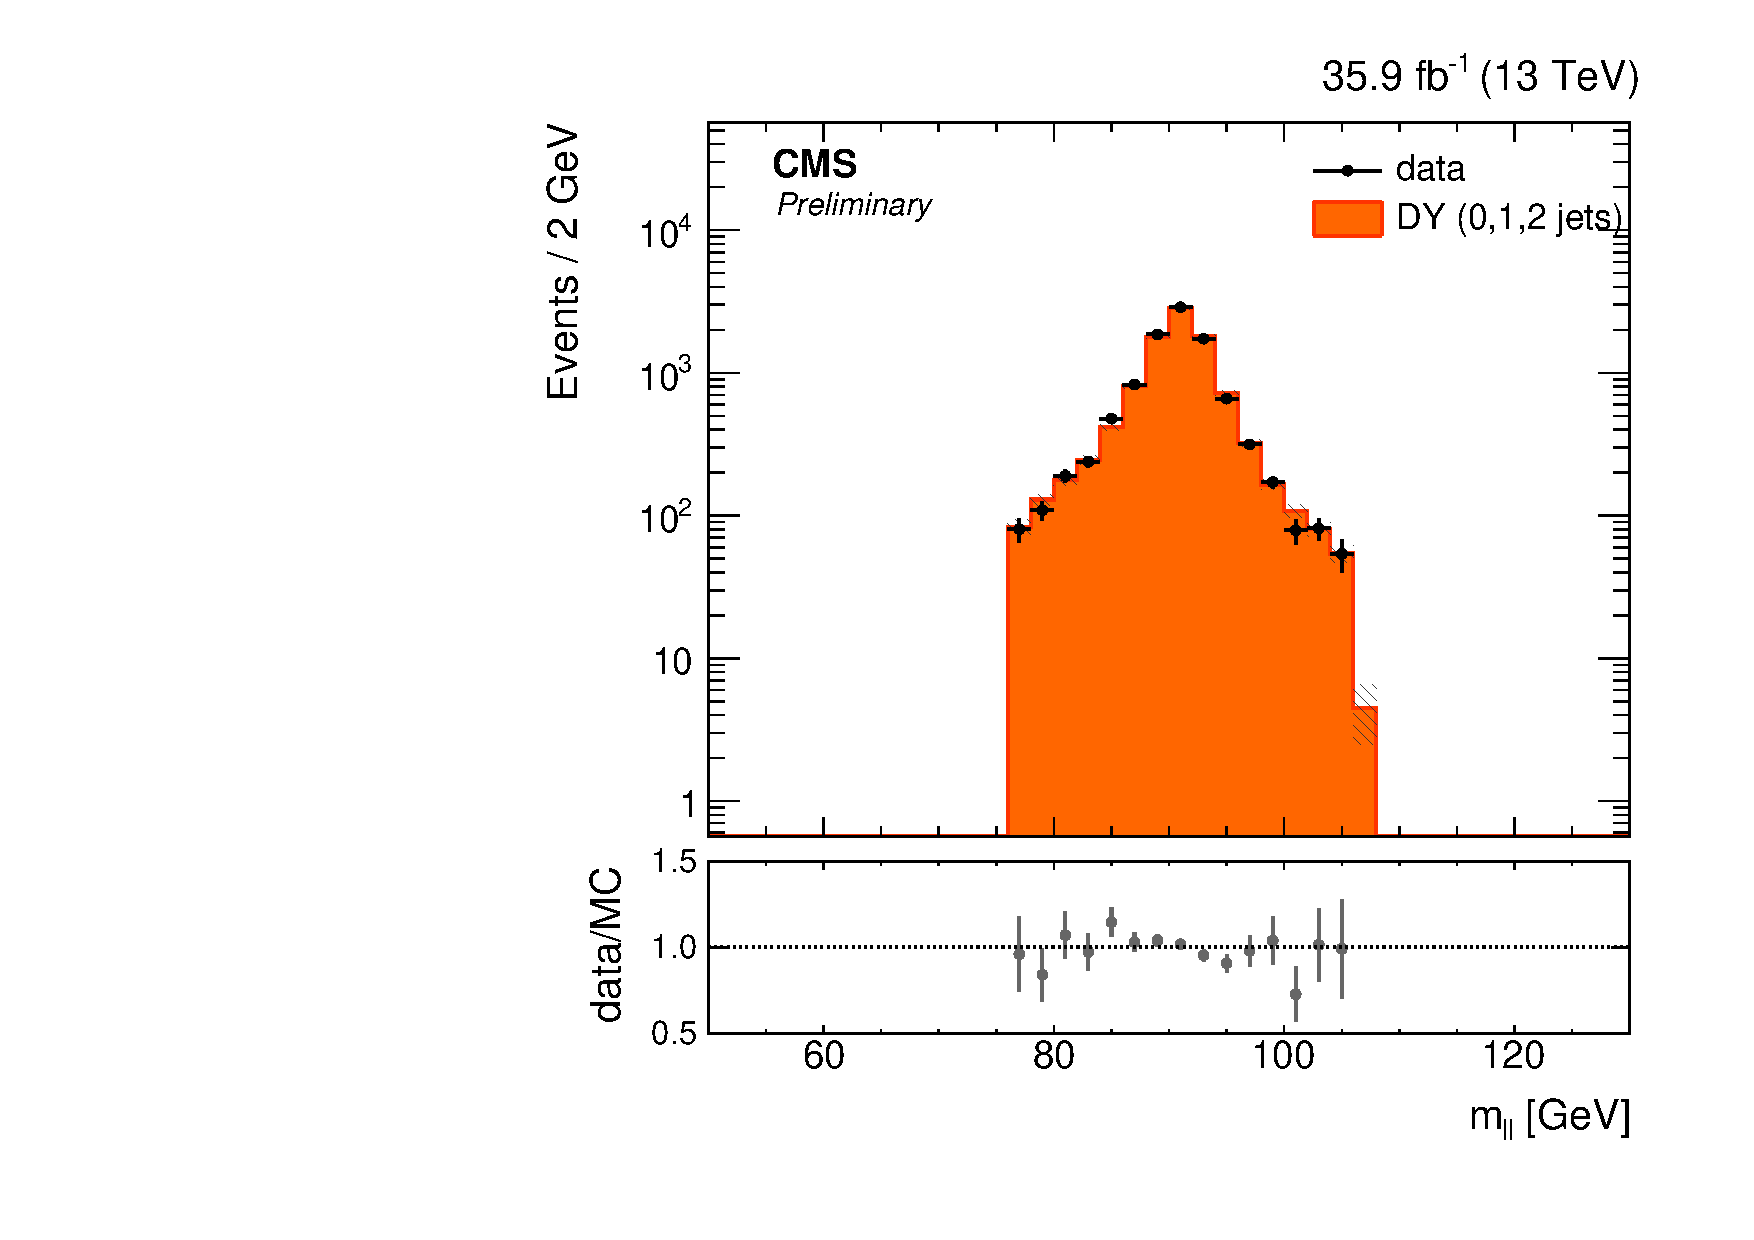
\includegraphics[width=0.4\textwidth]{figs/dilep_mass_em_bkg_sub_metbin2_mm.pdf}}\\
    \subfloat[$100\:\GeV<\ptmiss<150\:\GeV$]{\label{subfig:Zpeak_metbin3_mm}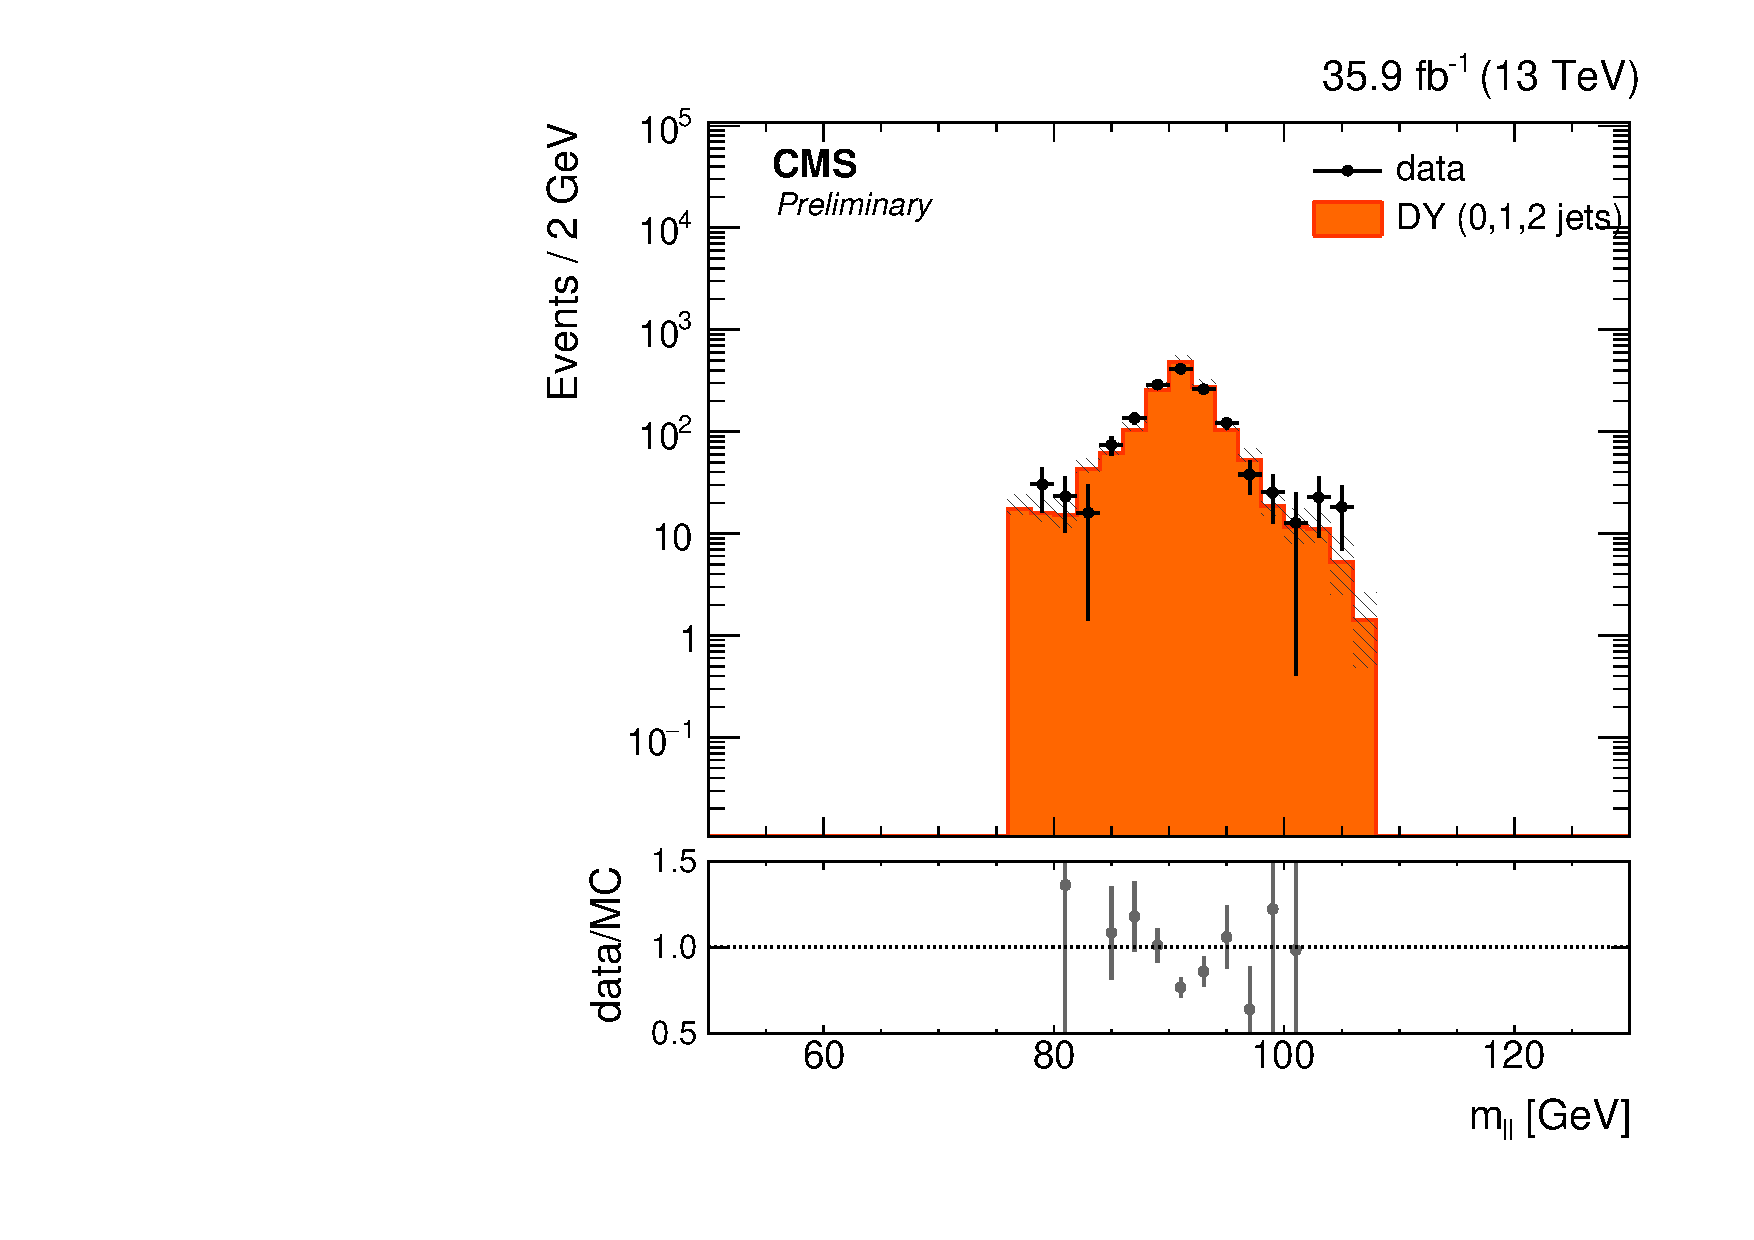
\includegraphics[width=0.4\textwidth]{figs/dilep_mass_em_bkg_sub_metbin3_mm.pdf}}
    \subfloat[$150\:\GeV<\ptmiss<1000\:\GeV$]{\label{subfig:Zpeak_metbin4_mm}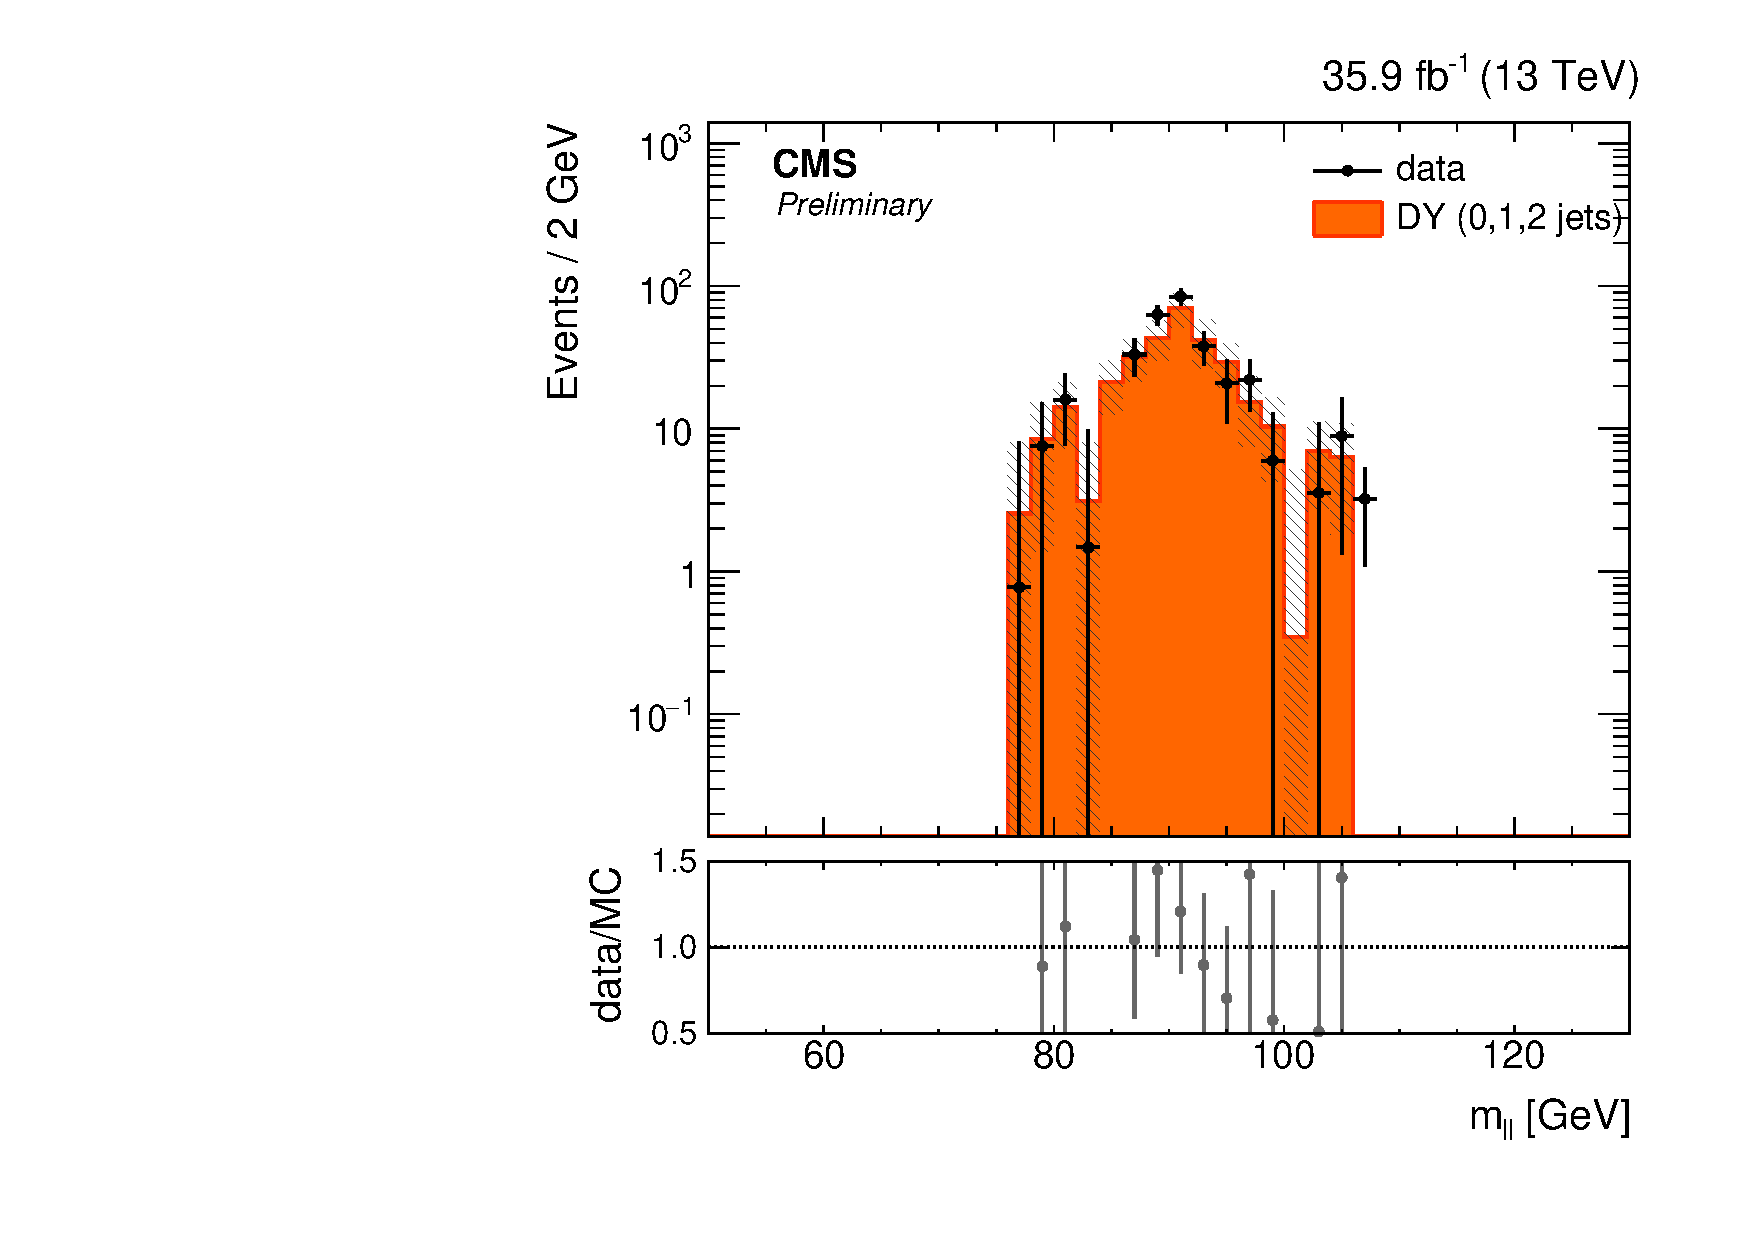
\includegraphics[width=0.4\textwidth]{figs/dilep_mass_em_bkg_sub_metbin4_mm.pdf}}
    \caption{Z peak in data and MC after subtraction of non-Drell-Yan contribution estimate from opposite-flavor data events in the $\mu\mu$ channel for various $\ptmiss$ bins.}
    \label{fig:Zpeak_mm}
  \end{center}
\end{figure}

\begin{figure}
  \centering
  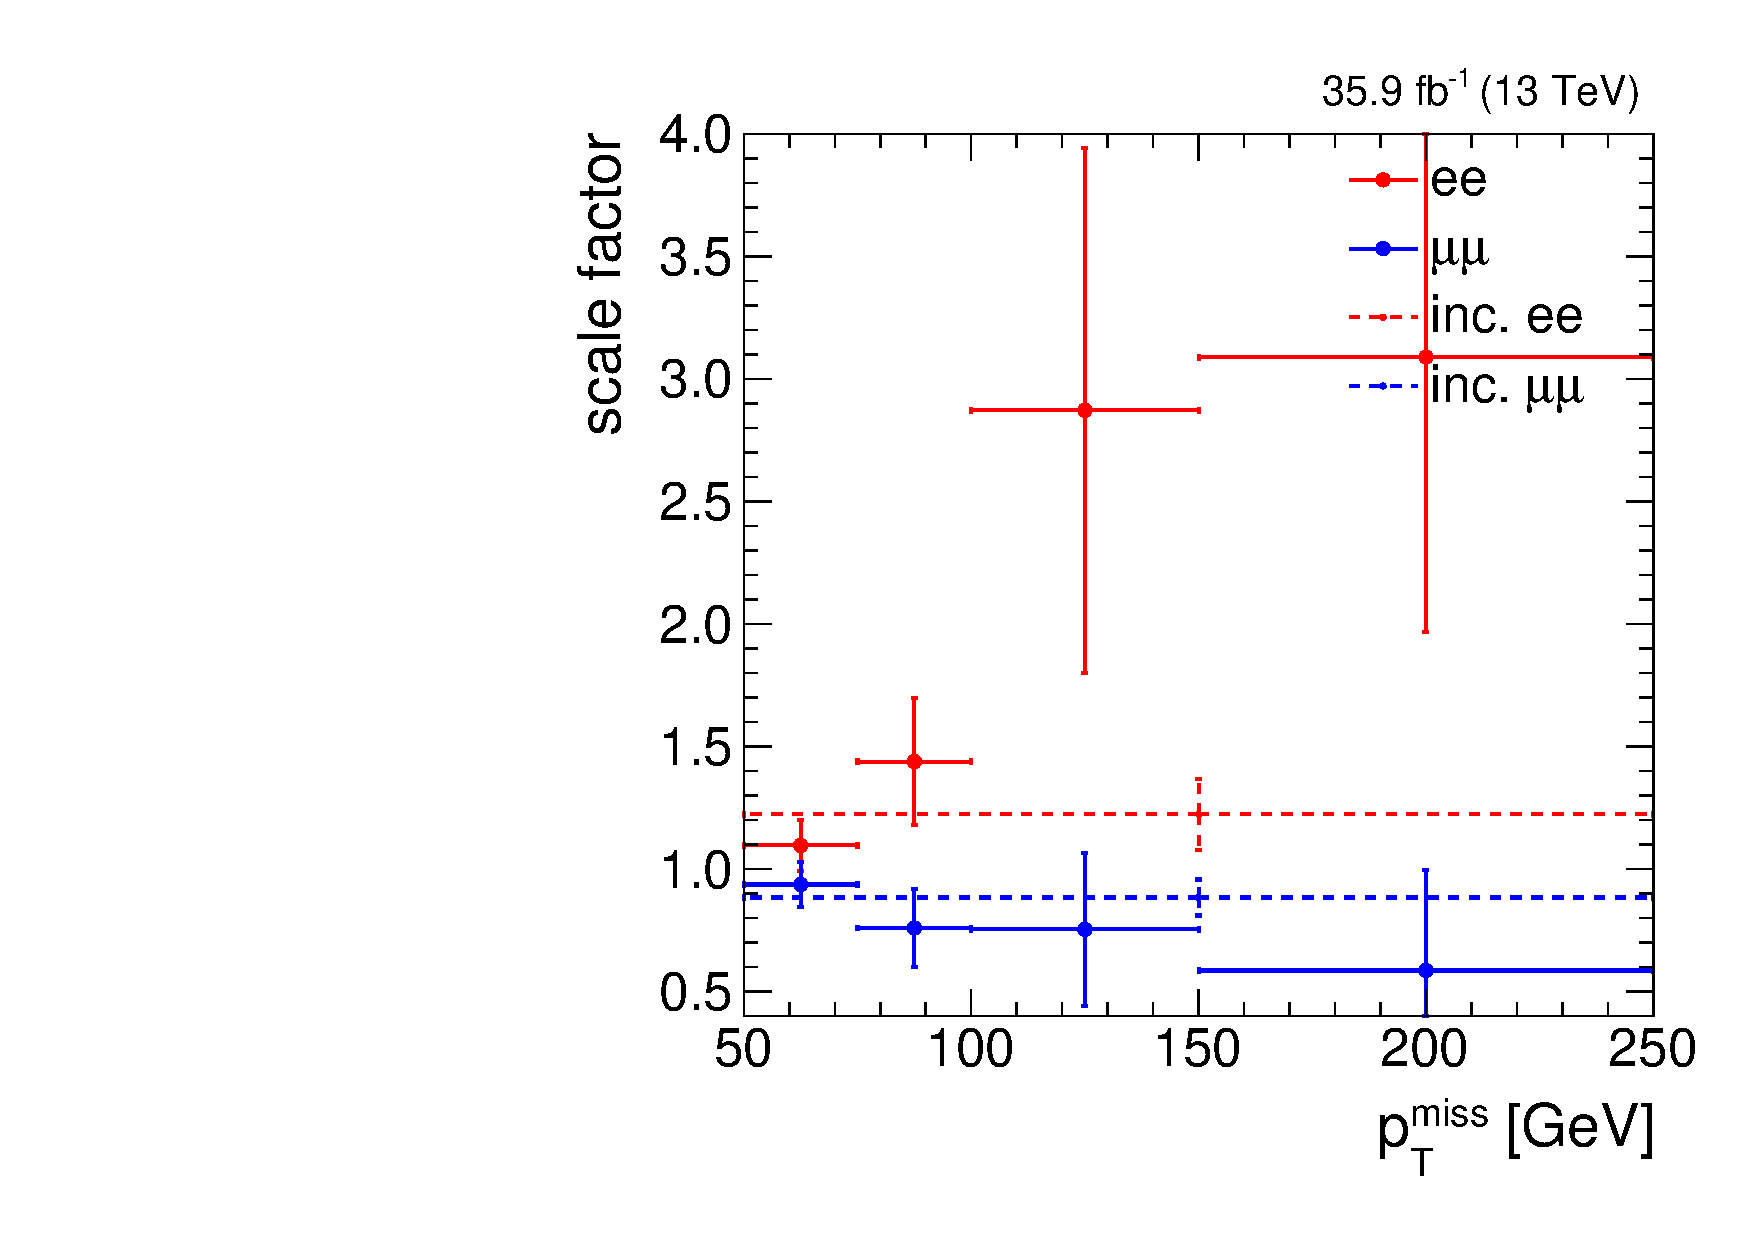
\includegraphics[width=0.48\textwidth]{figs/metbinned_Rinout_SFs.pdf}       
  \caption{Data/MC scale factors binned in $\ptmiss$ applied to MC events used for the estimate of the Drell-Yan normalization in the dilepton channel signal regions.}
  \label{fig:RinoutSFs}
\end{figure}

\clearpage

%%------------------------- Fakes -------------------------%%  
\section{Fake lepton background}
\label{sec:fakes}
\begin{figure}
  \subfloat[][\Wjets]{\label{fig:wjets}
    \feynmandiagram[vertical=b to c]{
      a [particle=\(u\)] -- [fermion] b -- [fermion] c -- [fermion] d [particle=\(\bar{d}\)],
      b -- [boson, edge label=\(W^{+}\)] f,
      e [particle=\(\ell^{+}\)] -- [fermion] f -- [fermion] g [particle=\(\nu_{\ell}\)],
      c -- [gluon, edge label=\(g\)] i,
      j [particle=\(\bar{b}\)] -- [fermion] i -- [fermion] h [particle=\(b\)],
      %        g -- [opacity=0.0001] h,
      %        a -- [opacity=0.0001] d,
      f -- [opacity=0.0001] i,
    };
  } 
  \hspace{1.0 cm}
  \subfloat[][$t\bar{t}(1\ell)$]{\label{fig:tt1l}
    \feynmandiagram[horizontal=b to c]{
      a [particle=\(g\)] -- [gluon] b -- [gluon] c,
      d [particle=\(g\)] -- [gluon] b,
      e -- [fermion, edge label=\(\bar{t}\)] c,
      g [particle=\(\bar{b}\)] -- [fermion] e,
      e -- [boson, edge label=\(W^-\)] h,
      c -- [fermion, edge label=\(t\)] f,
      e -- [opacity=0.0001] f,
      f -- [fermion] i [particle=\(b\)],
      f -- [boson, edge label'=\(W^+\)] j,
      k [particle=\(\bar{\nu}_{\ell}\)] -- [fermion] h -- [fermion] l [particle=\(\ell^-\)],
      m [particle=\(\bar{q}\)] -- [fermion] j -- [fermion] n [particle=\(q\)],
    };
  }
  \caption{Examples of~\protect\subref{fig:wjets} \Wjets, and ~\protect\subref{fig:tt1l} semileptonic \ttbar that contribute to the fake lepton background.}
  \label{fig:fakes_feyn}
\end{figure}


Another type of reducible background, the fake (or non-prompt) lepton background, is also estimated using observed events. Processes which are expected to contain only one prompt electron or muon in the final state may pass the signal region selection as described in Sec.~\ref{sec:selection} by a jet-induced faking of a second lepton. Namely, processes such as \Wjets, semileptonic decays of \ttbar and tW associated production, and leptonic single top decays, a few of which are shown in~\FigureRef{fig:fakes_feyn}, comprise the fake lepton background processes. 

The data-driven technique used to estimate the relative contribution of fake lepton backgrounds in the signal regions is based on the measurement of the fake rate. This rate is obtained from a sample in data which is enriched in QCD multijet events. Very loose working points for an electron object and muon object are define; these are called ``fake-able objects'' (``FO'') and their definitions are found under the heading ``FO WP'' in Tables~\ref{tab:ele_wp} and~\ref{tab:muon_wp} for electrons and muons respectively.

The method has two main steps,
\begin{enumerate}
\item \textbf{Measurement:} in a QCD enriched sample in data, measure the probability of a ``FO'' to pass ``Tight'' lepton selection: the ``fake rate''
\item \textbf{Application:} in a sample consisting of one ``Tight'' lepton and one ``FO'' that fails ``Tight'' selection, use the fake rate to estimate the background in the signal region
\end{enumerate}

\subsection{Fake rate measurement}
\label{subsec:fr_measure}
To obtain a sample enriched in jet-induced fakes in order to perform the fake rate measurement, the following selection is applied,
\begin{itemize}
\item Event passes one of the following triggers:
  \begin{itemize}
  \item HLT\_Ele$[12, 23]$\_CaloIdM\_TrackIdM\_PFJet30
  \item HLT\_Ele$[12, 23]$\_CaloIdL\_TrackIdL\_IsoVL\_PFJet30
  \item HLT\_Mu$[8, 17]$\_TrkIsoVVL
  \end{itemize}
\item there is exactly one ``FO'' in the event, matched to the trigger that fired
\item \ptmiss<40\:\GeV
\item $M_{T}<35\:\GeV$
\item at least one jet with $\pt>30\:\GeV$ and $|\eta|<4$
\item $\Delta\phi>2$ between the leading jet in the event and the ``FO''
\end{itemize}
The cuts are chosen to suppress the \Wjets contribution (i.e. the low $M_{T}$ requirement), and to enhance the multi-jet QCD contribution. Even then, the level of contamination from electroweak processes (\Wjets, \Zjets, \ttbar) in this sample ranges from $10\%$ at low \pt to $70\%$ at high \pt. The contamination is thus significant, particularly in the measurement sample for muon ``FO'', that a subtraction of prompt, real leptons must be done (based on expectations from simulation). The fake rate (FR) is defined as the efficiency of a ``FO'' to pass ``Tight'' requirements,
\begin{equation}
  \text{FR}_{ij} = \Big[\frac{\left(N^{\text{data}}_{Tight} - N^{\text{EWK}}_{Tight}\right)}{\left(N^{\text{data}}_{FO} - N^{\text{EWK}}_{FO}\right)}\Big]_{i=\eta\,j=\pt}
\end{equation}
The measured fake rates are listed in Tables~\ref{tab:ele_fr} and~\ref{tab:muon_fr}. The fake rates depend more strongly on \eta than on \pt as shown in Fig.~\ref{fig:ele_fr_plots} and Fig.~\ref{fig:muon_fr_plots}.

\begin{table}[!ht]
\centering
\scalebox{0.9}
{
\begin{tabular}{|c|c|c|c|c|c|}
\hline
                & $0.0 < |\eta| < 0.5$ & $0.5 < |\eta| < 1.0$ & $1.0 < |\eta| < 1.5$ & $1.5 < |\eta| < 2
.0$ & $2.0 < |\eta| < 2.5$ \\
\hline
$10 < \pt < 15$ &  $0.063 \pm  0.008$  & $ 0.088 \pm  0.009$  &  $0.121 \pm  0.008$  &  $0.181 \pm  0.00
9$  &  $0.176 \pm  0.012$ \\
\hline  
$15 < \pt < 20$ &  $0.085 \pm  0.003$  & $ 0.085 \pm  0.003$  &  $0.106 \pm  0.003$  &  $0.164 \pm  0.00
4$  &  $0.153 \pm  0.005$ \\
\hline
$20 < \pt < 25$ & $ 0.062 \pm  0.008$  &  $0.059 \pm  0.007$  &  $0.080 \pm  0.009$  &  $0.131 \pm  0.010$  &  $0.148 \pm  0.012$ \\
\hline 
$25 < \pt < 30$ &  $0.073 \pm  0.011$  &  $0.078 \pm  0.078$  &  $0.090 \pm  0.011$  &  $0.140 \pm  0.012$  &  $0.162 \pm  0.012$ \\
\hline
$\pt > 30$      &  $0.065 \pm  0.007$  &  $0.091 \pm  0.008$  &  $0.089 \pm  0.007$  &  $0.169 \pm  0.008$  &  $0.190 \pm  0.008$ \\
\hline    
\end{tabular}   
}
\caption{Electron fake rates}
\label{tab:ele_fr}
\end{table}

\begin{table}[!ht]
\centering
\scalebox{0.9}
{
\begin{tabular}{|c|c|c|c|c|c|}
\hline
                & $0.0 < |\eta| < 0.5$ & $0.5 < |\eta| < 1.0$ & $1.0 < |\eta| < 1.5$ & $1.5 < |\eta| < 2.0$ & $2.0 < |\eta| < 2.4$ \\
\hline
$10 < \pt < 15$ &  $0.192 \pm  0.004$  & $ 0.210 \pm  0.004$  &  $0.235 \pm  0.004$  &  $0.283 \pm  0.004$  &  $0.294 \pm  0.005$ \\
\hline
$15 < \pt < 20$ &  $0.202 \pm  0.001$  & $ 0.214 \pm  0.001$  &  $0.253 \pm  0.001$  &  $0.293 \pm  0.001$  &  $0.307 \pm  0.002$ \\
\hline
$20 < \pt < 25$ & $ 0.187 \pm  0.001$  &  $0.200 \pm  0.001$  &  $0.240 \pm  0.001$  &  $0.286 \pm  0.001$  &  $0.307 \pm  0.002$ \\
\hline 
$25 < \pt < 30$ &  $0.177 \pm  0.002$  &  $0.196 \pm  0.002$  &  $0.239 \pm  0.002$  &  $0.279 \pm  0.002$  &  $0.310 \pm  0.003$ \\
\hline
$\pt > 30$      &  $0.172 \pm  0.002$  &  $0.200 \pm  0.002$  &  $0.233 \pm  0.002$  &  $0.279 \pm  0.002$  &  $0.311 \pm  0.003$ \\
\hline    
\end{tabular}   
}
\caption{Muon fake rates}
\label{tab:muon_fr}
\end{table}

\begin{figure}[htbp!]
\begin{center}
  \subfloat[][fake rates vs. \pt]    {\label{subfig:fr_vs_pt_e}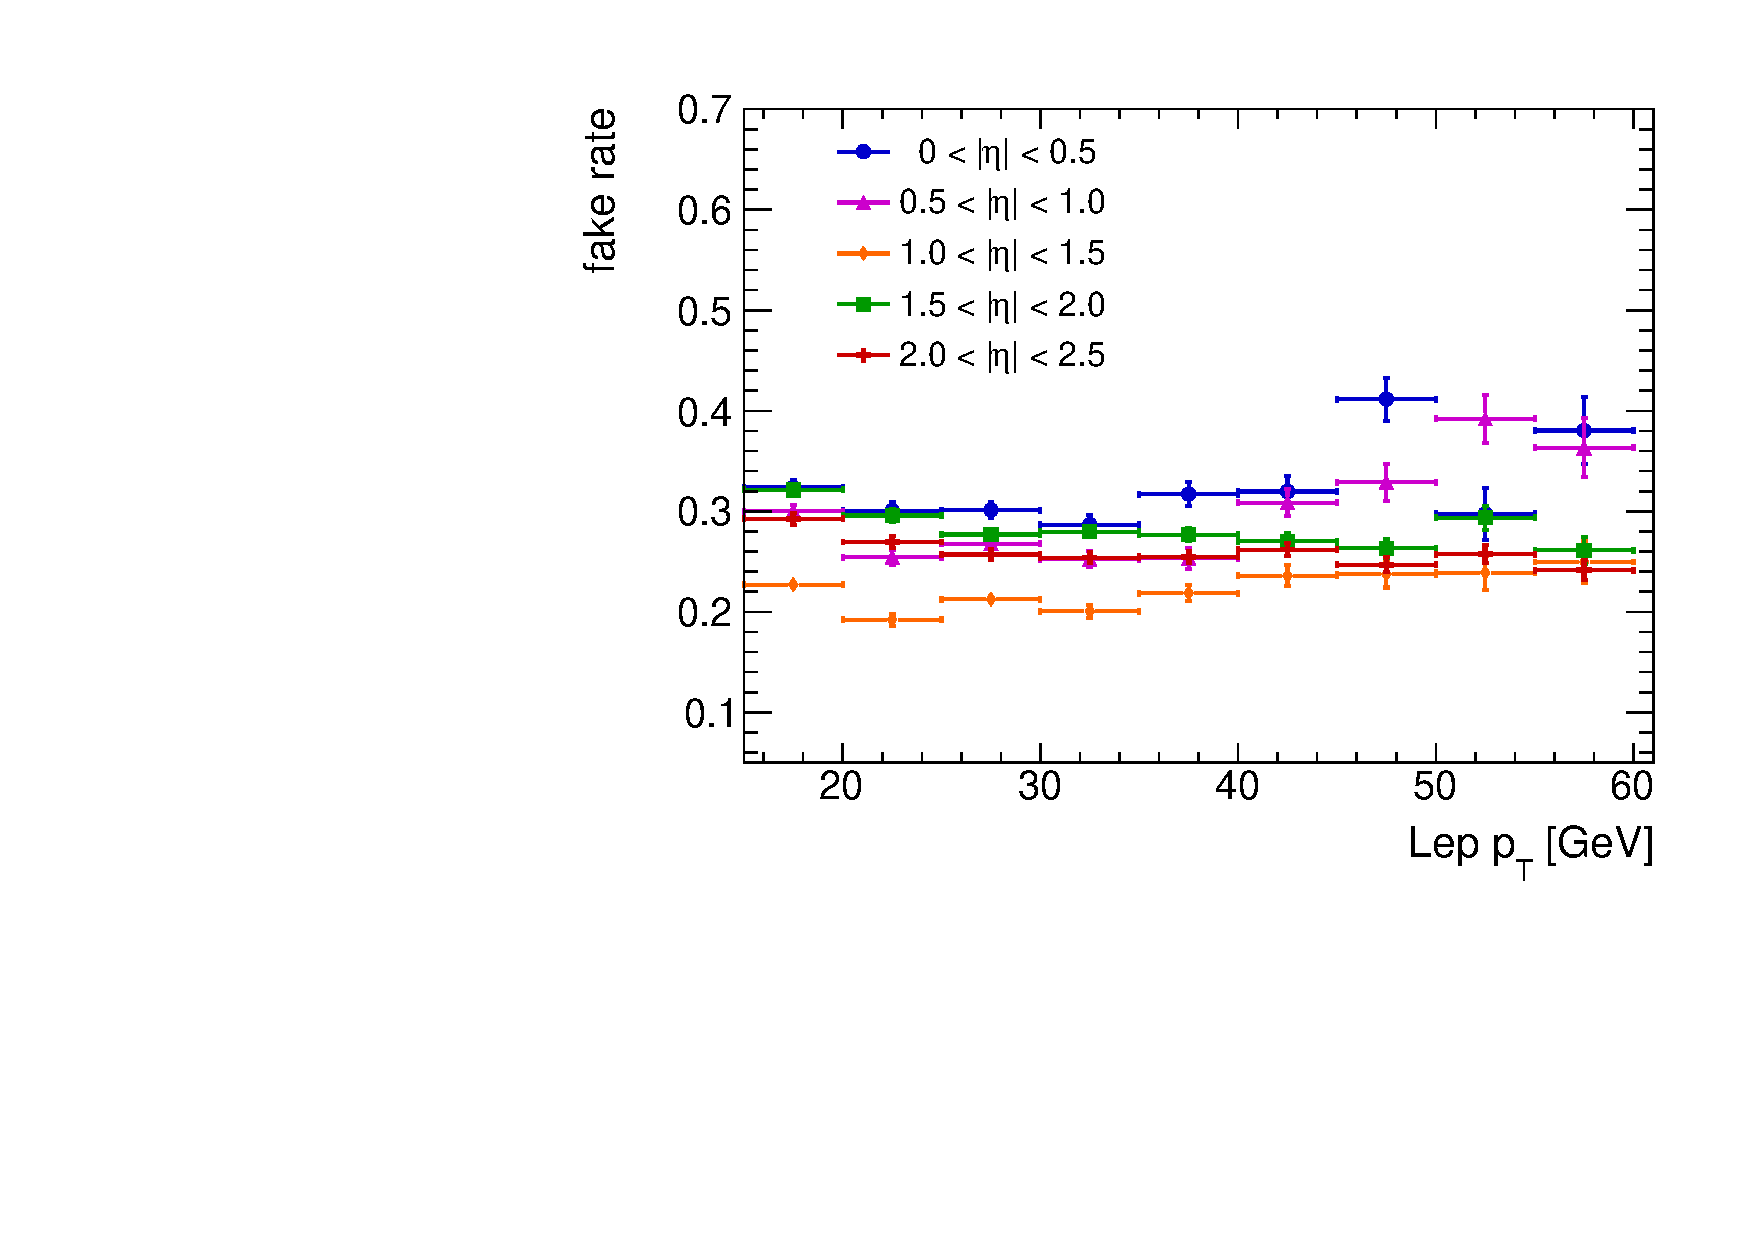
\includegraphics[width=0.45\textwidth]{figs/fakerate_v_pt_e.pdf}}
  \subfloat[][fake rates vs. $|\eta|$]  {\label{subfig:fr_vs_eta_e}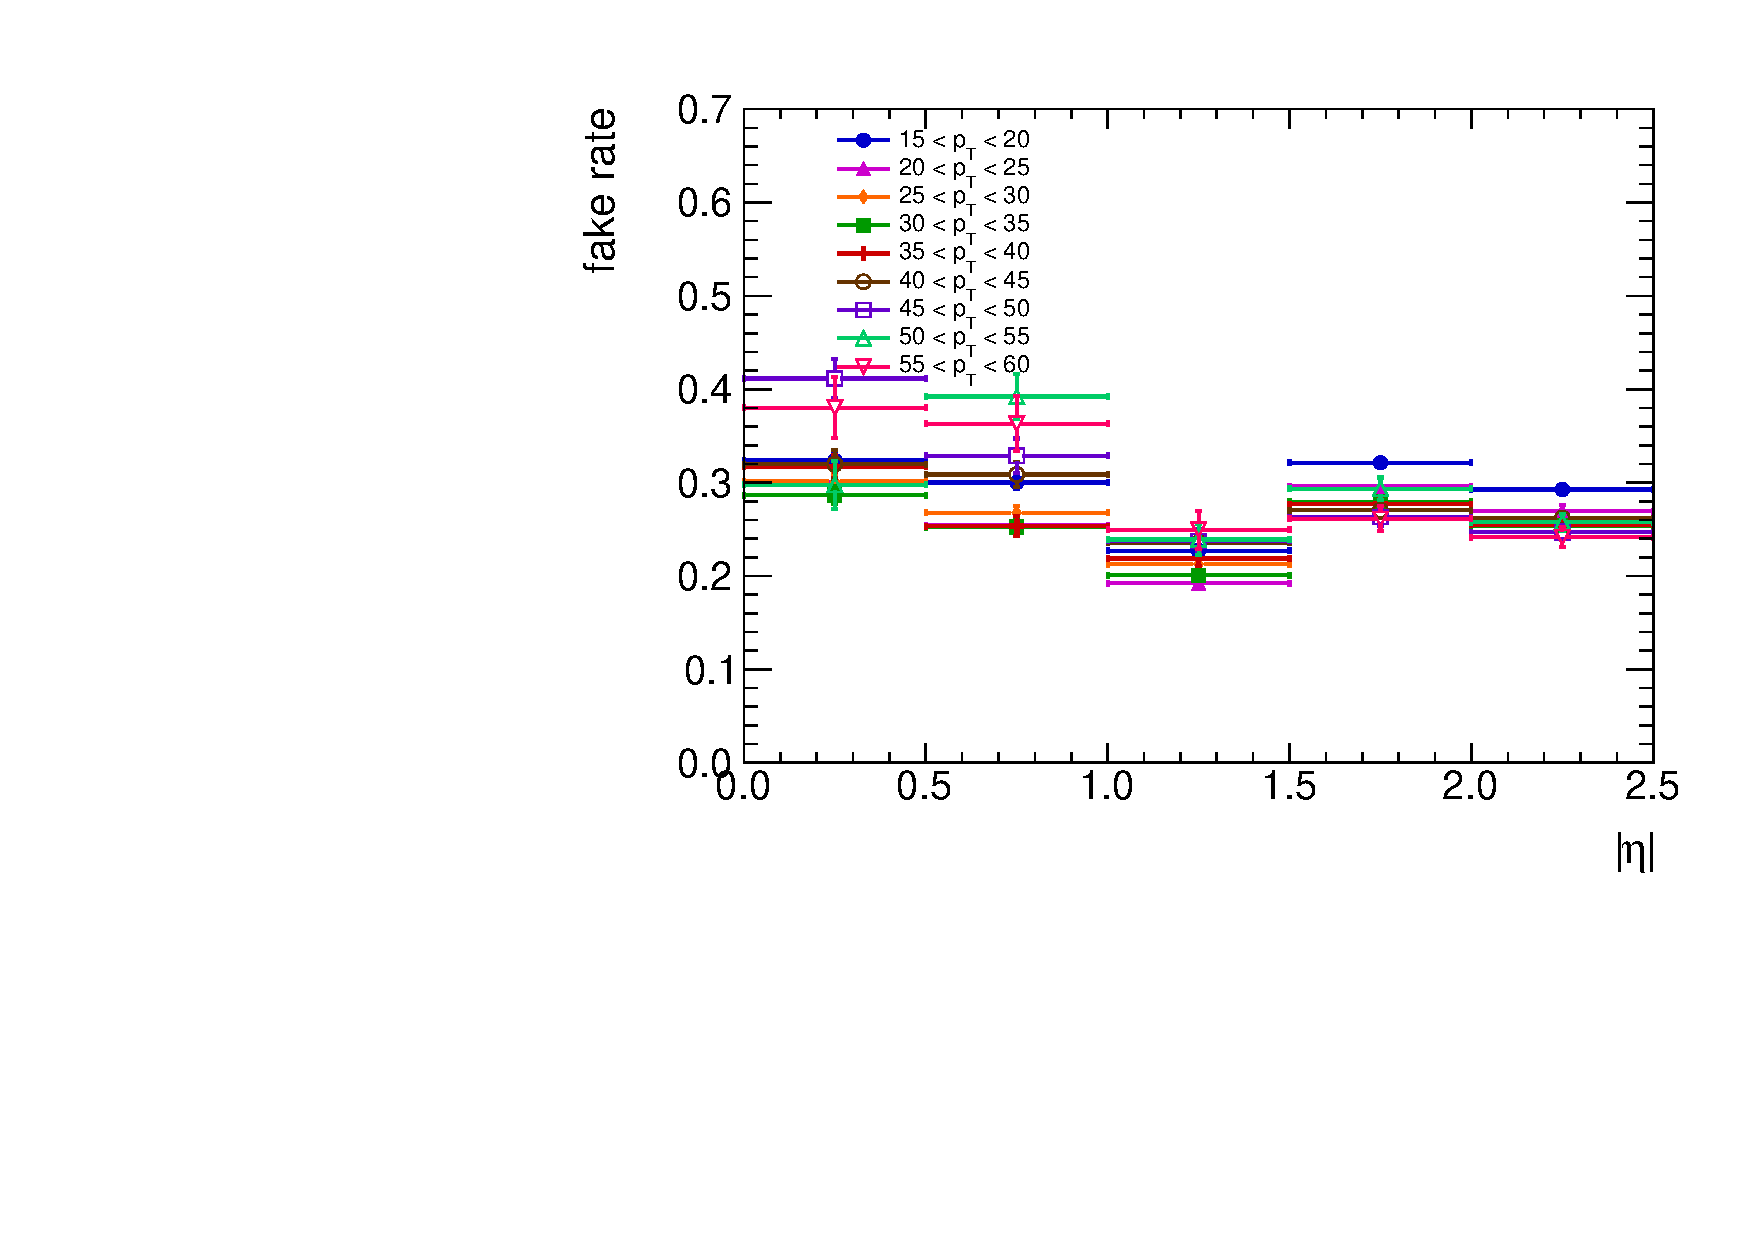
\includegraphics[width=0.45\textwidth]{figs/fakerate_v_eta_e.pdf}}
  \caption{Measured electron fake rates as a function of lepton ~\protect\subref{subfig:fr_vs_pt_e} $\pt$ and ~\protect\subref{subfig:fr_vs_eta_e} $|\eta|$.}
  \label{fig:ele_fr_plots}
\end{center}
\end{figure}

\begin{figure}[htbp!]
\begin{center}
  \subfloat[][fake rates vs. \pt]    {\label{subfig:fr_vs_pt_m}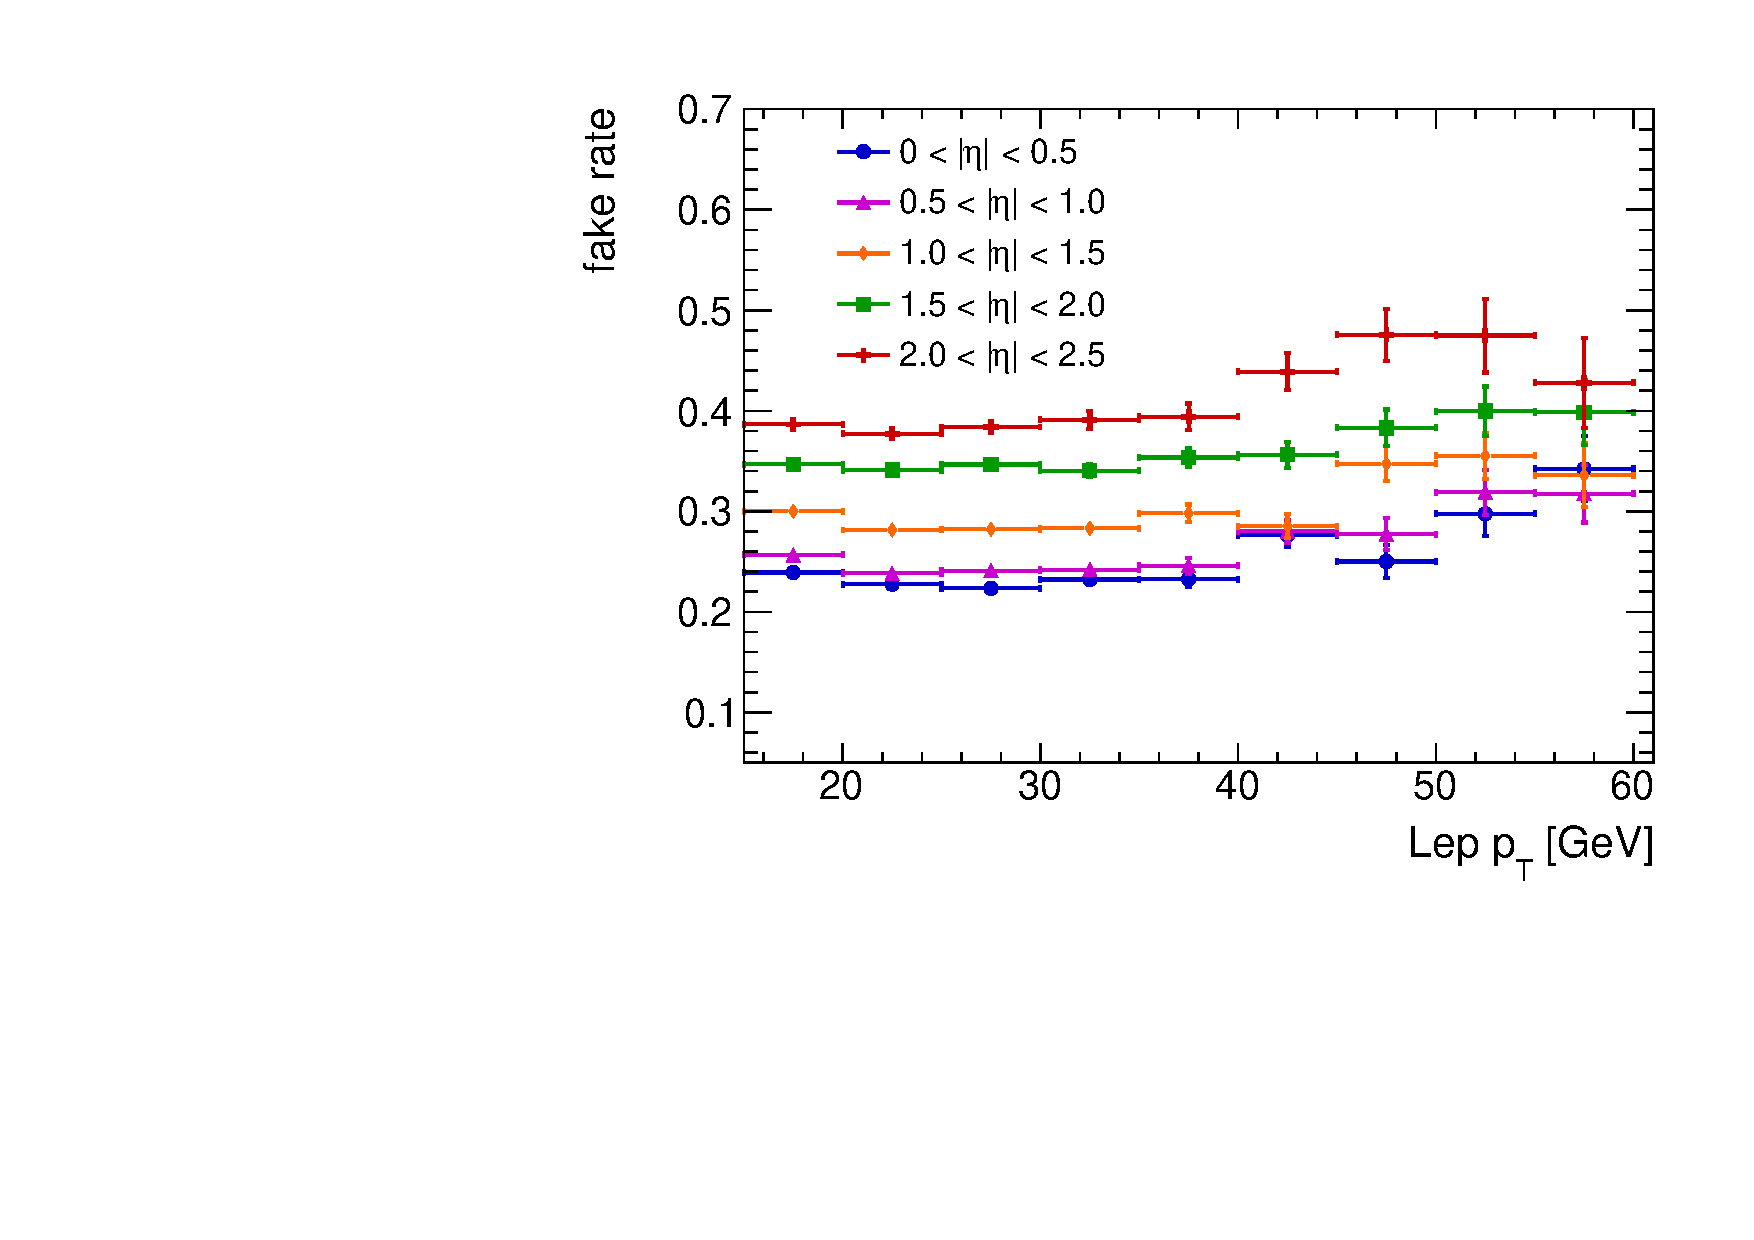
\includegraphics[width=0.45\textwidth]{figs/fakerate_v_pt_m.pdf}}
  \subfloat[][fake rates vs. $|\eta|$]  {\label{subfig:fr_vs_eta_m}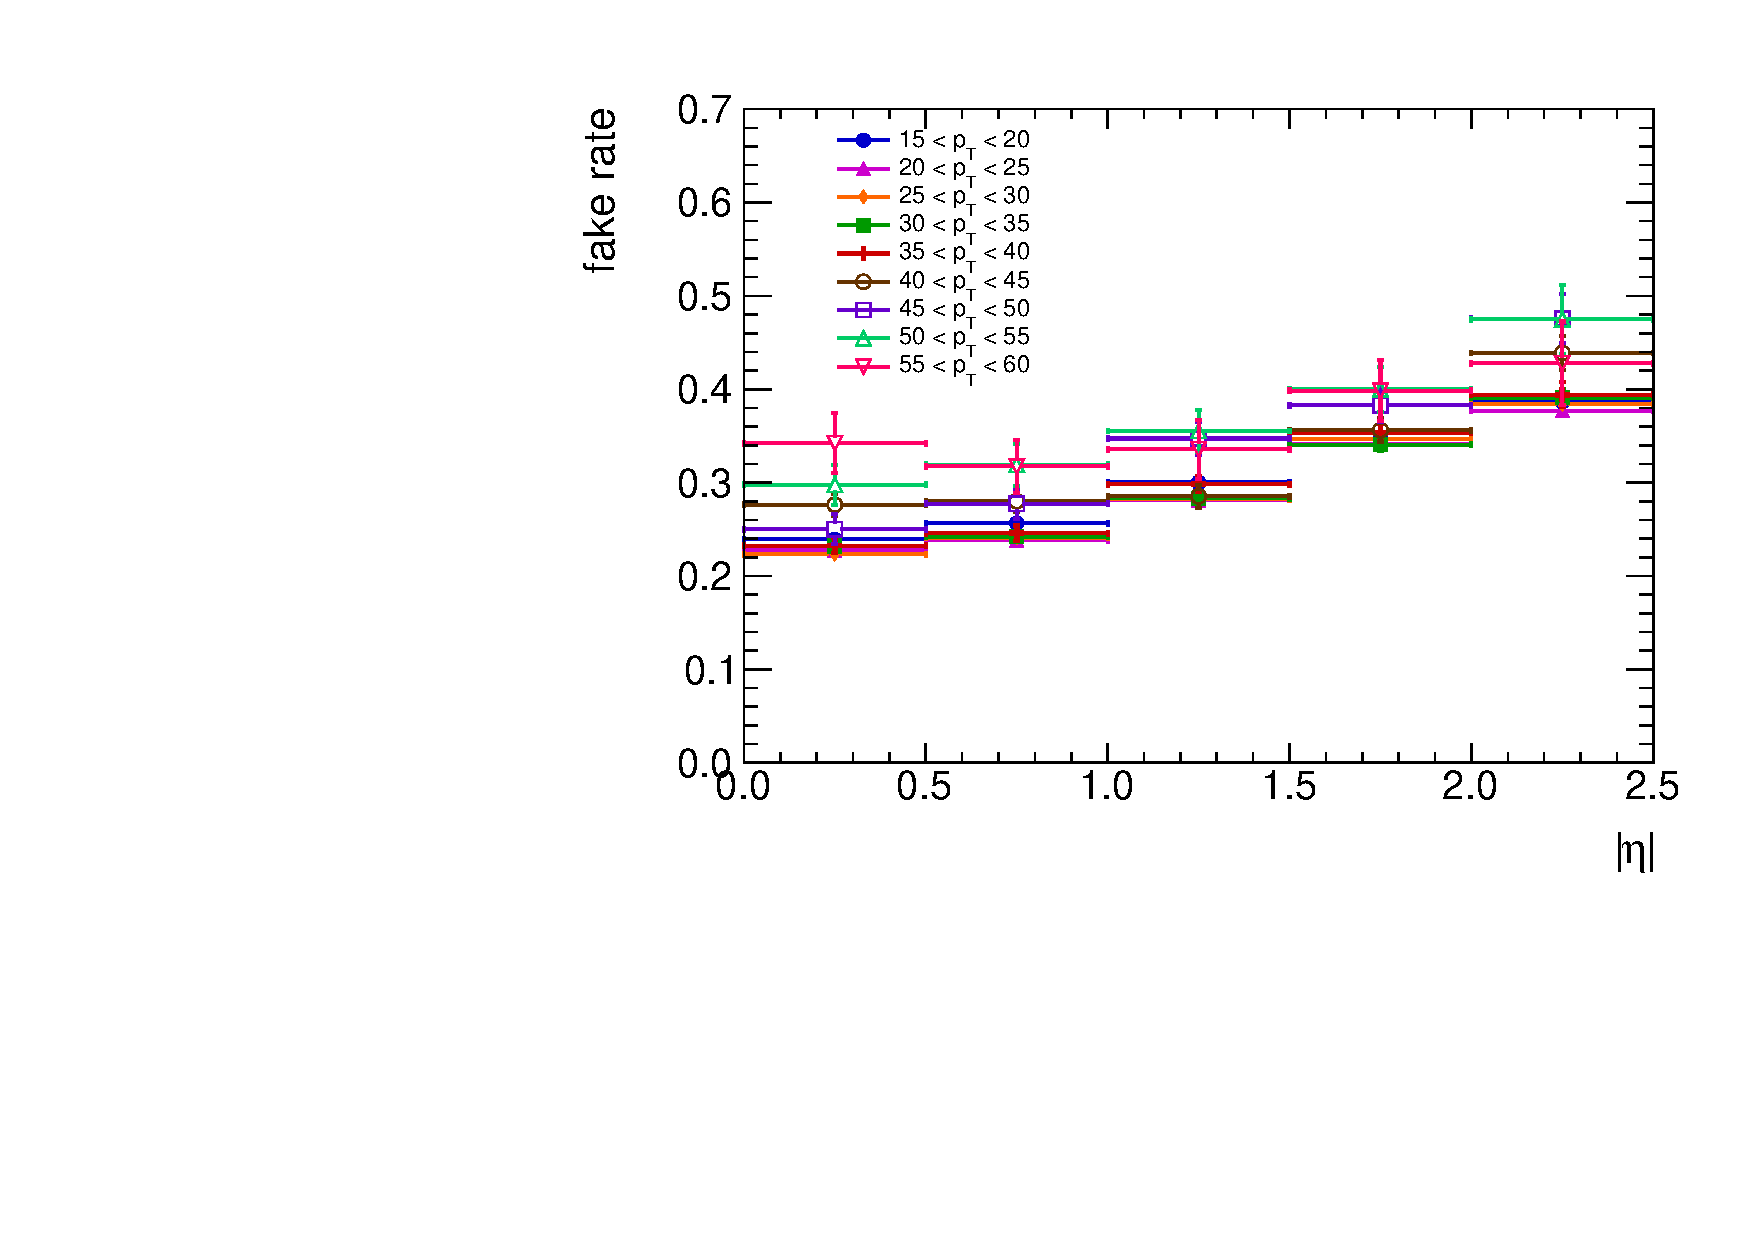
\includegraphics[width=0.45\textwidth]{figs/fakerate_v_eta_m.pdf}}
  \caption{Measured muon fake rates as a function of lepton ~\protect\subref{subfig:fr_vs_pt_e} $\pt$ and ~\protect\subref{subfig:fr_vs_eta_e} $|\eta|$.}
  \label{fig:muon_fr_plots}
\end{center}
\end{figure}

\subsection{Fake rate application}
\label{subsec:fr_app}
The FR does not give a direct measure for an absolute lepton fake rate; it is the probability for a fake lepton which passes loose identification criteria, to additionally pass tight identification and isolation criteria. Thus, to perform the estimate of the fake lepton background, an application sample of ``Tight''$+$``FO'' pairs are obtained by requiring the signal selection with the only modification being that instead of two ``Tight'' leptons, one ``Tight'' lepton and one ``FO'' that fails ``Tight'' selection is required. Each pair is then assigned a weight, FR/$(1-\mbox{FR})$, corresponding to a likelihood that the ``FO'' in the pair will be promoted to a ``Tight'' lepton, and the sum of these weighted pairs give a prediction for the background yield and distributions. In principle, a single event can contribute multiple ``Tight''$+$``FO'' pairs to the application sample, but in practice there is rarely more than one pair from an event.

Dileptonic processes can contaminate the application sample and needs to be subtracted off. MC expectations are used to perform the subtraction; about $95\%$ of this contamination comes from dileptonic $\ttbar$ events.

\subsection{Fake rate closure test}
\label{subsec:fr_close}
As a way to validate the estimation procedure, a closure test is performed in a fakes enriched region. The events in this region are required to pass the same selection as for the signal region, with the modified requirement that the selected leptons must have the same sign. Along with guaranteeing a region enriched in fake leptons, this validation region is also orthogonal to the signal region. A categorization based on \mttll > 110\:\GeV\:is not performed because too few events pass the high \mttll requirement, to make a meaningful test. Good agreement between the data and the combination of simulation and data-driven fake lepton prediction is observed in the \ptmiss distribution, as shown in~\FigureRef{fig:fr_close}. The degree in which the observed and predicted yields disagree is included in the normalization uncertainty on the fakes background prediction in the signal regions.

\begin{figure}
  \begin{center}
    \subfloat[][$ee$ channel]  {\label{subfig:fr_close_ee}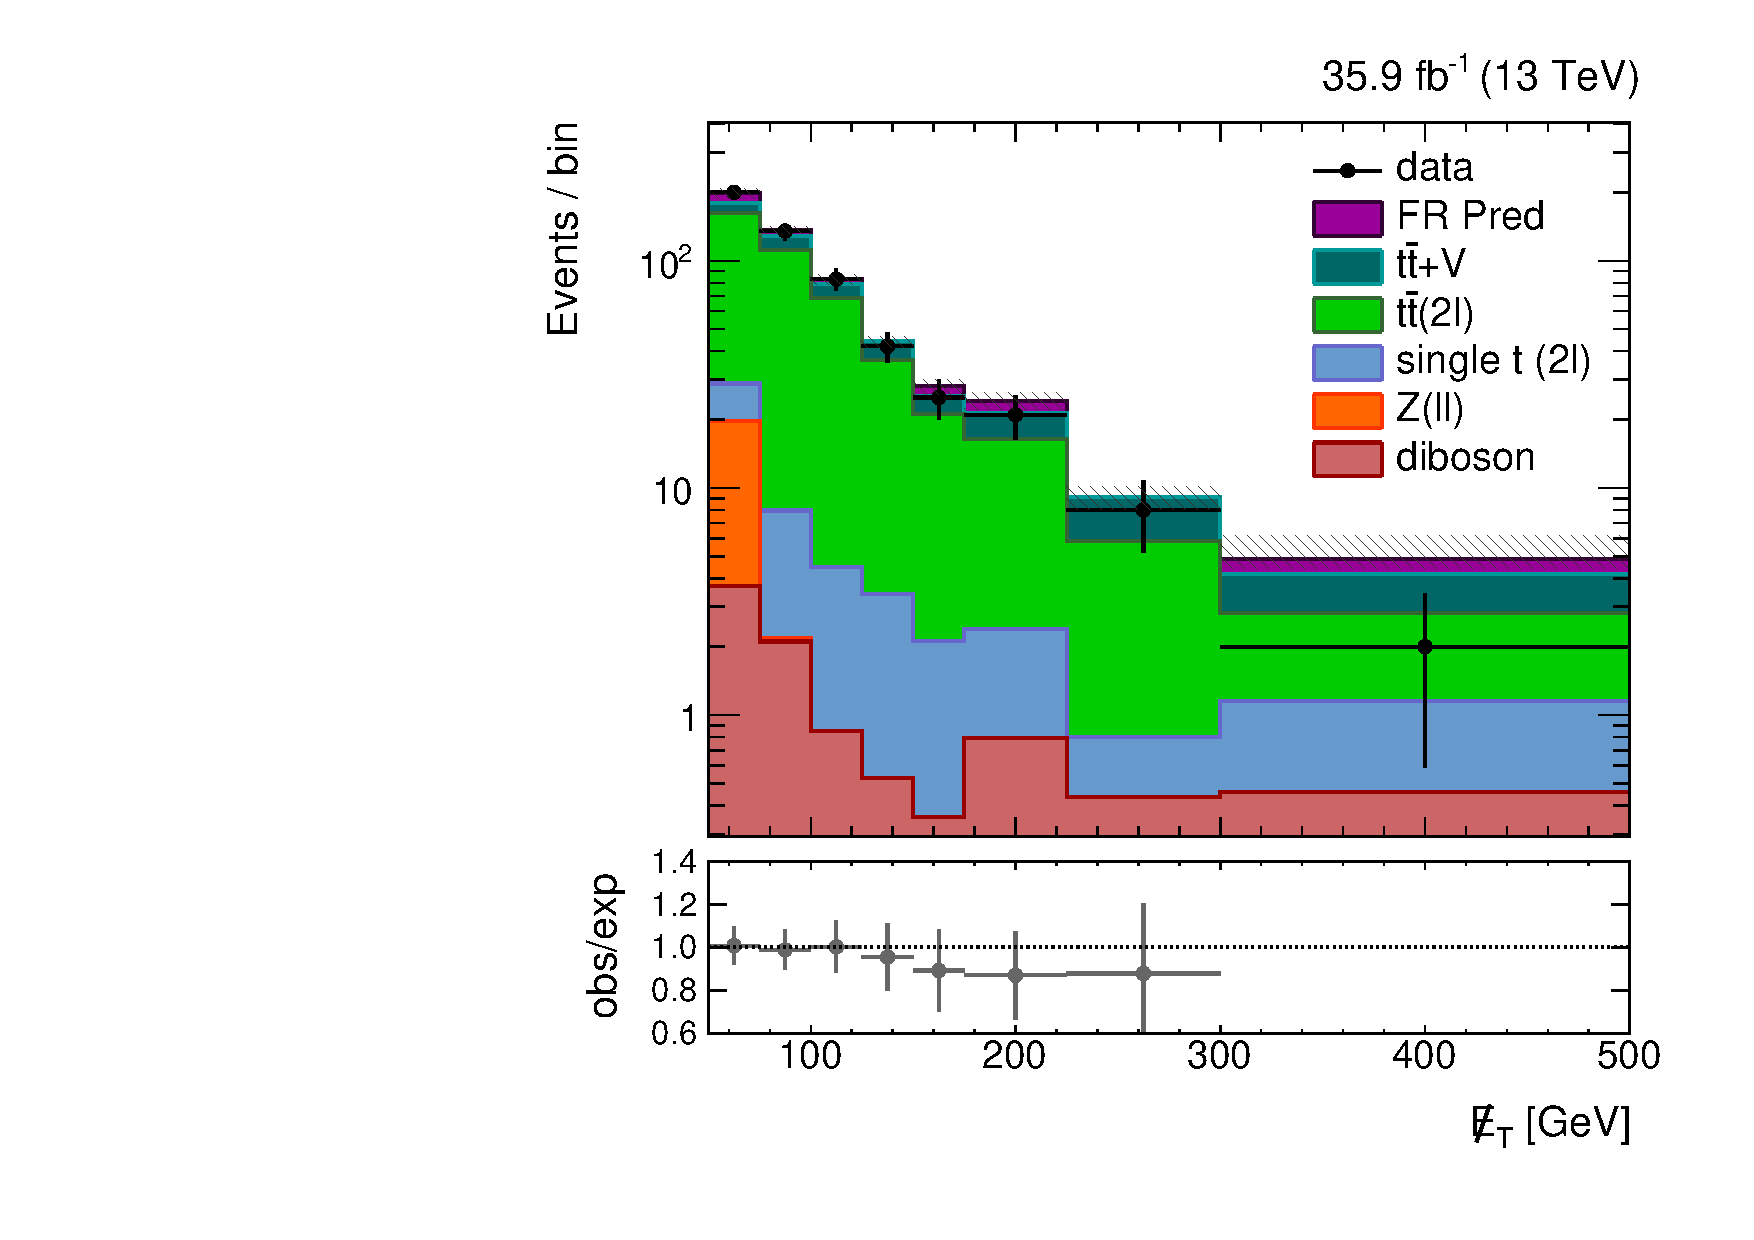
\includegraphics[width=0.32\textwidth]{figs/met_close_ee.pdf}}
  \subfloat[][$e\mu$ channel]  {\label{subfig:fr_close_em}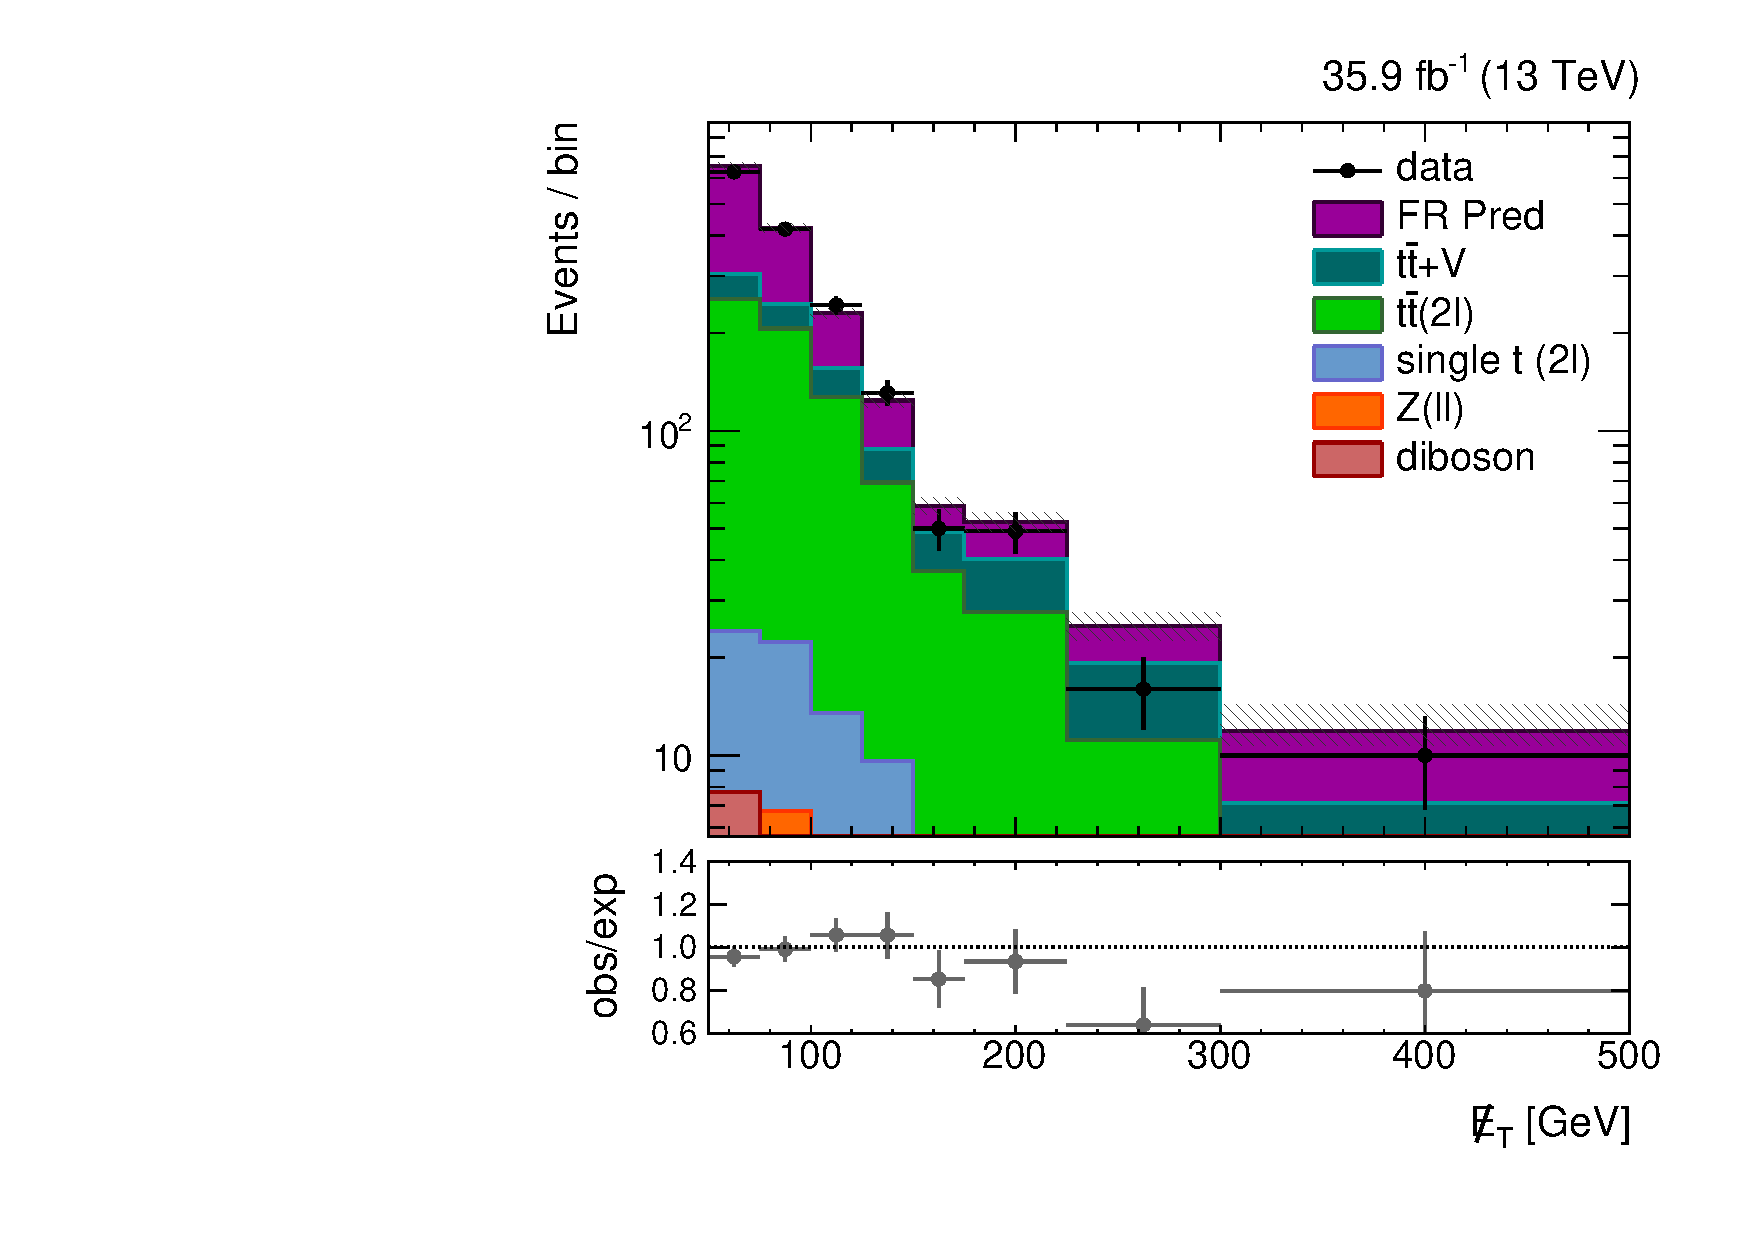
\includegraphics[width=0.32\textwidth]{figs/met_close_em.pdf}}
  \subfloat[][$\mu\mu$ channel]{\label{subfig:fr_close_mm}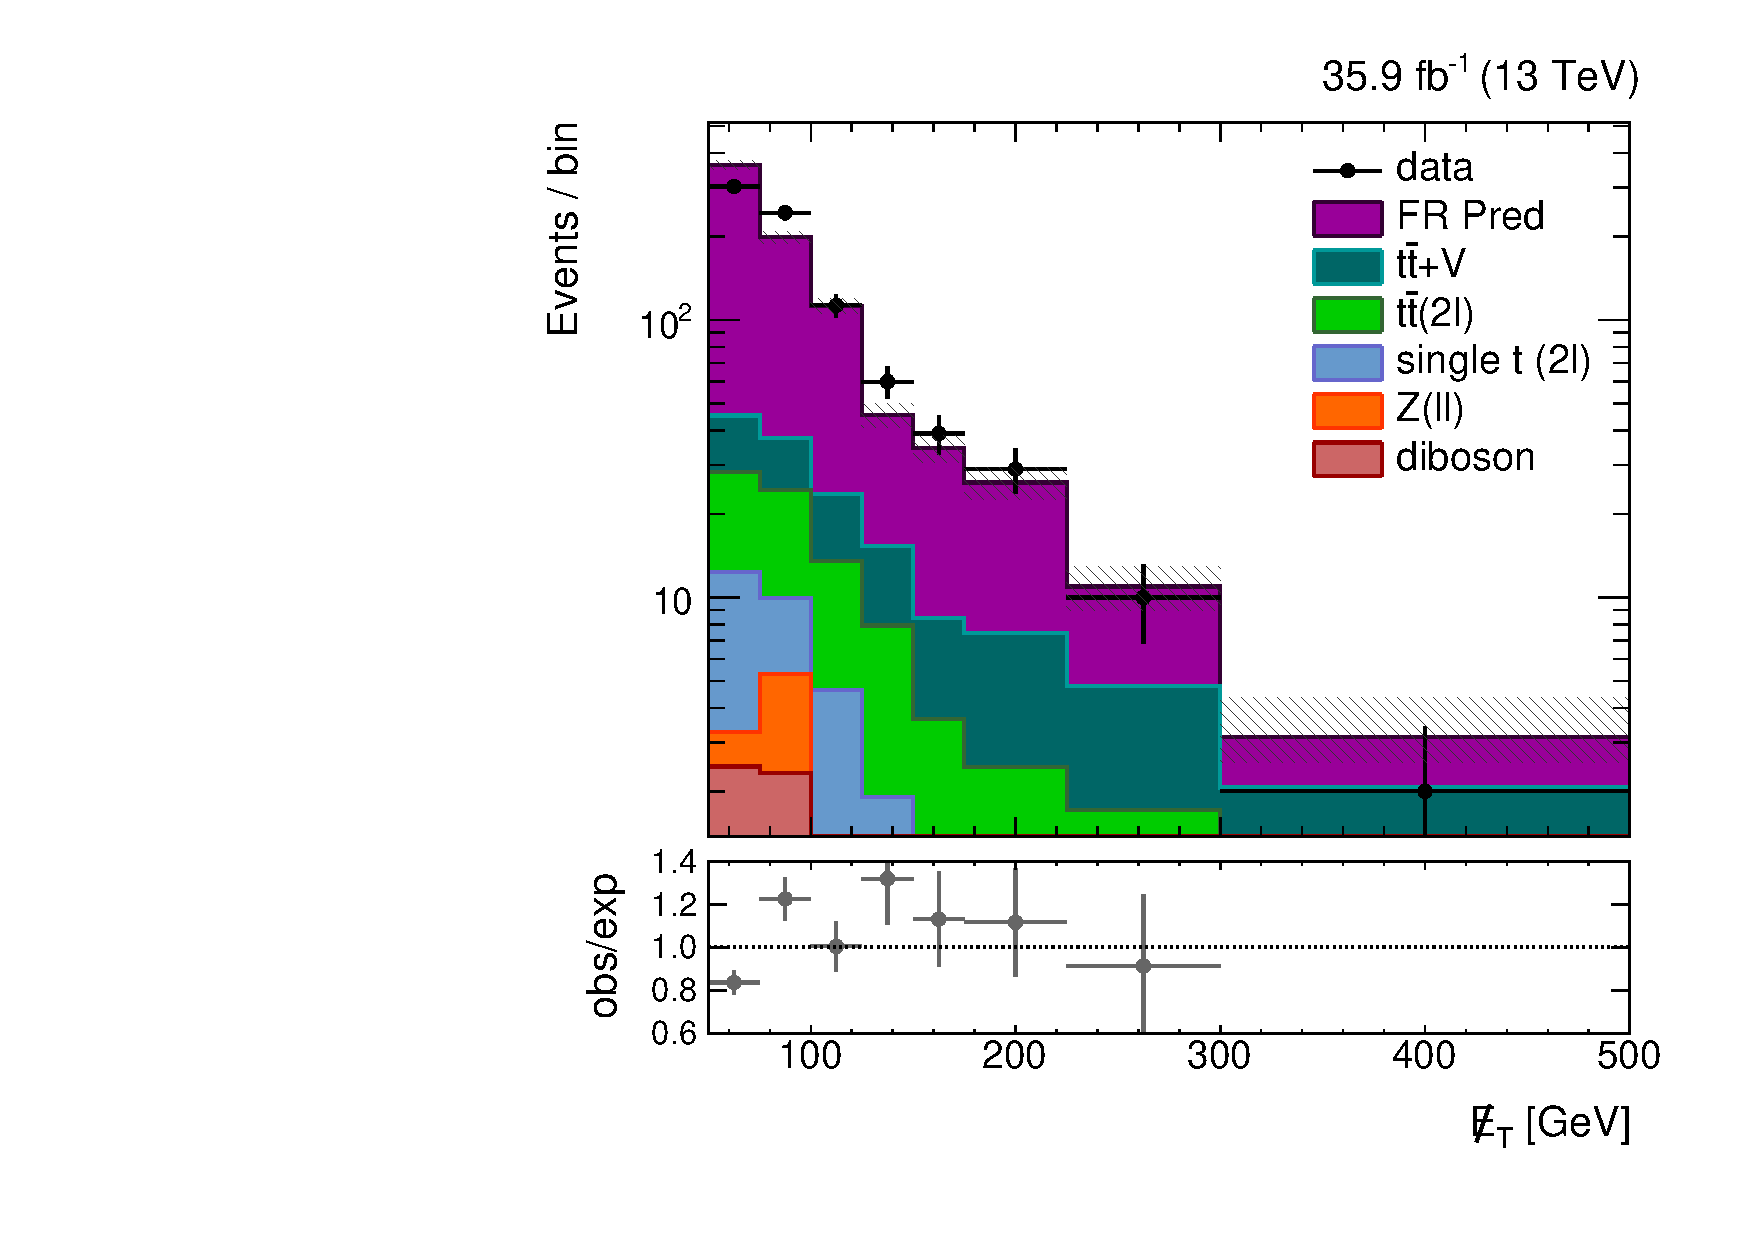
\includegraphics[width=0.32\textwidth]{figs/met_close_mm.pdf}}
  \caption{The \ptmiss distributions in the fake rate method validation region. All expected backgrounds are estimated using simulation, except for the fake lepton contribution, denoted ``FR Pred'' which is estimated via the fake rate method.}
  \label{fig:fr_close}
  \end{center}
\end{figure}

  \chapter{Analysis}
\label{chap:analysis}

\section{Search strategy}
\label{sec:strategy}

The strategy employed in this search is to define regions targeting a high signal acceptance, called signal regions (SRs). As described in Sec.~\ref{sec:selection}, events passing the outlined selection criteria are also categorized according to whether the leptons in the dilepton pair are same or opposite flavor. Additionally, events are divided according to the whether the \mttll quantity is greater or less than 110\:\GeV. Thus, events are split into the following four SRs: high \mttll-SF, high \mttll-OF, low \mttll-SF, and low \mttll-OF. The high \mttll categories are classified as high signal purity regions, whereas the low \mttll categories are dominated by SM \ttll background and thus denoted as low signal purity regions. A potential signal observation would manifest as an excess over the expected \ptmiss from SM background processes, thus the signal extraction strategy is to fit the \ptmiss distribution in the four SRs simultaneously. This approach exploits the kinematic differences between the \ptmiss shapes of the \ttDM signals described in Chap.~\ref{chap:signalsel} and the \ptmiss shapes of SM backgrounds detailed in Chap.~\ref{chap:backgrounds}. The fitting procedure and statistical method is described in Sec.(results/stats chapter). 

\section{Data to simulation corrections}

Various corrections are applied to the simulation to account for mismodeling of distributions in the MC simulation, or to take into account the difference between efficiencies measured in the data compared to those measured in the simulation. The corrections are listed and described below.

\subsection{Trigger efficiency}
\label{subsec:trigger}
\subsection{PU reweighting}
\label{subsec:pu}
The simulation does not predict the PU distribution as observed in the data, so in order to alleviate this discrepancy, the simulation is re-weighted to the estimated PU distribution in data. The re-weighting is derived from the measured instantaneous luminosity of the bunch crossings during the 2016 pp collision data-taking period and the estimated total inelastic cross section. The cross section estimate for 2016 data-taking is 69.2 mb for minimum bias events, with an uncertainty of $4.6\%$. The ratio of normalized distributions of the number of PU interactions in data and \ttll simulation is used to extract the scale factors that are applied to the simulation on an event-by-event basis. The PU profiles in data and simulation are shown in~\FigureRef{fig:pu}, where the simulation is also shown with the minimum bias cross section varied by $\pm4.6\%$ in~\FigureRef{subfig:pileup-unc}. The effect of the PU re-weighting can be seen in~\FigureRef{fig:npv}, where the distribution of the number of reconstructed primary vertices (PV) is shown before and after the re-weighting.

\begin{figure}
  \subfloat[][]{\label{subfig:pileup}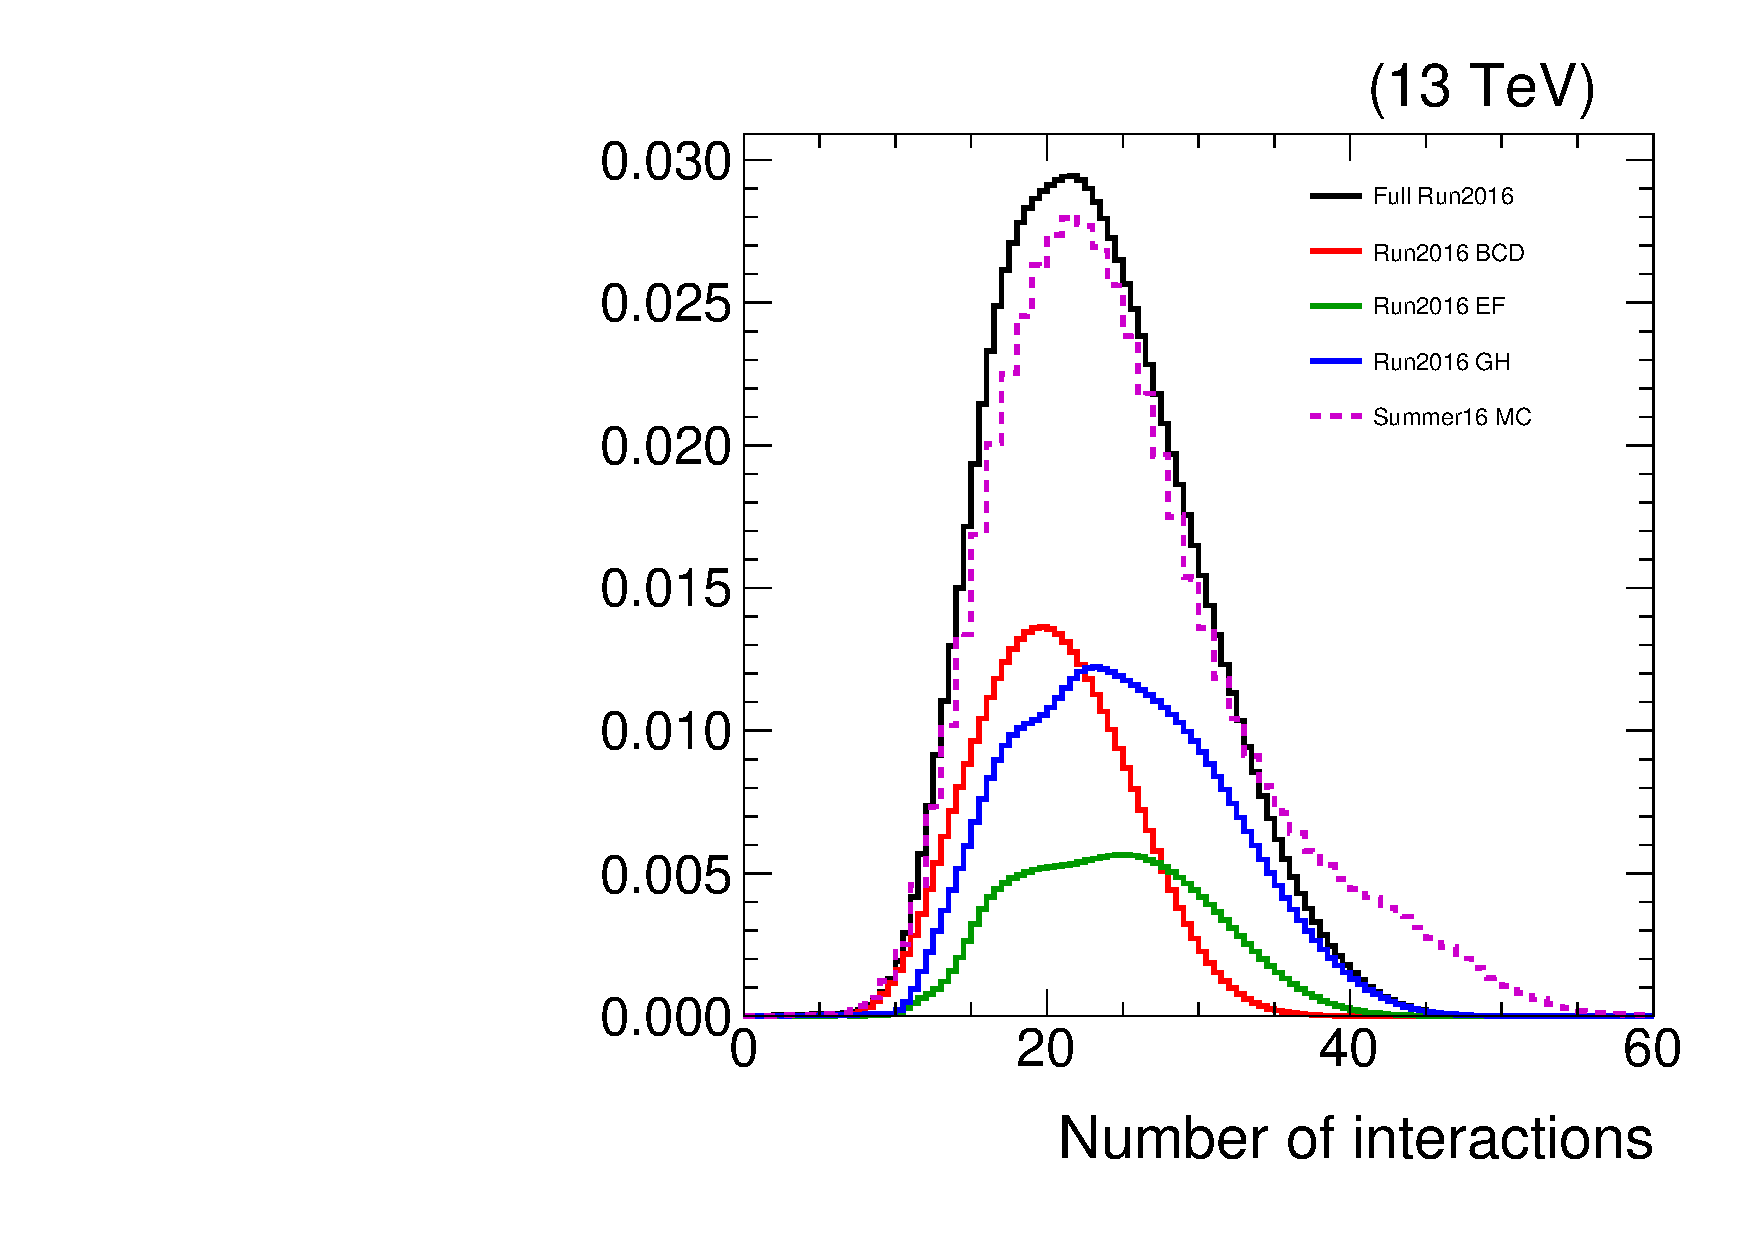
\includegraphics[width=0.48\textwidth]{figs/pileup.pdf}}
  \subfloat[][]{\label{subfig:pileup-unc}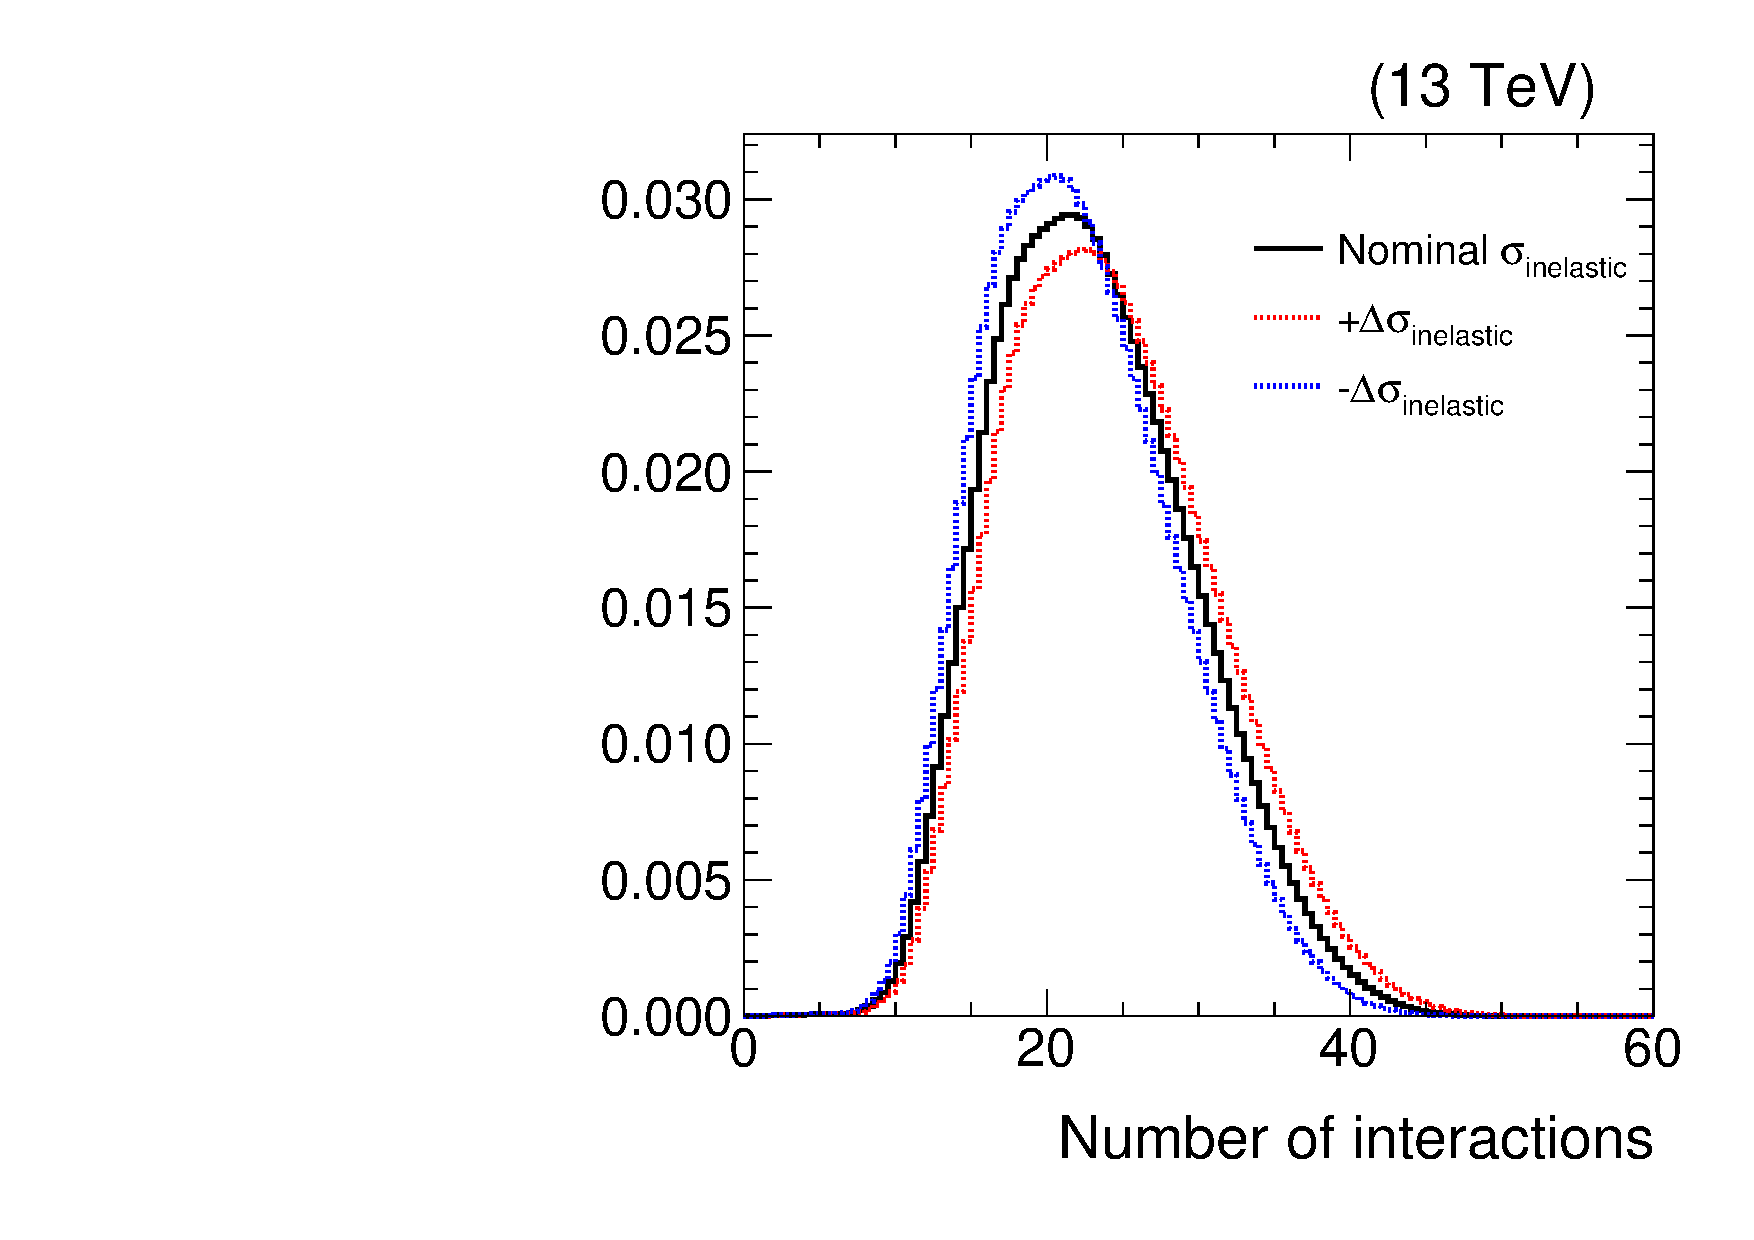
\includegraphics[width=0.48\textwidth]{figs/pileup-unc.pdf}}
  \caption{\protect\subref{subfig:pileup} Pileup distributions in data and MC. Also shown are the pileup profiles in a few run ranges scaled to the relative contribution to the total integrated luminosity.\protect\subref{subfig:pileup-unc} The pileup distributions from varying the total inelastic cross section by $\pm4.6\%$.}
  \label{fig:pu}
\end{figure}

\begin{figure}
%  \subfloat[][]{\label{subfig:npvPRE}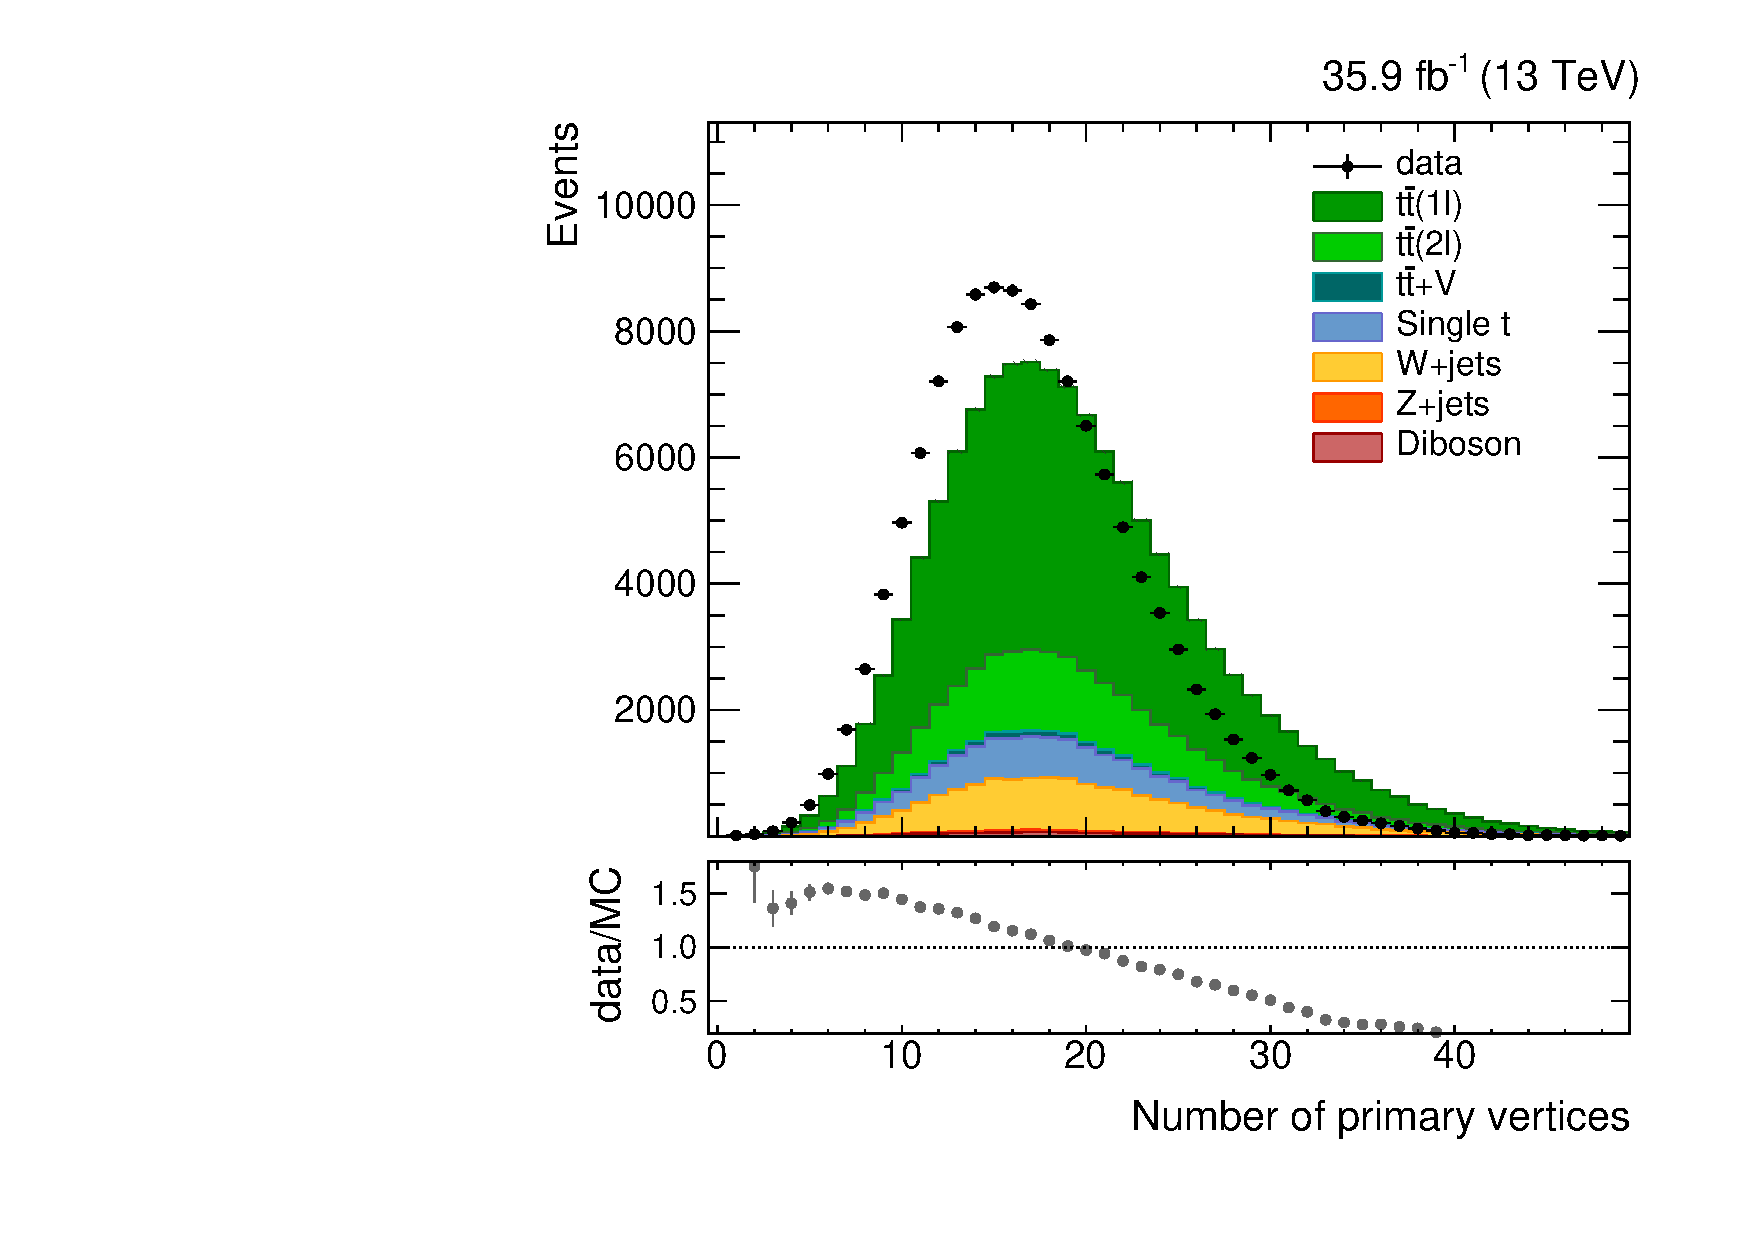
\includegraphics[width=0.48\textwidth]{figs/npv_pre.pdf}}
  \subfloat[][]{\label{subfig:npvPOST}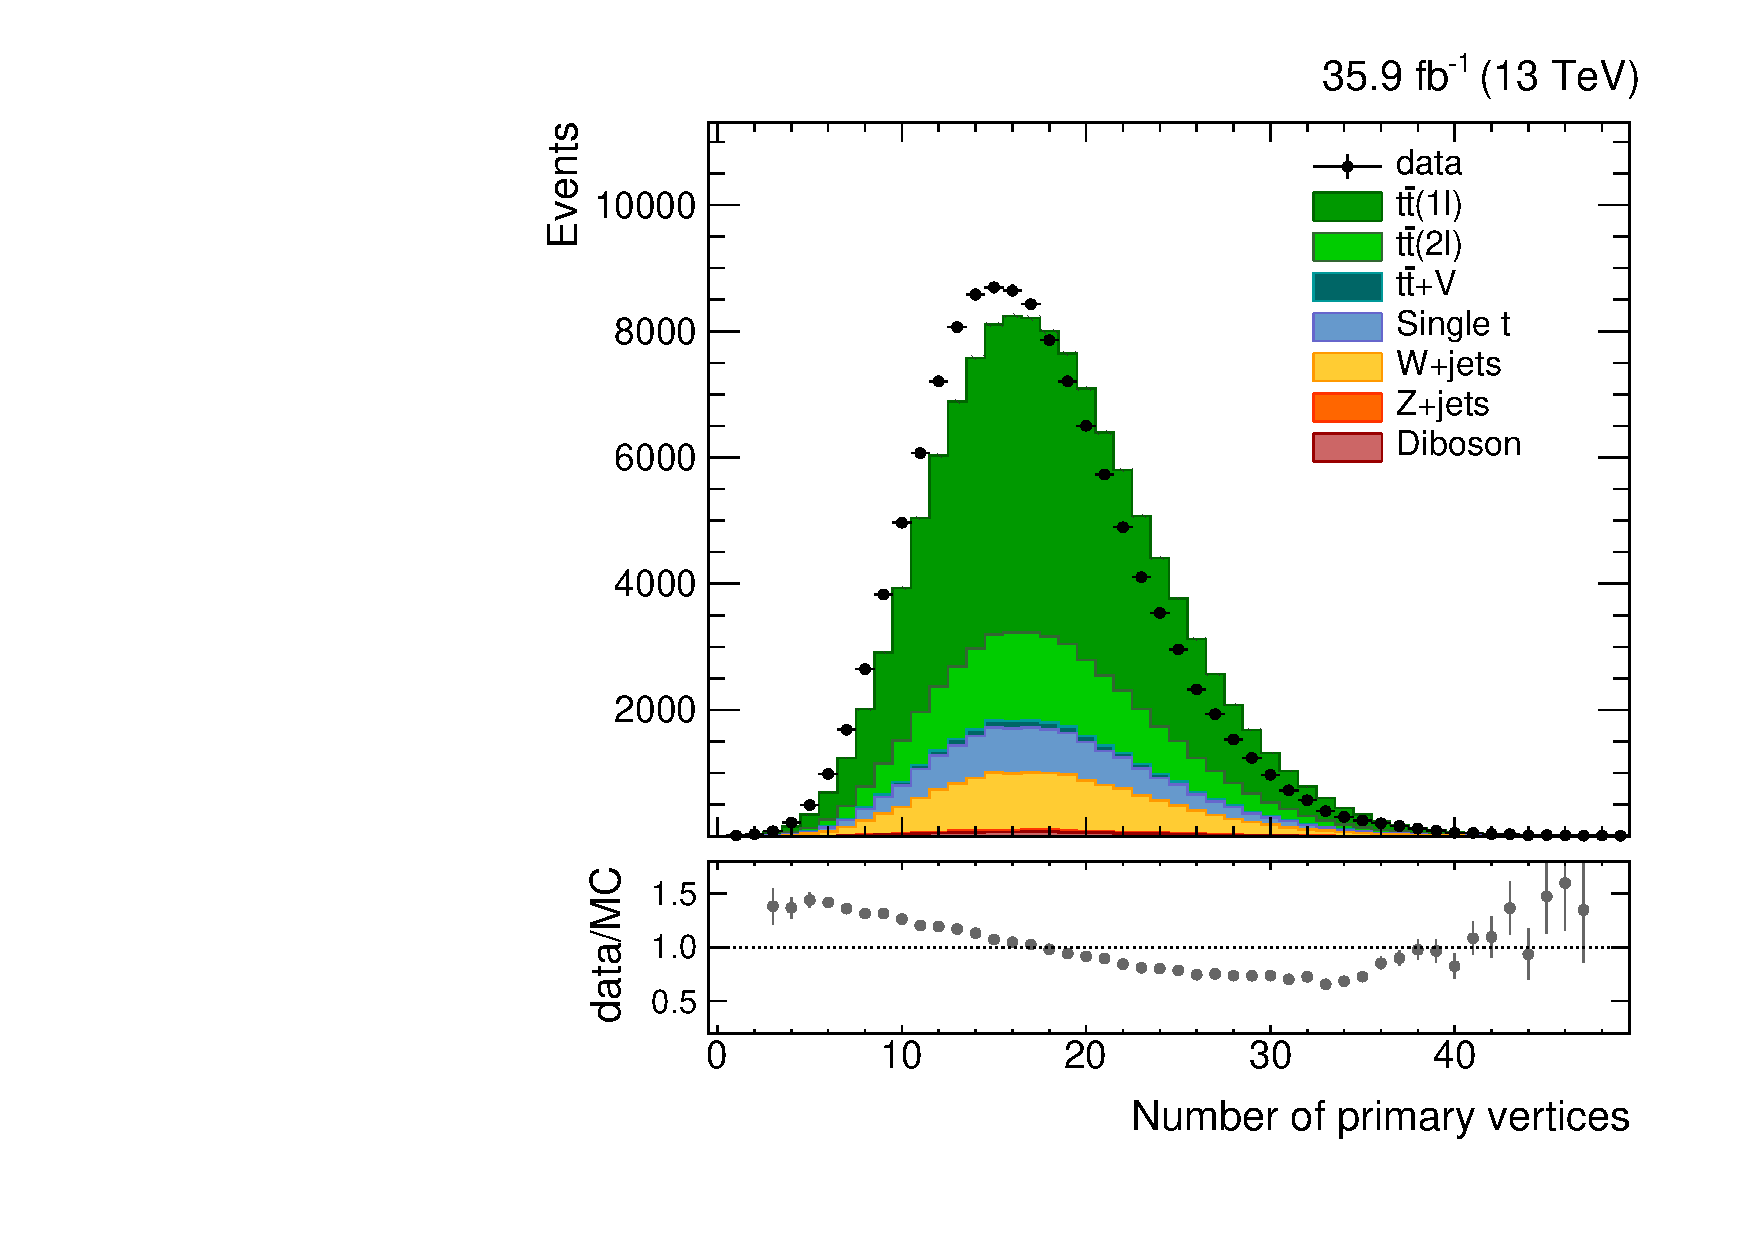
\includegraphics[width=0.48\textwidth]{figs/npv_post.pdf}}
  \caption{$\text{N}_{PV}$ distributions in data and MC pre and post PU re-weighting in a region dominated by semileptonic \ttbar events. The MC is normalized to the observed yield.}
  \label{fig:npv}
\end{figure}
 
\subsection{Top \pt re-weighting}
\label{subsec:toppt}
The generated top quark \pt in \ttbar simulation appears to disagree with the distribution observed in data. The discrepancy arises due to the harder \pt in the simulation as compared to data, thus a correction based on a comparison of the top \pt spectrum between data and the predicted distribution at NLO accuracy from \POWHEG \textsc{v2} interfaced with \Pythia \textsc{v8.2} is used as, developed in ~\cite{Khachatryan:2016mnb}. For each top in a \ttbar MC event, a scale factor is computed according to, 

\begin{equation}
  SF(\pt) = e^{0.0615 - 0.0005\cdot\pt},
  \label{eq:toppt}
\end{equation}

where the exponential function describes the fit to the ratio of data to \POWHEG+\Pythia simulation for dileptonic and semileptonic \ttbar events. The \pt in Eq.~\ref{eq:toppt} is taken at the matrix element level. Subsequently, a weight is applied on an event-by-event basis where the weight is given by the geometric mean of the scale factors,

\begin{equation}
  w = \sqrt{SF(\pt_{t})\cdot SF(\pt_{\bar{t}})}.
\end{equation}

The effect of the re-weighting is seen in~\FigureRef{fig:topPtRwgt} for dilepton signal region events with \mttll< 110\:\GeV\:and \mttll> 110\:\GeV. The correction tends to grow with increasing \ptmiss, since this observable is correlated with top \pt.

\begin{figure}
  \subfloat[][]{\label{subfig:topPt-lo}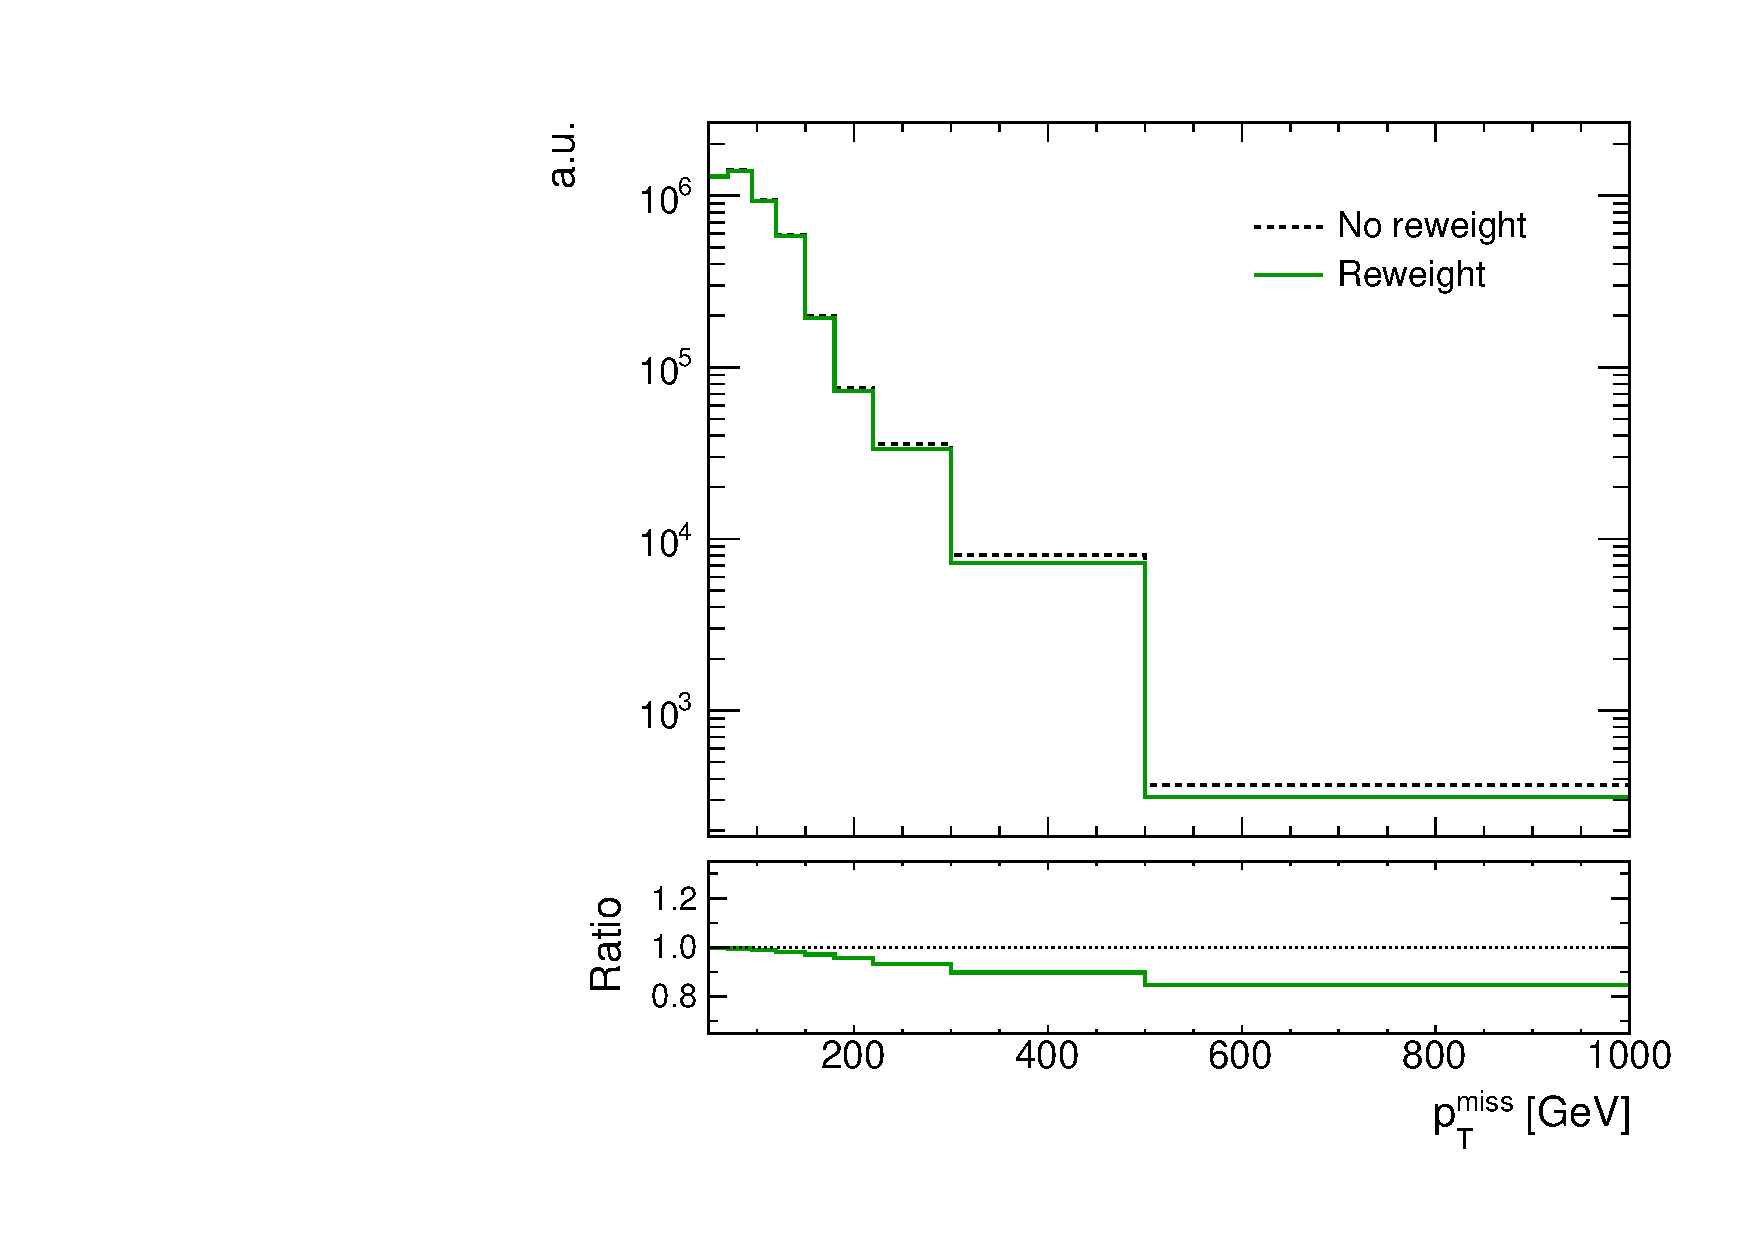
\includegraphics[width=0.48\textwidth]{figs/dilep-lo-ttwgt.pdf}}
  \subfloat[][]{\label{subfig:topPt-hi}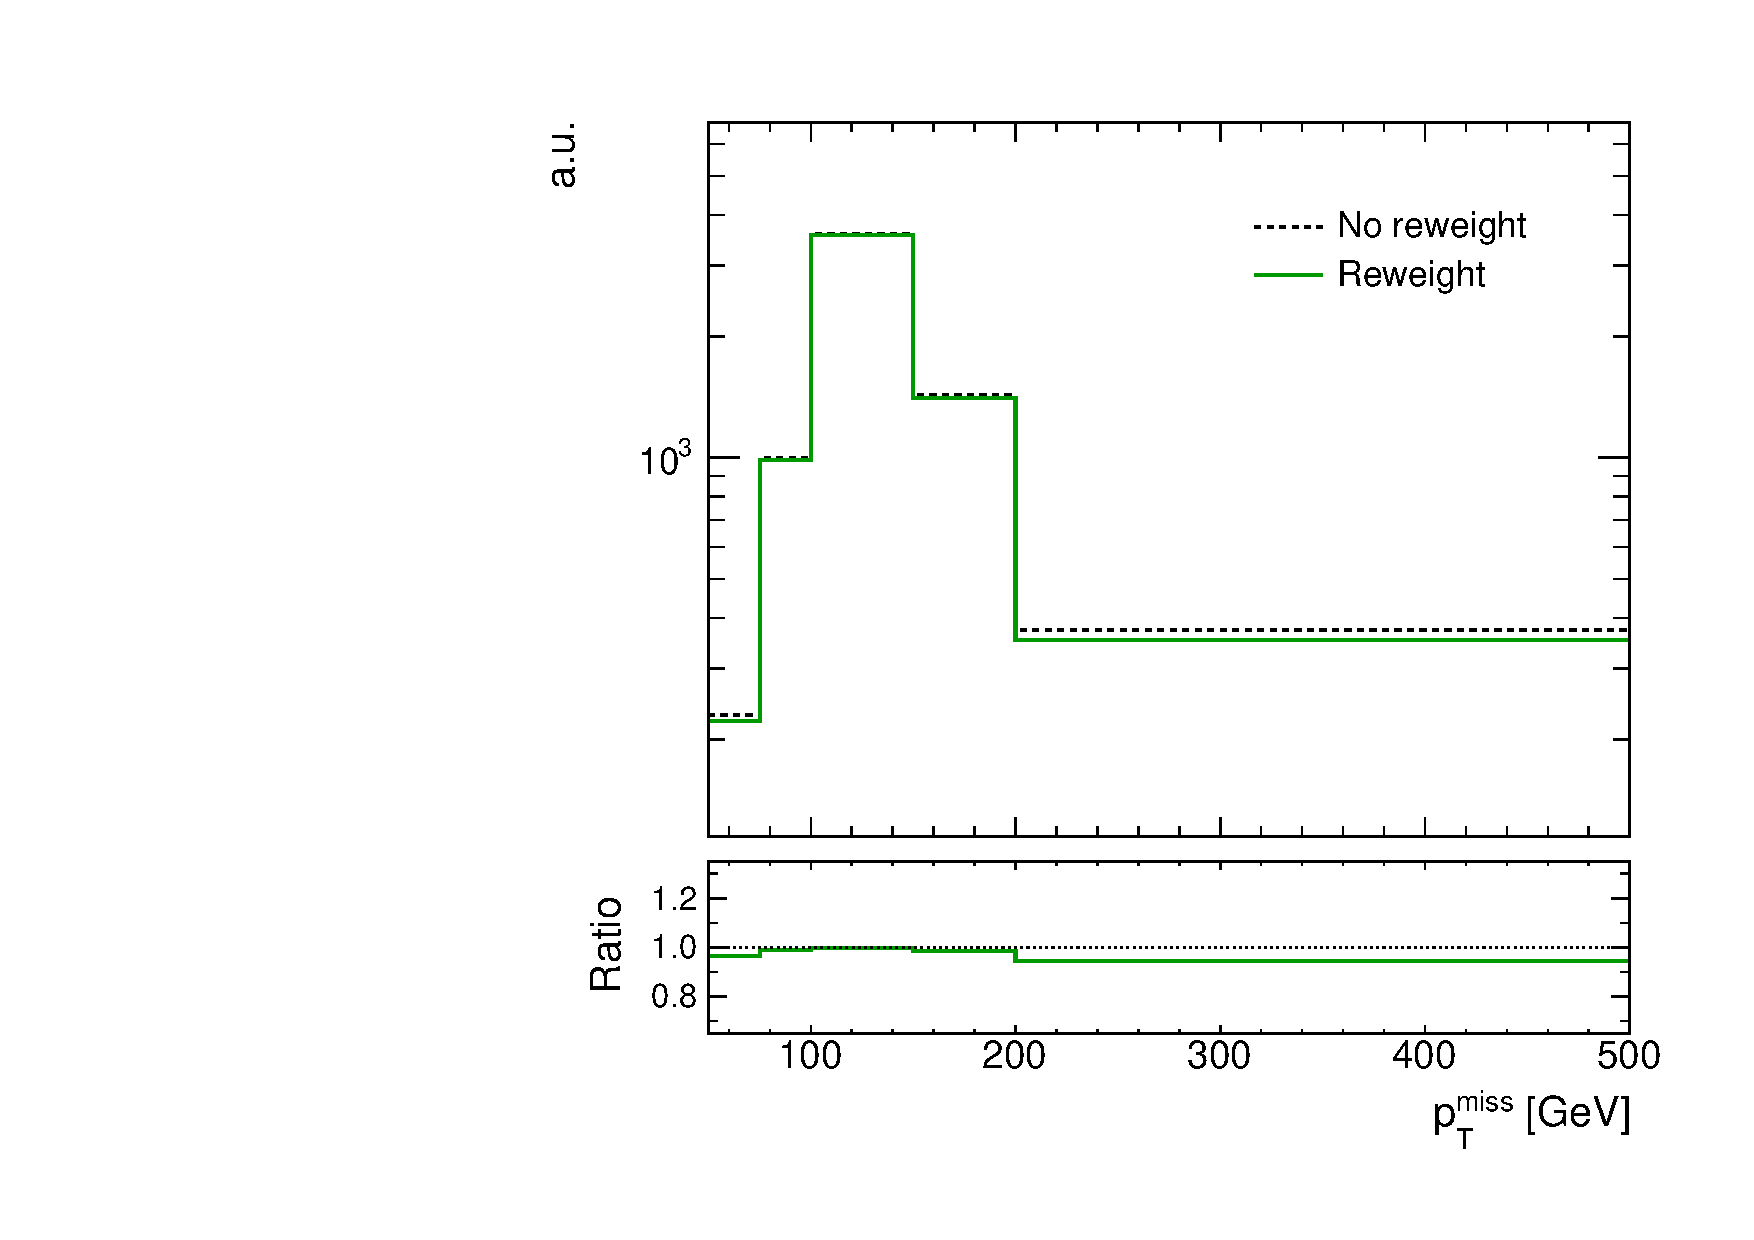
\includegraphics[width=0.48\textwidth]{figs/dilep-hi-ttwgt.pdf}}
  \caption{Effect of the top \pt reweighting on the expected \ttbar background \ptmiss shape for~\protect\subref{subfig:topPt-lo} \mttll < 110\:\GeV\:and~\protect\subref{subfig:topPt-hi} \mttll > 110\:\GeV\:events.}
  \label{fig:topPtRwgt}
\end{figure}

\subsection{b-tagging efficiency}

The efficiency to tag jets orginating from b-quark hadronization is dependent on the working point of the b-tagging algorithm used (in this case the CSV algorithm as defined in Sec.~\ref{subsec:btag}), and the jet kinematics in the signal region of interest. Hence, the performance is characterized based on the probabilities to correctly tag a b jet ($\epsilon_{b}$), to misidentify the hadronization of a c-quark as a b jet ($\epsilon_{c}$), and to misidentify light flavor or gluon initiated jets as b jets ($\epsilon_{udsg}$). Each efficiency is defined by,

\begin{equation}
  \epsilon_{f}(i,j) = \frac{N_{f}^{\text{b-tagged}}(i,j)}{N_{f}^{\text{Total}}(i,j)}, f=b,c,udsg
\end{equation}

where the efficiency is defined in jet \pt bin $i$ and \eta bin $j$, and $N_{f}^{\text{Total}}$ and $N_{f}^{\textrm{b-tagged}}$ are the total number of jets and the number of b-tagged jets of flavor $f$. The efficiency is measured in a simulation sample of dilepton \ttbar and shown in~\FigureRef{fig:btageff} for each jet flavor as a funtion of \pt and \eta.

\begin{figure}
  \subfloat[][]{\label{subfig:beff}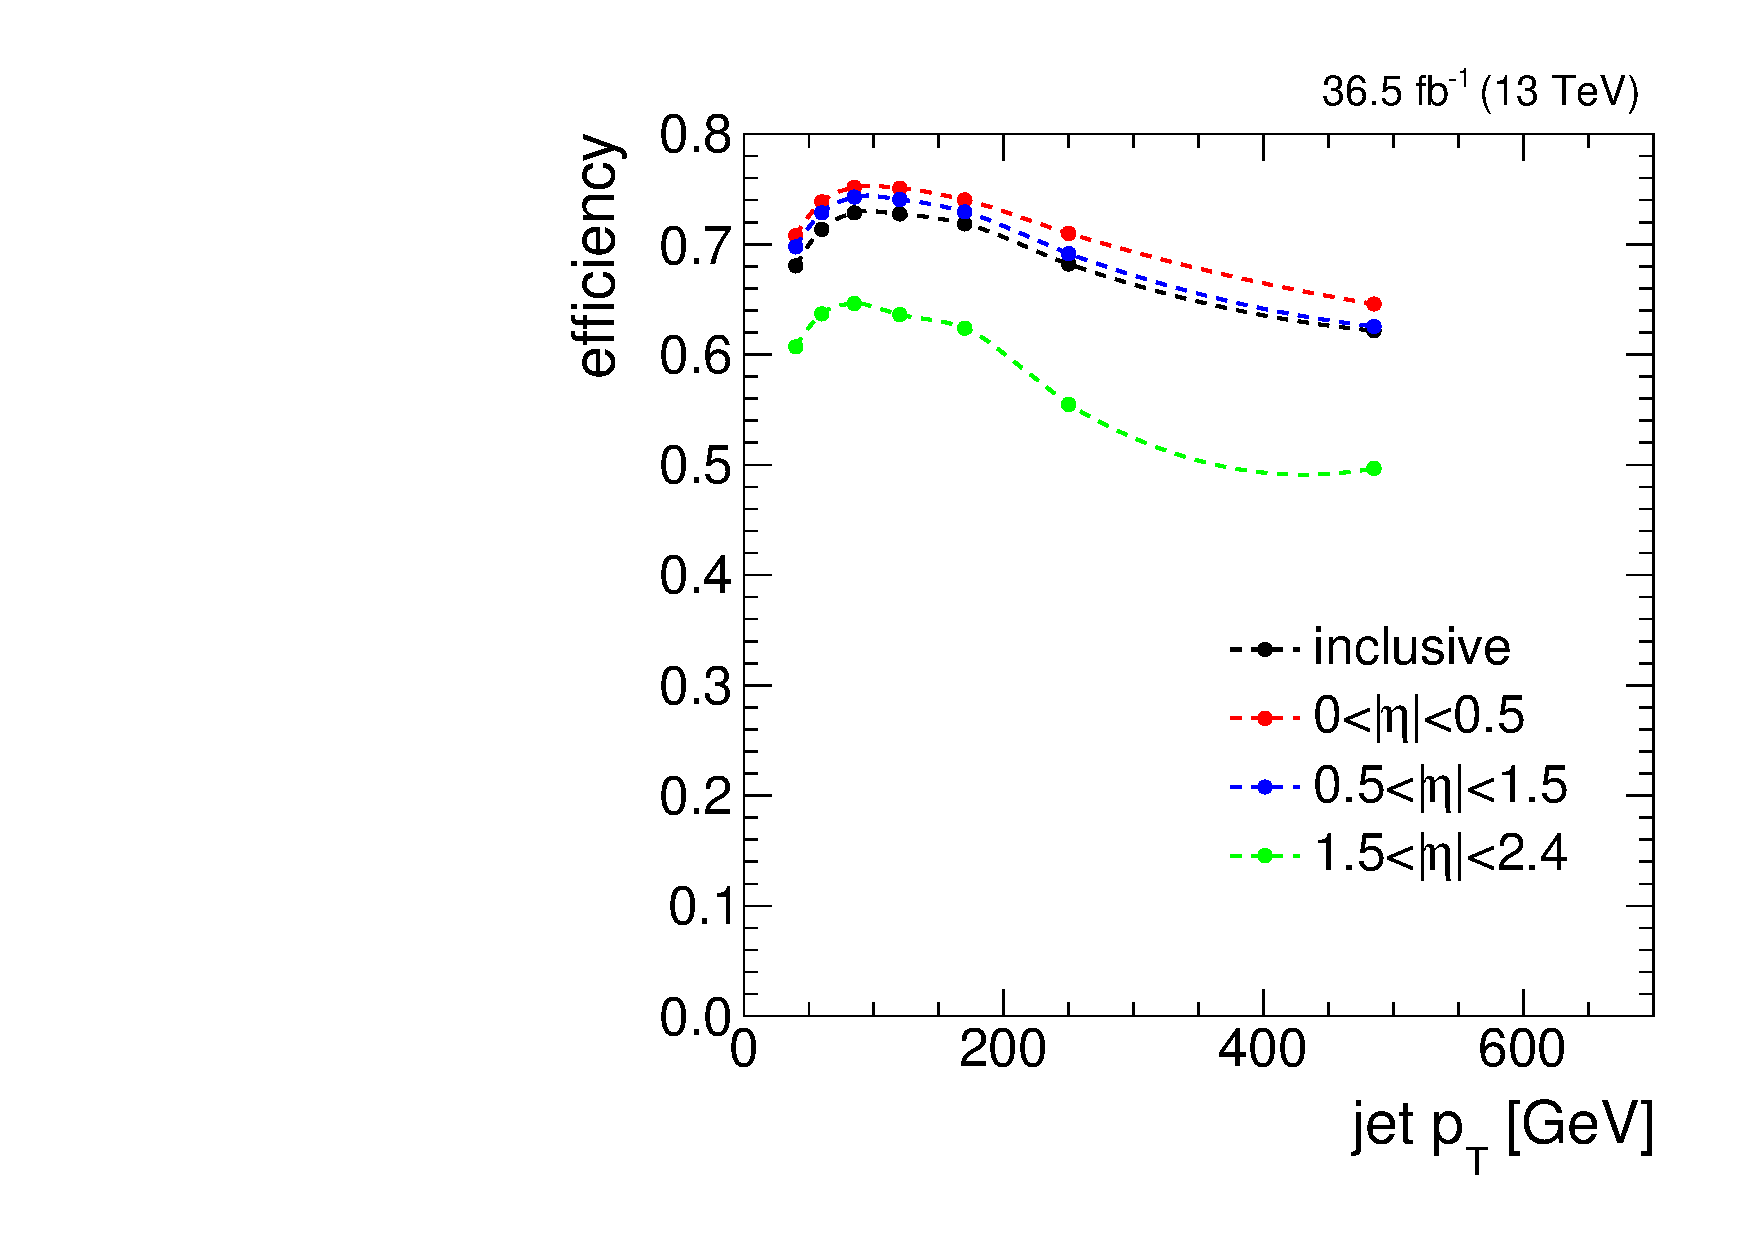
\includegraphics[width=0.48\textwidth]{figs/b_effpt.pdf}}
  \subfloat[][]{\label{subfig:ceff}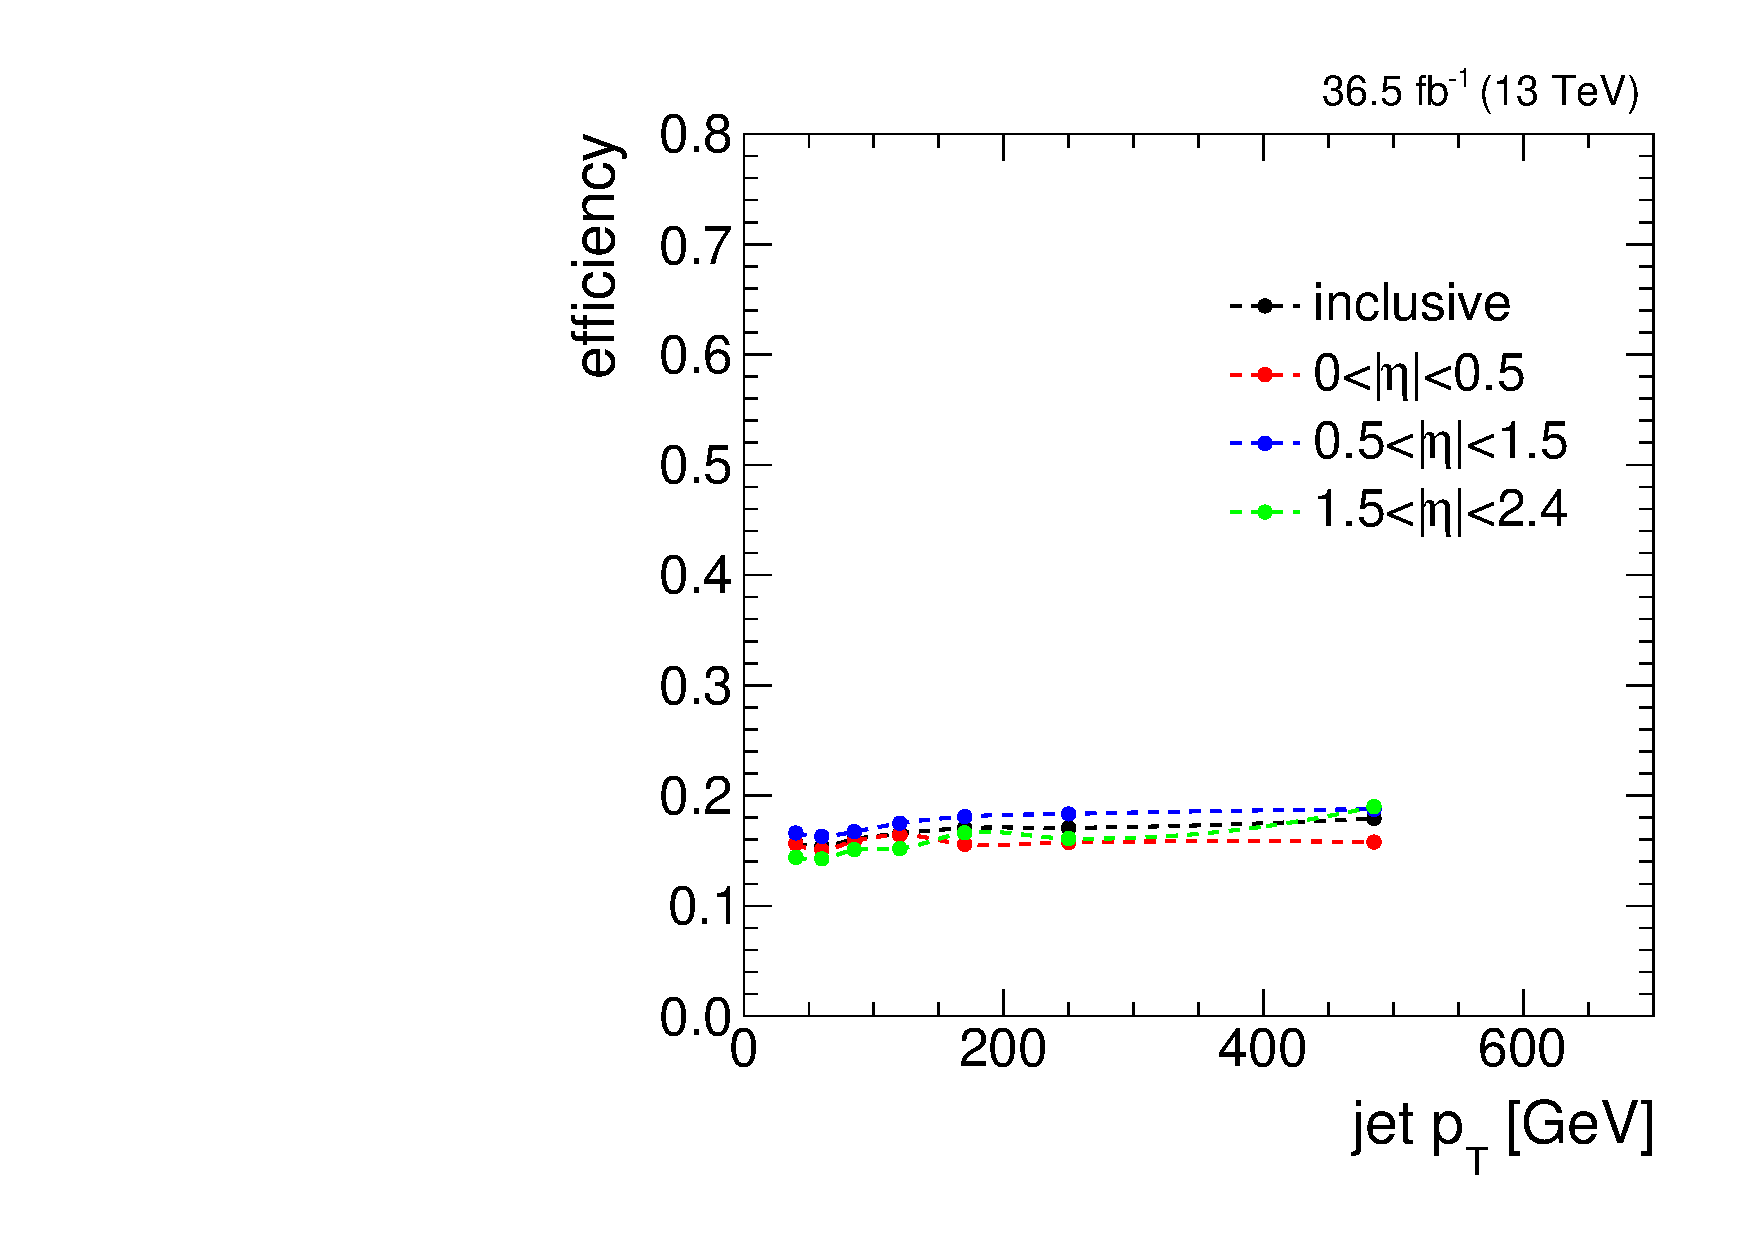
\includegraphics[width=0.48\textwidth]{figs/c_effpt.pdf}}\\
  \subfloat[][]{\label{subfig:leff}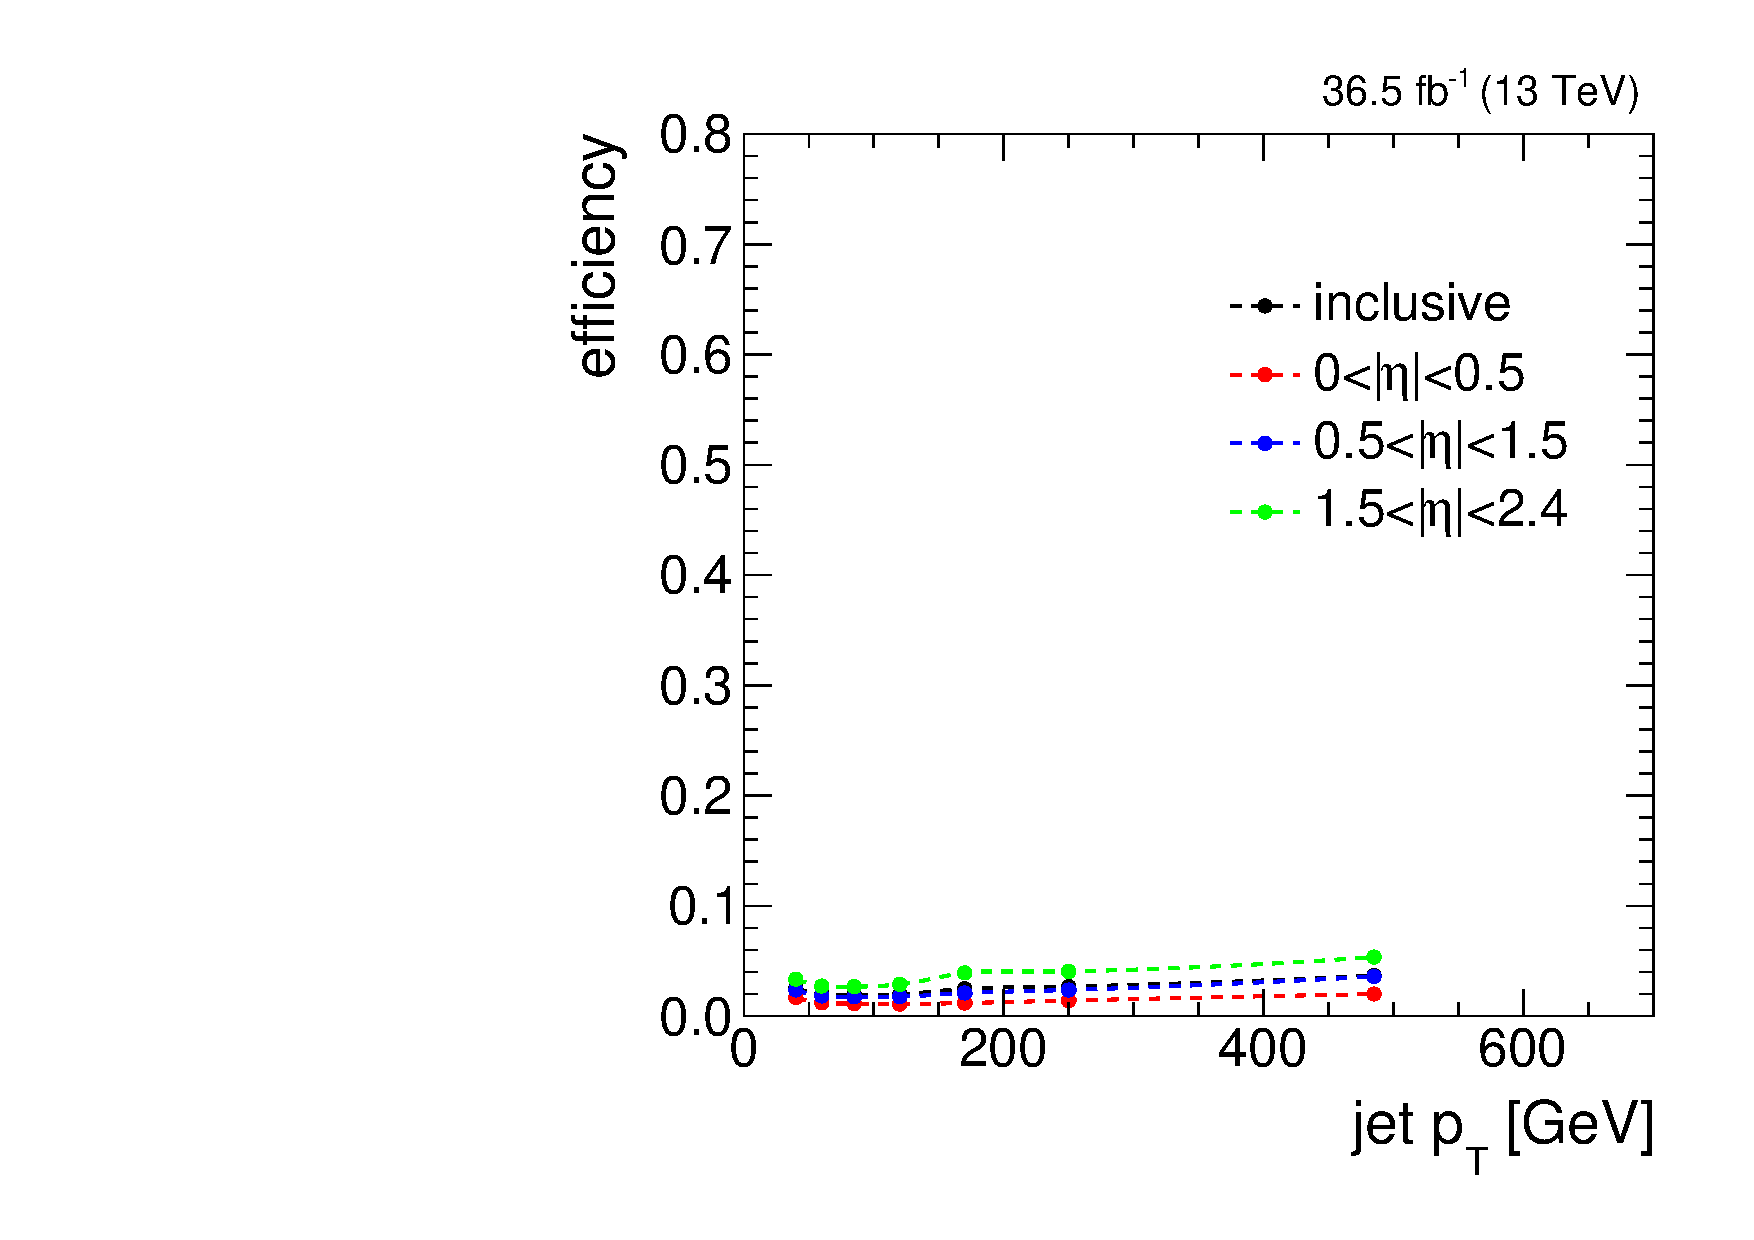
\includegraphics[width=0.48\textwidth]{figs/l_effpt.pdf}}
  \caption{The efficiency measured as a function of jet \pt and various \eta bins for~\protect\subref{subfig:beff} correctly tagging b jets,~\protect\subref{subfig:ceff} misidentifying c jets,~\protect\subref{subfig:leff} and misidentifying light flavor or gluon jets.}
  \label{fig:btageff}
\end{figure}

The CSV algorithm has three working points which correspond to different values of $\epsilon_{udsg}$ as measured in data. They are defined as loose ($\epsilon_{udsg}=~10\%$), medium ($\epsilon_{udsg}=~1\%$), and tight ($\epsilon_{udsg}=~0.1\%$). In the following analysis, the medium working point is used and corresponds to a b-tagging efficiency of $\epsilon_{b}=69\%$, and an c-jet mistag efficiency of $\epsilon_{c}=35\%$ in data. The corrections are applied to the simulation based on the ratio of efficiencies measured in the data and simulation, in order to cover any differences in efficiency with respect to the performance in data.

\section{Discriminating observables}
\label{sec:observables}

\ptmiss is the detector observable which provides the strongest discrimination between the \ttDM signal and the dominant SM dileptonic \ttbar background. In addition to the main observable used for the signal extraction, multiple other observables are scrutinized as a means to check the background modeling and ascertain if discrepancies between the data and the simulation exist in the signal region. These can be seen in the same flavor and opposite flavor channels, respectively, in ~\FigureRef{fig:dilep_sr_sf} and ~\FigureRef{fig:dilep_sr_em}. The observables include the multiplicity of jets ($N_{\textrm{jets}}$), and that of b-tagged jets ($N_{\textrm{b-jets}}$), as well as kinematic distributions for the highest \pt (leading) lepton and jet in the event. The 4-vectors of the two leptons in the event are summed to obtain the \pt and mass of the dilepton system, $\pt^{\ell\ell}$ and $m_{\ell\ell}$. The azimuthal separation between the dilepton system and the \ptvecmiss, $\Delta\phi(\ell\ell,\ptvecmiss)$, is also shown, along with the uncategorized \ptmiss spectrum.

The \mttll distribution used to categorize events into a low ($\mttll<110\:\GeV$) and high ($\mttll>110\:\GeV$) signal purity category is shown in ~\FigureRef{fig:mt2_sr}. The subsequent \ptmiss spectra in the low and high purity signal regions are shown in ~\FigureRef{fig:metlo} and ~\FigureRef{fig:methi}, respectively. 


\begin{figure}[h!]
  \centering
  \subfloat[$N_{\textrm{jets}}$]   {\label{subfig:njets_sf}    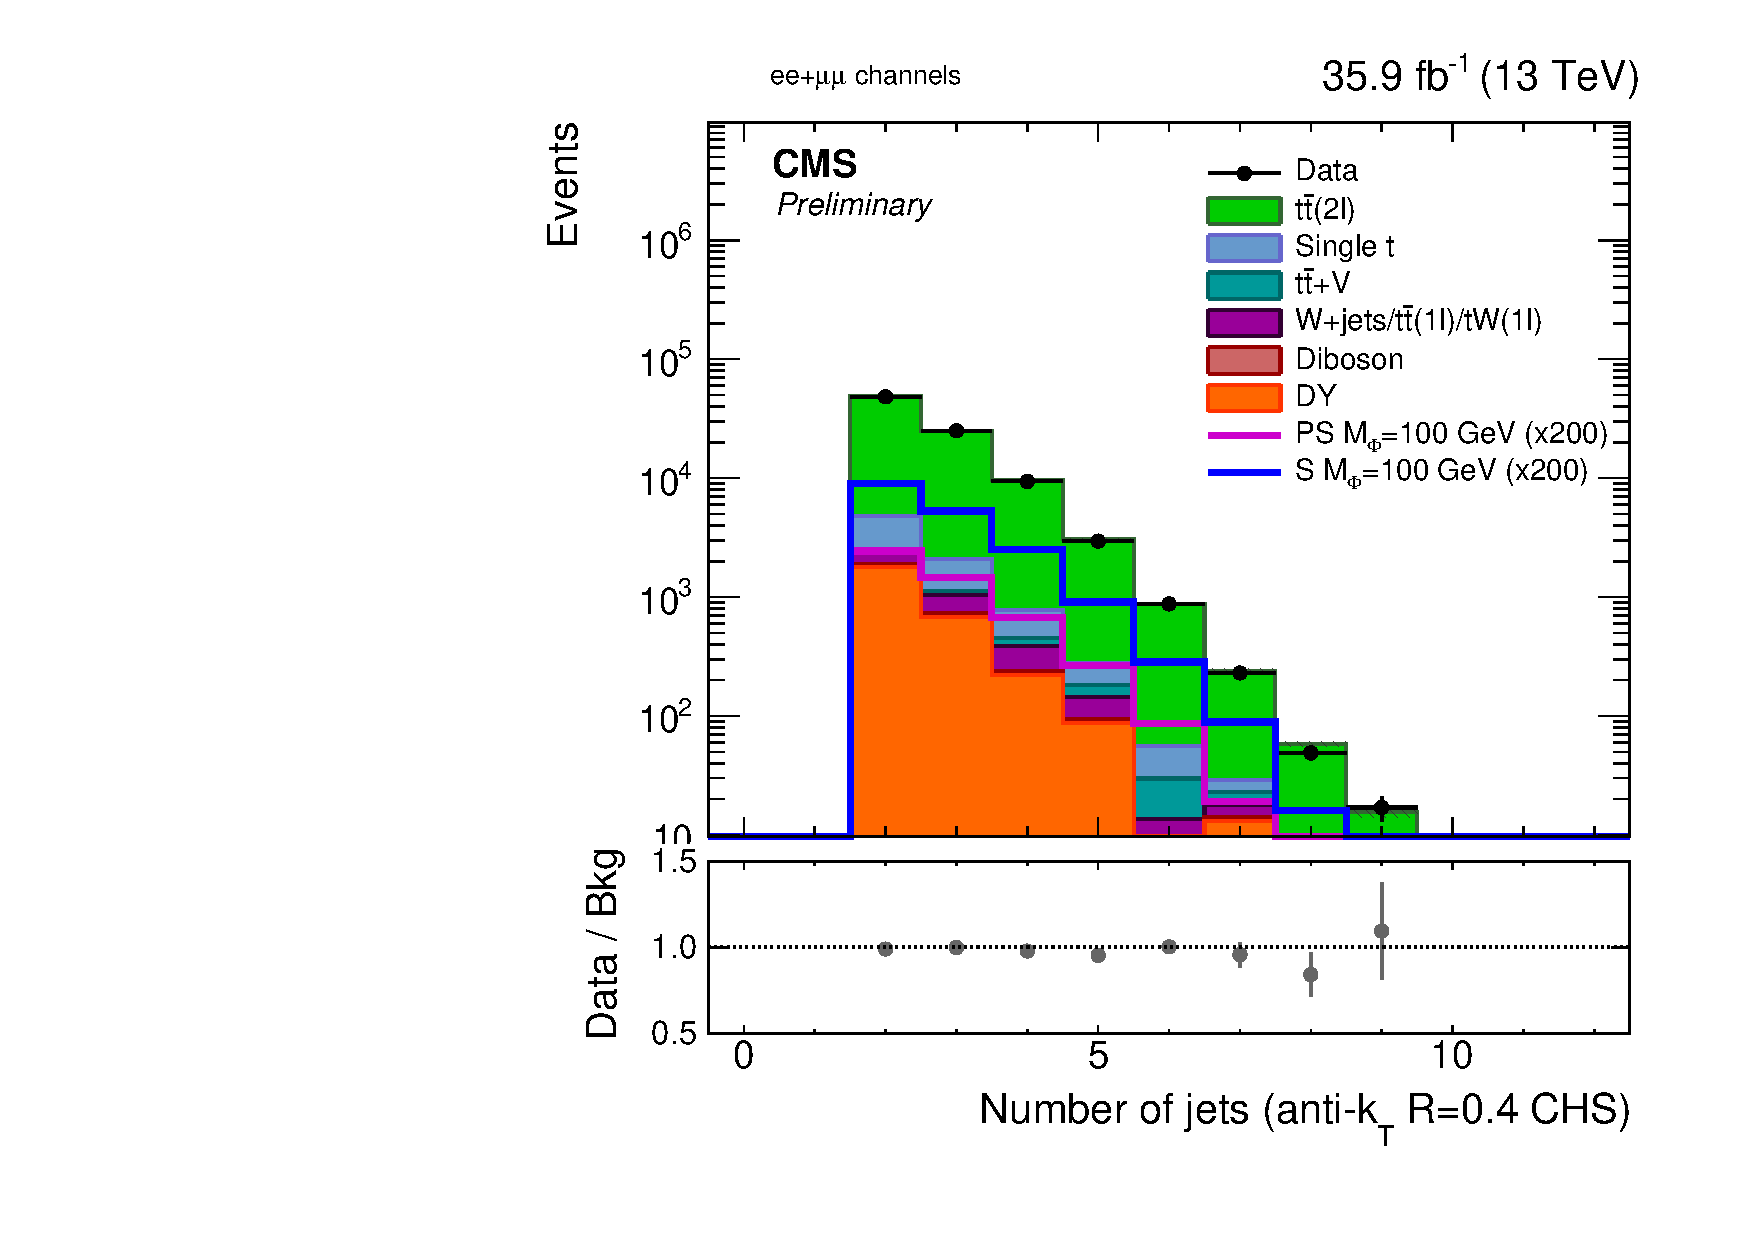
\includegraphics[width=0.43\textwidth]{figs/inclusiveSR/njets_sf.pdf}}
  \subfloat[$N_{\textrm{b-jets}}$] {\label{subfig:nbjets_sf}   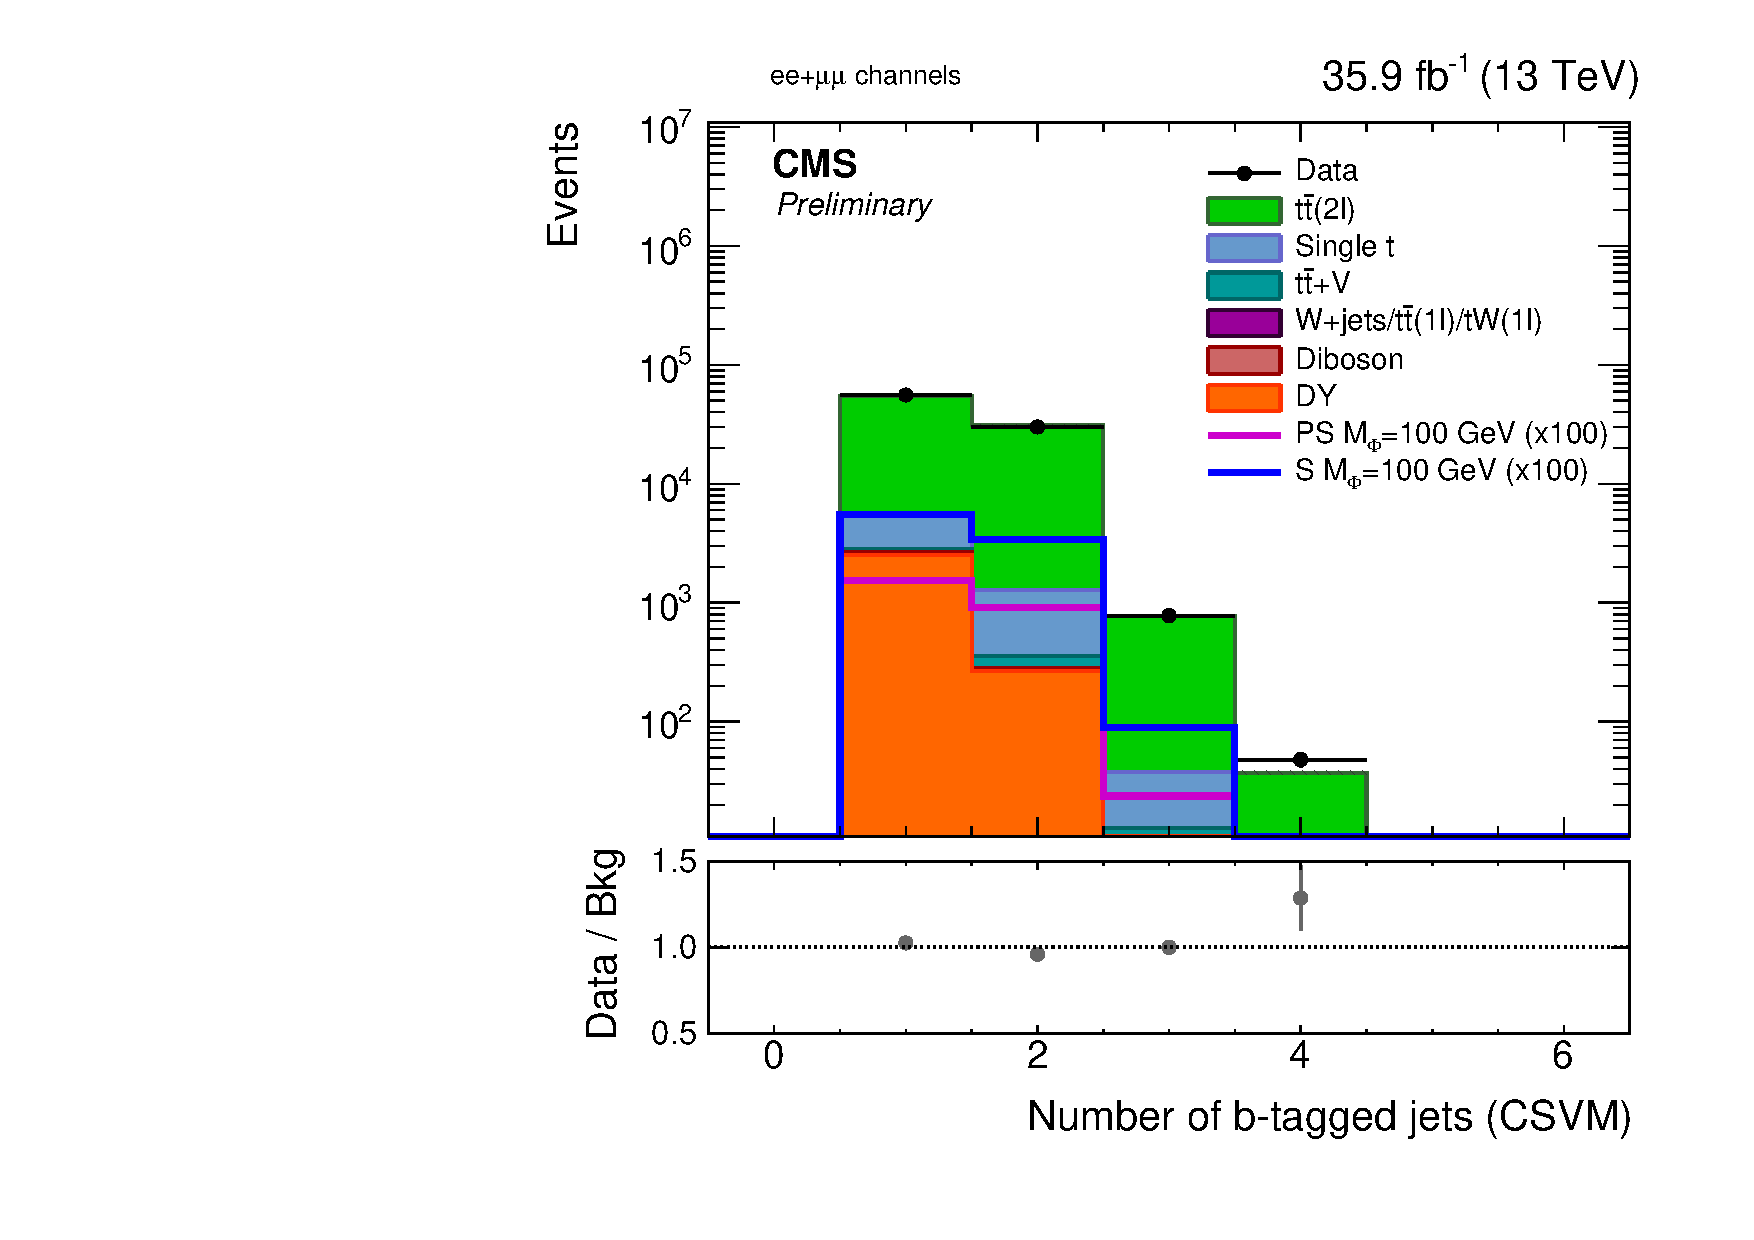
\includegraphics[width=0.43\textwidth]{figs/inclusiveSR/nbjetsm_sf.pdf}} \\
  \subfloat[leading lepton $\pt$]  {\label{subfig:leppt_sf}    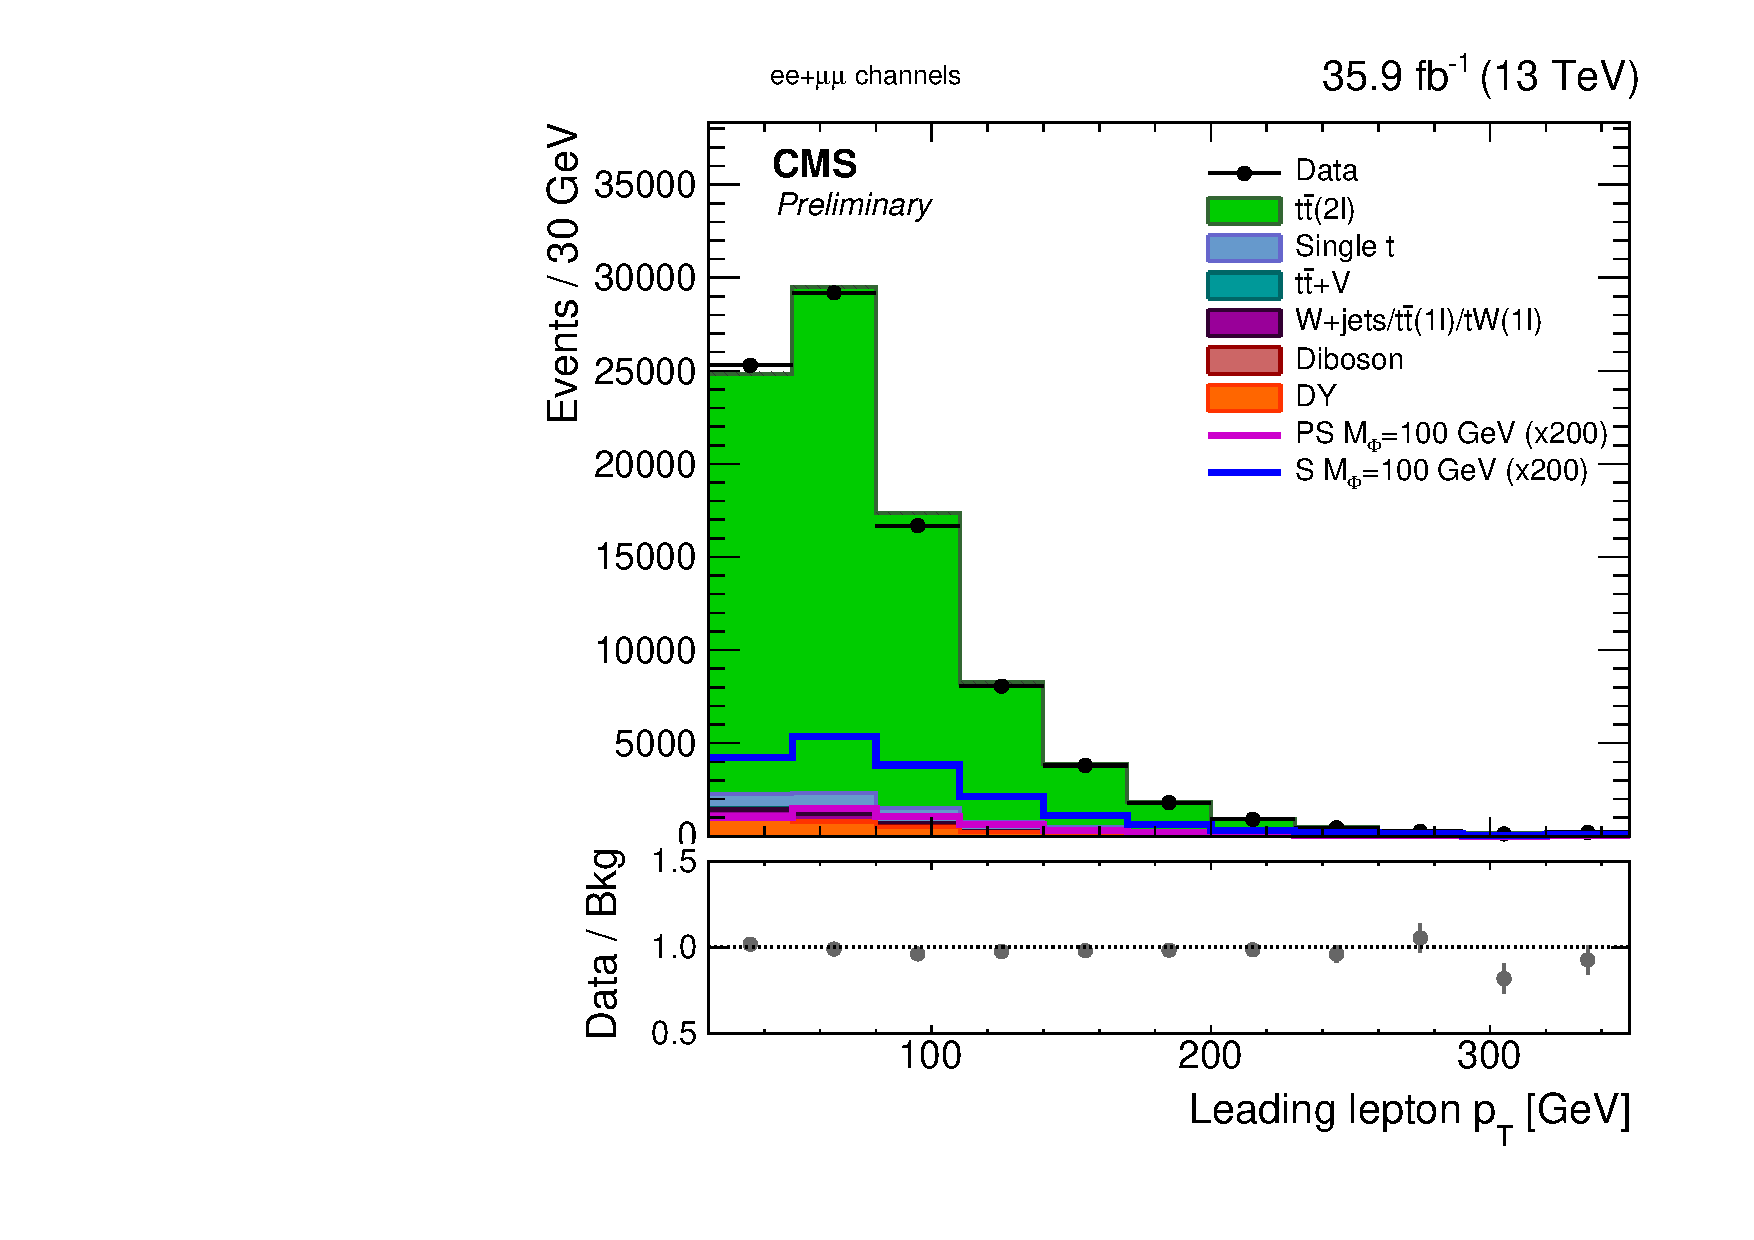
\includegraphics[width=0.43\textwidth]{figs/inclusiveSR/lep1pt_sf.pdf}}
  \subfloat[leading lepton $\eta$] {\label{subfig:lepeta_sf}   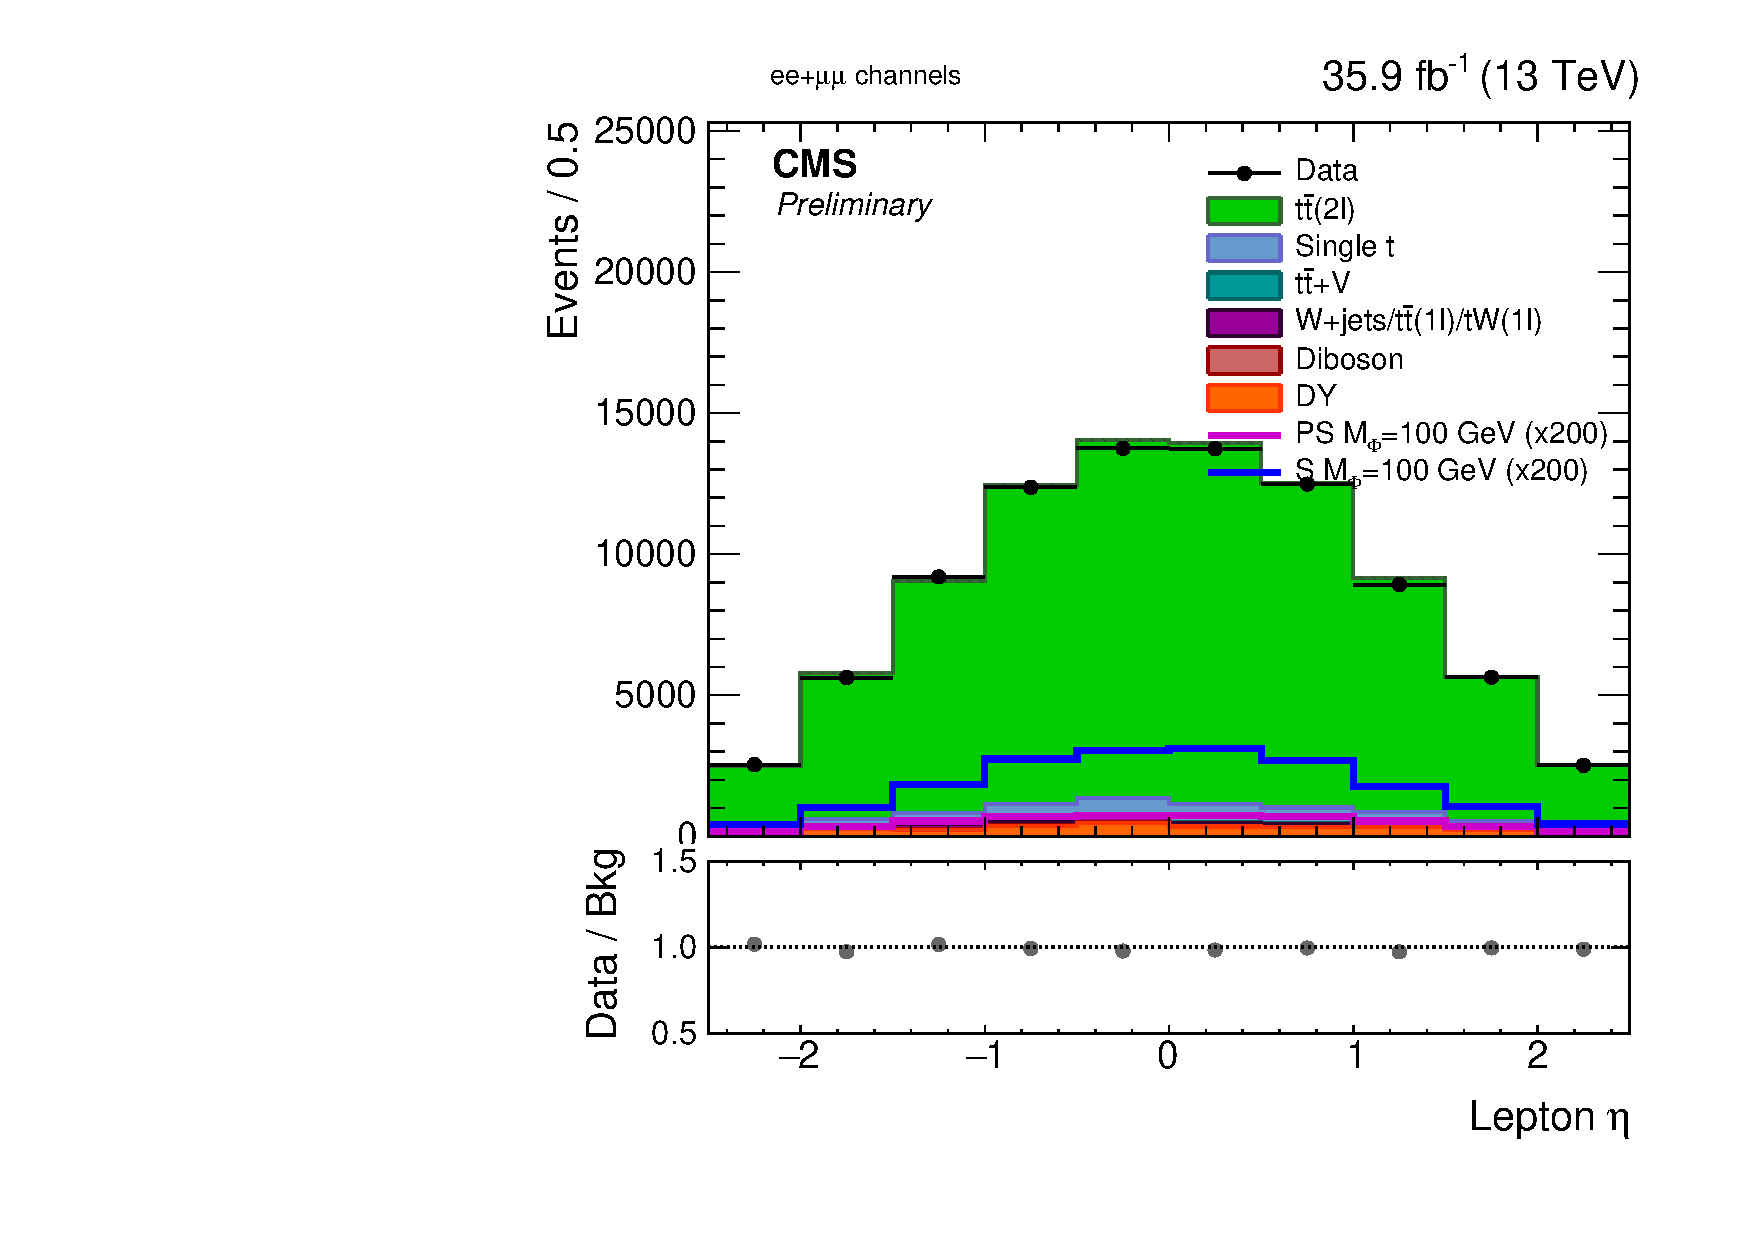
\includegraphics[width=0.43\textwidth]{figs/inclusiveSR/lep1eta_sf.pdf}} \\
  \subfloat[leading jet $\pt$]     {\label{subfig:jetpt_sf}    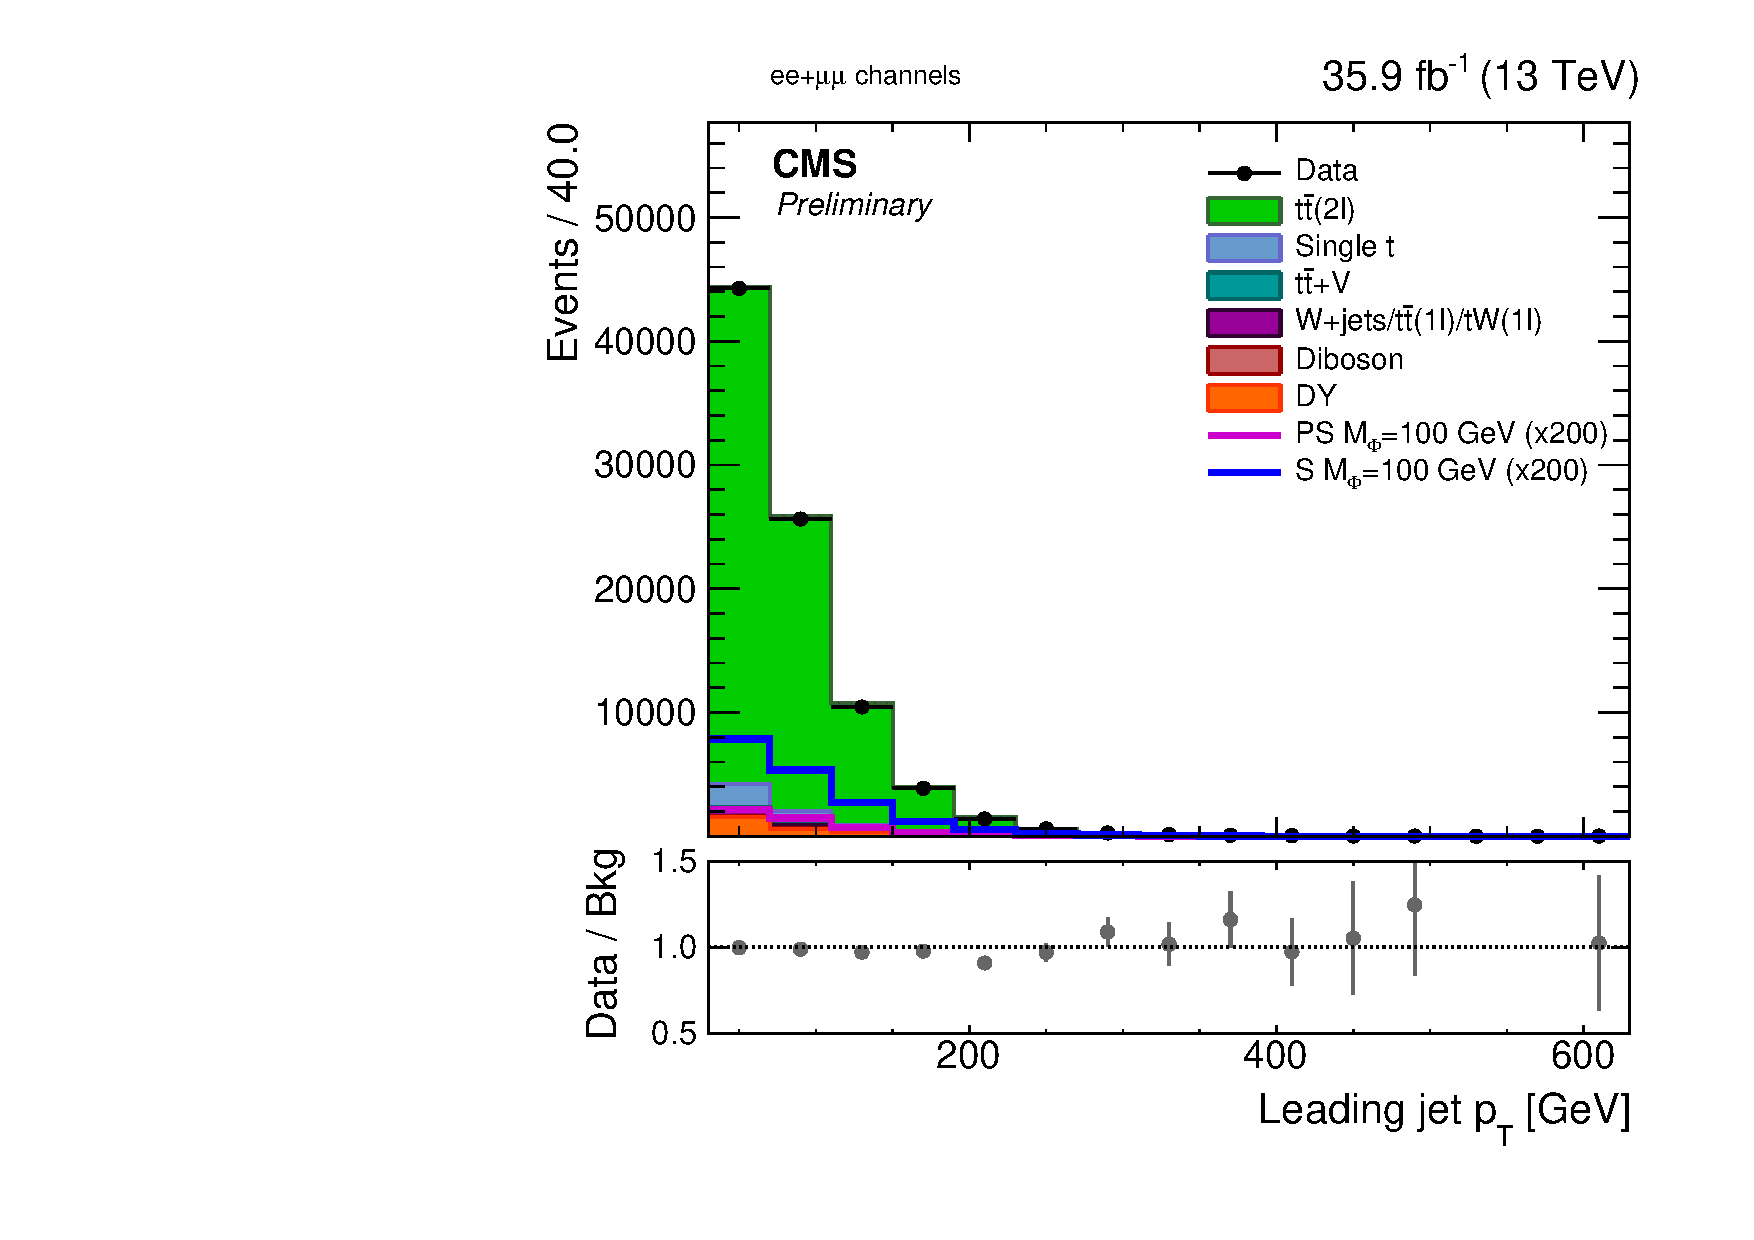
\includegraphics[width=0.43\textwidth]{figs/inclusiveSR/jet1pt_sf.pdf}}
  \subfloat[leading jet $\eta$]    {\label{subfig:jeteta_sf}   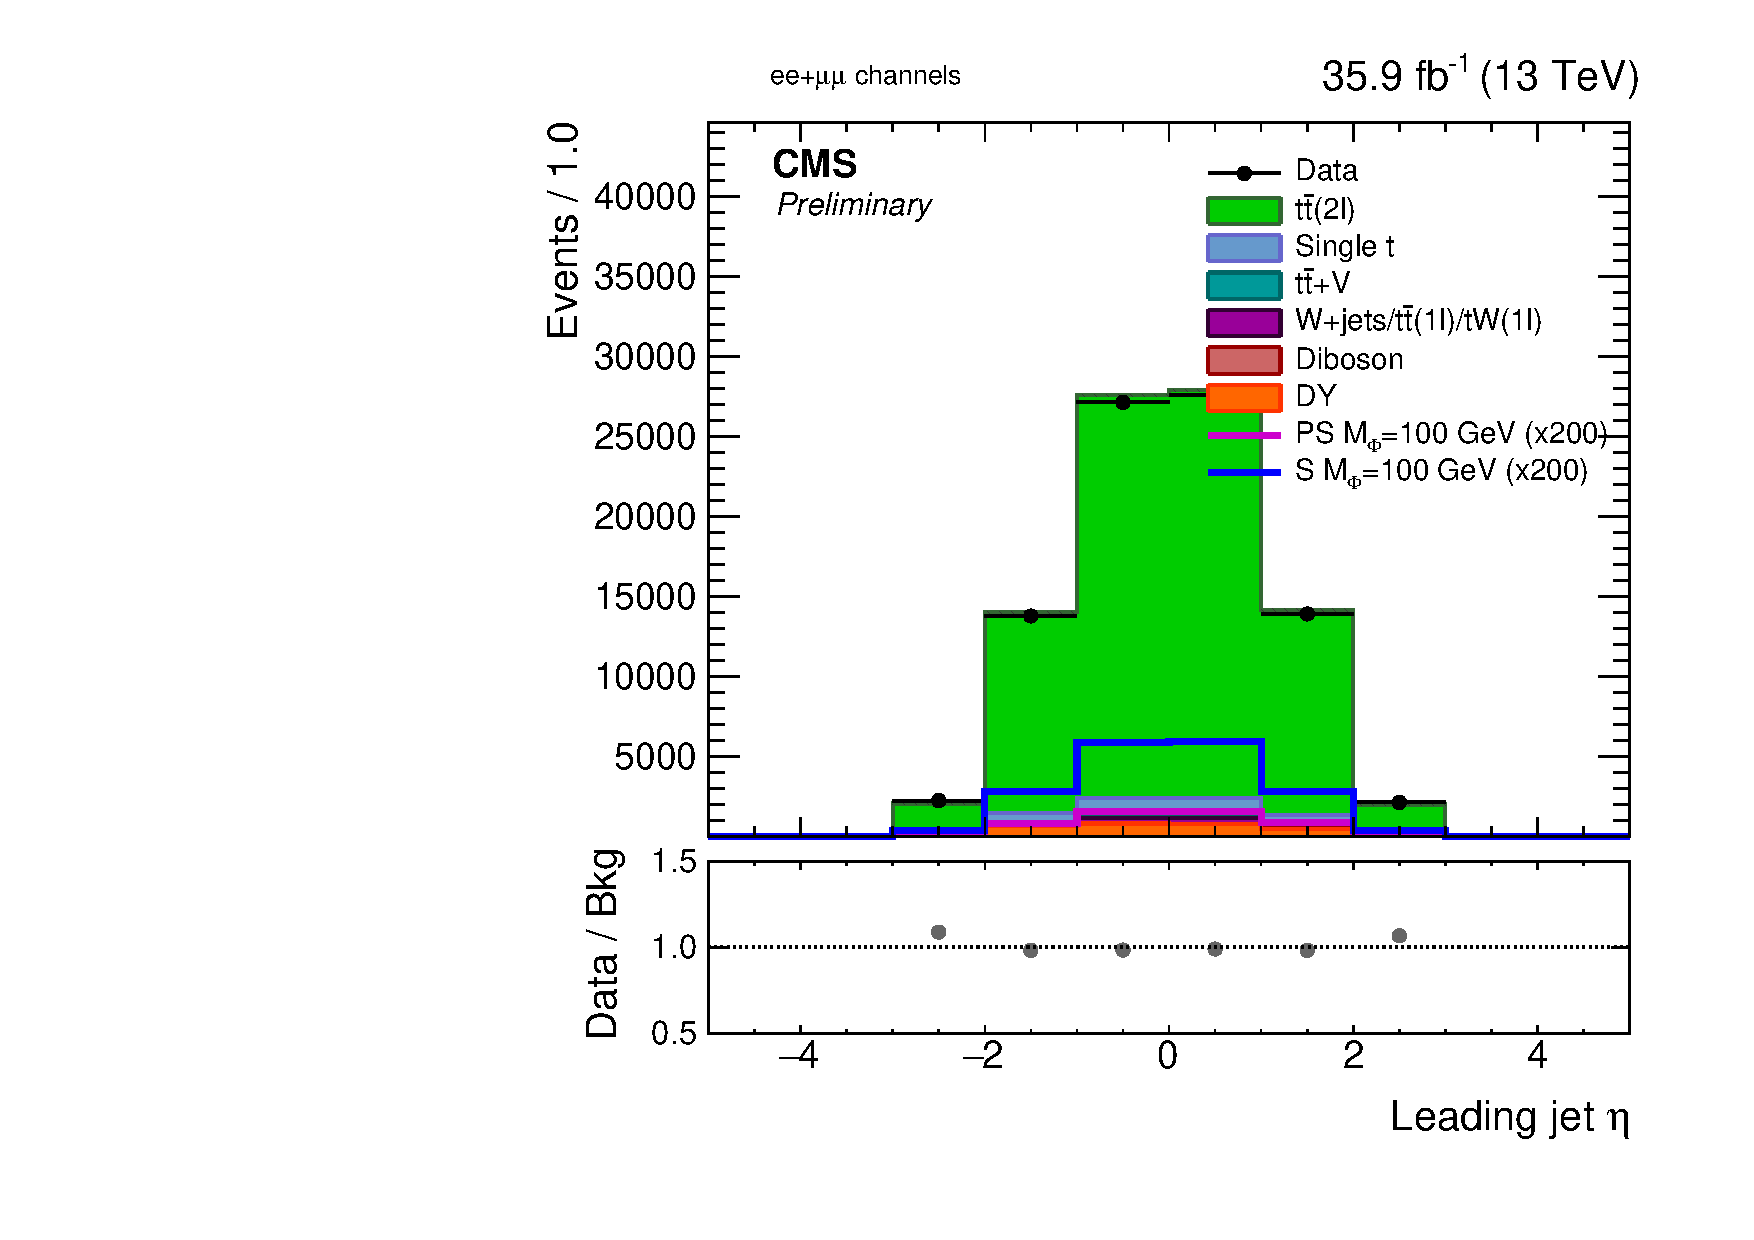
\includegraphics[width=0.43\textwidth]{figs/inclusiveSR/jet1eta_sf.pdf}}
  \caption{}
  \label{fig:dilep_sr_sf}
\end{figure}

\begin{figure}[h!]
  \ContinuedFloat
  \centering
  \subfloat[$\pt^{\ell\ell}$]                  {\label{subfig:dileppt_sf}  \includegraphics[width=0.43\textwidth]{figs/inclusiveSR/dileppt_sf.pdf}}
  \subfloat[$m_{\ell\ell}$]                    {\label{subfig:dilepmass_sf}\includegraphics[width=0.43\textwidth]{figs/inclusiveSR/dilepmass_sf.pdf}} \\
  \subfloat[$\Delta\phi(\ell\ell,\ptvecmiss)$] {\label{subfig:dphidilepmet_sf}  \includegraphics[width=0.43\textwidth]{figs/inclusiveSR/dphidilepmetlog_sf.pdf}}
  \subfloat[\ptmiss]                           {\label{subfig:met_sf}\includegraphics[width=0.43\textwidth]{figs/inclusiveSR/metlog_sf.pdf}}
  \caption{Kinematic distributions in the same flavor ($ee+\mu\mu$) channel. Signals with a pseudoscalar (magenta) and scalar (blue) mediator with $\mMed=100\:\GeV$ and $\mDM=1\:\GeV$ are overlayed and scaled by a factor of 200 to illustrate the potential shape differences between the signal and background in the various distributions. The uncertainties shown in these plots on the data and background are purely statistical.}
  \label{fig:dilep_sr_sf}
\end{figure}

\begin{figure}[h!]
  \centering
  \subfloat[$N_{\textrm{jets}}$]   {\label{subfig:njets_em}    \includegraphics[width=0.43\textwidth]{figs/inclusiveSR/njets_em.pdf}}
  \subfloat[$N_{\textrm{b-jets}}$] {\label{subfig:nbjets_em}   \includegraphics[width=0.43\textwidth]{figs/inclusiveSR/nbjetsm_em.pdf}} \\
  \subfloat[leading lepton $\pt$]  {\label{subfig:leppt_em}    \includegraphics[width=0.43\textwidth]{figs/inclusiveSR/lep1pt_em.pdf}}
  \subfloat[leading lepton $\eta$] {\label{subfig:lepeta_em}   \includegraphics[width=0.43\textwidth]{figs/inclusiveSR/lep1eta_em.pdf}} \\
  \subfloat[leading jet $\pt$]     {\label{subfig:jetpt_em}    \includegraphics[width=0.43\textwidth]{figs/inclusiveSR/jet1pt_em.pdf}}
  \subfloat[leading jet $\eta$]    {\label{subfig:jeteta_em}   \includegraphics[width=0.43\textwidth]{figs/inclusiveSR/jet1eta_em.pdf}}
  \caption{}
  \label{fig:dilep_sr_em}
\end{figure}

\begin{figure}[h!]
  \ContinuedFloat
  \centering
  \subfloat[$\pt^{\ell\ell}$]                  {\label{subfig:dileppt_em}  \includegraphics[width=0.43\textwidth]{figs/inclusiveSR/dileppt_em.pdf}}
  \subfloat[$m_{\ell\ell}$]                    {\label{subfig:dilepmass_em}\includegraphics[width=0.43\textwidth]{figs/inclusiveSR/dilepmass_em.pdf}} \\ 
  \subfloat[$\Delta\phi(\ell\ell,\ptvecmiss)$] {\label{subfig:dphidilepmet_em}  \includegraphics[width=0.43\textwidth]{figs/inclusiveSR/dphidilepmetlog_em.pdf}}
  \subfloat[\ptmiss]                           {\label{subfig:met_em}\includegraphics[width=0.43\textwidth]{figs/inclusiveSR/metlog_em.pdf}}
  \caption{Kinematic distributions in the same flavor ($e\mu$) channel. Signals with a pseudoscalar (magenta) and scalar (blue) mediator with $\mMed=100\:\GeV$ and $\mDM=1\:\GeV$ are overlayed and scaled by a factor of 200 to illustrate the potential shape differences between the signal and background in the various distributions. The uncertainties shown in these plots on the data and background are purely statistical.}
  \label{fig:dilep_sr_em}
\end{figure}

\begin{figure}[h!]
  \subfloat[][$ee+\mu\mu$ channel] {\label{subfig:mt2ll_sf} \includegraphics[width=0.48\textwidth]{figs/inclusiveSR/mt2log_sf.pdf}} 
  \subfloat[][$e\mu$ channel]      {\label{subfig:mt2ll_em} \includegraphics[width=0.48\textwidth]{figs/inclusiveSR/mt2log_em.pdf}} 
  \caption{The \mttll distribution in the~\protect\subref{subfig:mt2ll_sf} same flavor and~\protect\subref{subfig:mt2ll_em} opposite flavor channels. Events with \mttll below (above) $110\:\GeV$ form the low (high) signal purity categories. The uncertainties in the above plots are statistical only. The \mttll templates for signals with a pseudoscalar (magenta) and scalar (blue) mediator with $\mMed=100\:\GeV$ and $\mDM=1\:\GeV$ are overlayed and scaled by a factor of 200.}
  \label{fig:mt2_sr}
\end{figure}

\begin{figure}[h!]
  \subfloat[][low purity: $ee+\mu\mu$] {\label{subfig:metlo_sf} \includegraphics[width=0.48\textwidth]{figs/cat-lo_metlog_ll.pdf}}
  \subfloat[][low purity: $e\mu$]      {\label{subfig:metlo_em} \includegraphics[width=0.48\textwidth]{figs/cat-lo_metlog_em.pdf}}
  \caption{The \ptmiss distributions in the low purity signal region for~\protect\subref{subfig:metlo_sf} same flavor and~\protect\subref{subfig:metlo_em} opposite flavor events. The uncertainties in the above plots are statistical only. The \ptmiss templates in the low purity signal region for signals with a pseudoscalar (magenta) and scalar (blue) mediator with $\mMed=100\:\GeV$ and $\mDM=1\:\GeV$ are overlayed and scaled by a factor of 200.}
  \label{fig:metlo}
\end{figure}

\begin{figure}[h!]
  \subfloat[][high purity: $ee+\mu\mu$] {\label{subfig:methi_sf} \includegraphics[width=0.48\textwidth]{figs/cat-hi_metlog_ll.pdf}}
  \subfloat[][high purity: $e\mu$]      {\label{subfig:methi_em} \includegraphics[width=0.48\textwidth]{figs/cat-hi_metlog_em.pdf}}
  \caption{The \ptmiss distributions in the high purity signal region for~\protect\subref{subfig:methi_sf} same flavor and~\protect\subref{subfig:methi_em} opposite flavor events. The uncertainties in the above plots are statistical only. The \ptmiss templates in the high purity signal region for signals with a pseudoscalar (magenta) and scalar (blue) mediator with $\mMed=100\:\GeV$ and $\mDM=1\:\GeV$ are overlayed and scaled by a factor of 200.}
  \label{fig:methi}
\end{figure}

%\vspace*{0.5\textheight}

\section{Systematic uncertainties}
\label{sec:systunc}

The signal and background \ptmiss templates derived from simulation are subject to effects incurred from experimental and theoretical sources of uncertainty. The \ptmiss distributions are parametrized in order to allow for constrained shape and normalization variations as a cause of the systematic uncertainties, referred to throughout as ``systematics''. Each systematic is represented by a nuisance parameter, $\theta$, with a probability density function, $pdf$, denoted as $\rho(\theta)$, that contains the central value of the nuisance, $\widetilde{\theta}$, and other parameters that describe the overall shape of the $pdf$, such as its width. 

Uncertainties which affect the normalization of the signal and background processes are modeled using nuisance parameters with log-normal probability densities. The log-normal $pdf$ follows the form~\cite{CMS-NOTE-2011-005},

\begin{equation}
  \rho(\theta) = \frac{1}{\sqrt{2\pi}\ln{\kappa}}\exp{\bigg(-\frac{(\ln{(\theta/\widetilde{\theta})})^2}{2(\ln{\kappa})^2}\bigg)}\frac{1}{\theta}.
\end{equation}

where the width of the log-normal distribution is characterized by $\kappa$, and $\widetilde{\theta}$ represents the best estimate of the nuisance $\theta$. In the limit of small uncertaint ($\epsilon$), the width of a Gaussian $pdf$ is given by $\sigma=\epsilon$, which equates directly to the log-normal width via a Taylor expansion for $\kappa = e^{\epsilon}$, such that $\kappa=1+\epsilon$. The log-normal $pdf$ is useful in the case of large uncertainties as the distribution has a longer tail in comparison with a Gaussian $pdf$, and avoids the problem of negative parameter values obtained from a Gaussian probability density, since $\rho(\theta)\rightarrow0$ for $\theta=0$.

A number of uncertainties influence the overall shape of the signal and background \ptmiss templates along with the normalization. Systematics of this type are implemented using a general technique known as ``vertical morphing''~\cite{Conway:2011in}. A change in a particular type of uncertainty (such as an energy scale) can cause a distortion in both the shape and overall normalization of the efficiency as a function of the observable (\ptmiss) bin. Raising and lowering a particular parameter to its corresponding values at one standard deviation will cause the bin efficiencies, denoted as $\epsilon_{ij}$ for source $i$ in observable bin $j$, to also shift, thus resulting in three measures of the bin efficiency shape, referred to as $\epsilon^{+}_{ij}$, $\epsilon^{0}_{ij}$, and $\epsilon^{-}_{ij}$. In order to transform the three shape measures into a continuous estimate as a function of the parameter value, a morphing parameter, represented by $f$ and nominally equal to 0 with a unitary uncertainty, is used. A quadratic interpolation is used for values where $|f|<1$, to express the efficiency in a bin as a function of the morphing parameter such that, 

\begin{equation}
  \epsilon_{ij} = \frac{f(f-1)}{2}\epsilon^{-}_{ij} - (f-1)(f+1)\epsilon^{0}_{ij} + \frac{f(f+1)}{2}\epsilon^{+}_{ij}.
  \label{eq:morph}
\end{equation}

The form of Eq.~\ref{eq:morph} guarantees that the value of the expression is $\epsilon^{\pm}_{ij}$ for $f=\pm 1$. 

\subsection{Sources of systematic uncertainty}

The following sources of uncertainty affect the normalization of the signal and background processes: 

\begin{itemize}
  \item \textbf{Pileup modeling}: As described in Sec.~\ref{subsec:pu}, the total inelastic cross section used to calculate the data pileup distributions is varied by $\pm4.6\%$, in order to account for systematic uncertainties due to pileup modeling. Normalization differences in the range of $0.3-11\%$ result from reweighting the simulation accordingly.
  \item \textbf{Integrated luminosity}: The overall uncertainty of the measurement of the integrated luminosity delivered to the CMS Experiment during the 2016 LHC proton-proton run at $\sqrt{s}=13\:\TeV$ is estimated to be $2.5\%$~\cite{CMS-PAS-LUM-17-001}.
  \item \textbf{Lepton reconstruction and selection}: The uncertainty on lepton reconstruction and selection efficiency is associated with the efficiency measurement with samples of Z bosons decaying to dielectrons or dimuons~\cite{CMS:2011aa}. The $\pt$- and $\eta$-dependent scale factors are varied within their uncertainties which amounts to $\approx 2\%$ per lepton.
  \item \textbf{Lepton trigger}: The uncertainty on lepton triggering efficiency is associated with the efficiency measurement with samples of Z bosons decaying to dielectrons or dimuons. The corresponding uncertainty ranges from $1\%$ to $2\%$.
  \item \textbf{b-tagging efficiency}: The b-tagging efficiency and mis-tag rate and the respective uncertainties are measured on independent control samples. Uncertainties from gluon splitting, the b quark fragmentation function, and the selections used to define the control samples are propagated to the efficiency scale factors~\cite{CMS-PAS-BTV-15-001}. The uncertainties on the mis-tag rate range from $0.1-4\%$, while the b-tagging efficiency uncertainties range from $0.1-2\%$.
  \item \textbf{Single top and diboson normalization}: In practice, the expected yields for background processes are either scaled to data or to theory predictions with the best available accuracy. The uncertainties on the cross section predictions are taken into account in the PDF as well as the renormalization and factorization scale uncertainties. However, in the single top and diboson simulation samples used, the aforementioned variations are not available, so a conservative uncertainty of $20\%$ and $10\%$ is assigned respectively to the normalizations, and these uncertainties are treated independently of eachother.  
\item \textbf{Drell-Yan background uncertainty}: The uncertainties incurred from the data-driven estimate of the Drell-Yan background normalization are dominated by the statistical uncertainties on $N_{\mbox{\tiny{in}}}$ and $R^{1b}_{\mbox{\tiny{MC}}}$, quantities used to extrapolate yields from a region near the Z boson mass to regions away from it, as described in Sec.~\ref{sec:DY}. The uncertainties are $11\%$ and $6\%$ for the $ee$ and $\mu\mu$ channels and only applies to the DY background.
\item \textbf{Fake lepton background uncertainty}:
The sources of uncertainty in the fake lepton background stem from the uncertainty in the measured fake rate, and from the statistical uncertainty of the single-lepton control sample to which the rate is applied, as described in Sec.~\ref{sec:fakes}. The uncertainties are $78\%$ ($ee$), $70\%$ ($e\mu$), $74\%$ ($\mu\mu$) in the high signal purity category and $47\%$ ($ee$), $12\%$ ($e\mu$), and $20\%$ ($\mu\mu$) in the low signal purity category, and are dominated by the statistical uncertainty associated with the single-lepton control sample. Since the fake lepton background is small, these relatively large uncertainties do not significantly degrade the sensitivity of the search.
\end{itemize}

The systematics affecting the overall \ptmiss shape and normalization listed below in order of decreasing dominance on the final result:

\begin{itemize}
  \item \textbf{Jet energy scale (JES)}: Reconstructed jet four-momenta in the simulation are simultaneously varied according to the uncertainty on the JES. JES uncertainties are coherently propagated to all observables impacted, including jet kinematics and multiplicity, \ptmiss, and \mttll. Uncertainty effects due to the jet energy resolution (JER) were found to be negligible.
\item \textbf{Fake \ptmiss uncertainty}:
For the high signal purity ($\mttll > 110\:\GeV$) category, an uncertainty is assigned to the background \ptmiss shapes derived from simulation to account for potential mismodeling of the rate of events with large fake \ptmiss in simulation. This uncertainty is derived using Z bosons decaying to dielectrons and dimuons, as a function of hadronic recoil (i.e. \ptmiss with the two leptons removed), and also passing $\mttll > 110\:\GeV$. The difference between the simulation and data after the subtraction of non-Drell-Yan events as expected from simulation, is taken as the uncertainty and added/subtracted to the nominal recoil distribution to obtain the one standard deviation variations. A second-order polynomial is fit to the fake \ptmiss uncertainty scale factor distributions in an effort to smoothen the uncertainty as a function of the recoil, as shown in ~\FigureRef{fig:recoilSF}. 
\item \textbf{Factorization and renormalization scales}:
Uncertainties due to the renormalization scale $\mu_R$ and the factorization scale $\mu_F$ employed in the simulation matrix-element generator are modeled by halving or doubling  each of the scales independently~\cite{Collins:1989gx}, and propagating the changes to the \ptmiss templates. This is accommodated via weights obtained directly from the generator information in the MC simulation where available. The uncertainty is considered to be uncorrelated among the different background processes. 
\item \textbf{Top quark \pt reweighting}: 
The top quark \pt spectrum as measured in differential top quark pair production is observed to be softer than that of simulation, as discussed in Sec.~\ref{subsec:toppt}. In order to cover this effect, the scale factors derived in previous CMS measurements~\cite{Khachatryan:2016mnb} are applied to the \ttbar simulation by default. The uncertainty is estimated from a comparison of the top \pt spectrum obtained without the reweighting applied.
\item \textbf{Parton distribution function (PDF)}: Uncertainties due to the choice of PDFs used to simulate the hard scatter process are estimated by reweighting the simulation samples with the ensemble of 100 PDF replicas~\cite{0954-3899-43-2-023001} provided by NNPDF3.0~\cite{Ball:2014uwa}.
\end{itemize}

\begin{figure}[h!] 
  \centering
  \includegraphics[width=0.6\textwidth]{figs/RecoilUpFit.png}
  \caption{The fake \ptmiss uncertainty at one standard deviation from the nominal recoil distribution as derived in simulation using Z bosons decaying to dielectrons and dimuons with $\mttll > 110\:\GeV$. In order to smoothen out the binned uncertainty, it is fit with a second-order polynomial.}
  \label{fig:recoilSF}
\end{figure}

\section{Statistical analysis}
\label{sec:stats}
The methods by which the statistical analysis is performed are outlined in the following section. A brief description of the model parameter estimation and statistical model inference methods are outlined. Finally, the means by which the signal is extracted is described. An in-depth discussion of statistical methods can be found in 

\subsection{Maximum likelihood}
\label{subsec:maxlikelihood}
The maximum likelihood estimates the best value of the parameters (i.e. signal strength and background shape and normalizations), for which the observed data has the highest probability of estimating the true parameter value according to the hypothesis model. Following the discussion in~\cite{}, supposing in a set of $N$ events, we observe a set of measured quanties, $\bar{x}$. In the space of these observables we can define a set of bins, $n_{bin}$, and it is assumed that the number of events $n_{i}$ in each bin $i$ are Poisson-distributed such that,

\begin{equation}
  \mathcal{P}(n_{i}\mid\lambda_{i}) = \frac{\lambda_{i}^{n_{i}}e^{-\lambda_{i}}}{n_{i}!},
\end{equation}

where $\lambda_{i}$ is the number of expected events in the bin containing contributions from both signal and background processes such that $\lambda = \mu s + b$. The number of signal (background) events is denoted by $s$ ($b$), and subsequently the parameter $\mu$ represents the signal strength scaling, where $\mu=0$ corresponds to the background-only hypothesis, and $\mu=1$ is the nominal signal hypothesis. The likelihood function is then simply the product of Poisson probabilities for all bins,

\begin{equation}
  \mathcal{L} = \prod_{j=1}^{N}\frac{(\mu s_{j}+b_{j})^{n_j}}{n_{j}!}e^{-(\mu s_j + b_j)},
  \label{eq:like}
\end{equation}

where the mean number of entries in the $j$th bin from signal and background are

\begin{equation}
  s_{j}  = s_{\textrm{tot}}\int_{\textrm{bin j}} f_{s}(x;\textbf{\theta}_{s})dx, 
\label{eq:sigpdf}
\end{equation}

\begin{equation}
  b_{j}  = b_{\textrm{tot}}\int_{\textrm{bin j}} f_{b}(x;\textbf{\theta}_{b})dx. 
\label{eq:bkgpdf}
\end{equation}

The functions $f_{s}(x;\textbf{\theta}_{s})$ and $f_{b}(x;\textbf{\theta}_{b})$ are the $pdf$s of the variable $x$ for signal and background events and $\textbf{\theta}_s$ and $\textbf{\theta}_b$ are the nuisance parameters described in Sec.~\ref{sec:systunc}, which characterize the shape of the $pdf$s. The integrals in Eq.~\ref{eq:sigpdf} and Eq.~\ref{eq:bkgpdf} represent the probabilities for an event to be found in bin $j$, and $s_\mathrm{tot}$ and $b_\mathrm{tot}$ denote the total mean numbers of signal and background events, respectively. It is then clear that the likelihood in Eq.~\ref{eq:like} is a function of the nuisance parameters, $\mathcal{L}(\textbf{\theta})$, and the values of $\textbf{\theta}$ which maximize this quantity are said to fit the observation best.

\subsection{Hypothesis testing}
\label{subsec:hypothesis}

In order to determine whether to accept or reject a model depending on the outcome of a measurement, a frequentist test of a hypothesis is performed. In this case, we test the hypothesized value of the signal strength, $\mu$, which is interpreted as the ratio of the measured cross section, $\sigma$, to the predicted value from the theory model, $\sigma_{\textrm{TH}}$, such that $\mu=\frac{\sigma}{\sigma_{\textrm{TH}}}$. Hence, a null value of $\mu$ corresponds to an observation compatible with the SM background-only hypothesis, whereas if the observation is compatible with signal events as predicted by the model cross section, then $\mu=1$. 

Quantifying the level of agreement between the observation and a tested hypothesis is done via a test statistic $q(\mu)$, which is defined as the ratio of maximum likelihoods,

\begin{equation}
  q(\mu) = \frac{\mathcal{L}(\mathcal{D}\mid\mu,\hat{\hat{\textbf{\theta}}}(\mu))}{\mathcal{L}(\mathcal{D}\mid\hat{\mu},\hat{\textbf{\theta}})}
  \label{eq:proflikelihood}
\end{equation}

where the $\hat{\hat{\textbf{\theta}}}(\mu)$ indicates the values of the nuisance parameters $\textbf{\theta}$ profiled, which maximize $\mathcal{L}$ for a fixed value of $\mu$, the dataset $\mathcal{D}$, and global observables. The denominator of the so-called \textit{profile likelihood ratio} defined by Eq.~\ref{eq:proflikelihood} is the value of $\mathcal{L}$ when evaluated with the maximum likelihood estimators (MLEs) $\hat{\mu}$ and $\hat{\textbf{\theta}}$. The MLEs and profiled nuisance parameters can analogously minimize the quantity $-2\ln{\mathcal{L}}$, so it is common to write the definition of the test statistic as,

\begin{equation}
   q(\mu) = -2\ln{\frac{\mathcal{L}(\mu,\hat{\hat{\textbf{\theta}}}(\mu))}{\mathcal{L}(\hat{\mu},\hat{\textbf{\theta}})}}, \mu' \leq \mu.
   \label{eq:likelihood}
\end{equation}

For the purposes of setting limits on theoretical parameters (i.e. determining the values of the parameters that are allowed or excluded given the available data) the test statistic $q(\mu)$ is used to discriminate between the hypothesis of the signal being produced at a rate $\mu$ from an alternative hypothesis of signal events being produced at a lesser rate $\mu' < \mu$. Thus, it is a test statistic for a one-sided alternative or moreover provides a one-sided upper limit. If the experiment were to be repeated multiple times, $q(\mu)$ would take on different values, thus the test statistic itself has a particular probability density function, $f(q(\mu)\mid H)$, dependent on the particular hypothesis, $H$, being tested. Then the probability that a given $q(\mu)_{\textrm{obs}}$ is an equal or more 'extreme' outcome than observed, assuming $H$ is,

\begin{equation}
  p = \int_{q(\mu)_{\textrm{obs}}}^{\infty} f(q(\mu)\mid H)\xspace dq(\mu).
\label{eq:pvalue}
\end{equation}

The quantity in Eq.~\ref{eq:pvalue} and visualized in Fig.~\ref{fig:pvalues}, known as the \textit{p-value}, indicates a worse agreement with the corresponding $H$ for small $p$-values. In the language of discovery in high energy physics, it is customary to relate the $p$-value into a quantile of a unit Gaussian to express the significance $Z$, as shown in Fig.~\ref{fig:pvalues}. The area of the tail starting at an upward fluctuation of $Z$ standard deviations from the mean of the Gaussian random variable, should be equal to the $p$-value. The transformation is defined formally as, 

\begin{equation}
  Z = \Phi^{-1}(1-p)
\end{equation}

where $\Phi^{-1}$ is the inverse of the cumulative distribution of the signle sided standard Gaussian. A $5\sigma$ significance is the common requirement to claim a discovery, which is analogous to a $p$-value of $2.87 \times 10^{-7}$.

\begin{figure}[htbp!]
  \subfloat[][]{\label{subfig:pvalue}\includegraphics[width=0.4\textwidth]{figs/pvalue.png}}
  \subfloat[][]{\label{subfig:sig}   \includegraphics[width=0.4\textwidth]{figs/significance.png}}
  \caption{A visualization of the relation~\protect\subref{subfig:pvalue} between the observed value of the test statistic $q(\mu)_{\textrm{obs}}$, the probability density function $f(q(\mu)\mid H)$ and the $p$-value, and~\protect\subref{subfig:sig} between the $p$-value and the signficance $Z$.}
  \label{fig:pvalues}
\end{figure}

In the absence of a discovery, i.e. the $p$-value determined from the observed data cannot exclude the background-only hypothesis, then the upper limit on the signal strength parameter, $\mu$, is established. The one-sided modified frequentist confidence level ($\textrm{CL}_s$) upper limit on $\mu$ is defined as,

\begin{equation}
  \textrm{CL}_{s} = \frac{p_\mu}{1-p_0}
  \label{eq:CLs}
\end{equation} 

where $p_{0}$ is the $p$-value determined given that the hypothesis under test is that of the SM background-only. In practice, results are calculated at $95\%$ $\textrm{CL}_s$ which is defined as the $\mu$ that produces $\textrm{CL}_s=0.05$.

\subsection{Signal extraction}
\label{subsec:signal}

An excess of events in the dataset with respect to the expected SM predictions would indicate the presence of the \ttDM signal process. In order to extract the results, a binned maximum likelihood fit is performed simultaneously on the \ptmiss distributions in the SRs as defined in more detail in Sec.~\ref{sec:observables}. A single strength parameter is used to scale the signal across all the SRs. The sources of systematic uncertainties are represented by nuisance parameters in the fit, as described in greater detail in Sec.~\ref{sec:systunc}.

The likelihood ratio defined by Eq.~\ref{eq:likelihood} is used to assess the fit for the saturated model, and provides a generalization of the $\chi^2$ goodness-of-fit test as per~\cite{BAKER1984437}. The fitted background-only \ptmiss distributions are shown in~\FigureRef{fig:postfit_lo} and~\FigureRef{fig:postfit_hi}. The corresponding observed data yield and post-fit SM background expected yields are presented for the high and low purity categories in Table~\ref{tab:cat-hi_postfit_yields} and~\ref{tab:cat-lo_postfit_yields}, respectively. The $p$-value of 0.06, as defined by Eq.~\ref{eq:pvalue}, is determined from the distribution of the likelihood ratio obtained from pseudodata generated from the fitted simulation yields. No significant excess in the SRs is observed. 

\begin{table}[!htbp]
\caption{Background-only post-fit event yields passing selection in the $M_{T2}^{\ell\ell}>110\:\GeV$ (high signal purity) category. The expected (pre-fit) yield is also shown for a pseudoscalar $m_a=100\:\GeV,\,m_\chi=1\:\GeV$ signal. The uncertainties include contributions from both systematic and statistical sources.}
\label{tab:cat-hi_postfit_yields}
\centering
\begin{tabular}{l|r|r}
\hline
\multicolumn{3}{c}{\mttll$>110\:\GeV$} \\
\hline
                            & \multicolumn{1}{c|}{$ee+\mu\mu$} & \multicolumn{1}{c}{$e\mu$} \\
\hline
  Diboson                   &  $3.83 \pm   0.51$        &  $1.42 \pm   0.58$          \\
  Drell-Yan                 &  $68.51 \pm   9.88$       &  $0.85 \pm   0.51$          \\
  Single t ($2\ell$)        &  $7.34 \pm   1.51$        &  $8.59 \pm   1.88$          \\
  $\ttbar+V$                &  $7.83 \pm   1.12$        &  $5.87 \pm   0.95$          \\
  $\ttbar(2\ell)$           &  $77.67 \pm   5.60$       &  $104.91 \pm 7.49$          \\
  Fakes                     &  $0.72 \pm   0.92$        &  $4.14 \pm   2.82$          \\
\hline
  SM Expected               & $165.90 \pm 10.26$        & $125.77 \pm 8.96$            \\
  Observed                  & $156$                     & $128$                        \\
  $m_a=100,\,m_\chi=1$      & $5.18 \pm  0.089$         & $5.82 \pm  0.094$            \\
\hline
\end{tabular}
\end{table}

\begin{table}[!ht]
\caption{Background-only post-fit event yields passing selection in the $M_{T2}^{\ell\ell}<110\:\GeV$ (low signal purity) category. The expected (pre-fit) yield is also shown for a pseudoscalar $m_a=100\:\GeV,\,m_\chi=1\:\GeV$ signal. The uncertainties include contributions from both systematic and statistical sources.}
\label{tab:cat-lo_postfit_yields}
\centering
\begin{tabular}{l|r|r}
\hline
\multicolumn{3}{c}{\mttll$<110\:\GeV$} \\
\hline
                           & \multicolumn{1}{c|}{$ee + \mu\mu$} & \multicolumn{1}{c}{$e\mu$} \\
\hline
  Diboson                  &  $178.05 \pm  10.85$     &    $148.68 \pm   9.19$     \\
  Drell-Yan                &  $2633.18 \pm 279.35$    &    $267.71 \pm  29.52$     \\
  Single t ($2\ell$)       &  $3356.63 \pm 553.19$    &  $3946.44 \pm 648.20$    \\
  $\ttbar+V$               &  $232.94 \pm  31.56$     &   $256.39 \pm  33.33$     \\
  $\ttbar(2\ell)$          &  $79534.15 \pm 702.17$   & $94338.27 \pm 805.11$    \\
  Fakes                    &  $689.18 \pm 322.88$     &   $792.42 \pm  80.64$    \\
\hline
  SM Expected              & $86624.13 \pm 401.67$      & $ 99749.92 \pm 469.50$ \\
  Observed                 & $86619$                    & $99793$                \\
  $m_a=100,\,m_\chi=1$     & $19.63 \pm  0.17$          & $22.70 \pm  0.19$      \\
\hline
\end{tabular}
\end{table}

\begin{figure}[htbp!]
  \subfloat[][low purity, $ee+\mu\mu$ channel]{\label{subfig:postfit_lo_sf}\includegraphics[width=0.48\textwidth]{figs/postfit/metlog_shapes_fit_b_dl_lo_mt2_ll.pdf}}
  \subfloat[][low purity, $e\mu$ channel]     {\label{subfig:postfit_lo_of}\includegraphics[width=0.48\textwidth]{figs/postfit/metlog_shapes_fit_b_dl_lo_mt2_em.pdf}}
  \caption{The background-only post-fit \ptmiss distributions in the low signal purity SRs. The expected (pre-fit) \ptmiss distributions for two example signals (scalar and pseuscalar mediator, $m_{\phi/a}=100\:\GeV$) with $m_{\chi}=1\:\GeV$ are scaled up by a factor of 200. The dashed blue line represents the total expected (pre-fit) MC background \ptmiss shape, and the subsequent ratio between the pre-fit and post-fit shape in the lower ratio panel. The last bin of the distributions includes overflow. Statistical and systematic uncertainties are shown.}
  \label{fig:postfit_lo}
\end{figure}

\begin{figure}[htbp!]
  \subfloat[][high purity, $ee+\mu\mu$ channel]{\label{subfig:postfit_hi_sf}\includegraphics[width=0.48\textwidth]{figs/postfit/metlog_shapes_fit_b_dl_hi_mt2_ll.pdf}}
  \subfloat[][high purity, $e\mu$ channel]     {\label{subfig:postfit_hi_of}\includegraphics[width=0.48\textwidth]{figs/postfit/metlog_shapes_fit_b_dl_hi_mt2_em.pdf}}
  \caption{The background-only post-fit \ptmiss distributions in the high signal purity SRs. The pre-fit \ptmiss distributions for two example signals (scalar and pseuscalar mediator, $m_{\phi/a}=100\:\GeV$) with $m_{\chi}=1\:\GeV$ are scaled up by a factor of 200. The dashed blue line represents the total expected (pre-fit) MC background \ptmiss shape, and the subsequent ratio between the pre-fit and post-fit shape in the lower ratio panel. The last bin of the distributions includes overflow. Statistical and systematic uncertainties are shown.}
  \label{fig:postfit_hi}
\end{figure}

\subsection{Post-fit diagnostics}

The observed \textit{pull} statistic in Eq.~\ref{eq:pulls} as defined in~\cite{Karbach:2012vg}, is used to assess whether the fit gives unbiased central values of the nuisance parameters and errors of correct coverage. The metric quantifies how far from the expected value, a nuisance parameter had to be ``pulled'' in order to find the maximum likelihood estimate. The pull is expected to follow a unit Gaussian, with a mean of 0 and unitary width.

\begin{equation}
  \textrm{pull}(\theta) = \frac{\theta^{\textrm{fit}}-\theta^{\textrm{true}}}{\sigma_{\theta^{\textrm{fit}}}}
  \label{eq:pulls}
\end{equation}

The \textit{impact} quantity~\cite{CYRSP303} is measured as a means to gauge how much the parameter of interest (POI), i.e. the signal strength parameter, depends on changes in the nuisance parameters. The impact of a nuisance parameter is defined as,

\begin{equation}
  \textrm{Impact}(\theta) = \Delta\mu^{\pm} = \hat{\hat{\mu}}_{\theta^{\textrm{true}}\pm\sigma_{\theta}} - \hat{\mu},
  \label{eq:impact}
\end{equation}

where $\hat{\hat{\mu}}_{\theta^{\textrm{true}}\pm\sigma_{\theta}}$ is defined as the maximum likelihood estimator of $\mu$ when every nuisance parameter except $\theta$ is profiled, and $\theta$ is set to its expectation value ($\theta^{\textrm{true}}$) plus or minus one standard devation. The relative importance of the various systematic uncertainties are determined according to their impact on $\mu$, since not all nuisance parameters are of equal importance in the fitting procedure.

The pulls are computed for the nuisance parameters representing the systematic uncertainties defined in Sec.~\ref{sec:systunc}. Table~\ref{tab:nuisancenames} relates the nuisance name as seen in the pulls plot in~\FigureRef{fig:pulls} to the corresponding systematic uncertainty. The table also summarizes which process is affected, and if the uncertainty affects the shape or normalization of a process. Unless indicated under the description heading, a nuisance is treated as correlated across both same and opposite flavor, high and low \mttll signal regions, and across the signal and all background processes. The pulls in~\FigureRef{fig:pulls} are computed considering the background-only hypothesis (red markers) and signal-plus-background hypothesis (blue markers), where the signal under consideration is a psuedoscalar mediator with $M_{a}=100\:\GeV$ and $M_{\chi}=1\:\GeV$. None of the nuisances are pulled significantly relative to the a priori uncertainties (grey hatching). The most constrained nuisances are the jet energy scale (\texttt{CMS\_scale\_j}), constrained to 0.14 of the a priori value, and the renormalization/factorization scale uncertainty on the \ttll (\texttt{tt\_qcdScale}), constrained to the 0.27 of the a priori value. The constraints come mainly from the high yields in the low \mttll regions.

\begin{sidewaystable}
  \centering
  \scalebox{0.8}{
    \begin{tabular}{|l|r|c||c|c|c|c|c|c|c|}
      \hline
      Name                    & Description                                  & Type & Signal & \ttll & Single t ($2\ell$) & \ttbar+$V$ & Diboson & Drell-Yan & Fakes  \\
      \hline
      \texttt{CMS\_eff\_b}      & b-tagging efficiency                         & lnN  & \checkmark & \checkmark & \checkmark &  \checkmark &  \checkmark &  \checkmark &     \\
      \texttt{CMS\_eff\_e}      & electron reconstruction/selection efficiency & lnN  & \checkmark & \checkmark & \checkmark &  \checkmark &  \checkmark &  \checkmark &     \\
      \texttt{CMS\_eff\_m}      & muon reconstruction/selection efficiency     & lnN  & \checkmark & \checkmark & \checkmark &  \checkmark &  \checkmark &  \checkmark &     \\
      \texttt{CMS\_eff\_mistag} & b mistag rate                                & lnN  & \checkmark & \checkmark & \checkmark &  \checkmark &  \checkmark &  \checkmark &     \\
      \texttt{CMS\_norm\_ST}    & single top normalization                     & lnN  &            &            & \checkmark &             &             &             &     \\
      \texttt{CMS\_scale\_j}    & jet energy scale                             & shape& \checkmark & \checkmark & \checkmark &  \checkmark &  \checkmark &  \checkmark &     \\
      \texttt{CMS\_scale\_pu}   & pile up                                      & lnN  & \checkmark & \checkmark & \checkmark &  \checkmark &  \checkmark &  \checkmark &     \\
      \texttt{RecoilCorr}     & fake \ptmiss uncertainty (high \mttll)     & shape& \checkmark & \checkmark & \checkmark &  \checkmark &  \checkmark &  \checkmark &     \\
      \texttt{Zjets\_qcdScale} & factorization/renormalization uncertainty on DY & shape &        &          &         &             &             &  \checkmark      &     \\
      \texttt{hi\_ee\_Rinout}   & \Rinout uncertainty: high \mttll, $ee$ events    & lnN      &        &          &         &             &             &  \checkmark      &     \\
      \texttt{hi\_mm\_Rinout}   & \Rinout uncertainty: high \mttll, $\mu\mu$ events& lnN      &        &          &         &             &             &  \checkmark      &     \\
      \texttt{lo\_ee\_Rinout}   & \Rinout uncertainty: low \mttll, $ee$ events     & lnN      &        &          &         &             &             &  \checkmark      &     \\
      \texttt{lo\_mm\_Rinout}   & \Rinout uncertainty: low \mttll, $\mu\mu$ events & lnN      &        &          &         &             &             &  \checkmark      &     \\
      \texttt{hi\_ee\_fakes}    & fakes uncertainty: high \mttll, $ee$ events     & lnN      &        &          &         &             &             &                  & \checkmark     \\
      \texttt{hi\_em\_fakes}    & fakes uncertainty: high \mttll, $e\mu$ events   & lnN      &        &          &         &             &             &                  & \checkmark     \\
      \texttt{hi\_mm\_fakes}    & fakes uncertainty: high \mttll, $\mu\mu$ events & lnN      &        &          &         &             &             &                  & \checkmark     \\
      \texttt{lo\_ee\_fakes}    & fakes uncertainty: low \mttll, $ee$ events      & lnN      &        &          &         &             &             &                  & \checkmark     \\
      \texttt{lo\_em\_fakes}    & fakes uncertainty: low \mttll, $e\mu$ events    & lnN      &        &          &         &             &             &                  & \checkmark     \\
      \texttt{lo\_mm\_fakes}    & fakes uncertainty: low \mttll, $\mu\mu$ events  & lnN      &        &          &         &             &             &                  & \checkmark     \\
      \texttt{lumi\_13TeV}     & luminosity                                   & lnN      & \checkmark & \checkmark & \checkmark &  \checkmark &  \checkmark &  \checkmark &     \\
      \texttt{pdf}            & parton distribution function                 & shape    & \checkmark & \checkmark & \checkmark &  \checkmark &  \checkmark &  \checkmark &     \\
      \texttt{topPt}          & top \pt modeling                             & shape    &            & \checkmark &            &             &             &             &     \\
      \texttt{trigeff\_ll}     & dilepton trigger efficiency                  & lnN      & \checkmark & \checkmark & \checkmark &  \checkmark &  \checkmark &  \checkmark &     \\
      \texttt{ttV\_qcdScale}   & factorization/renormalization uncertainty on \ttbar+V & shape &            &            &            & \checkmark  &             &             &     \\
      \texttt{tt\_qcdScale}    & factorization/renormalization uncertainty on \ttll      & shape &            & \checkmark &            &             &             &             &     \\
      \hline
    \end{tabular}
  }
  \caption{A summary of the naming convention for the nuisance parameters used in the fit, whether each is implemented as ``lnN'' (normalization uncertainty) or ``shape'' (shape uncertainty), and which processes each affects. Unless indicated under the description heading, a nuisance is treated as correlated across both same and opposite flavor, high and low \mttll signal regions, and across the signal and all background processes.}
  \label{tab:nuisancenames}
\end{sidewaystable}

\begin{figure}[h!]
  \centering
  \includegraphics[width=\textwidth]{figs/pulls_35p9_ttdm8061001.pdf}
  \caption{Background-only (red) and signal-plus-background (blue) post-fit nuisance pulls.}
  \label{fig:pulls}
\end{figure}

  \chapter{Dark matter interpretation}
\label{chap:results}

This chapter covers the results and interpretation of the fitting procedure described in the previous chapter, including the upper limits on signal cross sections for the \ttDM process in the dilepton channel presented in \SectionRef{sec:UL}. The results presented in this work have been combined with the \ttDM searches performed using the all-hadronic and lepton+jets \ttbar decay modes as presented in~\cite{CMS-PAS-EXO-16-049}. The sensitivity in the combined search is driven by the all-hadronic channel, however this work contributes significantly to the sensitivity for scalar mediated signal models with $\mMed<50\:\GeV$, where the softer signal \MET spectra are exploited. The CMS \ttDM search performed in 2016 provides the best sensitivity for low mediator mass models when compared with other spin-0 $\text{Mono}$-$X$ LHC searches, including monojet~\cite{Sirunyan:2017jix}. \SectionRef{sec:comparetoDD} presents the results in the same planes as results from dedicated direct DM detection experiments. 

\section{Upper limits on \ttllDM production at the LHC}
\label{sec:UL}

The background-only post-fit yields presented in \TableRef{tab:cat-hi_postfit_yields} and \TableRef{tab:cat-lo_postfit_yields} reveal an observed yield compatible with the events expected from SM backgrounds, within statistical and systematic uncertainties. Thus, without a significant excess of events expected over the SM processes, $95\%$ $\textrm{CL}_{s}$ upper limits on the signal strength parameter $\mu$, defined in \SectionRef{subsec:signal} as the ratio of the observed cross section to the theoretical model cross section, are set. The expected and observed upper limits on $\mu$ for signal models with varying S and PS mediator masses and $\mDM=1\:\GeV$ are listed in \TableRef{tab:results}, along with the $\pm\:1\sigma$ and $\pm\:2\sigma$ uncertainties on the expected limit. Recalling the discussion in \SectionRef{sec:simpmodels}, the more stringent limit at low mediator mass for S compared to PS models can be understood as a manifestation of the order of magnitude difference in cross section between the S and PS mediated DM production at low mass. A similar reasoning is followed at high mediator mass, when the cross section for PS models becomes equivalent or marginally larger than the S mediated production rate, where it is observed that the upper limit is more comparable between S and PS models than at low mass. The results shown in the tables are visualized in~\FigureRef{fig:scalar_results} and~\FigureRef{fig:pseudo_results} as a function of \mMed, where the couplings are assumed to be $\gq = \gDM = 1$ and $\mDM=1\:\GeV$. The logarithmic scaling of the x and y axes in \FigureRef{fig:scalar_results} and \FigureRef{fig:pseudo_results} somewhat conceal the sharp rise in the expected and observed upper limits beginning at $\mMed\approx 300\:\GeV$. However, following the discussion in \SectionRef{sec:BSM} regarding the enhancement of \ttbar production to the minimal mediator width in the region $\mMed > 2\mtop$, this rising trend is unsurprising, as the \XX production mode is no longer dominant and therefore the cross section for DM production drops off drastically. The rise in upper limit is also noticeably sharper for the S compared to the PS mediated signal models owing to the kinematic suppression of S compared to PS production as discussed in \SectionRef{sec:simpmodels}. In the high \mttll category post-fit \MET distributions shown in~\FigureRef{fig:postfit_hi}, a modest excess of observed events over the expected SM backgrounds can be seen at high \MET for both flavor categories. As a result, this causes the observed upper limits for both S and PS mediators to be consistently $15-25\%$ weaker than the corresponding expected limits across the \mMed range in the absence of a signal. Contrary to mass peak searches where the postulated signal may be localized in a window of the mass distribution being fit, this search would anticipate an excess over a non-localized range of the \MET distribution, thus also explaining the uniformity of the weaker observed compared to expected limits. The range of \mMed are referred to as excluded by the search, when the upper limit on $\mu$ is less than 1. As can be seen in~\FigureRef{fig:scalar_results} and~\FigureRef{fig:pseudo_results}, the observed (expected) $95\%$ $\textrm{CL}_{s}$ exclusions for a S mediator are $\mMed<74(99)\:\GeV$, while for a PS mediator, the expected exclusion is $m_{a}<50\:\GeV$, and no exclusion is observed. 

\begin{table}
  \begin{tabular}{|l|c|c|c|c|}
    \hline
    Model (\mMed,\mDM) [GeV] &   Obs.  &    Exp. &  $[  -1\sigma, +1\sigma  ]$ &  $[  -2\sigma, +2\sigma  ]$ \\ \hline
    S  10,   1 &      0.72 &     0.59 &   $[   0.41,    0.89]$ &  $[   0.30,    1.32]$ \\
    S  20,   1 &      0.64 &     0.51 &   $[   0.35,    0.76]$ &  $[   0.25,    1.11]$ \\
    S  50,   1 &      0.74 &     0.62 &   $[   0.43,    0.94]$ &  $[   0.31,    1.36]$ \\
    S 100,   1 &      1.29 &     1.01 &   $[   0.69,    1.51]$ &  $[   0.51,    2.19]$ \\
    S 200,   1 &      2.97 &     2.40 &   $[   1.64,    3.58]$ &  $[   1.19,    5.22]$ \\
    S 300,   1 &      5.64 &     4.61 &   $[   3.16,    6.91]$ &  $[   2.30,   10.11]$ \\
    S 500,   1 &     22.93 &    18.74 &   $[  12.78,   28.52]$ &  $[   9.26,   42.20]$ \\ 
    \hline
    PS  10,   1 &      1.16 &     0.92 &   $[   0.63,    1.38]$ &  $[   0.46,    2.01]$ \\
    PS  20,   1 &      1.16 &     0.92 &   $[   0.63,    1.38]$ &  $[   0.46,    2.01]$ \\
    PS  50,   1 &      1.26 &     1.00 &   $[   0.69,    1.50]$ &  $[   0.50,    2.19]$ \\
    PS 100,   1 &      1.49 &     1.18 &   $[   0.81,    1.77]$ &  $[   0.59,    2.59]$ \\
    PS 200,   1 &      2.45 &     1.95 &   $[   1.33,    2.93]$ &  $[   0.96,    4.30]$ \\
    PS 300,   1 &      3.99 &     3.23 &   $[   2.19,    4.89]$ &  $[   1.60,    7.22]$ \\
    PS 500,   1 &     22.29 &    18.06 &   $[  12.15,   27.49]$ &  $[   8.78,   41.31]$ \\\hline
  \end{tabular}
  \caption{Observed and expected upper limits at $95\%$ $\textrm{CL}_{s}$ on $\mu$ as a function of scalar (S) and pseudoscalar (PS) mediator masses for $\mDM=1\:\GeV$ with $\pm\:1\sigma$ and $\pm\:2\sigma$ uncertainties on the expected limits.}
  \label{tab:results}
\end{table}

\begin{figure}
  \centering
  \subfloat[][Upper limits for scalar mediators]{
    \label{fig:scalar_results}
    \includegraphics[width=0.6\textwidth]{figs/dilepton_S_NLO_limits.pdf}
  } 
  \hspace{1 cm}
  \subfloat[][Upper limits for pseudoscalar mediators]{
    \label{fig:pseudo_results}
    \includegraphics[width=0.6\textwidth]{figs/dilepton_PS_NLO_limits.pdf}
  }
  \caption{The expected (red dashed) and observed (solid black) $95\%$ $\textrm{CL}_{s}$ upper limits on the \ttDM signal strength in the dilepton channel for various~\protect\subref{fig:scalar_results} scalar and~\protect\subref{fig:pseudo_results} pseudoscalar mediator masses where $\mDM=1\:\GeV$ and $\gq = \gDM = 1$ is assumed. The green (yellow) band represents the $68\%$ ($95\%$) interval of probability around the expected limit. The results are obtained using $35.9\:\textrm{fb}^{-1}$ collected by the CMS detector in 2016.}
\end{figure}

\clearpage

The 1D mediator exclusion range observed and expected for the scalar mediated \ttDM signal in \FigureRef{fig:scalar_results} is expanded into a 2D contour as a function of \mMed and \mDM as shown in~\FigureRef{fig:2Dexclusion}. The 1D upper limit curves can be thought of as slices across the x axis (\mMed) for a given y value (\mDM) in the 2D plane. The solid (finely dashed) contour encloses the region where the observed (expected) upper limit on $\mu$ is less than 1. The triangular nature of the exclusion contour is based on the grounding assumption that the kinematics for a given \mMed do not change dramatically as a function of \mDM, provided the DM particles are produced sufficiently on-shell. In addition, as the on/off-shell threshold (dashed diagonal) line is approached, both the width as given by~\EquationRef{eq:width} and the cross section fall monotonically and plateau at very small, but non-zero values, thus the exclusion contour runs close to the diagonal but does not cross. The narrow mediator width would nominally enhance the cross section in such a limiting case as the threshold regime, however the allowable phase space for the decay products is greatly reduced at $\mMed \approx 2\mDM$, ultimately suppressing the total cross section.

\begin{figure}
  \centering
  \includegraphics[width=0.65\textwidth]{figs/dilept_inc_S_limits2D_NLO.pdf}
  \caption{The exclusion limits at $95\%$ $\textrm{CL}_{s}$ on the signal strength parameter $\mu$ for the \ttDM process in the dilepton channel, computed as a function of the mediator mass and DM mass, assuming a scalar mediator. The mediator couplings are assumed to be $\gq=\gDM=1$.}
  \label{fig:2Dexclusion}
\end{figure}

\clearpage 

\section{Comparison with direct detection}
\label{sec:comparetoDD}

The problem of DM is one of many dimensions, thus many independent and complementary approaches are required in attempts to solve it. Although this work does not provide evidence for a potential WIMP discovery, the role that collider detection plays in the search for DM is important in relation to ID and DD methods. The latter are necessary for determining the existence of DM particles whether through nuclear scattering, or annihilation to ordinary particles. From one perspective, these approaches can establish DM particle existence and provide information on the SM particles it may interact with. Particle accelerator production of DM then allows for the detailed study of DM particle properties under a controled environment. Characterization of DM particle properties would subsequently allow particle physicists to make an appropriate decision on the theoretical framework that contains the new particle. Conversely, supposing a WIMP discovery is made via a collider search, such as a weakly interacting neutralino, and its properties such as decay modes, spin-parity, and mass can be characterized at the LHC; it then remains for the ID and DD experiments to ascertain that the new particle is indeed a DM particle. As a result of the complementarity of the approaches, the interpretation of results from different detection methods is instrumental in mapping out the search phase space.

To facilitate the comparison with constraints from DD experiments of the type mentioned in \SectionRef{subsec:DD}, the exclusion contours obtained from the scalar \ttDM model as shown in~\FigureRef{fig:2Dexclusion} are calculated at $90\%$ $\textrm{CL}_{s}$. Subsequently, the upper limits on $\mu$ are translated to upper limits on the SI DM-nucleon scattering cross section via the approach taken from~\cite{Boveia:2016mrp} as briefly described in the proceeding section.

\subsection{Spin-indepedent comparison}
\label{subsec:SIcase}

The general form of the SI DM-nucleon scattering cross section is,

\begin{equation}
  \sigma_{\textrm{SI}} = \frac{f^{2}(\gq)\gDM^{2}m_r^2}{\pi\mMed^{4}}
  \label{eq:DDtranslation}
\end{equation}

where $m_r = m_{N}\mDM/(m_{N}+\mDM)$ is the DM-nucleon reduced mass, as in \EquationRef{eq:diffxsec}, with $m_{N} \simeq 0.939\:\GeV$ being the approximate nucleon mass. The mediator-nucleon coupling, denoted by $f(\gq)$, has a non-trivial dependence on the mediator-quark couplings and the Higgs boson vacuum expectation value, so the full definition is ommitted. However, using the most state-of-the-art values for these dependencies from~\cite{Hoferichter:2015dsa} and~\cite{Junnarkar:2013ac}, the numerical value of $f(\gq)$ is,

\begin{equation}
  f(\gq) = 1.16 \times 10^{-3} \gq.
\end{equation} 

Thus,\EquationRef{eq:DDtranslation} takes the form,

\begin{equation}
  \sigma_{\textrm{SI}} \simeq 6.9 \times 10^{-43} \Big(\frac{\gq\gDM}{1}\Big)^{2}\Big(\frac{125\:\GeV}{\mMed}\Big)^{4}\Big(\frac{m_{r}}{1\:\GeV}\Big)^{2}.
  \label{eq:xsecDDtrans}
\end{equation}

As a result, the upper limit on $\mu$ for the scalar-mediated \ttllDM process is presented as an exclusion bound in the \mDM-$\sigma_{\textrm{SI}}$ plane in~\FigureRef{fig:DDplot}. The assumptions made in the translation include that the DM particle is a Dirac fermion, the coupling values are $\gq = \gDM = 1$, and the CMS expected and observed exclusions are calculated at $90\%$ $\textrm{CL}_{s}$, as is standard in the DD community. In the translation performed using \EquationRef{eq:xsecDDtrans}, for a given \mDM, the \mMed value used is the one for which the upper limit on $\mu$ is equal to one. At $\mDM \gtrsim 5\:\GeV$, the larger dual-phase noble gas detectors discussed in~\SectionRef{subsec:DD} greatly constrain the search phase space. In contrast, the collider limits presented in this work are the most constraining at low DM mass, a fact well-supported by the strong constraints at low \mMed as seen in the upper limit curve in~\FigureRef{fig:scalar_results} where $\mDM=1\:\GeV$. 

\begin{figure}
  \centering
  \includegraphics[width=\textwidth]{figs/SIS_CMSDD_Summary.pdf}
  \caption{A comparison of the \ttllDM scalar-mediated results (CMS expected and observed lines) to the exclusion contours of the LUX, PandaX-II, XENON1T, CDEX-10, CDMSLite, and CRESST-II limits in the \mDM-$\sigma_{\textrm{SI}}$ plane. The DM particle is assumed to be a Dirac fermion and $\gq = \gDM =1$.}
  \label{fig:DDplot}
\end{figure}

  %% To ignore a specific chapter while working on another, making the build faster, comment it out:
  %\input{chap4}
\end{mainmatter}

%% Produce the appendices
\begin{appendices}
  %% The "\appendix" call has already been made in the declaration
%% of the "appendices" environment (see thesis.tex).
\chapter{Pointless extras}
\label{app:Pointless}

\chapterquote{%
Le savant n'\'etudie pas la nature parce que cela est utile; \\
\indent il l'\'etudie parce qu'il y prend plaisir, \\
\indent et il y prend plaisir parce qu'elle est belle.}%
{Henri Poincar\'e, 1854--1912}

Appendixes (or should that be ``appendices''?) make you look really clever, 'cos
it's like you had more clever stuff to say than could be fitted into the main
bit of your thesis. Yeah. So everyone should have at least three of them\dots

\section{Like, duh}
\label{sec:Duh}
Padding? What do you mean?

\section{$y = \alpha x^2$}
\label{sec:EqnTitle}
See, maths in titles automatically goes bold where it should (and check the
table of contents: it \emph{isn't} bold there!) Check the source: nothing
needs to be specified to make this work. Thanks to Donald Arsenau for the
teeny hack that makes this work.

%% Big appendixes should be split off into separate files, just like chapters
%\input{app-myreallybigappendix}

\end{appendices}

%% Produce the un-numbered back matter (e.g. colophon,
%% bibliography, tables of figures etc., index...)
\begin{backmatter}
  \begin{colophon}
  This thesis was made in \LaTeXe{} using the ``hepthesis'' class~\cite{hepthesis}.
\end{colophon}

%% You're recommended to use the eprint-aware biblio styles which
%% can be obtained from e.g. www.arxiv.org. The file mythesis.bib
%% is derived from the source using the SPIRES Bibtex service.
\bibliographystyle{h-physrev}
\bibliography{mythesis}

%% I prefer to put these tables here rather than making the
%% front matter seemingly interminable. No-one cares, anyway!
\listoffigures
\listoftables

%% If you have time and interest to generate a (decent) index,
%% then you've clearly spent more time on the write-up than the
%% research ;-)
%\printindex

\end{backmatter}

%% Close
\end{document}
